% !TEX program = pdflatex
% !TEX encoding = UTF-8 Unicode

% Plantilla, basada en la clase `scrbook` del paquete KOMA-script,  para la elaboración de un TFG siguiendo las directrices del la comisión del Grado en Matemáticas de la Universidad de Granada.

% Francisco Torralbo Torralbo

\documentclass[print, color]{ugrTFG}

% VERSIÓN ELECTRÓNICA PARA TABLETA
% Cambiando la opción "print" por "tablet" generaremos un pdf adaptado para leerlo en tabletas de 9 pulgadas.

% -------------------------------------------------------------------
% INFORMACIÓN DEL TFG Y EL AUTOR
% -------------------------------------------------------------------

\newcommand{\miTitulo}{Título del trabajo\xspace}
\newcommand{\miNombre}{Roque Caballero Navarro\xspace}
\newcommand{\miGrado}{Programa de Doctorado en Física y Ciencias del Espacio}
\newcommand{\miFacultad}{Escuela de Doctorado de Ciencias, Tecnologías e Ingeniería}
\newcommand{\miUniversidad}{Universidad de Granada}

% Añadir tantos tutores como sea necesario separando cada uno de ellos mediante el comando `\medskip` y una línea en blanco
\newcommand{\miTutor}{
  A. Garc\'ia Hern\'andez \\ \emph{Dept. Theoretical Physics and Cosmology} 

  % Añadir tantos tutores como sea necesario. 

  \medskip
  J.~C. Su\'arez \\ \emph{Dept. Theoretical Physics and Cosmology}
}
\newcommand{\miCurso}{2023-2024\xspace}

\hypersetup{
	pdftitle={\miTitulo},
	pdfauthor={\textcopyright\ \miNombre, \miFacultad, \miUniversidad}
}
\usepackage{parskip}
\usepackage[acronym, toc]{glossaries}
\makeglossaries
\input glossary.tex
\begin{document}
\pagenumbering{roman}
\maketitle


% -------------------------------------------------------------------
% FRONTMATTER
% -------------------------------------------------------------------
\frontmatter % Desactiva la numeración de capítulos y usa numeración romana para las páginas
\input definitions.tex
% !TeX root = ../libro.tex
% !TeX encoding = utf8
%
%*******************************************************
% Declaración de originalidad
%*******************************************************

\thispagestyle{empty}

\hfill\vfill

\textsc{Declaración de originalidad}\\\bigskip

D./Dña. \miNombre \\\medskip

Declaro explícitamente que el trabajo presentado como Tesis Doctoral, correspondiente al curso académico \miCurso, es original, entendido esto en el sentido de que no he utilizado para la elaboración del trabajo fuentes sin citarlas debidamente.
\medskip

En Granada a \today 
\vspace{3cm}
\begin{center} 
Fdo: \miNombre 

\end{center}

\vfill

\cleardoublepage
\endinput
   
% !TeX root = ../libro.tex
% !TeX encoding = utf8

%*******************************************************
% Dedication
%*******************************************************
\thispagestyle{empty}
\phantomsection 
\pdfbookmark[1]{Dedicatoria}{Dedicatoria}

\hfill
\vfill

\begin{flushright}
\itshape
Dedicatoria (opcional) \\
Ver archivo \texttt{preliminares/dedicatoria.tex}
\end{flushright}

\vfill

\cleardoublepage
\endinput
                % Opcional
% !TeX root = ../libro.tex
% !TeX encoding = utf8

%*******************************************************
% Table of Contents
%*******************************************************
\phantomsection
\pdfbookmark[0]{\contentsname}{toc}

\setcounter{tocdepth}{2} % <-- 2 includes up to subsections in the ToC
\setcounter{secnumdepth}{3} % <-- 3 numbers up to subsubsections

\tableofcontents 

%*******************************************************
% List of Figures and of the Tables
%*******************************************************

    % *******************************************************
    %  List of Figures
    % *******************************************************    
    \phantomsection 
    % \listoffigures

    %*******************************************************
    % List of Tables
    %*******************************************************
    \phantomsection 
    % \listoftables
    
    %*******************************************************
    % List of Listings
    % The package \usepackage{listings} is needed
    %*******************************************************      
	  % \phantomsection 
    % \renewcommand{\lstlistlistingname}{Listados de código}
    % \lstlistoflistings 

\cleardoublepage
            
% !TeX root = ../libro.tex
% !TeX encoding = utf8

%*******************************************************
% Agradecimientos
%*******************************************************

\chapter{Agradecimientos}

Agradecimientos (opcional, ver archivo \texttt{preliminares/agradecimiento.tex}).

\cleardoublepage
\endinput
            % Opcional

% !TeX root = ../libro.tex
% !TeX encoding = utf8
%
%*******************************************************
% Summary
%*******************************************************

\selectlanguage{english}
\chapter{Summary}

Investigating the apparent anomalies in lithium (Li) surface abundance observed in the Sun and young stellar globular clusters within contemporary astrophysical contexts holds significant promise for advancing our comprehension of the mechanisms influencing Li depletion throughout stellar evolution. This study delves into the intricate interplay between rotational mixing and rotational hydrostatic effects in pre-main sequence (PMS) and main sequence (MS) stars by employing simulated grids of rotating models. The Li evolution of solar models is scrutinized under the combined influence of Mixing Length Theory (MLT) and magnetic braking (MB), where the magnetic field strength ($B$) and MLT parameterization ($\amlt$) dynamically evolve with key solar parameters. A novel approach, avoiding fixed values for these parameters, is proposed, yielding results consistent with observational data.\par

Accurate solar models, reflective of the dynamic nature of $B$ and $\amlt$ throughout stellar evolution, are generated and tested against observational data from young open clusters obtained through the Gaia-ESO Survey (GES). The inclusion of variable $B$ and $\amlt$ values congruently reproduces results in line with previous work in which these approaches have been addressed separately. We go a step further by incorporating them jointly in our models and study the combined effect they produce on the rotational history and surface Li abundances in solar models, obtaining results that are still in line with those works, and compatible with observational data.\par

The findings suggest a robust lower limit of 1.133 dex for surface Li abundances in Sun-like stars, aligning with solar observations and shedding light on the intricate balance of physical processes governing Li content in stellar atmospheres. Likewise, we obtain theoretical values of $\amlt$ in accordance with the [1.76, 1.78] interval  obtained in previous works. In view of these promising results, our models offer a consistent and comprehensive alternative to those with fixed values, and with an isolated treatment of $B$ and $\amlt$. We have managed to simultaneously obtain results, which although are not exactly matching the Sun's actual measurements, are however compatible with its surface Li abundance, angular velocity and predicted $\amlt$ values.\par


% Al finalizar el resumen en inglés, volvemos a seleccionar el idioma español para el documento
\selectlanguage{spanish} 
\endinput
                    
% !TeX root = ../libro.tex
% !TeX encoding = utf8
%
%*******************************************************
% Introducción
%*******************************************************

% \manualmark
% \markboth{\textsc{Introducción}}{\textsc{Introducción}} 

\chapter{Introducción}

La investigación de las aparentes anomalías en la abundancia superficial de litio (Li) observadas en el Sol y en cúmulos globulares estelares jóvenes dentro de contextos astrofísicos contemporáneos es muy prometedora para avanzar en nuestra comprensión de los mecanismos que influyen en el agotamiento del Li a lo largo de la evolución estelar. Este estudio profundiza en la intrincada interacción entre la mezcla rotacional y los efectos hidrostáticos rotacionales en estrellas de pre-secuencia principal (PMS) y de secuencia principal (MS) empleando simulaciones de modelos en rotación.\par 

La evolución del Li para modelos solares se examina bajo la influencia combinada de la Teoría de la Longitud de Mezcla (MLT) y el frenado magnético (MB), donde la intensidad del campo magnético ($B$) y la parametrización MLT ($\amlt$) juegan un papel clave.


-- ESTO HABRÁ QUE COLOCARLO EN SU SITIO CUANDO HABLEMOS DE LOS MODELOS CON B Y ALFA VARIABLE --


La evolución del Li para modelos solares se examina bajo la influencia combinada de la Teoría de la Longitud de Mezcla (MLT) y el frenado magnético (MB), donde la intensidad del campo magnético ($B$) y la parametrización MLT ($\amlt$) evolucionan dinámicamente con parámetros solares clave, como son la velocidad angular ($\Omega$), la temperatura efectiva ($\teff$) o la densidad ($\rho$). Se propone un enfoque novedoso, que evita valores fijos para estos parámetros y produce resultados coherentes con los datos observacionales.\par

Se generan modelos solares precisos, que reflejan la naturaleza dinámica de $B$ y $\amlt$ a lo largo de la evolución estelar, y se contrastan con datos observacionales de cúmulos abiertos jóvenes obtenidos a través del Gaia-ESO Survey (GES). La inclusión de valores variables de $B$ y $\amlt$ reproduce congruentemente resultados en línea con trabajos anteriores en los que estas aproximaciones se han abordado por separado. Damos un paso más al incorporarlos conjuntamente en nuestros modelos y estudiamos el efecto combinado que producen sobre la historia rotacional y las abundancias superficiales de Li en modelos solares, obteniendo resultados que siguen en línea con esos trabajos, y compatibles con los datos observacionales.\par

Los resultados sugieren un límite inferior robusto de 1.133 dex para las abundancias superficiales de Li en estrellas similares al Sol, alineándose con las observaciones solares y arrojando luz sobre el intrincado equilibrio de los procesos físicos que gobiernan el contenido de Li en las atmósferas estelares. Asimismo, obtenemos valores teóricos de $\amlt$ acordes con el intervalo [1.76, 1.78] obtenido en trabajos anteriores. A la vista de estos prometedores resultados, nuestros modelos ofrecen una alternativa consistente y completa a aquellos con valores fijos, y con un tratamiento aislado de $B$ y $\amlt$. Hemos conseguido obtener simultáneamente resultados, que aunque no coinciden exactamente con las medidas reales del Sol, son sin embargo compatibles con su abundancia superficial de Li, velocidad angular y valores $\amlt$ predichos.\par

\endinput
               

% -------------------------------------------------------------------
% MAINMATTER
% -------------------------------------------------------------------
\mainmatter % activa la numeración de capítulos, resetea la numeración de las páginas y usa números arábigos

\part{El Ciclo del Litio} % Dividir un libro en partes OPCIONAL
% !TeX root = ../libro.tex
% !TeX encoding = utf8

\chapter{¿Por qué el litio?}\label{ch:primer-capitulo}

\section{Introducción}
El estudio de las abundancias de litio en las estrellas, particularmente aquellas similares al Sol, es crucial por varias razones. En primer lugar, el litio es uno de los pocos elementos producidos en la nucleosíntesis del Big Bang. Su abundancia proporciona una prueba crítica para la teoría del Big Bang y nos permite sondear las condiciones del universo primitivo. Además, el litio es sensible a las temperaturas estelares, y su tasa de destrucción aumenta rápidamente a temperaturas superiores a 2.5 millones de Kelvin, que son típicas para los interiores estelares.\par

En segundo lugar, la abundancia de litio puede arrojar luz sobre la estructura interna y los procesos de mezcla dentro de las estrellas. En los modelos estelares estándar, se espera que el litio se agote en la zona convectiva exterior de una estrella debido a su transporte a capas más profundas y calientes donde se destruye. Sin embargo, las observaciones a menudo muestran más agotamiento de litio del que predicen estos modelos, lo que sugiere procesos de mezcla adicionales. Estudiar las abundancias de litio puede ayudar a refinar nuestra comprensión de estos procesos y mejorar los modelos estelares.\par

El estudio de las abundancias de litio también es particularmente relevante al examinar cúmulos abiertos. Los cúmulos abiertos son grupos de estrellas que se han formado a partir de la misma nube molecular gigante, lo que significa que comparten una edad y composición química inicial comunes. Esto los convierte en excelentes laboratorios para estudiar la evolución estelar y la nucleosíntesis. El contenido de litio en estas estrellas puede proporcionar valiosos conocimientos sobre los procesos de mezcla interna y la edad del cúmulo. A medida que las estrellas de un cúmulo envejecen, su abundancia de litio superficial disminuye debido a la mezcla y la quema. Al comparar las abundancias de litio observadas en las estrellas de un cúmulo abierto con modelos teóricos, podemos estimar la edad del cúmulo y obtener conocimientos sobre la eficiencia de los procesos de mezcla.\par

Además, dado que todas las estrellas en un cúmulo inicialmente tienen la misma abundancia de litio, cualquier diferencia observada debe ser debido a procesos que ocurren dentro de las estrellas. Esto nos permite investigar cómo factores como la masa, la temperatura, la rotación y la presencia de campos magnéticos afectan a la destrucción de litio, contribuyendo a nuestra comprensión de los interiores estelares. Por lo tanto, el estudio de las abundancias de litio en cúmulos abiertos juega un papel crucial en el avance de nuestro conocimiento de las estrellas y su evolución.\par

En conclusión, el estudio de las abundancias de litio en estrellas es fundamental para nuestra comprensión del universo. Desde su origen en la nucleosíntesis del Big Bang hasta su sensibilidad a las temperaturas estelares y su papel en la estructura interna de las estrellas, el litio nos brinda valiosos conocimientos sobre la evolución cósmica. Además, al examinar cúmulos abiertos, podemos desentrañar los procesos de mezcla y estimar la edad de estos grupos estelares. En última instancia, el litio nos conecta con los misterios del cosmos y nos permite explorar las profundidades del espacio y el tiempo.\par

aaaa \gls{lcm} \acrshort{gcd} \Gls{latex}


\endinput
%--------------------------------------------------------------------
% FIN DEL CAPÍTULO. 
%--------------------------------------------------------------------


% !TeX root = ../libro.tex
% !TeX encoding = utf8

\chapter{El ciclo del litio}\label{ch:segundo-capitulo}

\section{Introducción}
La abundancia de Li observada en la fotosfera de las estrellas es un indicador de su composición interior y de los procesos de mezclado que en su él tienen lugar. Adicionalmente, estas abundancias (además de otras métricas) se utilizan para comprobar la validez de los modelos estelares. Para que esto sea posible hay que tomar como premisa inicial que la abundancia de Li generada en la nucleosíntesis asociada al Big Bang es conocida y este elemento solo se destruye a través de reacciones nucleares. A pesar de décadas de esfuerzos teóricos, se sigue sin encontrar una explicación coherente con los modelos para las discrepancias encontradas en las comparaciones sobre la abundancia de Li para estrellas pertenecientes a cúmulos de diferentes edades y que se encuentran en el mismo estado evolutivo, o bien en la presecuencia principal (Pre-Main Sequence, PMS), o bien en la secuencia principal (Main Sequence, MS). Los modelos no son capaces de explicar las abundancias detectadas en las etapas tardías de la MS \cite{Tschape2001}.\par

Es sabido que parte de la pérdida de Li se produce durante la PMS y que además ésta se acentúa según decrece la masa de la estrella y, a igualdad de masa, según aumenta la metalicidad de la misma. Para reproducir la dependencia entre la edad y masa de las estrellas con la merma de las concentraciones de Li, estos modelos necesitan de una combinación de procesos de mezclado cada vez más complejos, como overshooting, mezclado debido a procesos rotacionales o difusión microscópica, o la presencia de campos magnéticos.A pesar de décadas de esfuerzos teóricos, aún no se ha podido encontrar una explicación coherente derivada de modelos para las discrepancias de abundancia de Li detectadas en estrellas pertenecientes a cúmulos de diferentes edades y que se encuentran en el mismo estado evolutivo, ya sea en la PMS o en la MS. Además, estos modelos teóricos no son capaces de explicar las abundancias de elementos químicos detectadas en las etapas tardías de la MS \cite{Tschape2001}.\par


En la presente tesis estamos interesados en investigar cómo la presencia de campos magnéticos pueden influir en las abundancias de Li detectadas en las atmósferas de las estrellas de tipo solar. El Li es un elemento que se destruye fácilmente en las capas interiores de este tipo de estrellas. Este proceso ocurre principalmente durante la PMS en mayor medida, aunque puede darse también durante la MS. Adicionalmente, cabe la posibilidad de que se dé en las capas exteriores si existe un proceso eficiente de mezclado en la estrella, en el que puede influir la presencia de campos magnéticos. Por tanto, el estudio de la abundancia de Li en la superficie de la estrella puede ser clave para entender el proceso de evolución del momento angular de la misma.\par


Los denominados modelos estándar, modelos que incluyen la convección sólo como proceso de mezcla y no consideran otras opciones de transporte como la difusión o la pérdida de momento angular (Angular Moment Loss, AML), han sido los principales implicados en la elaboración de estas predicciones \cite{Sestito2005}. El Li se destruye a una temperatura $\tli \approx 2.5 x 10^6\; K$ cuando un átomo de Li colisiona con un protón produciendo dos átomos de He, algo que tiene lugar durante las reacciones protón-protón tipo II (P-P II), y por tanto se destruye directamente en las envolturas estelares cuando la temperatura en la base de la zona de convección (Base Convective Zone, BCZ) alcanza ese valor. El Sol en particular, y las estrellas de tipo solar en general, se caracterizan por tener una CZ que cubre gran parte del radio estelar durante la PMS lo que hace que su límite inferior supere $\tli$ \cite{Iben1965}. Este agotamiento se detiene durante la aproximación al inicio de la MS (Zero-Age Main Sequence, ZAMS) cuando la zona de convección retrocede y la temperatura en la BCZ es más fría que $\tli$. En los modelos estelares estándar sólo la masa y la composición química inicial determinan a qué distancia de la superficie estelar se alcanza la temperatura $\tli$, por lo que se espera que estrellas dentro de cúmulos con masa similar alcancen la ZAMS con iguales abundancias superficiales de Li. Además, también deberían mostrar una evolución del Li muy similar hasta su aproximación a la edad terminal de la MS (Terminal-Age Main Sequence, TAMS). Durante este mismo periodo los mecanismos de convección desencadenan un proceso de mezcla que homogeneiza la composición química de la envoltura convectiva, desde su límite inferior hasta la superficie estelar. Sin embargo, se han observado diferentes abundancias de Li en distintas poblaciones estelares \cite[][y referencias en las mismas]{Somers2014}.\par

\section{El Li primordial}
Los modelos teóricos de estrellas no informan sobre la cantidad inicial de Li que tiene una estrella, sólo describen cómo se agota. Por tanto, para hacer una estimación precisa de la abundancia inicial de Li, es un requisito poder comparar previamente las observaciones y los modelos. Nuestro Sol representa una excepción única, ya que nos permite conocer la abundancia actual de este elemento en su fotosfera, $A(\isotope[7]{Li}) = 1.1 \pm 0.1 \, dex \footnote{Contracción procedente del inglés para decimal exponent.}$ \cite{Jeffries2004}, donde $A(\isotope[7]{Li})$ se define según la Ec.~\ref{eq:A_Li}\par

\begin{ceqn}
	\begin{equation}
		A(\isotope[7]{Li}) = log\frac{N(Li)}{N(H)} + 12
		\label{eq:A_Li}
	\end{equation}
\end{ceqn}
donde $N$ es el número de átomos del elemento en cuestión por unidad de volumen y 12 representa la abundancia del H, el cual se toma como punto de referencia para evitar que aparezcan números negativos.\par

Por otro lado, la abundancia inicial de $A(\isotope[7]{Li}) = 3.34 \, dex$ se obtiene a partir de mediciones de meteoritos \cite{Randich2006}. Según la teoría establecida para las estrellas recién nacidas, tenemos que la abundancia inicial de Li puede estimarse con bastante precisión a partir de mediciones fotosféricas en estrellas de tipo T-Tauri, o de las estrellas F más calientes que forman parte de cúmulos algo más antiguos. Para estas últimas, la teoría actual de la evolución estelar sugiere que el Li aún no debe estar agotado. Los resultados obtenidos a partir de las medidas en ambos tipos de estrellas nos permiten fijar la abundancia inicial de Li en el intervalo $3.0 \, dex < A(\isotope[7]{Li}) < 3.4 \, dex$ \cite{Randich2006}.\par


\section{Evolución del Li en la presecuencia principal (PMS)}
La PMS es la continuación directa de la fase protoestelar. Inicialmente, a medida que el objeto estelar joven evoluciona a lo largo del tiempo, su luminosidad es fundamentalmente consecuencia directa de un proceso de acreción suficientemente fuerte que es capaz de mantener la fusión activa de deuterio \cite{Stahler1983}. Una vez que cesa la acumulación de material, la protoestrella, rodeada sólo por un disco residual de material, desciende a lo largo de su traza de Hayashi de una forma casi vertical. Esta fase de la evolución estelar se localiza en el diagrama Hertzspring-Russell \footnote{Diagrama en el que se enfrenta la luminosidad de la estrella contra su temperatura} y en la misma la estrella es totalmente convectiva. A medida que la estrella desciende por la traza de Hayashi se van contrayendo y su radio disminuye, a la par que lo hace su luminosidad. Su temperatura superficial ($\teff$)tiende a mantenerse  en torno $3000..5000 K$ aunque la interior va en aumento a consecuencia de la contracción del gas que conforma la estrella y el aumento de presión. Llegado un punto con suficiente temperatura en el interior de la estrella, ésta desarrolla una zona convectiva y la estrella entra en la traza de Heney, donde se producen reacciones nucleares, marcando así la entrada en la MS. \par

Durante la evolución estelar en esta fase, el Li se quema a temperaturas relativamente bajas (2.5 - 3.0 $10^{6} K$) y, en las estrellas de baja masa (< 1.2 $\msun$), el mezclado que se produce en la zona convectiva de la estrella puede hacer que el material ya agotado de Li alcance en relativamente poco tiempo la fotosfera de la estrella. Por esta razón, las mediciones de abundancia de Li fotosférica nos brindan uno de los pocos métodos de sondeo de interiores estelares y, a su vez, representan un importante banco de pruebas contra el que enfrentar los resultados que se obtienen a partir de los modelos evolutivos para PMS. Entender cómo se produce el agotamiento del Li durante la PMS también nos ofrece la posibilidad de poder estimar la edad de las estrellas más jóvenes y, por supuesto, es un punto de partida para poder cuantificar cualquier agotamiento subsiguiente de Li que se produzca a lo largo de la MS.\par

\begin{figure}
	\centering
	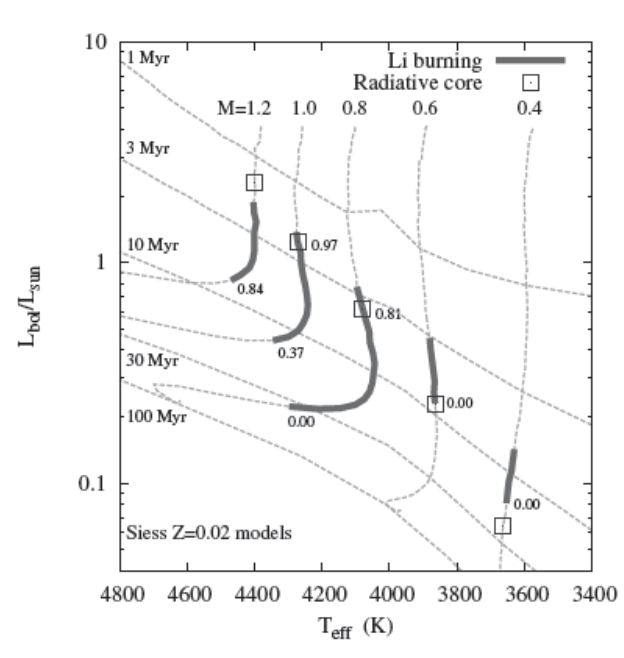
\includegraphics[width=0.5\textwidth]{img/tesis/isochrones.pdf}
	\caption {Secuencias evolutivas (en $\msun$) e isócronas (en Myr) para estrellas de baja masa comprendidas entre 0.4 y 1.2 $\msun$ y metalicidad Z=0.02. Se indican las franjas temporales en las que se produce el agotamiento fotosférico de Li y el desarrollo de un núcleo radiativo. Los números a la derecha de los intervalos de destrucción de Li indican la fracción fotosférica de éste que queda en el punto donde se desarrolla el núcleo radiativo y al final de su combustión, figura de Jeffries (2004).}
	\label{fig:isocrhones}
\end{figure}

La Figura \ref{fig:isocrhones} muestra la fase de PMS para modelos de distintas masas iniciales. Asimismo, se indican la fase de quema de Li y el momento de aparición del núcleo radiativo. Como se puede ver, las estrellas con M < 0.35 $\msun$ que se encuentran en la PMS tienen una estructura relativamente sencilla: son totalmente convectivas hasta que consiguen alcanzar la Termination Age Main Sequence (TAMS). A medida que la estrella va reduciendo su volumen según desciende a lo largo de la traza de Hayashi, su núcleo se va calentando, pero el gradiente de temperatura se mantiene muy cerca del gradiente adiabático, el cual delimita la frontera entre un núcleo radiativo o convectivo. Esta situación se mantiene para la práctica totalidad de la estrella, con la excepción de las capas superficiales. El Li comienza a arder en reacciones de captura protónica cuando la temperatura central, Tc=2.5 $10^{6} K$ y, debido a que la tasa de reacción es tan sensible a la temperatura para densidades típicas de PMS \cite{Randich2006} y a que el mezclado convectivo se produce de forma tan rápida, todo el Li se quema en una pequeña fracción de tiempo. Por otra parte, se ha contrastado que la edad a la que se produce el agotamiento de Li es inversamente proporcional a la masa de la estrella, es decir, aumenta según disminuye la masa hasta que se alcanza el límite de M < 0.06 $\msun$, ya que en este tipo de estrellas nunca llegará a alcanzarse una temperatura lo suficientemente alta como para poder quemar Li.\par

En las estrellas M > 0.35 $\msun$, el proceso de agotamiento del Li es bastante más complejo. Tienen densidades centrales más bajas y a medida que la Tc aumenta durante la contracción del PMS, la opacidad cae lo suficiente como para que el gradiente de temperatura se vuelva subadiabático, es decir, inhibe el proceso de mezclado y se forma un núcleo radiativo que empuja hacia afuera para incluir una fracción rápidamente creciente de la masa estelar.  Para M <  $\msun$ solo existe una pequeña ventana de oportunidad en la que poder quemar un poco de Li antes de que se desarrolle el núcleo radiativo (aproximadamente a 2 Myr para 1 $\msun$). Como se puede observar en la Figura \ref{fig:isocrhones}, para M < 0.6 $\msun$ el núcleo radiativo se desarrolla antes de que la quema de Li esté completa. A falta de mezcla por convección, el material agotado de Li no puede llegar a la fotosfera y una vez que la temperatura en la base de la zona de convección cae por debajo del umbral de combustión de Li, el agotamiento de Li fotosférico se detiene. Para una estrella de 1 $\msun$, el agotamiento de Li fotosférico comienza aproximadamente a los 2 Myr y debería de terminar al alcanzar los 15 Myr.\par

Los estudios sobre el Li en los cúmulos muy jóvenes indican que las estrellas de tipo solar sufren muy poco (si es que lo hay) agotamiento de Li durante las fases de la PMS  \cite{Jeffries2004}. Al mismo tiempo, se ha dedicado una gran cantidad de esfuerzo observacional al muestreo de abundancia de Li y también del Be \cite{Mena2011, DelgadoMena2014} con el objetivo de poner restricciones empíricas más severas a los mecanismos propuestos.

\section{Evolución del Li en la secuencia principal (MS)}
Como ya mencionó en el trabajo \cite{Zappala1972} hace algo más de cuatro décadas, la medición de Li en cúmulos más antiguos que los Hyades es una herramienta clave para investigar el agotamiento que sufre el Li en la MS, además de las escalas de tiempo en las que ocurre este proceso. Ahora, más de 40 años después, se han llevado nuevas mediciones de Li para varios cúmulos antiguos, incluyendo NGC 752 y M 67 \cite{Sestito2006} que han permitido caracterizar de manera más completa la dispersión de Li en estrellas de tipo solar y con metalicidad y edad similar al Sol \cite{Sestito2005}.\par

Basándonos en los resultados de los modelos de evolución estándar que solo tienen en cuenta los procesos de convección como los mecanismos a través de los cuales se produce el mezclado, solo debería agotarse el Li en la PMS, ya que es en esta fase cuando las estrellas exhiben una envolvente convectiva profunda con una base lo suficientemente caliente como para quemar el Li. Por otra parte, estos mismos modelos predicen que este proceso se detiene en la MS para estrellas de tipo solar o aquéllas más calientes. Sin embargo, los estudios llevados a cabo con cúmulos abiertos han revelado A(Li) 10 veces inferior respecto a los valores esperados en estrellas en su MS \cite{Sestito2005}, y de hecho, nuestro propio Sol presenta un agotamiento una A(Li) 100 veces inferior si comparamos con la abundancia de Li detectada en los meteoritos \cite{Lodders2003}.\par

\begin{figure}
	\centering
	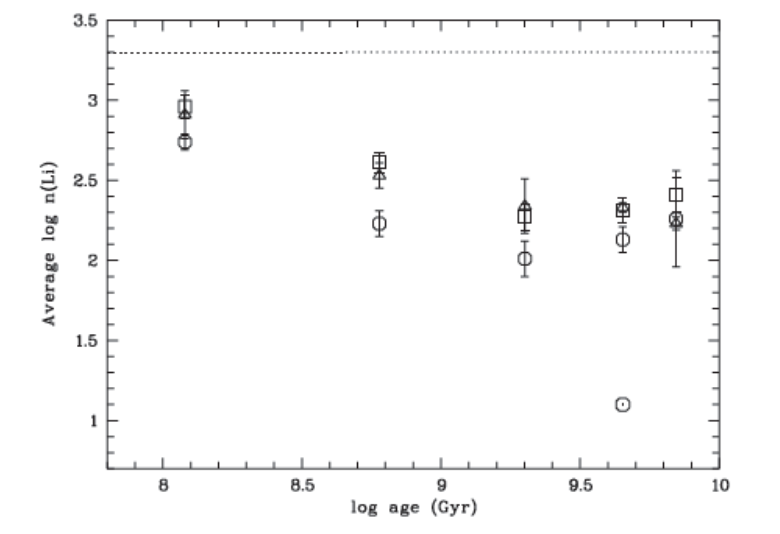
\includegraphics[width=0.5\textwidth]{img/tesis/li_abundances_vs_age.pdf}
	\caption{Abundancia media de Li en función de la edad. Las masas y edades han sido estimadas a partir de las temperaturas efectivas hacienda uso de isócronas. Las abundancias de Li se denotan mediante la notación log n(Li) = N (Li)/N (H) + 12. Los diferentes símbolos indican estrellas con diferentes masas, a saber: 1$\pm$0.02 $\msun$ (círculos), 1.05$\pm$0.02 $\msun$ (cuadrados) y 1.1 $\pm$0.02 $\msun$ (triángulos). El Sol ($\odot$) también se muestra. La línea horizontal indica la abundancia primigenia de Li, figura de \cite{Randich2006}.}
	\label{fig:li_abundances_vs_age}
\end{figure}

La Figura \ref{fig:li_abundances_vs_age} muestra que la evolución del Li desde aproximadamente 100 Myr hasta 6-8 Gyr es similar para los 3 rangos de masas. Se observa que los valores log n(Li) declinan a una ratio casi constante a medida que la estrella envejece. Esto ocurre así hasta aproximadamente los 2 Gyr, momento a partir del cual el agotamiento del Li parece virtualmente detenerse y las abundancias tienden a converger hacia los valores del Spite plateau, la línea de base en la A(Li) encontrada para estrellas antiguas (o de población II) y que por tanto se formaron a partir de material no alterado por otros procesos, que orbitan el halo galáctico. \par

\section{Mecanismos de destrucción de Li}
En este apartado procedemos a enumerar las diferentes opciones que actualmente defienden las principales líneas de investigación para intentar establecer una relación causa-efecto para la discrepancia de la abundancia de Li detectada en las fotosferas de estrellas de tipo solar.\par

\subsection{Li y metalicidad}
Durante más de tres décadas, las estrellas con baja metalicidad ([Fe/H] < -1.0 dex), también denominadas de Población II, se han caracterizado por exhibir una relación bastante estable entre la abundancia de Li y su metalicidad \cite{Guiglion2016}. Este nivel quedó inicialmente vinculado a la abundancia primordial asociada al Li, aunque esta situación ha cambiado a la luz de los resultados obtenidos por la misión Wilkinson Microwave Anisotropy Probe (WMAP), que han propiciado que la abundancia de este elemento predicha por el modelo Estándar de Nucleosíntesis para el Big Bang (SBBN) haya pasado a estimarse en 2.6 dex \cite{Spergel2003}. Este dato, sin embargo, entra en contradicción con la abundancia de Li medida en enanas viejas de baja metalicidad  (A(Li) $\simeq$ 2.2 dex) situadas en el halo de la galaxia conocido como el Spite plateau \cite{Spite1982}. Además, para estrellas de baja metalicidad (\ref{fig:li_abundances_sbbn}) se ha encontrado que la abundancia de Li no parece guardar relación con la metalicidad de la estrella \cite{Fu2015}.\par


\begin{figure}
	\centering
	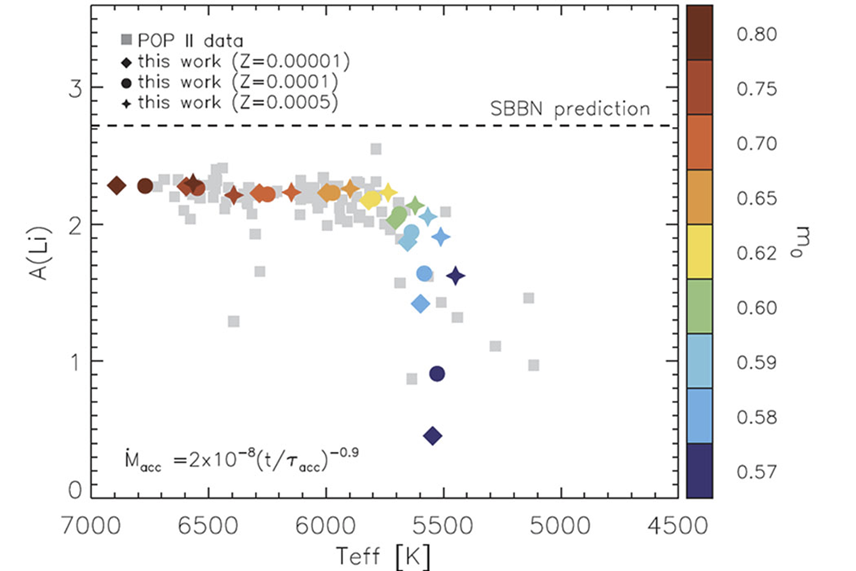
\includegraphics[width=0.5\textwidth]{img/tesis/li_abundances_sbbn.pdf}
	\caption{La abundancia de Li derivada para estrellas de baja metalicidad situadas en la secuencia principal es aproximadamente tres veces menor que el valor de Li primordial predicho por la SBBN, figura de \cite{Fu2015}.}
	\label{fig:li_abundances_sbbn}
\end{figure}

Se han realizado investigaciones para intentar vislumbrar si existe una relación entre las concentraciones de Li y la metalicidad de la nube de la que surgen las estrellas \cite{Pinsonneault1997, BarradoyNavascues2001}). Parece que esto no es así y el agotamiento del Li observado no sugiere que dependa de manera concluyente del contenido en elementos metálicos presente en esa nube primordial \cite{Guiglion2016}. Se ha contrastado que tanto para los cúmulos jóvenes (alta metalicidad) como para los antiguos (baja metalicidad), cuyos niveles de metalicidad varían aproximadamente $\pm$0.2 dex con respecto a la metalicidad de nuestro Sol, parecen compartir una distribución de Li muy similar \cite{Sestito2005}. Adicionalmente, se ha medido que la abundancia de Li medida en el Sol es mucho más baja que la que presentada por otras estrellas similares situadas en su vecindad \cite{Reddy2003}. Esta variación es más acusada que la detectada para otros tipos de elementos presentes en él.\par

Por otro lado, otros autores \cite{Sestito2005} defienden que la amplia gama de abundancias de Li observadas en estrellas similares al Sol y cercanas a éste es más fácilmente explicable si se establece una dependencia entre la abundancia de Li, la edad y masa de la estrella.\par

\subsection{Li y convección}
Una gran cantidad de trabajo teórico y observacional se ha dedicado a la comprensión de Li y su evolución, las evidencias acumuladas no concuerdan con las predicciones de los modelos estándar \cite{Sestito2005}; entendiendo por estándar a aquellos modelos que incluyen sólo los mecanismos de convección como proceso de mezcla y no tienen en cuenta fenómenos que podrían influir también como el transporte, como la difusión, las ondas de gravedad (nos referimos a ondas en el fluido de la estrella inducidas por la gravedad), la pérdida de momento angular o la presencia de planetas.\par

En las estrellas de tipo solar, la quema de Li se produce a una temperatura aproximada de 2.5 $10^{6} K$ mediante las reacciones de captura protónica que acontecen en interiores estelares. Por lo tanto, si se mantiene de manera continuada en el tiempo el mecanismo que transporta el Li entre la zona de convección exterior químicamente mixta y las regiones más profundas que poseen temperaturas lo suficientemente altas, éste acabará siendo destruido y su abundancia fotosférica disminuirá, llegando en algunos casos prácticamente a desparecer de la superficie estelar \cite{DelgadoMena2014}.\par

A su vez, la abundancia de Li medida en la fotosfera nos sirve también para realizar la calibración de modelos de evolución estelar. Sin embargo, es preciso mencionar que para que este planteamiento sea coherente, hay que suponer que la abundancia inicial de Li es conocida y que éste es única y exclusivamente destruido mediante reacciones nucleares.\par

\subsection{Li y difusión}
Un factor determinante para conocer la fase evolutiva en la que se encuentra una estrella es su composición química interna. Los modelos estándar consideran, como hemos apuntado anteriormente, a los procesos desencadenados por reacciones nucleares y por convección como los únicos que pueden modificar este perfil químico. Sin embargo, la difusión química de elementos también puede alterar este perfil y puede considerarse como otro mecanismo que contribuye a la disminución de la abundancia de litio en la superficie que tiene lugar a lo largo de MS. Este sería otro factor a tener en cuenta que contribuiría a poder explicar por qué la abundancia solar fotosférica es mucho menor que la meteórica. Sin embargo, este proceso estelar a largo plazo no puede ser observado directamente en las estrellas.\par

En el trabajo de \cite{Richard2004}, mostraron que la menor abundancia de Li observada en las estrellas de tipo Población II es el resultado del agotamiento de Li producido por el efecto de difusión atómica que entra en competencia con los procesos de mezclado en las zonas radiativas de estas estrellas.\par

La difusión microscópica acorta la vida útil de la secuencia principal y conduce a un agotamiento de los elementos superficiales. El modelo solar requiere la inclusión de difusión microscópica, de lo contrario ni siquiera la edad del Sol se podría producir correctamente \cite{Thoul1993}.\par

\subsection{Li y exoplanetas}
El descubrimiento de un gran número de exoplanetas durante las dos últimas décadas \cite{Mayor1995, Bonfils2018} ha significado un importante empuje para la comunidad científica en el campo de la astrofísica. Aparte de las consecuencias directas derivadas de poder estudiar los nuevos planetas descubiertos más allá de nuestro sistema solar, lo que ya es de por sí extremadamente interesante, no lo es menos la observación de sus estrellas anfitrionas, ya que éstas pueden llegar a aportar información muy valiosa acerca de las características globales, composición y formación de los sistemas planetarios extrasolares que albergan.\par

La hipótesis de que la variabilidad de concentración de Li en las estrellas puede ser debida a una posible correlación entre la presencia de planetas es una línea de trabajo de diversos estudios \cite{Israelian2009, DelgadoMena2014, Figueira2014}. Estas investigaciones apuntan a que esta presencia podría ser el desencadenante de la discrepancia en la abundancia de Li medidas en estrellas de tipo solar. Para nuestro Sol, ésta es unas 140 veces inferior a la que le correspondería a su modelo estelar \cite{Israelian2009}, aunque la temperatura en la BCZ no es lo suficientemente alta como para quemarlo.\par

En un primer momento, esta línea de investigación no se encontraba suficientemente fundamentada en evidencias que apoyasen este planteamiento, y esto se debía a la escasa disponibilidad de datos sobre estrellas que tuviesen sistemas planetarios asociados. En los últimos años, gracias a satélites como CoRoT \cite{Baglin2006} y Kepler \cite{Borucki2010}, dedicados a la búsqueda de planetas extrasolares, se han podido obtener datos de un gran número de estrellas con sistemas planetarios asociados. Esta nueva situación ha derivado en la realización de nuevos trabajos, o en la revisión de otros anteriores, en los que se han podido realizar nuevos estudios comparativos más amplios y sin sesgo en lo que se refiere a poder comparar estrellas con y sin sistemas planetarios. Estos nuevos trabajos han arrojado evidencias, tanto a favor como en contra, sobre la existencia de una relación directa entre la menor abundancia de Li en las estrellas con planetas con respecto a las que no tienen. Entre los primeros, tenemos el trabajo de \cite{Israelian2009}, en el que sus autores afirman que tras el análisis comparativo de un total de 133 estrellas en el rango de temperaturas que va de los $5600..5900 K$, de las que 30 de ellas albergan planetas y 103 no, encontraron que la gran mayoría de aquéllas que poseían planetas presentaron una disminución acusada en la abundancia de Li respecto de las que no tenían planetas (\ref{fig:li_abundances_planets}). También indican que por encima y por debajo de ese rango de temperaturas no parece existir relación alguna con la presencia o no de planetas, extremo que justifican al alegar que para estrellas con una temperatura superficial por encima de los $5850 K$, las capas convectivas de las estrellas más masivas que el Sol no son lo suficientemente profundas y además se encuentran demasiado alejadas como para alcanzar las regiones interiores de las estrella donde se alcanza una temperatura suficiente para quemar el Li.\par

Incluso su trabajo va más allá al afirmar que la menor abundancia de Li en estrellas con una temperatura efectiva restringida al rango $\tsun \pm 80$ K ($\tsun = 5777$ K) es una constante en las estrellas con planetas que se encuentran en su MS y que este resultado es independiente de la temperatura efectiva o la masa de las mismas. Por otro lado, el Li apenas se ve afectado en las estrellas menos evolucionadas, más calientes ($\teff > 6000$ K) y masivas, ya que éstas presentan una capa convectiva delgada. Por tanto, en este tipo de estrellas no existe una relación directa entre la temperatura de las mismas y la concentración de Li.\par

\begin{figure}
	\centering
	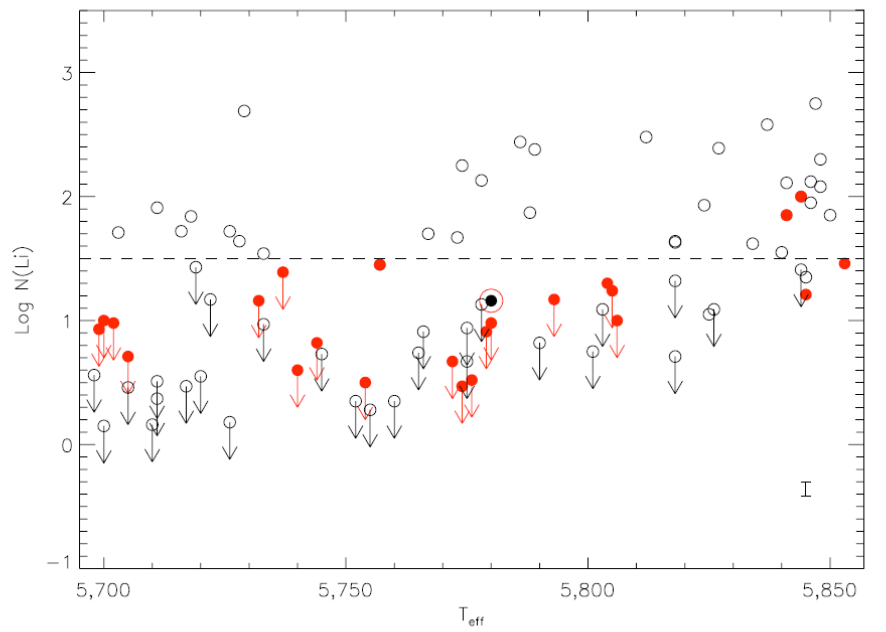
\includegraphics[width=0.5\textwidth]{img/tesis/li_abundances_planets.pdf}
	\caption{Abundancia de Li vs temperatura efectiva en estrellas de tipo solar con y sin planetas. Las estrellas con planetas vienen representadas por los círculos rojos y las sin planetas por los círculos vacíos. El Sol queda representado por el punto negro rodeado de un círculo rojo, figura de \cite{Israelian2009}.}
	\label{fig:li_abundances_planets}
\end{figure}

Recientemente, se ha postulado otra alternativa por la que la presencia de planetas alrededor de una estrella podría afectar la evolución de la abundancia de Li fotosférico \cite{Bouvier2008}. El autor mantiene que, en el contexto de las estrellas de tipo solar en las que se han detectado exoplanetas respecto de las que no los albergan, la menor concentración de Li en las primeras puede ser el resultado de su historia rotacional. Afirma que, mediante el desarrollo de modelos de evolución de tipo solar incluyendo rotación, tanto para rotadores lentos (unas 5 veces mayor la velocidad de rotación del Sol) como rápidos (unas 70 veces mayor), que hacen evolucionar desde la PMS hasta la edad actual de nuestro Sol, han conseguido encontrar pruebas de que las estrellas con una rotación menor desarrollan un alto grado de rotación diferencial entre el núcleo radiativo y la envolvente convectiva, mientras que los rotadores rápidos evolucionan con poco desacoplamiento entre núcleo y envoltura. A raíz de esta fuerte rotación diferencial en la base de la envoltura convectiva, en los rotadores lentos el proceso de destrucción del Li se vuelve más eficiente, concluyendo que las estrellas que albergan exoplanetas y presentan un agotamiento del Li debieron de ser rotadores lentos durante ZAMS y que esto se debió a una interacción duradera entre la estrella y el disco plotoplanetario durante la PMS. De este planteamiento también se desprende que la vida de los discos debe ser más longeva (>5 Myr) de lo esperado y, posiblemente, también sea una condición necesaria para que se produzca la formación de planetas masivos y su posterior migración hacia zonas más exteriores del sistema planetario.\par

Asimismo, no faltan tampoco los referentes bibliográficos que defienden que no existe relación directa alguna entre la menor abundancia de Li detectada en la atmósfera de las estrellas que albergan planetas y las que no los tienen. En el trabajo de \cite{Baumann2010} se procede a analizar 117 estrellas con propiedades semejantes a nuestro Sol. Sus autores sostienen que las evidencias encontradas por otros investigadores en la dirección de la existencia de una relación entre las abundancias de Li detectadas y las estrellas que albergan planetas, se deben única y exclusivamente a consideraciones sesgadas y errores sistemáticos producidos durante el análisis de los datos recopilados. Por el contrario, estos mismos autores sostienen que sí existen evidencias claras entre la abundancia de Li de una estrella con su edad y la metalicidad de la misma. Por otra parte, la ingestión de un planeta “fallido” podría ser la causa por la que se produce un aumento de la abundancia de este elemento en la superficie de las estrellas.\par

\subsection{Li y rotación}
El impacto de la rotación tanto en la PMS como en el agotamiento del Li para las estrellas de tipo solar ha sido ampliamente debatido en el pasado \cite{Pinsonneault1997,Jeffries2004,Somers2014} y revisado más recientemente sobre la base de la disponibilidad de medidas más precisas \cite{Bouvier2016}. Los resultados sugieren una conexión entre la velocidad de rotación de las estrellas y la A(Li) detectada en sus atmósferas estelares, de modo que las estrellas que giran más rápido destruyen menos Li que las que lo hacen de manera más lenta. De alguna manera los resultados publicados por \cite{Bouvier2016} son inesperados ya que apuntan en una dirección diametralmente opuesta a los de trabajos anteriores, en los que se predecía que las estrellas que rotan más rápidamente deberían de destruir una mayor cantidad de Li.\par 

Para explicar esta tendencia, es necesario recurrir a mecanismos adicionales que vinculen el agotamiento del Li y la rotación. Esta aparente contradicción de los resultados de diferentes trabajos no tiene por qué se tal. De hecho se plantean diferentes ideas que pueden ayudar a entender las discrepancias, entre las que se encuentra el acoplamiento de las estrellas con sus disco proto-estelar, que influiría en los mecanismos de mezclado ocasionados por la rotación \cite{Bouvier2008, Eggenberger2012}, la influencia de campos magnéticos \cite{Eggenberger2009} que tienen la propiedad de transmitir el momento angular (AM) de forma mucho más eficaz que inducir la mezcla \cite{Denissenkov2007}. Como consecuencia de este incremento en la eficiencia del transporte del AM, se reduce la cantidad de rotación diferencial entre las zonas radiativa y convectiva de la estrella (se fomenta una rotación de cuerpo sólido), así como las inestabilidades rotacionales inducidas. La acreción de material \cite{Baraffe2010} también se postula como una posibilidad para explicar la menor A(Li) para estrellas en el mismo rango de masas y edad. Episodios periódicos de acreción de material por parte de la estrella conducen a desarrollar temperaturas centrales significativamente más altas. A consecuencia de ello, una mayor cantidad de Li puede ser destruido.\par


\subsection{A qué se debe esta merma de Li}
Como hemos enumerado en los puntos anteriores, existe una propuesta amplia de potenciales mecanismos que podrían, por una parte, gobernar el ciclo de vida del Li, y por otra, ayudar a entender a qué se deben las discrepancias entre las observaciones y los resultados arrojados por los modelos. Sirva como ejemplo la línea de trabajo de \cite{Ramirez2012} en el que sus autores miden las abundancias de Li de una gran muestra de estrellas para encontrar correlaciones entre éstas y otras propiedades. Tales correlaciones deberían poder ayudar a determinar exactamente cómo se destruye el Li en las estrellas y cómo la abundancia galáctica de este elemento ha cambiado durante la vida de la Vía Láctea.\par 

De manera genérica, estos mecanismos pueden agruparse en dos ideas principales. Por un lado, los que abogan por la propuesta de que la abundancia de este elemento en la superficie de las estrellas podría ser menor de la que los modelos predicen debido a que el Li podría haberse transformado en elementos más pesados mediante reacciones nucleares. El mayor inconveniente de este planteamiento es que la temperatura requerida para fusionar el Li y crear otros elementos es normalmente más elevada que la que puede ser alcanzada por las capas externas convectivas presentes en estrellas similares a nuestro Sol. Por esa razón, se ha propuesto una segunda explicación alternativa que plantea que el Li podría haberse mezclado en las capas más profundas de la estrella y de este modo, haber desaparecido de las zonas exteriores \cite{Pinsonneault1997}.\par



\section{El litio y las reacciones nucleares} \label{sec:li_reac_nuc}
Hasta aquí hemos presentado los posibles mecanismos que influyen de manera más o menos directa en la destrucción del Li, pero finalmente éste se destruye porque se produce una "quema" del mismo cuando las condiciones en el interior estelar son las adecuadas para que se produzcan una serie de reacciones nucleares. Como consecuencia, para poder obtener las abundancias de Li aL final de la TAMS, primeramente necesitamos conocer qué reacciones nucleares son las responsables de su creación. De acuerdo a Cox y Giuli \cite{Cox1968}, en las condiciones de temperatura y densidad que se dan en el interior de una estrella de tipo solar (1.0 $\msun$), el tiempo de vida de los elementos más ligeros: $\isotope[2]{H}$, $\isotope[3]{H}$, $\isotope[6]{Li}$, $\isotope[9]{B}$, $\isotope[10]{B}$ y $\isotope[11]{B}$ y los resultantes de combinarse con el H a través de las reacciones de cadena protón-protón en sus variantes I, II y III, tienen un tiempo de vida que va desde los pocos segundos hasta los aproximadamente $10^4$ años. Por lo tanto, todos estos elementos deberían de consumirse en las etapas iniciales de vida de la estrella, tan pronto su interior ronde los $10^7$ K.\par

La cadena de reacción protón-protón I es la cadena de reacciones dominantes en estrellas de tamaño solar o menor. El primer paso conduce a la fusión de dos núcleos de hidrógeno $\isotope[1]{H}$ (protones) a deuterio $\isotope[2]{H}$, liberando un positrón y un neutrino al transformar un protón en un neutrón. El positrón resultante de dicha reacción se aniquila inmediatamente con un electrón y su masa se convierte en energía liberada a través de dos fotones gamma. Tras esta reacción, el deuterio producido en el primer paso se puede fusionar con otro hidrógeno para producir un isótopo ligero de helio $\isotope[3]{He}$. A partir de este punto la reacción se subdivide en tres ramas diferentes que desembocan todas en la generación de un núcleo $\isotope[4]{He}$. En la variante I (Figura \ref{fig:pp-I}), éste se produce por la fusión de dos núcleos de $\isotope[3]{He}$.\par


\begin{figure}
	\centering
	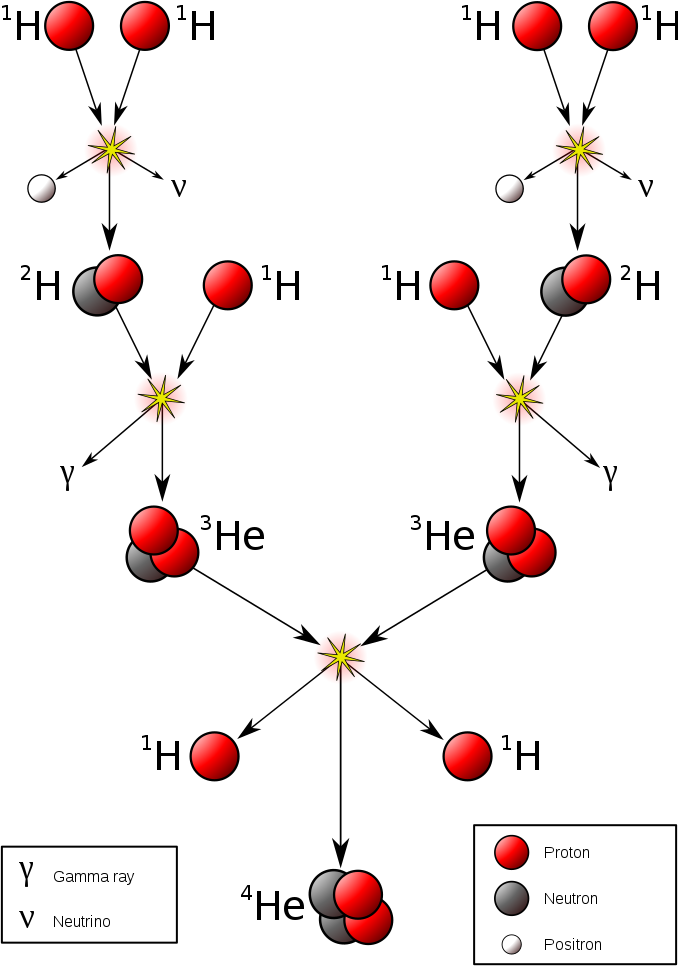
\includegraphics[width=0.4\textwidth]{img/tesis/pp-I.png}
	\caption {Cadena de reacciones protón-protón I (pp-I)}
	\label{fig:pp-I}
\end{figure}

En las otras dos variantes, II (\ref{fig:pp-II}) y III (\ref{fig:pp-III}), se requiere del $\isotope[4]{He}$ previamente producido y ambas cadenas surgen a consecuencia de los dos caminos que el $\isotope[7]{Be}$ puede tomar. Como podemos observar un primer paso en común para las tres cadenas es la fusión de dos protones en deuterio.

\begin{figure}
	\centering
	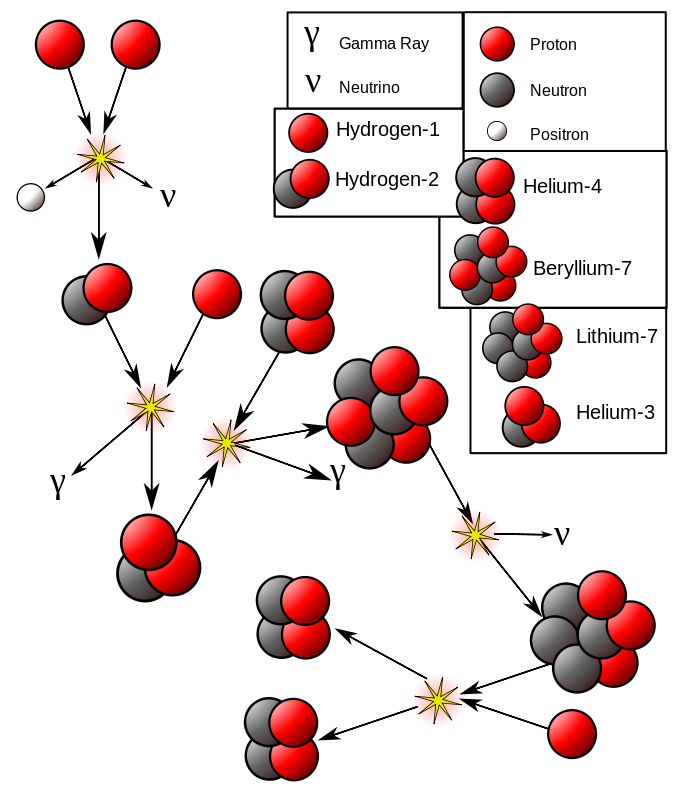
\includegraphics[width=0.4\textwidth]{img/tesis/pp-II.png}
	\caption {Cadena de reacciones protón-protón II (pp-II)}
	\label{fig:pp-II}
\end{figure}

De particular interés para este trabajo es la variante II, ya que en ella es donde se produce $\isotope[7]{Li}$. En esta variante de la reacción se requieren temperaturas del orden de $1.4x10^7..2.3x10^7$ K. Bajo estas condiciones los isótopos estables de $\isotope[3]{He}$ se fusionan con núcleos de $\isotope[4]{He}$ para dar lugar a $\isotope[7]{Be}$, que tras capturar un electrón forma $\isotope[7]{Li}$. Finalmente, $\isotope[7]{Li}$ se fusiona con un protón para dar lugar a dos núcleos de $\isotope[4]{He}$.\par

\begin{figure}
	\centering
	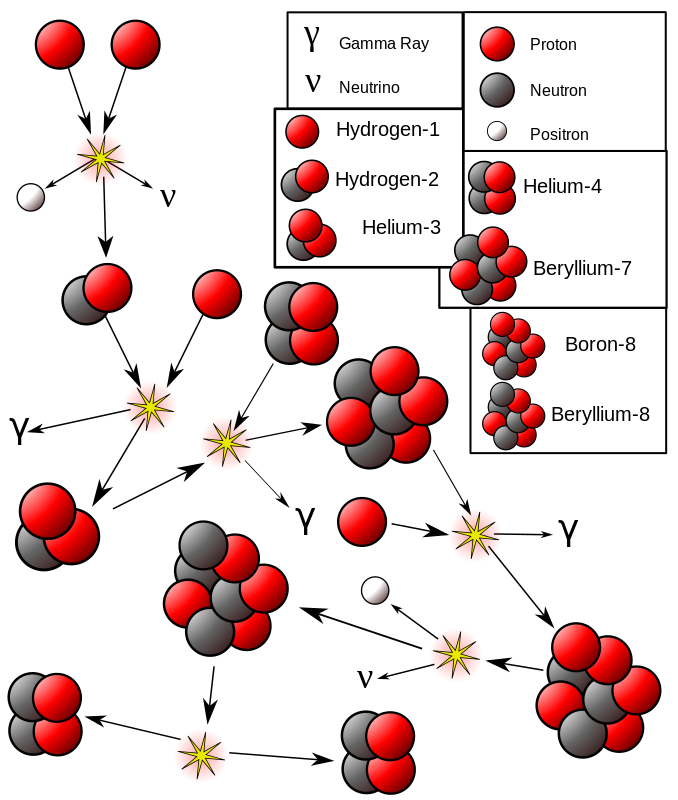
\includegraphics[width=0.4\textwidth]{img/tesis/pp-III.png}
	\caption {Cadena de reacciones protón-protón III (pp-III)}
	\label{fig:pp-III}
\end{figure}

La variante III es la rama dominante cuando se alcanzan temperaturas superiores a los $2.3x10^7$ K. En esta rama, el $\isotope[7]{Li}$ se fusiona con un protón para formar un núcleo de $\isotope[7]{Li}$, que se descompone en un núcleo de $\isotope[8]{Be}$ y un positrón. Luego, el $\isotope[8]{Be}$ se descompone en dos núcleos de $\isotope[4]{He}$.\par

Los tres tipos de variantes ocurren de manera simultánea en el interior de las estrellas, pero unas son más frecuentes que otras. De acuerdo a las investigaciones teóricas, parcialmente soportadas por las medidas de neutrinos procedentes del Sol, se calcula que el 86\% de las reacciones se corresponden con las de tipo I, un 14\% con la de tipo II, y solo un 0.02\% con las de tipo III \cite{Scholz2018}.


De manera similar, la vida media de los isótopos involucrados en el ciclo CNO (Figura \ref{fig:ciclo-cno}) al recombinarse con el H dominante en esas primeras etapas debería de rondar los $10^6$-$10^7$ años. Sin embargo, este ciclo de fusión a través del cual las estrellas también generan He a partir del H es más representativo de estrellas con una masa superior a 1.3 $\msun$. 


\begin{figure}
	\centering
	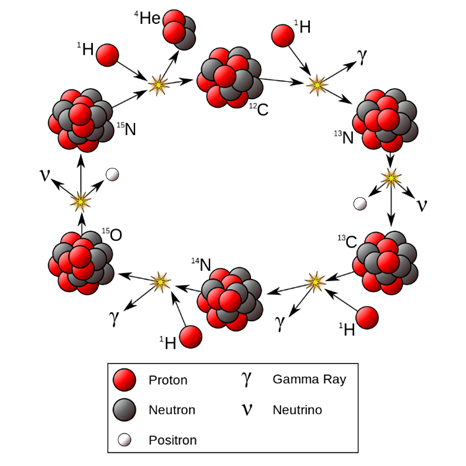
\includegraphics[width=0.5\textwidth]{img/tesis/ciclo CNO.png}
	\caption {Cadena de reacciones del ciclo CNO}
	\label{fig:ciclo-cno}
\end{figure}


\endinput
%--------------------------------------------------------------------
% FIN DEL CAPÍTULO. 
%--------------------------------------------------------------------


\cleardoublepage
\part{Ciencia de datos}
% !TeX root = ../libro.tex
% !TeX encoding = utf8

\chapter{Ciencia de datos}\label{ch:octavo-capitulo}
\section{Introducción}
La ciencia de datos es un campo interdisciplinario que utiliza algoritmos, procedimientos y procesos para examinar grandes cantidades de datos con el fin de descubrir patrones ocultos, generar conocimientos y dirigir la toma de decisiones. Utiliza técnicas y teorías extraídas de muchos campos dentro del contexto de las matemáticas, estadísticas, programación, análisis y aprendizaje automático para descubrir conocimientos accionables a partir de conjuntos de datos.\par

En el contexto de la astrofísica, la ciencia de datos juega un papel crucial. Los astrofísicos y físicos de partículas utilizan instrumentación de última generación en telescopios y aceleradores para estudiar el Universo tanto en las escalas más grandes como en las más pequeñas. Los enormes conjuntos de datos a escala de petabytes que resultan de las diferentes observaciones y experimentos se explotan en busca de indicios, pistas que pueden arrojar luz sobre la naturaleza de la materia oscura, la energía oscura, la evolución de los agujeros negros y la física más allá del "modelo estándar" de la cosmología y la física de partículas.\par

El desafío es reformular el modelado de datos que los astrofísicos necesitan hacer de tal manera que se puedan aplicar arquitecturas de aprendizaje automático de última generación, sin comprometer el alto nivel de control de errores sistemáticos, ni la comprensión detallada de la incertidumbre estadística, que las preguntas de física que se están abordando con extrema precisión en el siglo XXI exigen. Por lo tanto, las simulaciones nos permiten probar qué teorías son consistentes con el Universo que podemos observar. Esta es una clara demostración del poder y la necesidad de la ciencia de datos para avanzar en nuestra comprensión del universo.\par


\section{Proceso de la ciencia de datos}
El proceso de ciencia de datos es un enfoque sistemático que implica varios pasos para extraer valiosos conocimientos de los datos. Comienza con la definición del problema, que implica entender los objetivos que se persiguen y formular preguntas que pueden ser respondidas con datos. Los siguientes pasos implican la recopilación y limpieza de los datos, seguidos por el análisis exploratorio de los mismos para entender los patrones y tendencias subyacentes. Esto es continuado por la construcción y evaluación del modelo para predecir resultados o descubrir estructuras dentro de los datos. Finalmente, el modelo se despliega, se contrastan los resultados con las observaciones, y los hallazgos se comunican a las partes interesadas.\par

Desde una perspectiva científica, el proceso de ciencia de datos es crucial ya que proporciona una metodología estructurada para manejar y analizar grandes volúmenes de datos. Permite a los científicos probar hipótesis, descubrir patrones, hacer predicciones e impulsar la toma de decisiones. Cada paso en el proceso sirve a un propósito específico y contribuye al objetivo general de extraer información significativa de los datos. Por ejemplo, la limpieza de datos asegura la calidad de los datos, el análisis exploratorio de datos ayuda a entender los datos, y la construcción del modelo permite hacer predicciones e inferencias.\par

Además, la naturaleza iterativa del proceso de ciencia de datos se alinea con el método científico de investigación, que implica formar hipótesis, realizar experimentos y refinar teorías basadas en los resultados. Este proceso iterativo nos permite un aprendizaje y mejora continua. Además, el énfasis en la comunicación en el proceso de ciencia de datos asegura que los hallazgos puedan ser compartidos e implementados de manera efectiva, contribuyendo al avance del conocimiento en varios campos. Por lo tanto, el proceso de ciencia de datos no sólo es un aspecto fundamental de la toma de decisiones basada en datos, sino también un contribuyente significativo al progreso científico.\par

Dentro del proceso de datos podemos enumerar una serie de etapas encaminadas a establecer una sistemática a la hora de su ejecución. El proceso no debe contemplarse como un marco rígido que no admite alteraciones al mismos, sino como que debe ser utilizado como una herramienta que debe ser adaptada a nuestras necesidades. Dependiendo de los objetivos establecidos, de la calidad de los datos que están a nuestra disposición, algunas de las siguientes etapas se harán más necesarias que otras, más intensas en lo que a la asignación de recursos se refiere. Entre los diferentes podemos enumerar los siguientes:
 
\begin{enumerate}
	\item \textit{Definición del problema} - Este es el primer paso donde definimos el problema que estás tratando de resolver. Implica entender los objetivos de la investigación, para a continuación formular preguntas que pueden ser respondidas con datos e identificar las fuentes de datos necesarias.
	\item \textit{Recopilación de datos} - En este paso, recopilamos los datos necesarios para nuestro análisis. Esto podría implicar la consulta de sitios web, el acceso a bases de datos, generación de simulaciones.
	\item \textit{Limpieza de datos} - Una vez que tenemos los datos recopilados, es hora de limpiarlos. Esto implica manejar valores faltantes, eliminar duplicados, corregir errores y lidiar con valores atípicos.
	\item \textit{Análisis exploratorio de datos} - Este es un paso crucial donde exploramos y visualizamos los datos para entender los patrones subyacentes, las tendencias y los valores atípicos. Es una paso fundamental porque nos ayuda a generar conocimiento y formar hipótesis para un análisis más profundo.
	\item \textit{Ingeniería de características} - Esto implica crear nuevas características a partir de las existentes para representar mejor los patrones subyacentes en los datos. Es un paso esencial para mejorar el rendimiento de los modelos de aprendizaje automático. 
	\item \textit{Construcción del modelo} - Aquí, elegimos un modelo apropiado, lo entrenamos con los datos que previamente hemos obtenido para luego evaluar su rendimiento. Normalmente esto implica dividir los datos en conjuntos de entrenamiento y prueba, seleccionar un algoritmo correcto y fijar sus parámetros.
	\item \textit{Evaluación del modelo} - En este paso, evaluamos el rendimiento del utilizando métricas apropiadas. Es importante usar una métrica que se alinee con los objetivos que hemos prefijados en el paso inicial.
	\item \textit{Despliegue del modelo} - Una vez que estamos satisfecho con el rendimiento del modelo, es hora de desplegarlo. Esto podría implicar integrar el modelo en un sistema de producción, establecer un sistema de monitoreo y desarrollar un plan para el mantenimiento del mismo.
	\item \textit{Comunicación} - Finalmente, comunicamos nuestros hallazgos a las partes interesadas. Esto podría implicar la creación de artículos científicos, informes, o presentaciones que expliquen claramente tu metodología, hallazgos e implicaciones de negocio de nuestro trabajo.
\end{enumerate}

Como hemos adelantado, los pasos anteriores no de dejan de ser un marco de trabajo genérico que debe de ser adaptado a nuestras necesidades específicas. En nuestro caso en particular, no hemos recurrido al uso de herramientas de aprendizaje automático, por lo que la correspondiente etapa no ha formado parte de nuestro proceso de ciencia de datos. Del mismo modo, nuestro modelo no ha sido incorporado, integrado con ningún sistema. De momento este no ha sido el caso pero no sería descabellado pensar que pudiese pasar a incorporarse como una extensión a la herramienta que hemos utilizado para nuestras simulaciones, si lo autores de la misma lo considerasen oportuno.


\section{Catálogos de datos}
En la vastedad del cosmos, los catálogos de datos se alzan como pilares fundamentales para los investigadores en astrofísica. Estos catálogos, que contienen descripciones detalladas y metadatos, permiten comprender y acceder a la riqueza de información cósmica. Proporcionan contexto esencial para comprender los datos recopilados por telescopios y observatorios, permitiendo a los científicos explorar las coordenadas celestiales, las magnitudes estelares y las características espectrales.\par

Sus propiedades fundamentales son múltiples: en primer lugar, los catálogos permiten una búsqueda eficiente. En un campo donde la cantidad de datos es abrumadora, esta eficiencia es vital. Además, fomentan la colaboración científica al proporcionar un acceso centralizado. Los metadatos, que describen y resumen la entradas de los catálogos, son la clave para evaluar la calidad y actualidad de los datos.\par

Los catálogos proporcionan una base de referencia para comparar las propiedades simuladas con las observaciones reales. Además, nos permiten calibrar los parámetros de los modelos y refinarlos mediante la comparación detallada entre las características de las estrellas simuladas y las observadas.\par


\subsection{Gaia}
El catálogo Gaia \citep{Mignard2005} es un mapa tridimensional completo de la Vía Láctea, creado utilizando datos del telescopio espacial Gaia. Éste contiene datos de alrededor de 1.46 millardos de estrellas, entre los que se encuentra sus posiciones en el cielo, paralaje y movimiento propio. Además, incluye sus magnitudes en diferentes bandas espectrales para una gran cantidad de ellas. El catálogo Gaia es particularmente útil para estudiar estrellas similares al Sol, ya que proporciona un censo único de estrellas dentro de 100 pc de nuestro Sol. Esto lo convierte en un recurso invaluable para los astrónomos y astrofísicos que buscan comprender mejor las propiedades y la evolución de estas estrellas.\par

\subsection{Gaia-ESO Spectroscopic Survey - (GES)}
El estudio Gaia-ESO (Gaia-ESO Survey, GES) \citep{Gilmore2012,Randich2013,Randich2022} es un catálogo público enfocado al análisis espectroscópico de un número importante de estrellas recogidas en el catálogo Gaia. Se llevó a cabo con el instrumento espectrógrafo multielemento de fibra de gran conjunto (Fibre Large Array Multi Element Spectrograph, FLAMES) y el espectrógrafo Echelle ultravioleta y visual (Ultraviolet and Visual Echelle Spectrograph, UVES) en el VLT. Su objetivo es proporcionar una visión homogénea de las distribuciones de cinemática y abundancias elementales en la Vía Láctea, en el campo y en cúmulos abiertos (Open Cluster, OC), hasta magnitud 19.\par 

Dentro de la iniciativa GES se han observado más de 110 000 estrellas, proporcionando velocidades radiales y rotacionales proyectadas, parámetros estelares tales como: temperatura efectiva, gravedad superficial y metalicidad, abundancias de varios elementos, entre los que se encuentra el litio, para aproximadamente 1/3 de la muestra, y parámetros específicos para rastrear la acreción y actividad en estrellas jóvenes. El catálogo GES es único en lo que se refiere a la observación de estrellas de todos los tipos espectrales con análisis dedicados y especializados, lo que la hace particularmente útil para estudiar estrellas similares al Sol.\par


\section{Herramientas}
\subsection{Modules for Experiments in Stellar Astrophysics - MESA}
Para la realización de este tesis doctoral nos hemos apoyado en la herramienta de evolución estelar MESA (Modules for Experiments in Stellar Astrophysics). MESA ha jugado un papel fundamental en nuestra investigación y por ello, debido a su importancia, le hemos dedicado un capítulo en exclusiva en el que entramos a fondo en sus características, estructura, módulos que lo componen, y muy especialmente en cómo extender la física que incorpora sus modelos mediante la programación de nuestras propias rutinas.\par


\subsection{Octave} \label{sec:tool_octave}
GNU Octave es un lenguaje de programación de alto nivel destinado principalmente a cálculos numéricos. Es un conjunto de software libre y de código abierto que proporciona una interfaz de línea de comandos conveniente para resolver problemas lineales y no lineales numéricamente. La sintaxis de Octave es en gran medida compatible con MATLAB, lo que lo convierte en una alternativa popular para los usuarios que necesitan una solución rentable.\par 

Esta herramienta también proporciona amplias capacidades gráficas para la visualización y manipulación de datos. Octave puede ser extendido por paquetes, permitiendo a los usuarios añadir más funcionalidades según sea necesario. Puede ser ejecutado en modo visual, como una consola, o invocado como parte de un script de entorno. Octave está disponible para varios sistemas operativos, incluyendo GNU/Linux, macOS, BSD y Microsoft Windows.

\subsection{Tool for OPerations on Catalogues And Tables - TOPCAT} \label{sec:tool_topcat}
TOPCAT, acrónimo de \textit{Tool for OPerations on Catalogues And Tables}, es un visor y editor gráfico altamente versátil e interactivo para datos tabulares. Está diseñado para trabajar con datos astronómicos, pero puede ser utilizado para cualquier tipo de datos en formato tabular. Proporciona un entorno dinámico donde los datos pueden ser cargados, visualizados, editados y analizados. TOPCAT soporta varios formatos de datos y puede gestionar tanto archivos locales como remotos, lo que lo convierte en una herramienta flexible para la manipulación de datos.\par

En cuanto a la extracción de datos, TOPCAT permite a los usuarios ver y editar datos de celdas a través de un navegador, y tiene visores para imágenes y espectros. También se incluye un visor de trazado del cielo para datos astronómicos. Además, proporciona funciones estadísticas para analizar los datos, y capacidades de coincidencia cruzada para comparar diferentes catálogos. La herramienta también soporta scripting para tareas automatizadas. Estas características hacen de TOPCAT una herramienta integral para la extracción y análisis de datos en el campo de la astronomía y más allá.\par

TOPCAT es particularmente útil para el observatorio virtual (Virtual Observatory, VO). Ésta es una aplicación de escritorio para el análisis interactivo de datos en formato tabular, especialmente catálogos de fuentes. TOPCAT puede acceder a servicios de datos externos. También puede comunicarse con otras herramientas astronómicas a través del protocolo simple de mensajería de aplicaciones (Simple Application Messaging Protocol, SAMP). Esto permite una integración perfecta de TOPCAT en el entorno del VO, permitiendo a los usuarios recuperar y analizar datos de varios servicios.\par

Cuando se trata de extraer datos de diferentes catálogos astronómicos, TOPCAT proporciona una gama de funcionalidades, como las de leer y escribir tablas en varios formatos como FITS, VOTable, CSV. Esto hace posible trabajar con una amplia variedad de catálogos astronómicos. Por ejemplo, se puede usar TOPCAT para acceder a un catálogo de estrellas contenidas en la base de datos Gaia. Además, TOPCAT ofrece características para el cruce de correspondencias, que es crucial al comparar diferentes catálogos. En el Listado \ref{lst:consulta} podemos observar la consulta que hemos utilizado para seleccionar del catálogo GES las estrellas pertenecientes a OC's con un nivel de confianza >= 95\%. Para cada una de ellas obtenemos su temperatura efectiva, la gravedad superficial, su metalicidad, la abundancia de Li, y los valores de error asociados a cada uno de esos parámetros.\par


\begin{lstlisting}[language=SQL, float, caption={Consulta TOPCAT sobre el catálogo GES DR5 para obtener los componentes de los cúmulos abiertos para los cuales se ha determinado una pertenecia mínima del 0.95\%. Las columnas obtenidas informan sobre la identificador de la estrella, $\teff$, $\gsurf$, $\feh$, A(Li) y sus errores asociados, y el identificador del cúmulo al que pertenece.}, label={lst:consulta}]
	SELECT object,teff,e_teff,logg,e_logg,feh,e_feh,li1,e_li1,ges_fld
	FROM ges_dr5 
	WHERE ges_fld IN (
	SELECT DISTINCT ges_fld
	FROM ges_dr5 
	WHERE ges_type 
	LIKE 'GE_CL%' 
	OR ges_type LIKE 'GE_SD_OC%' 
	OR ges_type LIKE 'AR_CL%' 
	OR ges_type LIKE 'AR_SD_OC' )
	AND mem3d >= 0.95
	AND li1 IS NOT NULL
	AND feh IS NOT NULL
	AND ges_fld IS NOT NULL
	AND teff IS NOT NULL
	AND logg IS NOT NULL
	AND nn_teff IS NOT NULL
	AND nn_logg IS NOT NULL
	AND nn_feh IS NOT NULL
	ORDER BY ges_fld
\end{lstlisting}

Antes de poder realizar la consulta hay que localizar el catálogo sobre el que ejecutar la búsqueda. Como acabamos de comentar, TOPCAT es una herramienta polivalente y que sobresale a la hora de acceder a diferentes fuentes datos. Mediante el protocolo de acceso a tablas (Table Access Protocol, TAP) TOPCAT ofrece la posibilidad de realizar búsquedas entre los catálogos que soportan TAP mediante el uso de palabras claves o propiedades de los catálogos. En la Figura \ref{fig:tap_ges_service} vemos el resultado ofrecido tras realizar una búsqueda en los catálogos disponibles que están relacionados con GES.\par

\begin{figure}
	\centering
	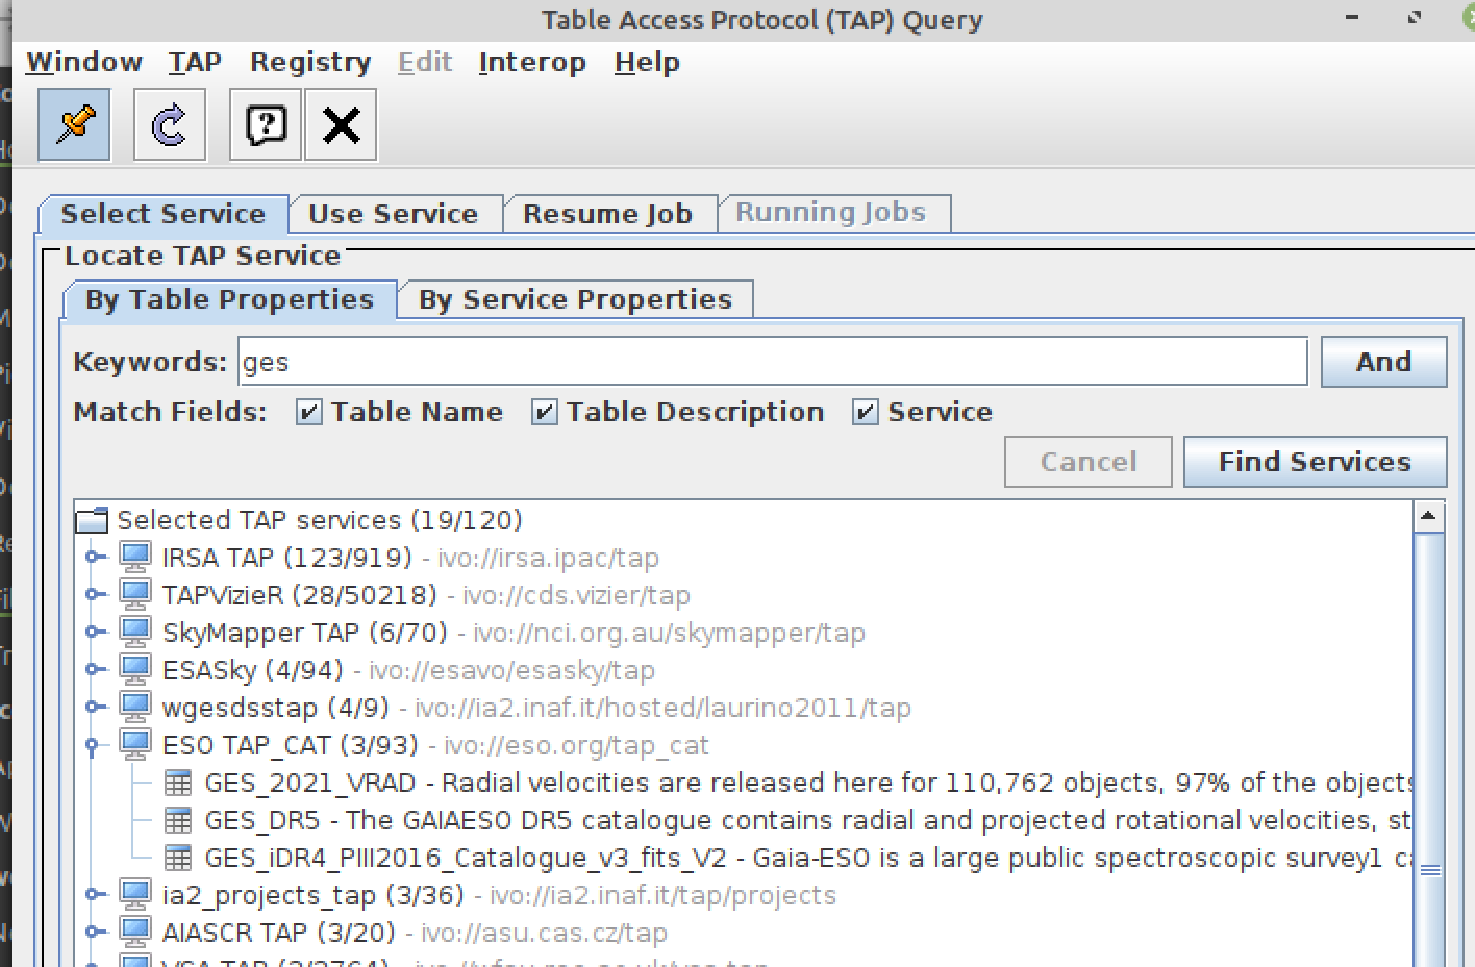
\includegraphics[width=0.7\textwidth]{img/tesis/tap_ges_service.pdf}
	\caption{Búsqueda de catálogos con información de GES. Mediante el uso de TAP, TOPCAT es capaz de ofrecer una lista de catálogos que poseen información referente a GES. En nuestro caso, hemos seleccionado el catálogo publicado por la ESO.}
	\label{fig:tap_ges_service}
\end{figure}


Un ejemplo similar, pero esta vez orientado a localizar catálogos con información de cúmulos abiertos es el que nos ofrece la Figura \ref{fig:tap_query_oc}. Una vez seleccionado el catálogo, TOPCAT nos ofrece la posibilidad de obtener detalles adicionales sobre los esquemas y tablas que los conforman. Esta información es muy útil a la hora de realizar nuestras consultas, ya que de ella podemos extraer no solo las columnas incluidas en la diferentes tablas, sino también el tipo de información que contiene (necesario cuando el nombre de la columna no es suficientemente explicativo), tipo de datos (numérico, texto, fecha...), columnas claves, referencia entre tablas (claves foráneas), y más información relevante. Este conjunto de información adicional es lo que se conoce como meta-información o meta-datos asociados a la tabla (ver Figura \ref{fig:tap_table_metadata}).\par


\begin{figure}
	\centering
	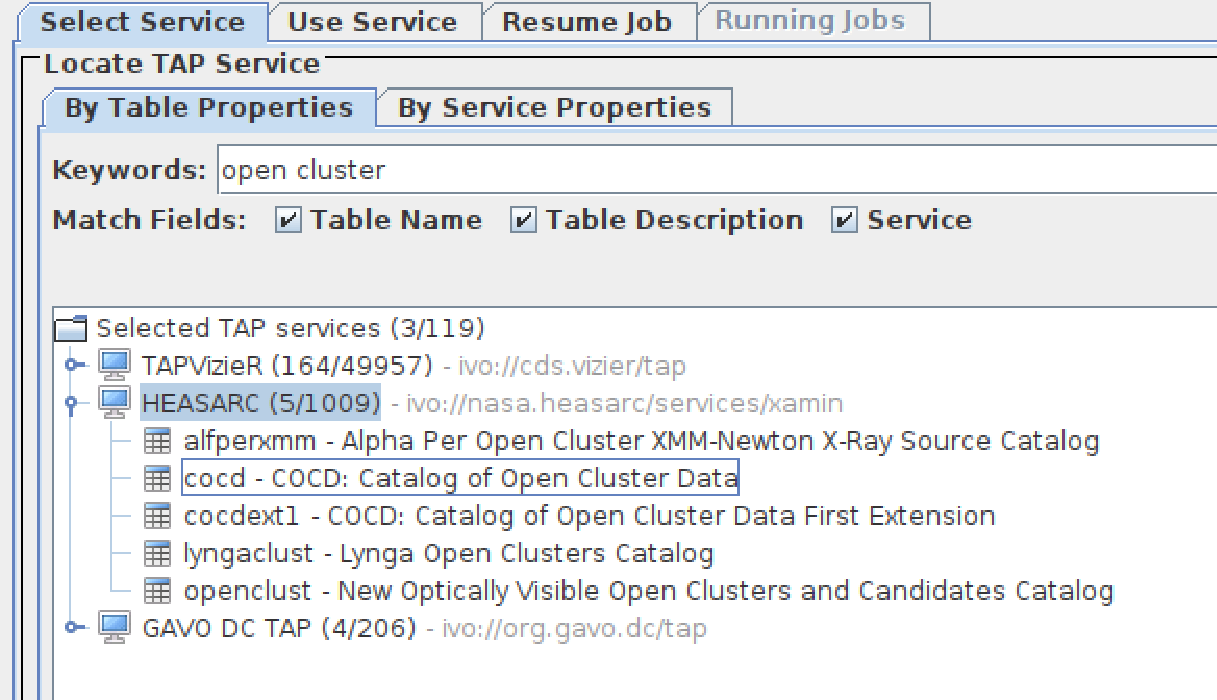
\includegraphics[width=0.7\textwidth]{img/tesis/tap_service.pdf}
	\caption{Búsqueda de catálogos con información relacionada con cúmulos abiertos.}
	\label{fig:tap_query_oc}
\end{figure}

\begin{figure}
	\centering
	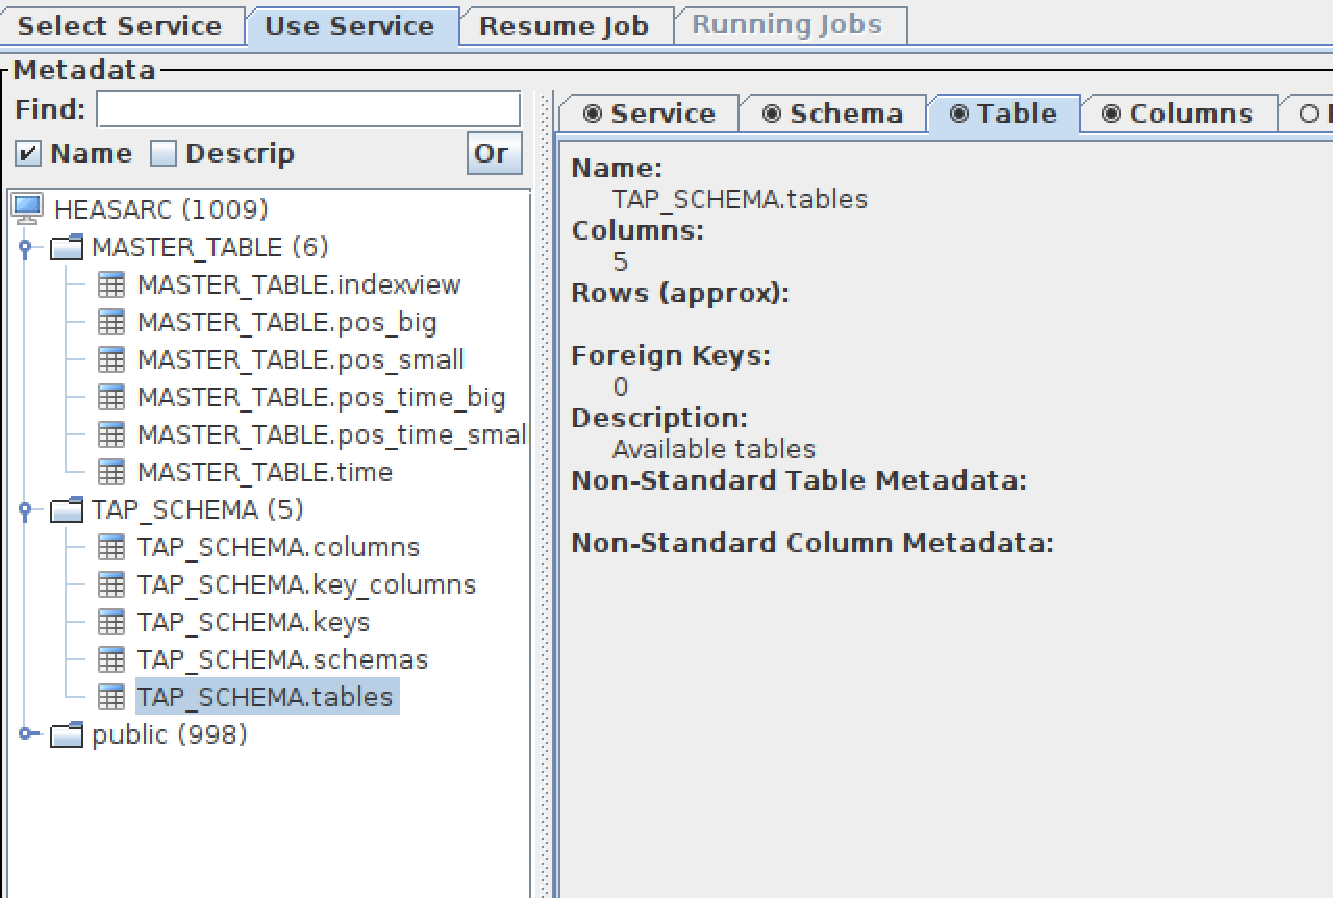
\includegraphics[width=0.7\textwidth]{img/tesis/tap_schema.pdf}
	\caption{Vista con meta-información asociada a una tabla.}
	\label{fig:tap_table_metadata}
\end{figure}

TOPCAT también es capaz de mostrar las diferentes tablas contenidas dentro de un esquema. Un esquema define cómo se organizan los datos dentro, las tablas que los contienen. Esto incluye restricciones lógicas, como nombres de tablas, campos, tipos de datos y las relaciones existente entre ellas (ver Figura \ref{fig:tap_schema_detail}).\par

\begin{figure}
	\centering
	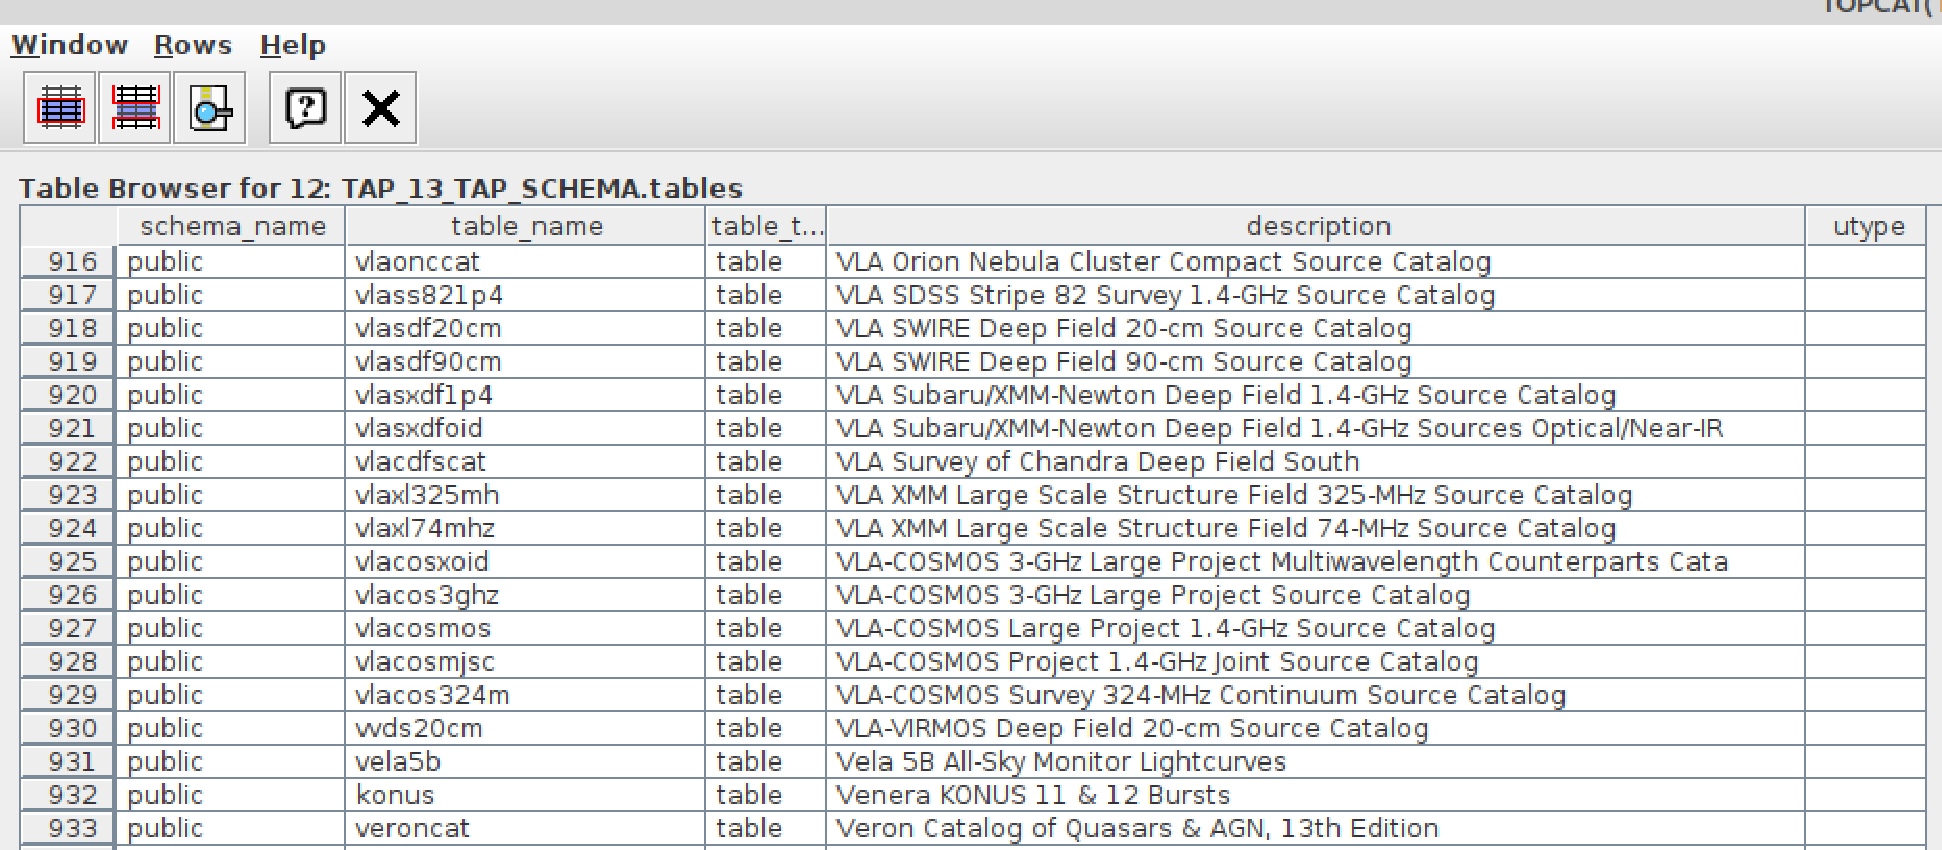
\includegraphics[width=0.7\textwidth]{img/tesis/tap_schema_detail.pdf}
	\caption{Vista con lista de tablas contenida en un esquema.}
	\label{fig:tap_schema_detail}
\end{figure}


\section{Selección de datos}
\subsection{El binomio Gaia-GES}
La combinación de los datos de los catálogos Gaia y GES puede proporcionar una visión completa de las propiedades y evolución de las estrellas similares al Sol. El catálogo Gaia proporciona datos de posición precisos y paralajes, mientras que la GES ofrece información espectroscópica detallada. Esta combinación permite una comprensión más completa de estas estrellas, incluyendo su cinemática, composiciones químicas y potencial para albergar planetas. Al proporcionar una perspectiva más amplia y detallada de estas estrellas, podemos obtener una comprensión más profunda de las propiedades y evolución de las estrellas similares al Sol, lo que representa una fuente de información que se antoja invaluable para la investigación en astrofísica. Estamos ante un conjunto de herramientas poderoso para cualquier astrofísico que estudie estrellas similares al Sol.\par

En el caso de las abundancias de litio, y como ya hemos apuntado, éste es un elemento clave en el estudio de la astrofísica estelar, ya que su abundancia puede proporcionar información valiosa sobre la edad y la historia de las estrellas. Sin embargo, la determinación precisa de las abundancias de litio puede ser un desafío debido a la complejidad de las líneas espectrales de este elemento. GES nos asiste en nuestra investigación aportando su análisis especializado y dedicado de estrellas de todos los tipos espectrales, convirtiéndose así en una herramienta fundamental a la hora de afrontar este desafío.\par

Por otra parte, tenemos información precisa sobre la velocidad angular de las estrellas. Gaia es capaz de medir la velocidad angular de las mismas con una precisión sin precedentes, y ésta nos aporta información crucial para estudiar y entender su rotación, evolución y estructura interna. Combinado esta información con las abundancias de litio podemos establecer hipótesis y validar las mismas acerca del impacto de la velocidad angular sobre este elemento. Paralelamente, la velocidad angular juega un papel crucial en el análisis de la presencia e intensidad de un campo magnético en las estrellas. Los campos magnéticos son responsables de la pérdida de momento angular en las estrellas jóvenes y son la principal fuente de energía detrás de una amplia gama de fenómenos dinámicos (llamaradas, emisión de rayos X, manchas estelares) que ocurren en las capas superficiales del Sol y otras estrellas. Por lo tanto, la medición precisa de la velocidad angular de una estrella puede proporcionar información valiosa sobre la presencia e intensidad de su campo magnético.\par

Otra fuente de información valiosa para nuestra investigación procedente de ambos catálogos es la referida a los cúmulos abiertos. Los cúmulos abiertos son grupos de estrellas que se formaron a partir de la misma nube de gas y polvo. Por lo tanto, todas las estrellas de un cúmulo abierto tienen aproximadamente la misma edad y composición química inicial. Esto los convierte en laboratorios naturales para estudiar la evolución de las estrellas a través de sus diferentes etapas. Gaia ha observado una gran cantidad de cúmulos abiertos, proporcionando datos detallados sobre sus miembros. En paralelo, GES también ha observado un gran número de ellos en un rango amplio de edades. La combinación de ambas fuentes permite estudiar la estructura y dinámica de este tipo de cúmulos, y usarlos para restringir y mejorar los modelos de evolución estelar, algo que hemos puesto en práctica en nuestra investigación.\par

Como acabamos de adelantar, la investigación de los campos magnéticos en estrellas similares al Sol, y en particular de aquéllas que se encuentran en cúmulos abiertos, se beneficia enormemente de los datos proporcionados por ambos catálogos. Los campos magnéticos juegan un papel importante en todas las etapas de la evolución estelar. En estrellas similares al Sol se generan en las capas convectivas exteriores. Estudiar los campos magnéticos a gran escala de estas estrellas puede mejorar nuestra comprensión sobre los mismos y proporcionar restricciones observacionales para los modelos que estudian cómo se generan, la topología que presentan y sus intensidades. Los datos de los catálogos nos asisten a la hora de identificar y estudiar las estrellas con alta actividad magnética, lo que puede proporcionar pistas sobre la dinámica interna de las mismas y su evolución. Combinando esta información con la velocidad angular, nos puede proporcionar indicios de cómo se interrelacionan ambos fenómenos. Adicionalmente, cruzando estos datos con la información de los cúmulos abiertos, obtenemos una visión más clara de cómo los campos magnéticos varían entre las estrellas de la misma edad y composición química.\par


\subsection{Selección de parámetros}
Como indica su nombre, GES pretende complementar los datos sobre paralajes y movimientos propios del satélite Gaia con información extremadamente precisa sobre velocidades radiales (Radial Velocity, RV), litio y química en general. La primera publicación de datos de Gaia (GDR1) \citep{Brown2016} data de 2016 y contiene información sobre los primeros 14 meses funcionamiento de la misión. La segunda publicación de datos de Gaia (GDR2) \citep{Brown2018} publicada en 2018, contiene posiciones, paralajes y movimientos propios de unos 1 300 millones de fuentes, junto con información fotométrica. La tercera publicación de datos de Gaia, la Gaia Early Data Release 3 (GEDR3) \citep{Brown2021} y la Gaia Data Release 3 (GDR3) \citep{Brown2022}, aportan medidas actualizadas y más precisas. GES las mejora y en su última versión (DR5.0) incluye todos los parámetros astrofísicos derivados por el consorcio Gaia-ESO \citep{Gilmore2022}. De interés para nuestra línea de investigación son:
\begin{itemize}
	\item Velocidades radiales y proyectadas
	\item Parámetros estelares (temperatura efectiva, gravedad superficial y metalicidad)
	\item Abundancias de varios elementos, entre ellos el litio
	\item Parámetros específicos para rastrear la acreción y la actividad en estrellas jóvenes
	\item Probabilidad de pertenencia a cúmulos
\end{itemize}


\subsection{Selección de cúmulos abiertos}
GES DR5.0 proporciona información sobre 114 324 estrellas véase \citep[véase][para más detalles]{Gilmore2022}. Para nuestra investigación estamos interesados en considerar aquéllas que pertenecen a OCs, para ello seleccionamos aquellos registros GES que cumplen alguna de las siguientes condiciones:

\begin{itemize}
	\item GE\_CL: observado por GES, campo del programa OC
	\item GE\_SD\_OC: observado por GES, campo estándar OC
	\item AR\_CL: Observación del Archivo ESO, campo de programa OC
	\item AR\_SD\_OC: Observación de archivo, campo estándar OC
\end{itemize}
	
Como resultado de este primer filtrado, el número de registros seleccionados se reduce a 43 299. Sobre este subconjunto de datos realizamos otro filtrado, esta vez dirigido a seleccionar aquellos que ofrecen información no nula sobre los siguientes atributos:

\begin{itemize}
	\item Metalicidad
	\item Abundancia de litio
	\item Identificador de campo GES
	\item Temperatura efectiva
	\item Gravedad superficial
	\item Probabilidad de pertenencia a un cúmulo (>= 0.95\%)
\end{itemize}

Este segundo filtrado reduce la población de estrellas a considerar a un total de 5 895 registros que se distribuyen entre los 64 OCs listados en la Tabla \ref{tab:oc_full_list}.\par

Como datos de referencia tomamos un subconjunto de las observaciones obtenidas por GES. Este subconjunto consiste en aquellas estrellas que pertenecen a OCs, y entre ellas se encuentran potenciales gemelas "ocultas" de nuestro Sol. Para identificar estas últimas, procedemos a realizar una selección adicional, esta vez utilizando los valores dados por nuestros modelos durante las simulaciones para la metalicidad ($\feh$), la temperatura efectiva ($\teff$) y la gravedad superficial ($\gsurf$). Por último, nos quedan las estrellas para las que las observaciones de GES han medido valores congruentes con los resultados de nuestros modelos, a partir de los cuales obtenemos finalmente sus abundancias de litio.\par

\subsection{Selección de gemelos solares} \label{sec:gemelos_solares}
Una vez preseleccionadas las estrellas pertenecientes a los OCs, el interés se centra en identificar las más parecidas a nuestro Sol, es decir, las gemelas solares. Esto nos lleva a preguntarnos qué parámetros estelares debemos tener en cuenta para clasificar una estrella como gemela solar. Encontrarlos nos ayudaría a averiguar el origen de nuestro Sol y a obtener información sobre las condiciones que prevalecían en los OC en los que nacieron.\par

Ya se han realizado varios intentos de encontrar hermanos y gemelos solares. Los primeros se refieren a estrellas que se formaron en el mismo cúmulo que el Sol y, por tanto, deberían tener edades y abundancias químicas muy similares a las de éste \citep[ver][y referencias en él]{Adibekyan2018}. Por otro lado, según \cite{Strobel1996}, se consideran gemelos solares a aquellas estrellas que poseen parámetros físicos fundamentales como $\teff$, $\gsurf$, $\feh$, propiedades fotométricas, composición química, edad, luminosidad, rotación y campos magnéticos similares, si no idénticos, a los del Sol. Localizar estos gemelos solares supone un reto formidable debido a los estrictos criterios y a su dispersión por toda la Vía Láctea.\par 

No es de extrañar que los métodos de búsqueda aplicados se orienten a encontrar las candidatas basándose en sus propiedades cinemáticas. Luego se comparan sus temperaturas, metalicidades y abundancias químicas con las de nuestro Sol. En nuestro estudio, ampliamos los criterios de selección añadiendo la gravedad superficial y la edad de la estrella. Estos dos nuevos parámetros representan un ajuste fino del proceso de búsqueda de candidatos a gemelos. Los catálogos Gaia y GES no proporcionan la edad estimada de los OCs, así que necesitamos recurrir a los resultados obtenidos en el trabajo de \cite{Bragaglia2022} (ver Figura \ref{fig:open_cluster_sample}). Utilizamos la edad de los OCs indicada en la tabla \ref{tab:oc_reduced_list} y los datos obtenidos a partir del conjunto de simulaciones MESA iniciadas con diferentes $\omegaini$, donde $\omegaini = \oomegac$, $\Omega$ es la velocidad angular de la estrella en la superficie estelar, y $\omegac$ es la velocidad superficial en el ecuador de una estrella en rotación donde la fuerza centrífuga equilibra la gravedad newtoniana. La edad derivada de estas simulaciones proporciona un parámetro clave para nuestro análisis. Esta información nos permite determinar los demás parámetros de simulación, que posteriormente utilizaremos para compararlos con los valores asociados a las estrellas pertenecientes a los OCs preseleccionados.\par

\begin{table}
	\centering
	\begin{tabular}{ll} 
		\hline
		Parámetro estelar & Intervalo de selección\\
		\hline
		Edad OC & $\pm0.1\%$ \, para edad < 1 Ga \\
		& $\pm0.15\%$ \, para edad $\geq$ 1 Ga \\
		$\teff$ & $\pm 50.0 \, \Kelvin$ \\
		$\gsurf$ & $\pm 0.05 \, \dex$\\
		$\feh$ & $\pm 0.05 \, \dex$\\
		\hline
	\end{tabular}
	\caption{Parámetros e intervalos de selección aplicados durante el proceso de triaje sobre los componentes del OC.}
	\label{tab:sel_params}
\end{table}

De las aproximadamente 5 900 estrellas identificadas, seleccionamos aquellas cuyos valores de $\feh$, $\teff$ y $\gsurf$ se encuentran en los intervalos correspondientes definidos en la Tabla \ref{tab:sel_params} y según el siguiente proceso de filtrado: a partir de los valores dados por nuestras simulaciones para los parámetros listados en la Tabla \ref{tab:sel_params}, procedemos a seleccionar de los distintos OCs aquellas estrellas que tienen valores dentro de los intervalos establecidos. En concreto, para la edad estimada de un determinado cúmulo, establecemos un intervalo de $\pm$0.1 para OCs jóvenes (edad < 1 Ga) y $\pm$0.15 para contrapartes más viejas (edad >= 1 Ga) \citep{Cantat-Gaudin2020}[véase][para más detalle sobre los valores referidos]. Este intervalo dependiente de la edad sirve como base para seleccionar los pasos de tiempo de simulación que se alinean con los límites de edad inferior y superior de cada grupo. Una vez encontrados estos dos pasos temporales, se reúnen los valores límite asociados para $\teff$, $\gsurf$ y $\feh$. Con estos rangos de valores procedemos entonces a seleccionar en cada uno de los OCs aquellas estrellas que tienen valores para estos mismos parámetros dentro de ellos. De esta forma obtenemos finalmente las estrellas candidatas a ser comparadas con los resultados de la simulación.\par

El resultado del proceso de filtrado puede observarse en las siguientes tablas. En la Tabla \ref{tab:oc_reduced_list} se agrupan los OCs que han aportado alguno de sus miembros en las simulaciones que hemos realizado. Para un determinado OC se informa del número de estrellas que se han seleccionado en las diferentes simulaciones. Por otra parte, las tablas \ref{tab:oc_m67} y \ref{tab:oc_ngc2516} resumen el subconjunto de componentes de los OCs M67 y NGC2516 seleccionados durante las simulaciones para modelos inicializados con $\omegaini = 0.14$. Cada una de las tablas enumera el identificador GES de la estrella y los rangos de $\teff$, $\gsurf$, $\feh$, A(Li), el error estimado de la A(Li) y edad estimada utilizados en la simulación. Estos valores representan los rangos de valores en los que se ha basado el filtrado.


\newpage
\KOMAoptions{paper=landscape,pagesize}
\recalctypearea

\begin{longtable}[c]{|l l l l || c c c c c c c c c c|}
	\hline
	& & & & & & & & $\omegaini$ & & & & & \\
	Cúmulo Abierto & Edad(Ga) & [Fe/H] & $N_*$ & 0.095 & 0.10 & 0.105 & 0.11 & 0.115 & 0.12 & 0.125 & 0.13 & 0.14 & 0.1425\\
	\hline
	Berkeley 21 & 2.138 & -0.21 & 744 & 0 & 0 & 0 & 0 & 0 & 1 & 1 & 1 & 1 & 1\\
	Berkeley 39 & 5.623 & -0.14 & 899 & 1 & 1 & 1 & 1 & 1 & 1 & 2 & 2 & 2 & 2\\
	IC 2602 & 0.036 & -0.06 & 1836 & 0 & 0 & 0 & 0 & 0 & 0 & 1 & 1 & 0 & 0\\
	IC 4665 & 0.033 & 0.01 & 567 & 0 & 0 & 0 & 0 & 1 & 1 & 0 & 0 & 0 & 0\\
	Messier 67 & 3.981 & -0.02 & 131 & 6 & 6 & 6 & 6 & 6 & 6 & 6 & 6 & 6 & 6\\
	NGC 2141 & 1.862 & -0.04 & 853 & 1 & 1 & 1 & 1 & 1 & 1 & 1 & 1 & 1 & 1\\
	NGC 2355 & 1 & -0.13 & 208 & 1 & 1 & 1 & 1 & 1 & 1 & 1 & 1 & 1 & 1\\
	NGC 2420 & 1.698 & -0.15 & 562 & 1 & 1 & 1 & 1 & 1 & 1 & 1 & 1 & 1 & 1\\
	NGC 2425 & 2.399 & -0.13 & 528 & 1 & 1 & 1 & 1 & 1 & 1 & 1 & 1 & 1 & 1\\
	NGC 2451 & 0.035 & -0.08 & 1656 & 0 & 0 & 0 & 0 & 0 & 1 & 1 & 0 & 2 & 1\\
	NGC 2516 & 0.24 & -0.04 & 759 & 0 & 0 & 0 & 1 & 1 & 1 & 3 & 4 & 4 & 3\\
	NGC 3532 & 0.398 & -0.01 & 1145 & 1 & 1 & 0 & 1 & 1 & 1 & 1 & 1 & 0 & 1\\
	NGC 6005 & 1.259 & 0.22 & 560 & 0 & 0 & 0 & 0 & 0 & 0 & 0 & 1 & 1 & 1\\
	NGC 6259 & 0.269 & 0.18 & 494 & 0 & 0 & 0 & 0 & 0 & 0 & 0 & 0 & 0 & 1\\
	NGC 6281 & 0.513 & -0.04 & 320 & 0 & 0 & 0 & 0 & 0 & 0 & 0 & 0 & 1 & 1\\
	NGC 6405 & 0.035 & -0.02 & 701 & 1 & 1 & 1 & 0 & 1 & 3 & 2 & 0 & 0 & 0\\
	NGC 6633 & 0.692 & -0.03 & 1662 & 2 & 2 & 2 & 1 & 1 & 0 & 0 & 0 & 1 & 1\\
	NGC 6709 & 0.191 & -0.02 & 730 & 2 & 1 & 0 & 0 & 0 & 0 & 0 & 0 & 1 & 1\\
	Trumpler 20 & 1.862 & 0.13 & 1213 & 3 & 3 & 3 & 2 & 2 & 2 & 2 & 2 & 2 & 2\\
	\hline
	\caption{Lista de los OCs seleccionados. Para cada OC se indica el nombre, la edad estimada, la metalicidad y el número de componentes. Además, se muestran los diferentes $\omegaini$ utilizados en las distintas simulaciones, donde $\omegaini = \oomegac$, $\Omega$ es la velocidad angular de la estrella en la superficie estelar, y $\omegac$ es la velocidad superficial en el ecuador de una estrella en rotación donde la fuerza centrífuga equilibra la gravedad newtoniana. Para cada entrada del OC se informa por $\omegaini$ de cuántos componentes del OC cuyos parámetros estelares, tras compararlos con los equivalentes calculados por las simulaciones, se seleccionan. Los componentes OC seleccionados se utilizan como referencia en las figuras que se muestran en las secciones siguientes.}
	\label{tab:oc_reduced_list}	
\end{longtable}
\newpage
\KOMAoptions{paper=portrait,pagesize}
\recalctypearea


\begin{table}
	\centering
	\begin{tabular}{l l l l l l l} 
		\hline
		Id Objeto & $\teff$(K) & $\gsurf$(dex) & FeH(dex) & ALi(dex) & eALi(dex) & Edad(Ga)\\
		\hline
		8510914-1157003 & 5843 & 4.42 & -0.03 & 1.8 & 0.08 & 3.981\\ 
		8510991-1146169 & 5797 & 4.4 & -0.01 & 1.65 & 0.08 & 3.981\\ 
		8512177-1144050 & 5818 & 4.46 & 0 & 1.99 & 0.06 & 3.981\\ 
		8513941-1200571 & 5792 & 4.41 & -0.02 & 1.49 & 0.13 & 3.981\\ 
		8515559-1148381 & 5794 & 4.43 & -0.04 & 1.56 & 0.1 & 3.981\\ 
		8520350-1147480 & 5875 & 4.47 & -0.03 & 1.21 & 0.24 & 3.981\\ 
		\hline
	\end{tabular}
	\caption{M67 - Configuración de filtro: Identificador estelar GES, $\teff$(K) [5787.4892, 5887.6823], $\gsurf$(dex) [4.3979, 4.4977], $\feh$(dex) [-0.05, 0.05], Edad(Ga) [3.977, 3.985]}
	\label{tab:oc_m67}
\end{table}

\begin{table}
	\centering
	\begin{tabular}{l l l l l l l} 
		\hline
		Id Objeto & $\teff$(K) & $\gsurf$(dex) & FeH(dex) & ALi(dex) & eALi(dex) & Edad(Ga)\\
		\hline
		7571111-6048156 & 5084 & 4.54 & 0 & 2.29 & 0.08 & 0.24\\ 
		7595031-6044149 & 5108 & 4.52 & -0.05 & 1.92 & 0.08 & 0.24\\ 
		7595280-6032498 & 5093 & 4.49 & -0.03 & 2.29 & 0.08 & 0.24\\ 
		\hline
	\end{tabular}
	\caption{NGC2516 - Configuración de filtro: Identificador estelar GES, $\teff$(K) [5010.0324, 5111.0095], $\gsurf$(dex) [4.4405, 4.5405], $\feh$(dex) [-0.05, 0.05], Edad(Ga) [0.23964, 0.24036]}
	\label{tab:oc_ngc2516}
\end{table}



\begin{figure}
	\centering
	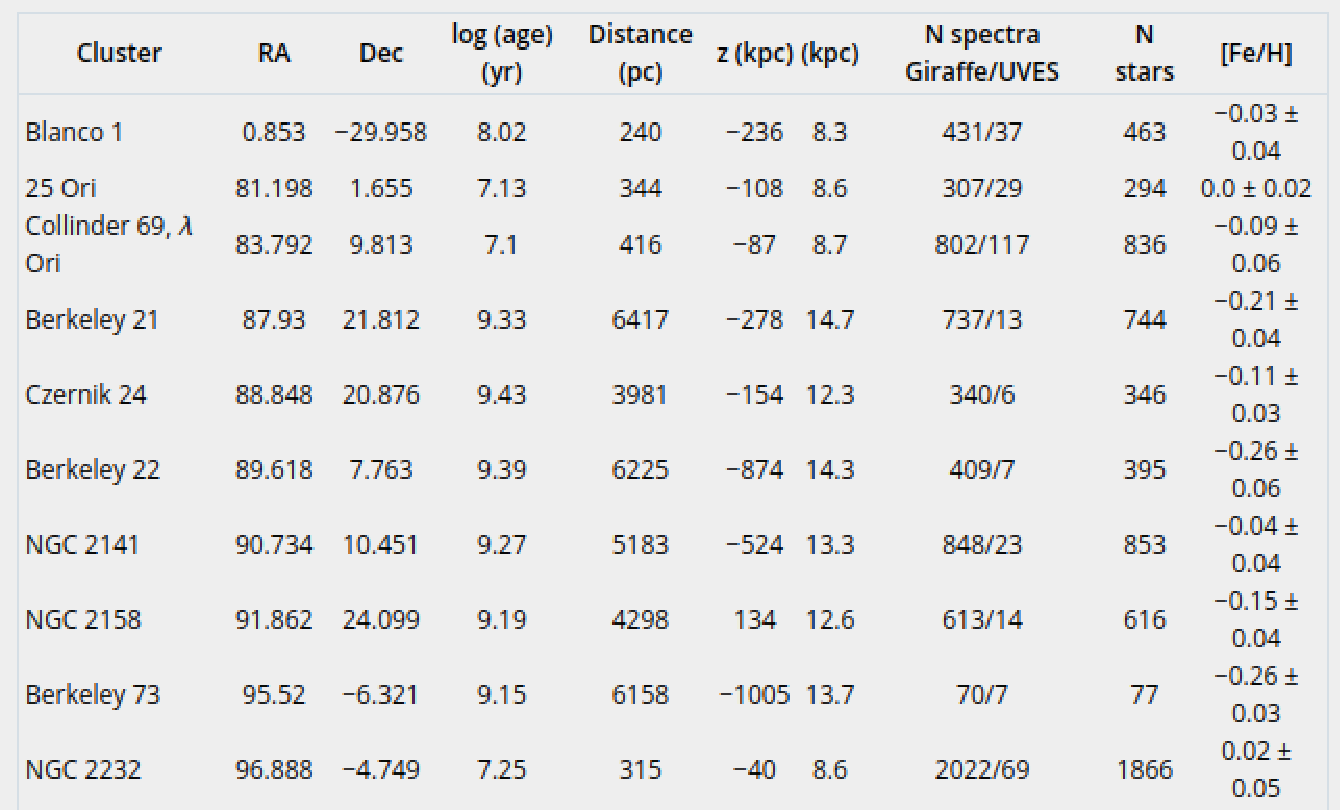
\includegraphics[width=0.7\textwidth]{img/tesis/open_cluster_sample.pdf}
	\caption{Tabla obtenida de \cite{Bragaglia2022}. Las columnas 1 a 7 listan la denominación del cúmulo, las coordenadas de ascensión recta y declinación, la edad estimada del cúmulo, la distancia (módulo de distancia convertido) en parsecs (pc) , la posición Z en coordenadas cartesianas galácticas, y la distancia desde el centro galáctico suponiendo que el Sol está a 8340 pc. Las columnas 8 y 9 enumeran el número de espectros y objetivos, mientras que la media de [Fe/H] y la desviación estándar se dan en la columna 10.}
	\label{fig:open_cluster_sample}
\end{figure}


\endinput
%--------------------------------------------------------------------
% FIN DEL CAPÍTULO. 
%--------------------------------------------------------------------


\cleardoublepage
\part{Rotación y campos magnéticos de intensidad fija}
% !TeX root = ../libro.tex
% !TeX encoding = utf8

\chapter{Rotación y campos magnéticos de intensidad constante}\label{ch:tercer-capitulo}

\section{Introducción}

El impacto de la rotación tanto en la PMS como en el agotamiento del Li para las estrellas de tipo solar ha sido ampliamente debatido en el pasado \cite{Pinsonneault1997,Jeffries2004,Somers2014} y revisado más recientemente sobre la base de la disponibilidad de medidas más precisas \cite{Bouvier2016}. Sin embargo, estos estudios previos se centraron principalmente en los efectos hidrostáticos y no consideraron la influencia de un acoplamiento entre el campo magnético estelar y su posible efecto de desacelaración. Se piensa que la AML tiene una influencia directa en los procesos de mezcla y que el transporte del momento podría producirse por una serie de mecanismos tales como: pérdida de masa, campos magnéticos y ondas gravitatorias (modos g). Respecto a estos dos últimos, las ondas gravitatorias \cite{Charbonnel2005, Pincon2016} y los campos magnéticos \cite{Eggenberger2009} tienen la propiedad de transmitir el momento angular (AM) de forma mucho más eficaz que inducir la mezcla \cite{Denissenkov2007}. Como consecuencia de este incremento en la eficiencia del transporte del AM, se reduce la cantidad de rotación diferencial entre las zonas radiativa y convectiva de la estrella (se fomenta una rotación de cuerpo sólido), así como las inestabilidades rotacionales inducidas. Además, también se originarían campos magnéticos en los límites entre estas zonas, en las llamadas tacoclinas \cite{Aschwanden2014, Guerrero2016}, que interaccionarían con las partículas del viento solar que se verían obligadas a rotar en sincronía con el campo magnético imperante y por tanto, frenarían la rotación estrella. Esto es lo que se conoce como el efecto de frenado magnético (Magnetic Braking, MB). \par

\begin{figure}
    \centering
    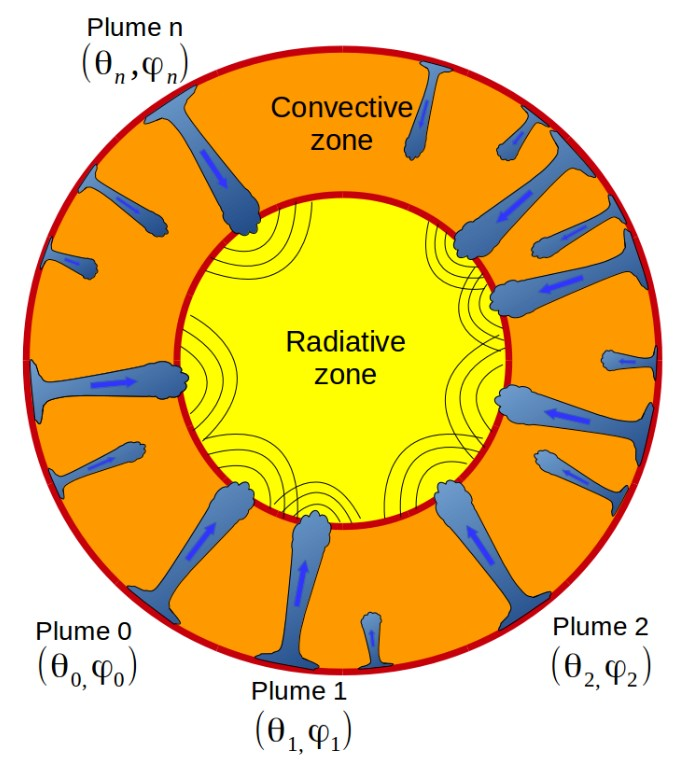
\includegraphics[width=0.5\textwidth]{img/tesis/gravitational_waves.jpg}
    \caption{Vista esquemática de la estrella. Los penachos convectivos se producen en las capas superiores de la estrella y se adentran en la región convectiva. Crecen por arrastre turbulento de materia en sus bordes y alcanzan la parte superior de la zona radiativa. Allí, cada una de ellas, caracterizada por su posición angular ($\theta_i$,$\phi_i$), libera una parte de su energía cinética y genera ondas internas que pueden propagarse hacia el centro. (Figura tomada de \cite{Pincon2016})}
    \label{fig:grav_waves}
\end{figure}

A día de hoy, los modelos estándar no son capaces de replicar de forma satisfactoria los valores observados de abundancia de Li en las superficies estelares con las predicciones que estos modelos arrojan. Esta falta de concordancia nos hace pensar que ciertos mecanismos físicos que influyen en la destrucción del Li están siendo modelizados de forma inadecuada o simplemente no se tienen en cuenta, como por ejemplo el frenado magnético. A la vista de estos hallazgos, parece evidente que aún quedan cuestiones abiertas por resolver sobre el tema de los procesos que participan, directa o indirectamente, en los mecanismos de mezcla que no están incorporados en los modelos estelares estándar. Por ello, es imprescindible una adecuada consideración de las interacciones entre rotación y campos magnéticos a la hora de estudiar la distribución del AM. \par

La abundancia de Li observada en la fotosfera de las estrellas es un indicador de su composición interior y de los procesos de mezclado que en su interior tienen lugar. Adicionalmente, estas abundancias (además de otras métricas) se utilizan para comprobar la validez de los modelos estelares. Para que esto sea posible hay que tomar como premisa inicial que la abundancia de Li generada en la nucleosíntesis asociada al Big Bang es conocida y este elemento solo se destruye a través de reacciones nucleares. A pesar de décadas de esfuerzos teóricos, se sigue sin encontrar una explicación coherente con los modelos para las discrepancias encontradas en las comparaciones sobre la abundancia de Li para estrellas pertenecientes a cúmulos de diferentes edades y que se encuentran en el mismo estado evolutivo, o bien en la PMS, o bien en MS. Los modelos no son capaces de explicar las abundancias detectadas en las etapas tardías de la MS \cite{Tschape2001}.\par

Es sabido que parte de la pérdida de Li se produce durante la PMS y que además ésta se acentúa según decrece la masa de la estrella y, a igualdad de masa, según aumenta la metalicidad de la misma. Para reproducir la dependencia entre la edad y masa de las estrellas con la merma de las concentraciones de Li, estos modelos necesitan de una combinación de procesos de mezclado cada vez más complejos, como overshooting, mezclado debido a procesos rotacionales o difusión microscópica.
Para las estrellas de tipo solar, nos encontramos con dos factores que tienen que ser explicados desde el punto de vista de la abundancia de Li:

\begin{enumerate}
    \item La deficiencia generalizada de Li en el Sol y en estrellas de tipo tardío presentes en cúmulos a diferentes edades.
    \item La gran dispersión en abundancia de Li que existe en estrellas con una determinada temperatura efectiva detectada en los cúmulos abiertos.
\end{enumerate}

Existen datos observacionales que sugieren que las estrellas que giran más rápido preservan el Li mejor que las que lo hacen más lentamente. Este hecho se puede deber a que por encima de cierto umbral de velocidad de rotación, ésta impide de manera drástica la penetración vertical de penachos generados por movimientos convectivos que, cuando están presentes, contribuyen a hacer más eficiente el proceso de destrucción de Li \cite{Baraffe2017}.\par

Adicionalmente y según el modelo estándar de nucleosíntesis para el Big Bang, la abundancia de Li original puede estimarse en 2.6 dex \cite{Spergel2003} pero la abundancia de litio detectadas en meteoritos se conoce que está en el orden A(Li) = [3.26-3.34] dex \cite{Randich2006, Grevesse2007}, lo que apunta hacia un enriquecimiento desde que se produjo el Big Bang. Por otro lado, la abundancia medida en las estrellas de tipo solar es del orden de ALi = 1.05 dex \cite{Grevesse2007}, lo que implica la existencia de procesos de destrucción del Li en su interior.  Esta discrepancia entre las abundancias medidas en meteoritos y en estrellas de tipo solar es lo que ha pasado a denominarse el “problema del litio”.\par

Continuando con la importancia del Li y teniendo en cuenta que tanto éste, como los demás elementos ligeros berilio y boro, se queman a temperaturas relativamente bajas en interiores estelares, tenemos que estos elementos sólo sobreviven en las capas más externas de una estrella, donde la temperatura es menor. Adicionalmente, su presencia es un trazador muy potente relacionado con los mecanismos de mezcla en funcionamiento en estructuras estelares, ya que nos puede aportar información acerca de qué tal eficientes son a la hora de transportar estos elementos a zonas más interiores donde serían destruidos.\par

\section{El Sol y la rotación}
Nuestro Sol, como estrella que es y como ocurre con el resto de los cuerpos celestes, gira en torno a su eje. El tiempo que tarda en completar una revolución completa sobre este es de aproximadamente 26 días. Decimos aproximadamente porque la duración del día solar es diferente dependiendo de la latitud que se tome como referencia. Si comparamos las velocidades de rotación solar y la terrestre con respecto al diámetro de los correspondiente cuerpos celestes, se obtiene que un punto situado sobre la superficie solar girar aproximadamente cuatro veces más rápido de lo que lo haría sobre la Tierra.

Esto ocurre porque, a diferencia de la Tierra, el Sol no es un cuerpo rígido. Por lo tanto, al estudiar la rotación del Sol, no se puede considerar como una estructura compacta. El Sol es en realidad una enorme esfera de plasma, más parecida a una enorme bola de gas que a una estructura sólida rígida.\par

Si tomamos como referencia medidas de la rotación solar a lo largo de un período largo de tiempo podemos observar que, dependiendo de la latitud que tomemos como referencia, la velocidad de rotación se va incrementando conforme la distancia al ecuador solar se reduce. Es decir, el Sol gira más rápidamente en el ecuador que en sus polos \ref{fig:rot_solar_vs_latitud}. Este comportamiento que se conoce como rotación diferencial fue descrito por Richard Carrington (1826-1875) tras analizar el movimiento de las manchas solares \cite{Carrington1863}. Carrington dedujo la siguiente ley empírica mediante donde $\Omega_*$ es la cantidad angular de la rotación diaria y $\phi$ es la latitud heliográfica, que corresponde a la latitud en la Tierra  \cite{Banisch2009}.\par

\begin{ceqn}
\begin{equation}
    \Omega_* = 14.4 - 2.8\sin^2\phi \label{eq:ang_rot_sun}
\end{equation}
\end{ceqn}

\begin{figure}
    \centering
    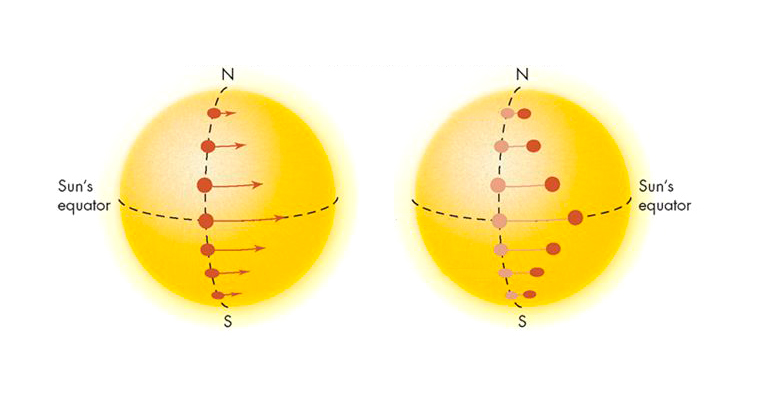
\includegraphics[width=0.8\textwidth]{img/tesis/sun_1.png}
    \caption{Rotación diferencial presente en el Sol. Tomando como referencia un meridiano solar y situando sobre este diferentes puntos de referencias a diferentes latitudes, se observa que la velocidad con la que estos giran es mayor a medida la distancia al ecuador solar disminuye. Crédito McGraw-Hill.}
    \label{fig:rot_solar_vs_latitud}
\end{figure}

El período de rotación $d_*$ en días se calcula como:

\begin{equation}\label{eq:dia_solar}
    d_* = \frac{360}{\Omega_*}
\end{equation}

En la región ecuatorial la rotación dura solo 25 días, mientras que en los polos el Sol gira más lentamente \ref{fig:ang_solar_vs_latitud}. Aquí el día solar tiene una duración aproximada de 30 días. A pesar de esta rotación diferencial entre regiones situadas en latitudes diferentes, no se produce un aplanamiento reseñable del disco solar ya que la velocidad de rotación es pequeña, de media 2km/s \cite{Gill2012}.\par

\begin{figure}
    \centering
    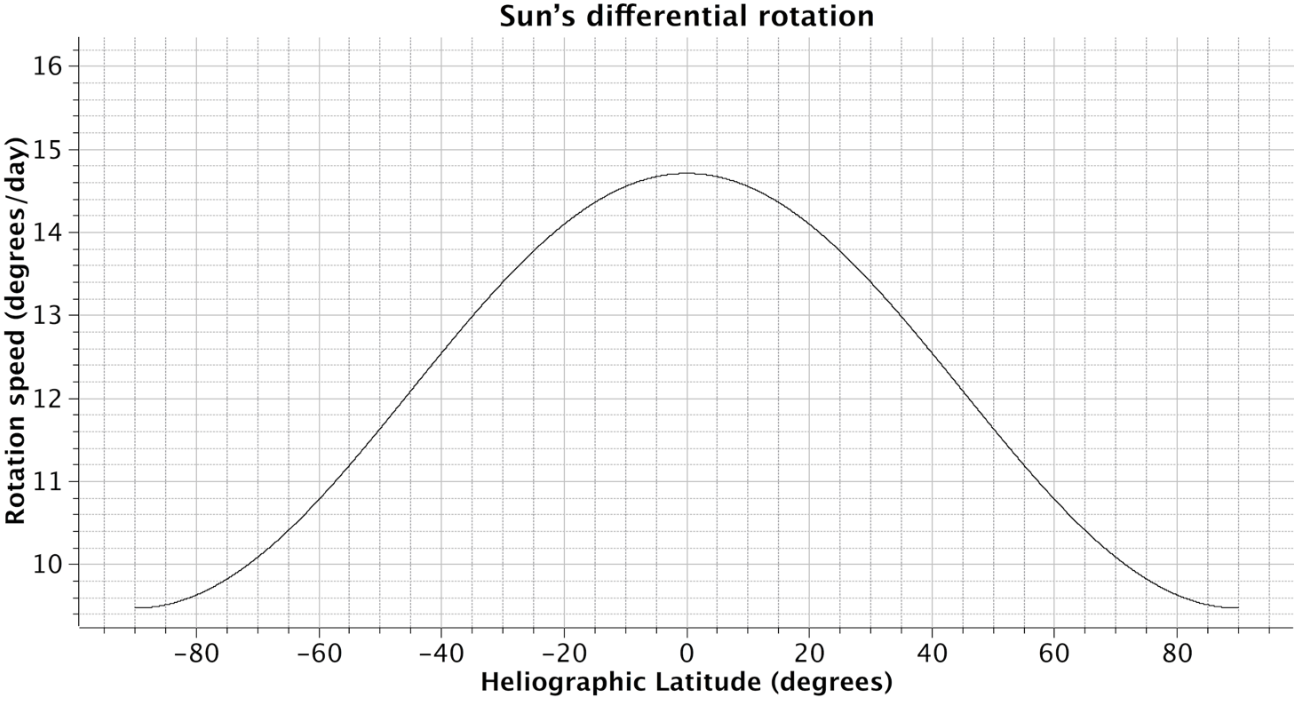
\includegraphics[width=1.0\textwidth]{img/tesis/sun_3.png}
    \caption{Valor predicho teóricamente para la velocidad de rotación del Sol en función de la latitud. Sobre el ecuador solar se obtiene la máxima velocidad angular y esta va disminuyendo a medida que aumenta la latitud. Crédito CESAR ESAC.}
    \label{fig:ang_solar_vs_latitud}
\end{figure}


\section{Efectos de los campos magnéticos}
Aún se desconoce el origen de los campos magnéticos en las estrellas. Los campos magnéticos organizados detectados en algunas estrellas O \cite{Wade2010} podrían ser campos fósiles \cite[ver][para más detalles ]{Dudorov2014}, o campos producidos mediante un mecanismo de dinamo \cite{Cantiello2009}. Además, la presencia de campos magnéticos con intensidades del orden de kG \cite{Hussain2014} ha sido una condición sine qua non para tratar ciertos datos observados en estrellas de tipo T Tauri en sistemas PMS jóvenes en acreción \cite{Johns-Krull2007}.\par

La masa de las estrellas juega un papel determinante en la existencia o no de una envoltura convectiva externa. A su vez, la presencia de esta región convectiva condiciona la evolución de los campos magnéticos. Las estrellas masivas no tienen zonas convectivas externas aunque pueden exponer un núcleo convectivo. En cambio, las estrellas menos masivas, como el Sol, tienen envolturas convectivas y un núcleo radiativo. En ambos tipos de estrellas se pueden generar fuertes campos magnéticos en la tacoclina pero con notables diferencias \cite[v.g.][para más detalles]{Chabrier2006,Charbonneau2010}.\par

En el Sol, la materia que lo compone se encuentra en su mayoría presente en forma de plasma. Es este estado, la envoltura electrónica se encuentra desacoplada del núcleo atómico y bajo ciertas condiciones físicas pueden moverse libremente, por lo que pueden poner en movimiento una carga electrónica. Bajo estas condiciones, la materia solar puede alcanzar la conductividad del cobre \cite{Banisch2009}.\par

\subsection{El mecanismo de dinamo}
Una dinamo es el proceso por el cual la energía mecánica se convierte
convierte en energía electromagnética por inducción. La energía mecánica se debe al movimiento de los fluidos y la energía electromagnética resultante produce los campos magnéticos observados. Para que una estrella tenga un campo magnético generado por dinamo, debe contener una región fluida conductora de electricidad que experimente movimientos para generar inducción. Sin embargo, existen otras condiciones necesarias para el vigor y la morfología de los movimientos que se derivan del hecho de que el campo magnético no debe decaer debido a la disipación óhmica. La necesidad básica para mantener un mecanismo de dinamo es una región fluida eléctricamente conductora en el interior de la estrella.

El Sol se rige por un fuerte campo magnético que se genera con una intensidad de campo magnético de B z 10 5 G \cite{Aschwanden2014} en la tacoclina, la delgada capa de cizalla intercalada entre la zona radiativa y la convectiva. Los tubos de flujo magnético flotante se elevan a través de la zona de convección (debido a la inestabilidad convectiva que obedece a la ley de Schwarz).
que obedece al criterio de Schwarzschild) y emergen en la superficie solar en las regiones activas, donde forman manchas solares con intensidades de campo magnético de B z 10 3 G y bucles coronales con intensidades de campo de B z 10 2 G en los puntos de apoyo fotosféricos, y de B z 10 G en las mayores alturas coronales. Se cree que la rotación diferencial en la superficie solar enrolla el campo magnético superficial, que se fragmenta bajo la tensión magnética, circula meridionalmente hacia los polos y se reorienta desde el estado de tensión toroidal (con líneas de campo orientadas en dirección este-oeste) en el máximo solar a un campo dipolar poloidal (que conecta el polo norte con el polo sur) en el mínimo solar.
mínimo solar.

\subsection{Campos magnéticos internos}
Nuestro Sol es una estrella activa en lo que se refiere al campo magnético. Según los modelos teóricos este campo magnético es generado por una dinamo en la tacoclina y con una intensidad en torno a $B\approx10^{5}\,\Gauss$ \cite{Maeder2003a,Dudorov2014}. En el momento de su generación, las líneas de ese campo magnético tendrán una orientación poloidal y se verán afectadas por la rotación diferencial y obligadas a adoptar una tipología toroidal (el efecto $\omega$). Por otro lado, también puede darse el caso contrario, partiendo de un campo magnético toroidal obtener una configuración poloidal. Esto sería posible gracias a los movimientos convectivos de material que se producen en el CZ de la estrella y suponer que este material se comporta como un conductor perfecto. Esta segunda condición permite suponer que las líneas de campo magnético están "congeladas" en el fluido conductor y por tanto deben moverse solidariamente con él (efecto $\alpha$) \cite{Stanley2014}.\par

\begin{figure}
    \centering
    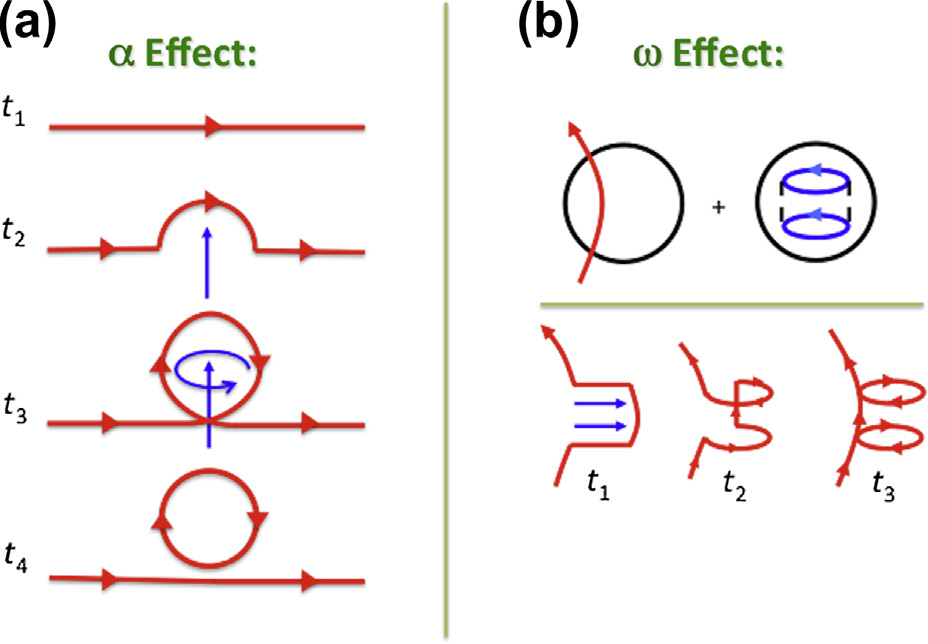
\includegraphics[width=0.6\textwidth]{img/tesis/alpha_omega_effect.png}
    \caption{Esquema de los mecanismos canónicos de generación de dinamo. Las líneas de campo magnético están en rojo y los campos de velocidad en azul. \textbf{(a)} En el efecto, un flujo helicoidal estira ($t_2$) y luego retuerce ($t_3$) el campo magnético. Una pequeña cantidad de difusión en el punto de torsión ($t_4$) puede generar un bucle de campo magnético ortogonal al campo original. \textbf{(b)} En el efecto $\omega$, una rotación diferencial a gran escala afecta una línea de campo poloidal y la estira en dirección zonal ($t_1$ - $t_3$) generando bucles magnéticos toroidales a partir de la línea de campo poloidal. El círculo negro indica el límite exterior de la región de la dinamo. \cite{Stanley2014}}
    \label{fig:alpha_omega_effect}
\end{figure}


\subsection{Campos magnéticos superficiales} \label{surf_mf}
La intensidad del campo magnético medida en la superficie del Sol es de aproximadamente $B\approx1\,\Gauss$ \cite{Weber1967,DAntona2000,Morin2012}, el doble del valor del de la Tierra. Además su topología es variada y compleja. El modelo de dinamo establece que el campo magnético producido en el interior de la estrella alcanza la superficie con la ayuda de procesos convectivos que tienen lugar en la CZ y da lugar a regiones magnéticamente activas en la superficie solar. Además, las estrellas en rotación que exponen una CZ exterior significativa pueden producir campos magnéticos superficiales a través de un mecanismo de dinamo \cite[v.g.][]{Brandenburg2004,Charbonneau2010,Brun2017}. Sea cual sea el origen de los campos magnéticos superficiales, se predice un acoplamiento con el viento estelar, provocando así una pérdida de masa y, si ésta es lo suficientemente fuerte, produzcan MB \cite[v.g.][]{UdDoula2002,Ud-Doula2007,Ud-Doula2008,Meynet2010}.\par


\section{Efectos del frenado magnético - Parte I}
En su enfoque más aceptado, el MB está vinculado al trabajo de Skumanich \cite{Skumanich1972} en el que desarrolla una ley empírica de su evolución en paralelo a la edad de la estrella. Para calibrar esta ley, Skumanich se basó en datos obtenidos de estrellas de tipo G encontradas en la MS. La influencia del MB en la evolución de la estrella está estrechamente relacionada con el transporte del AM. Según \cite{Meynet2010}, se distinguen dos mecanismos principales atendiendo a cómo se produce el transporte del AM:

\begin{enumerate}
    \item Rotación diferencial: el transporte de AM es impulsado por corrientes meridionales e inestabilidades de cizalla.
    \item Rotación de cuerpo sólido: cuando el transporte de AM es muy eficiente, la rotación de cuerpo sólido se mantiene durante toda la MS.
\end{enumerate}

El AML causado por MB depende directamente de la cantidad de masa perdida por la estrella debido a los vientos estelares. El coeficiente de pérdida de masa estimado para una estrella de tipo solar, aproximadamente $10^{-14}\msun \; yr^{-1}$ \cite{Noerdlinger2008}, y el AML resultante derivado de ese valor pueden considerarse relativamente modesto como para influir decisivamente en la evolución de la estrella. Además, el efecto combinado de los movimientos convectivos y la rotación diferencial conducen a la generación de campos magnéticos. Esos campos magnéticos acaban alcanzando la superficie de la estrella, de modo que el AML puede incrementarse en varios órdenes de magnitud \cite{Langer2012}. Ese incremento es consecuencia del campo magnético que obliga a las partículas ionizadas del viento estelar a girar con la misma velocidad angular, vientos que se extienden una distancia varias veces superior al radio de la estrella \cite[ver][para más detalles]{UdDoula2002,Ud-Doula2007,Ud-Doula2008}.

Además, a lo largo de la evolución de la estrella, parámetros directamente observables como su velocidad de rotación, temperatura efectiva, gravedad superficial o abundancia de elementos químicos sufren variaciones. Estos parámetros influyen, directa o indirectamente, en la pérdida de momento angular causada por el campo magnético de la estrella.\par


\subsection{Formalismo de frenado magnético de intesidad fija} \label{mod_mb}
Comenzamos enumerando los aspectos más relevantes y las suposiciones realizadas en la modelización de la evolución de la rotación, el frenado magnético y el momento angular en MESA. Estos serán considerados para el cálculo del AML como resultado del par aplicado por un viento estelar acoplado magnéticamente.\par 

En presencia de pérdida de masa, el material del viento estelar elimina el AM, lo que provoca un efecto de giro a la baja. Esto es muy importante, por ejemplo, en las estrellas masivas, que se sabe que rotan rápidamente y tienen fuertes vientos estelares. También se ha observado que las estrellas de masa intermedia fuertemente magnéticas suelen tener tasas de rotación mucho más lentas que otras estrellas de su población parental \cite{Mathys2006}. En esas estrellas, la presencia de dicho campo magnético interactuará con la pérdida de masa y el radio Alfv'{e}n ($R_{A}$) juega un papel importante en esta interacción.\par

En el resto de este trabajo, describimos dos enfoques semi-empíricos para el cálculo del AML como resultado del par aplicado por un viento estelar acoplado magnéticamente. Esto se ha implementado como una extensión del código de evolución estelar Modules for Experiments in Stellar Astrophysics \cite[MESA; ][]{Paxton2011, Paxton2013,Paxton2015, Paxton2018, Paxton2019}.

\subsubsection{Frenado magnético de intesidad fija según Ud-Doula \& Owocki (2002)}
Un parámetro relevante para caracterizar la influencia de un campo magnético dado sobre el viento estelar es el denominado parámetro magnético de confinamiento del viento ($\eta_*$). Representa una relación energética (Ec.~\ref{eq:wind_conf}) y define un parámetro característico de la eficacia relativa de los campos magnéticos para circunscribir y/o canalizar el flujo de salida del viento \cite{UdDoula2002}.\par

\begin{ceqn}
\begin{equation}
    \eta_* = \frac{B^{2}/8 \pi}{3} \label{eq:wind_conf2}
\end{equation}
\end{ceqn}


\begin{ceqn}
\begin{equation}
    \eta_* = \frac{B^{2}/8\pi}{\rho\nu^2/2} \label{eq:wind_conf}
\end{equation}
\end{ceqn}

donde $B^{2}/8\pi$ es la densidad de energía del campo magnético, $\frac{1}{2}\rho\nu^{2}$ la densidad de energía cinética, $B$ la intensidad del campo magnético, $\rho$ la densidad de masa, y $\nu$ la velocidad del viento estelar.\par

Haciendo uso de $\eta_*$, el $R_{A}$ se define como el punto en el que se equilibran la densidad de energía del campo magnético, marcada $B$, y la densidad de energía cinética, definida por $\rho$ y $(\nu)$. Es decir, donde el coeficiente entre ambos es igual a 1. En caso de que $R_{A}$ sea mayor que el radio de la estrella, entonces el flujo del viento tendrá que seguir el campo magnético. Como consecuencia, el material saldrá de la superficie estelar con un AM específico mayor, ya que el radio de co-rotación ha aumentado y corresponderá aproximadamente al $R_{A}$. Este efecto se conoce como MB.\par

Las estrellas con masas iniciales similares pero diferentes relaciones de pérdida de masa ($\Dot{M}$) acabarán evolucionando de forma muy diferente. Las partículas ionizadas transportadas por el viento solar no sólo contribuyen a la pérdida de masa, sino también a la pérdida de energía cinética que se deposita en el medio interestelar. Dada una estrella con un viento esféricamente simétrico, $\Dot{M}$ se caracteriza por la siguiente expresión:

\begin{ceqn}
\begin{equation}
    \Dot{M} = 4\pi r^2\rho\nu \label{eq:mass_loss}
\end{equation}
\end{ceqn}

Usando (\ref{eq:wind_conf}) and (\ref{eq:mass_loss}), $\eta_*$ puede ser aproximado por: 
\begin{ceqn}
\begin{equation}
    \eta_* = \frac{B^{2}r^{2}}{\Dot{M}\nu} \label{eq:wind_conf2}
\end{equation}
\end{ceqn}

\begin{ceqn}
\begin{align}
    \Dot{M} &= 4\pi r^2\rho\nu \label{eq:mass_loss}\\
    K_e &= 0.5\Dot{M}\nu_{esc}
\end{align}
\end{ceqn}


\begin{ceqn}
\begin{equation}
    \eta_* = \frac{B^{2}r^{2}}{\Dot{M}\nu} \label{eq:wind_conf2}
\end{equation}
\end{ceqn}

\begin{equation}\label{eq:identidad-pitagorica2}
  \cos^2 x + \sin^2 x = 1.
\end{equation}

A su vez, de las características observables del viento solar, nos importan especialmente los parámetros relacionados con la cantidad de masa que es capaz de arrancar de las capas externas de la estrella en un intervalo de tiempo dado, y la velocidad que alcanza el propio viento medida a gran distancia de la estrella, la velocidad terminal ($\nu_\infty$). En general, un flujo de salida canalizado magnéticamente tendrá una geometría de corriente compleja pero, por conveniencia, la Ec.~\ref{eq:mass_loss} simplemente caracteriza la fuerza del viento en términos de una tasa de pérdida de masa distribuida simétricamente sobre una esfera. $\nu$ puede caracterizarse por la variación radial de la velocidad del flujo saliente en términos de la ley de velocidad (Ec.~\ref{eq:vel_law}), donde $r$ representa la distancia desde el centro de la estrella hasta el punto donde se va a medir la velocidad, y $R_*$ es el radio de la estrella:\par

\begin{ceqn}
\begin{equation}
    \nu(r) = \nu_\infty (1-R_*/r) \label{eq:vel_law}
\end{equation}
\end{ceqn}
donde $\nu_\infty$ es la velocidad terminal del viento definida como la velocidad que alcanza el viento, la materia que fluye a gran distancia de la estrella central, donde ya no es acelerada por la fuerza impulsora del viento pero su desaceleración debida a la interacción con el medio interestelar (ISM) es despreciable \cite{Niedzielski2002}.\par

Los vientos impulsados por líneas de las estrellas OB masivas tienen velocidades terminales que son directamente proporcionales a la velocidad de escape fotosférica \cite{Lamers2000} según:\par

\begin{ceqn}
\begin{align}
    \nu_\infty &\simeq 1.92 \;\nu_{\textrm{esc}} \label{eq:vinf}\\
    \nu_{\textrm{esc}} &= \sqrt{\frac{2\,G\,\mstar}{\rstar}} \label{eq:vesc}
\end{align}
\end{ceqn}

donde la Ec.~\ref{eq:vesc} describe la velocidad de escape newtoniana desde la superficie estelar, donde $G$ es la constante gravitatoria, ${\rstar}$ el radio, y ${\mstar}$ la masa de la estrella.

Haciendo uso de (\ref{eq:vesc}), $\nu_\infty$ puede reformularse como:
\begin{ceqn}
\begin{equation}
    \nu_\infty \simeq 1.92 \; x \; 618 \; \Bigg(\sqrt{\frac{\rsun}{\rstar}\frac{\mstar}{\msun}} \;\Bigg) \label{eq:vinf}
\end{equation}
\end{ceqn}
donde ${\rsun}$ es el radio, y ${\msun}$ la masa del Sol.


Dado que la versión de MESA utilizada en este trabajo no incluye el tratamiento de los campos magnéticos superficiales (sí tiene en cuenta el transporte por campos magnéticos internos de momento angular y elementos químicos) y, por tanto, tampoco los efectos de frenado magnético, es necesario extender el simulador para incluir este fenómeno. En la presente tesis hemos seguido el trabajo teórico sobre el AM en el Sol realizado por \cite{Weber1967}, haciendo uso de la Ec.~ \ref{eq:j_dot} para el cálculo del AML.\par

Se ha observado que las estrellas de masa intermedia fuertemente magnéticas suelen tener tasas de rotación mucho más lentas que otras estrellas de su población parental \cite{Mathys2006}. En esas estrellas, los campos magnéticos interactúan con la pérdida de masa, donde el radio Alfv'{e}n ($R_{A}$) juega un papel importante. Haciendo uso de $\eta_*$ (Ec. \ref{eq:wind_conf}), $R_{A}$ se define como el punto en el que la densidad de energía del campo magnético y la densidad de energía cinética se equilibran. En caso de que $R_{A}$ sea mayor que el radio estelar, entonces el flujo del viento tendrá que seguir el campo magnético. Como consecuencia, el material abandona la superficie estelar con un AM específico mayor, ya que el radio de co-rotación ha aumentado y corresponde aproximadamente a $R_{A}$. Siguiendo a \cite{Weber1967} el AML puede calcularse mediante:

\begin{ceqn}
\begin{equation}
 \Dot{J} = \frac{2}{3} \Dot{M}\Omega R^{2}_{A} \label{eq:j_dot}
\end{equation}
\end{ceqn}

donde $\Dot{M}$ es la tasa de pérdida de masa, $\Omega$ la velocidad angular en la superficie de la estrella y $R_A$ el radio Alfv\'{e}n. \par

La expresión anterior se puede reescribir según \cite{Ud-Doula2008} de modo que dependa de $\eta_*$ en lugar de $R_A$ como sigue:

\begin{ceqn}
\begin{equation}
 \Dot{J} = \frac{2}{3} \Dot{M}\Omega R^{2}_{*}\eta_* \label{eq:j_dot_mesa}
\end{equation}

\end{ceqn}
que es una expresión más conveniente para ser implementada en MESA porque se basa en valores directamente expuestos durante las simulaciones.



\section{Efectos de la distrubución de AML}
\subsection{Formalismo para la distribución de AML} \label{mod_aml}
Como expresa la Eq.~\ref{eq:mb_torque}, la cantidad de AML depende de $\ralfven$, $\Omega$ y $\Dot{M}$. Para valores grandes de $\ralfven$, la estrella sufre una desaceleración significativa. El valor de $\ralfven$ depende de los siguientes parámetros variables: intensidad del campo magnético ($B$), $\teff$ y $\Omega$. Con respecto a $\Dot{M}$ y como se indica en la tabla \ref{tab:phy_mesa}, para calcular la pérdida de masa se utilizó la fórmula empírica desarrollada por Reimers \cite{Reimers1975} para estrellas en la rama gigante asintótica (AGB). Para una estrella de tipo solar el $\Dot{M}$ durante la EM es relativamente pequeño, alrededor de $10^{-14}\msun \, yr^{-1}$ \cite{Noerdlinger2008}. \par

MESA asigna un valor $\Omega$ para cada celda $k$ ($\Omega_k$) que se ajusta para que el momento angular resultante se conserve tras calcular la nueva masa de la celda $k$ ($m_k$) y su distancia al centro de la estrella ($r_k$). A continuación, se asigna un valor de AM a cada celda $k$ ($J_k$). En este punto, nuestro MB se activa, modificando $J_k$. Para ello, se proporciona una contribución adicional ($\Dot{J}_{k}$). Esta contribución es el resultado del par externo ejercido por el campo magnético una vez que se ha distribuido entre las diferentes capas que componen la CZ según dicta la Eq.~\ref{eq:k_jdot}:\par

\begin{ceqn}
	\begin{align}
		\Dot{J}_{k} &= \Dot{J}_*\;\frac{m^{}_{k} r^2_{k}}{m^{}_* r_*^2} \label{eq:k_jdot}
	\end{align}
\end{ceqn}

La distribución se realiza en dos iteraciones. En la primera iteración, a cada celda $k$ se le asigna la cantidad máxima de $\Dot{J}_{k}$ que puede acomodar en el paso de tiempo establecido por la simulación. Las cantidades de $\Dot{J}_{k}$ no acomodadas por las celdas se acumulan como momento angular residual ($\jres$). En una segunda pasada, el valor $\jres$ residual acumulado recogido en la iteración anterior se redistribuye entre aquellas celdas que pueden acomodar más par. De esta forma conseguimos conservar el momento angular.\par


\section{Extendiendo MESA - Parte II}

\subsection{Rutina de frenado magnético de intensidad constante}
EXPLICAR QUE SUSTITUIMOS LA RUTINA POR DEFECTO CON LA NUESTRA
\begin{lstlisting}[language=Fortran, caption={Rutina de par de torsión.}, label={lst:jdot_cantiello}]
	real function calculate_jdot_rate_cantiello(s, bf_star) result(new_j_dot)
	use const_def
	type (star_info), pointer, intent(in) :: s
	real(dp), intent(in) :: bf_star
	
	real(dp) :: r_st, m_st, i_st, alfven_r
	real(dp) :: omega_surf, m_dot, eta_surf, v_inf, v_esc
	
	!Star data
	r_st = s% r(1)
	m_st = s% m(1)
	omega_surf = s% omega(1)
	!omega_surf = s% omega_avg_surf
	
	! escape and infinite velocities
	! 100000 transform from km/s to cm/s
	v_esc = (618 * ((Rsun/r_st)*(m_st/Msun))**0.5) * 100000
	v_inf = 1.92 * v_esc
	
	!m_dot = s% star_mdot !This gives the mass loss rate in Mstar/year
	m_dot = s% mstar_dot !This in g/s
	
	eta_surf = ((r_st * bf_star)**2)/(abs(m_dot) * v_inf)
	
	!Formula 2.3 Cantiello's MESA assigment
	new_j_dot = two_thirds * m_dot * omega_surf * (r_st**2) * eta_surf
	end function
\end{lstlisting}


\subsection{Rutina de distribución de pérdida de momento angular}
EXPLICAR QUE LOS DOS TIPOS DE RUTINAS: INTESIDAD FIJA, INTENSIDAD VARIABLE
\begin{lstlisting}[language=Fortran, caption={Rutina de distribución de pérdida de momento angular.}, label={lst:dis_jdot}]
	subroutine distribute_j_dot(s, total_j_dot, sz_info, mb_jdot_list)
	type (star_info), pointer, intent(in) :: s
	real(dp), intent(in) :: total_j_dot
	type (star_zone_info), pointer, intent(in) :: sz_info
	real(dp), dimension(:), pointer, intent(out) :: mb_jdot_list
	integer :: k
	real(dp) :: sum_jdot, dm_jdot, dm_bar_jdot, factor
	
	!By default, no lost of angular moment
	mb_jdot_list(:) = 0.0
	
	do k = sz_info% top_zone, sz_info% bot_zone, 1
	!Here the jdot distribution strategy is defined
	!Simple rule of three distribution loss of angular momentum based on the 
	!angular momentum of the zone vs total angular momentum of the convective zone
	
	!IMPORTANT: Don't forget to divide by dm(k) in order to get an "specific" jdot
	mb_jdot_list(k) = ((s% dm(k) * s% r(k)**2 * total_j_dot) / &
	(sz_info% d_mass * sz_info% d_radius**2)) / s% dm(k)
	
	end do
	end subroutine distribute_j_dot
	
\end{lstlisting}





\endinput
%--------------------------------------------------------------------
% FIN DEL CAPÍTULO. 
%--------------------------------------------------------------------

% !TeX root = ../libro.tex
% !TeX encoding = utf8
\chapter{Modules for Experiments in Stellar Astrophysics - MESA}\label{ch:cuarto-capitulo}
\section{Introducción}
Para la realización de este tesis doctoral nos hemos apoyado en la herramienta de evolución estelar \textit{Modules for Experiments in Stellar Astrophysics} (MESA). Este simulador incorpora módulos que se actualizan de manera periódica en base a los avances derivados de los trabajos más novedosos sobre ecuaciones de estado, opacidad, velocidades de reacción nuclear, datos de difusión de elementos y condiciones de límite atmosférico. Es una herramienta muy útil para poder contrastar mediciones obtenidas con los resultados arrojados por un determinado modelo, o para hacer predicciones a partir de modelos y contrastar los resultados que obtenemos de estos con las mediciones disponibles en otros trabajos de investigación.\par

En el caso particular de esta tesis doctoral estamos interesados en estudiar los mecanismos que intervienen en la destrucción de Li en estrellas similares a nuestro Sol, y particularmente en ella. Como hemos comentado a día de hoy no existe una opinión unánime en la comunidad científica, más allá de que los modelos de evolución estelar no producen resultados coherentes con las observaciones, de qué procesos gobiernan el proceso de agotamiento del Li estelar y de cuándo se ponen en marcha o se detienen. Existen diversos planteamientos de procesos que intentan dar una respuesta a este enigma. En este trabajo nos vamos a centrar en cómo influyen en modelos de estrellas de tipo solar, con 1.0 $\msun$ y con una metalicidad (Z) similar al Sol, los efectos de la rotación y de la pérdida de momento angular causada por la presencia de campos magnéticos que inducen un efecto de frenado magnético. Estos campos magnéticos tendrán, en una primera aproximación, una intensidad fija a lo largo de toda la evolución temporal del modelo. Posteriormente se extenderá el modelo para simular campos magnéticos de intensidad variable. Adicionalmente, los modelos simulados se basan en la teoría de la longitud de mezcla para modelar la convección estelar. Este formalismo depende del parámetro libre longitud de mezcla ($\amlt$), parámetro que mayoritariamente tiene un valor preestablecido y fijo durante toda la simulación. En nuestro trabajo, realizaremos simulaciones manteniendo estable el valor de $\amlt$ pero también introduciremos la posibilidad de hacerlo evolucionar temporalmente en base a otros parámetros estelares.\par

En estas circunstancias, nos encontramos en que el primer problema a solventar es el de cómo incorporar estas extensiones al simulador MESA, al mismo tiempo que se respeta su estructura modular y, sobre todo, sin provocar efectos indeseables en el resto de parámetros de la simulación. Para dar solución a este punto tenemos que basarnos en los planteamientos teóricos documentados en el Capítulo \ref{ch:tercer-capitulo} e implementarlos, en forma de rutinas en código Fortran, que puedan ser utilizadas en conjunto con el resto de módulos de MESA.\par

Por otra parte, se hace también necesario el comprender los diferentes parámetros y procesos que MESA utiliza a la hora de calcular las abundancias de los diferentes elementos que podemos encontrar en una estrella a lo largo de su evolución, tanto en su interior como en su atmósfera. Por tanto, aquí tenemos otra área de estudio que pasa por conocer las diferentes capacidades ya disponibles en el simulador que tengan impacto sobre el agotamiento del Li, entender cuándo pasan a ser relevantes en el proceso evolutivo de la estrella, cuáles son los parámetros que gobiernan su funcionamiento, las relaciones que guardan entre ellos y, por último, qué valores son los más recomendables para dar soporte al escenario de simulación que acabamos de plantear.\par

Una vez tengamos la parametrización adecuada para nuestro planteamiento teórico, pasaremos a simular de manera sistemática, haciendo uso de nuestras nuevas rutinas, un conjunto de modelos con diferentes valores para los parámetros relevantes de nuestros modelos: velocidad angular, intensidad del campo magnético y valor de $\amlt$. Los resultados de abundancia de Li que obtengamos en cada uno de los escenarios planteados los enfrentaremos con los que arroja MESA sin hacer uso de nuestra rutina. Esta comparación de resultados nos deberá de dar un primer indicio de si nuestro planteamiento realmente tiene algún efecto notable sobre la abundancia Li detectado en la superficie estelar. Finalmente, en base a los resultados obtenidos, analizaremos las consecuencias que nuestras rutinas han tenido sobre ellos y presentaremos una serie de conclusiones de por qué obtenemos estos datos y cómo se interpretan los mismos en base a los estudios teóricos y observaciones obtenidas por otras líneas de investigación.\par

\subsection{El proyecto MESA}
Como indica su contribuidor y desarrollador principal \author{QUEPONERAQUÍ??} \cite[xxxxxx]{Pasetto2014} (Paxton, et al., 2011, 2013, 2015) MESA es un conjunto de librerías de código abierto, robustas y eficientes escritas en el lenguaje de programación Fortran 95 que es susceptible de ser utilizado en una amplia gama de aplicaciones en astrofísica estelar computacional. Está categorizado dentro de los denominados códigos de evolución estelar unidimensional (1-D) y combina un gran número de módulos numéricos y físicos que le permiten simular una amplia gama de escenarios de evolución estelar, que van desde los que incluyen estrellas de muy baja masa hasta lo que caracterizan estrellas masivas, además de tener en cuenta fases avanzadas de evolución, como el flash del helio, pulsos térmicos o la rama asintótica gigante (AGB). Utiliza un modelo de malla o zonas adaptables, que representa las diferentes capas y celdas en las que se estructura el modelo estelar, y emplea sofisticados controles de evolución temporal.\par

MESA se caracteriza por resolver las ecuaciones de estructura y composición de forma simultánea. Incluye módulos con el último “estado del arte” capaces de resolver las ecuaciones de estado, opacidad, velocidades de reacción nuclear, difusión de elementos y condiciones de límite atmosférico necesarias para realizar la evolución estelar. Cada módulo está construido a partir de una biblioteca desarrollada en Fortran 95 y diseñada de forma modular, diferenciando entre una interfaz pública destinada a ser utilizada por otros módulos y una parte privada donde se implementa la lógica necesaria que permanece inaccesible al resto de módulos. Esta buena práctica permite desarrollar nuevos módulos o revisar los existentes de manera independiente.\par

Por un lado, MESA aborda la física estelar, su estructura y su evolución con métodos numéricos modernos y sofisticados. Por otro, utiliza una física actualizada que le confiere una amplia gama de aplicaciones en diferentes escenarios. Los métodos numéricos y computacionales empleados por MESA le permiten evolucionar de manera consistentemente a través de fases exigentes planteadas por los modelos estelares.\par

MESA se basa en el principio de código abierto: cualquiera puede descargar el código fuente en el que se basa, compilarlo y ejecutarlo para sus propias necesidades de investigación, además de poder ampliar su funcionalidad, como se mostrará a continuación en este trabajo. El propósito de ser distribuido como código abierto es el de involucrar y llegar al mayor número de miembros de la comunidad astrofísica para que hagan uso de la herramienta, y al mismo tiempo alentarla para que hagan contribuciones al proyecto, ya sea en forma de pruebas, detección y corrección de errores o añadiendo nuevas capacidades al simulador.\par

\section{¿Cómo trabajar con MESA?}
Cuando se descarga e instala MESA (en el presente trabajo no entramos al detalle de cómo hacer esto) veremos que bajo el directorio de instalación existe una serie amplia de subdirectorios adicionales. La mayoría de ellos contienen el código para los diferentes módulos que componen MESA y que proporciona alguna funcionalidad específica. De todos ellos, el módulo más importante es \textit{star}, ya que es éste el módulo que interacciona y controla la ejecución de los demás. Adicionalmente es también el módulo encargado gestionar el estado interno de la estrella y de calcular el paso temporal a utilizar en cada iteración durante el proceso de simulación.\par

Por otra parte, MESA se apoya en ficheros de proyecto en los que se fijan los diferentes parámetros iniciales, bajo qué condiciones tiene que evolucionar la estrella, opciones de paradas y representación gráfica que deben utilizarse durante la simulación. MESA ofrece en su distribución un buen número de proyectos pre configurados para diferentes escenarios de evolución estelar. 
A continuación, pasamos a comentar en más detalle el contenido del fichero de configuración de proyecto que en MESA se denomina \textit{inlist}.\par

\subsubsection{Fichero de configuración}
MESA utiliza el fichero \textit{inlist} como el punto de configuración y entrada para las simulaciones. Este fichero está compuesto de tres secciones principales. Cada una de ellas contiene un conjunto de opciones que controlan diferentes aspectos de MESA:
\begin{itemize}
    \item \textit{star\_job} - aquí encontramos las opciones que controlan cómo evoluciona la estrella
    \item \textit{controls} - opciones para el módulo star de MESA
    \item \textit{pgstar} - opciones para la salida gráfica por pantalla
\end{itemize}

La diferencia entre las secciones \textit{star\_job} y controls puede llegar a ser muy sutil. Aun así, intentaremos dar unas reglas generales para tratar de averiguar en qué sección esperaríamos encontrar determinadas opciones de configuración.

La sección \textit{star\_job} contiene opciones relacionadas con la respuesta a preguntas como las siguientes:
\begin{itemize}
    \item ¿Cómo debería MESA obtener un modelo inicial a partir del que realizar la simulación?
    \item ¿Existe algún tipo de ajuste que MESA debería realizar sobre el modelo inicial?
    \item ¿Qué datos aplicables a la microfísica del simulador debe leer MESA?
    \item ¿Dónde debe almacenarse la salida de MESA?
\end{itemize}

Por otra parte, la sección controls es la adecuada para opciones de configuración encaminadas a responder a las siguientes cuestiones:
\begin{itemize}
    \item ¿Cuándo se da por finalizada la simulación?
    \item ¿Qué procesos de transporte debe tener en cuenta MESA?
    \item ¿Qué tolerancias numéricas debe aplicar los métodos de resolución numérica que incorpora MESA?
\end{itemize}

Para conocer en más detalle las opciones, lo mejor es remitirse a la documentación estándar de MESA disponible en su sitio oficial\footnote{http://mesa.sourceforge.net}. Otra opción disponible, es la de consultar los ficheros de código donde se encuentran los valores por defecto asignados a cada una de las opciones del simulador. Para cada una de las secciones comentadas anteriormente, MESA dispone de un fichero específico (\$MESA\_DIR hace referencia al directorio donde se encuentra instalado el software):
\begin{itemize}
    \item \$MESA\_DIR/star/defaults/star\_job.defaults
    \item \$MESA\_DIR/star/defaults/controls.defaults
    \item \$MESA\_DIR/star/defaults/pgstar.defaults
\end{itemize}

Las opciones tienden a estar agrupadas según la funcionalidad del simulador que regulan. Es recomendable que cuando se esté buscando una determinada opción, antes de entrar al detalle de cada una de las entradas en los ficheros, se intente identificar mediante las preguntas listadas anteriormente en qué fichero podríamos encontrarla y, una vez accedamos al contenido del mismo, revisemos las diferentes cabeceras disponibles a modo de comentarios que en ellos se encuentra.

\subsubsection{Controlando la salida}
MESA genera por defecto una cantidad ingente de información. Existen dos tipos de ficheros de salida con información de la simulación: uno con información histórica sobre cantidades globales (masa, luminosidad) almacenadas a diferentes intervalos de tiempo y otro tipo con perfiles del interior estelar que almacena información con cantidades que varían de forma espacial (densidad, presión) en un determinado instante de tiempo. El contenido de estos ficheros no se encuentra directamente accesible en el fichero inlist, sino en los siguientes ficheros específicos para cada uno de ellos:

\begin{itemize}
    \item \$MESA\_DIR/star/defaults/history\_columns.list
    \item \$MESA\_DIR/star/defaults/profile\_columns.list
\end{itemize}

Los ficheros anteriores contienen las configuraciones por defecto que ofrece MESA. Si necesitamos modificar alguna de las opciones que aparece en ellos, lo recomendable es no hacerlo directamente sobre estos ficheros, sino hacer una copia de los mismos en nuestro directorio de trabajo y realizar las modificaciones oportunas en ellos.\par

Adicionalmente, si se diese la situación (como ha sido en este trabajo) de que se quieren mostrar valores de propiedades diferentes a los que aparecen por defecto en alguno de estos dos ficheros, cabe la posibilidad de añadirlos haciendo uso, como veremos más adelante, del fichero \textit{run\_star\_extras.f}.

\subsection{¿Cómo extender MESA?}
A veces se hace necesario extender la funcionalidad de MESA porque la que viene por defecto en el simulador no cumple con las necesidades del problema que queremos abordar. Para estas situaciones, MESA ofrece la opción de extender su funcionalidad de un modo relativamente sencillo y elegante y sin necesidad de tener que modificar el código fuente del simulador en sí. Con esto se garantiza que el simulador no queda alterado en su funcionamiento estándar a raíz de una alteración del código base y permite que otros usuarios de MESA no tengan que alterar sus instalaciones para poder ejecutar simulaciones que hacen uso de funcionalidades no estándar. \par

MESA proporciona el archivo \textit{run\_star\_extras.f} que ofrece una variedad de puntos de extensión (hooks) destinados a implementar acciones que no pueden hacerse únicamente mediante el uso del fichero de proyecto \textit{inlists}. Entre estas acciones adicionales tenemos la posibilidad de cambiar parámetros en cada paso de la simulación o la de reemplazar muchas de las rutinas de física predeterminadas que trae el simulador.\par

\subsubsection{Activación de capacidades extras}
El primer paso para hacer uso de las capacidades extendidas de MESA es el de proceder a activarlas. Para ello debemos editar el fichero \textit{run\_star\_extras.f}. Veremos que el contenido del mismo es bastante simple, se limita a incluir otro fichero que es el que contiene el conjunto de rutinas predeterminadas que se entrega con MESA. Las rutinas definidas en ese fichero que se incorpora son las que queremos personalizar, pero sin afectar a las versiones originales. Para ello, procederemos a reemplazar esta declaración de inclusión por el contenido del archivo referenciado, así conseguimos tener nuestra propia copia local y personal.\par

\subsubsection{Extensión mediante hooks}
MESA proporciona una forma de sustituir la mayoría de las rutinas físicas que ofrece por defecto sin la necesidad de, como apuntábamos anteriormente, tener que modificar el código original del programa mediante el uso de los denominados \textit{hooks} o puntos de extensión. Para ello se necesitan seguir los siguientes pasos:
\begin{enumerate}
    \item Activar el hook deseado en el fichero \textit{run\_star\_extra.f} situado en el directorio \textit{src} del proyecto en el que estamos trabajando
    \item Indicar nuestra versión del módulo de física a sustituir/ampliar
\end{enumerate}

Seguidamente debemos localizar qué \textit{hook} nos interesa modificar de entre todos los que ofrece MESA. Lo primero que debemos hacer es conocer los que MESA pone a nuestra disposición. Un \textit{hook} no deja de ser más que un fichero escrito en Fortran que implementa un conjunto de rutinas numéricas relacionadas con un determinado proceso físico que se ejecuta durante la evolución de una estrella. Cada una de estas rutinas es susceptible de ser sustituida por una versión propia con nuestro planteamiento físico.\par

Los dos conceptos más importantes que se necesita saber a la hora de poder usar \textit{run\_star\_extras.f} de una manera efectiva son:
\begin{itemize}
    \item El flujo de control de un paso de ejecución de MESA
    \item El contenido de la estructura \textit{star\_info}
\end{itemize}

Las diferentes rutinas presentes en \textit{run\_star\_extras.f} se invocan en diferentes puntos durante la ejecución de MESA. En el Listado \ref{lst:bucle_ctrl}, y a modo de pseudo\-código en Fortran, podemos encontrar un aspecto del bucle principal de control sobre el que itera MESA.\par
\begin{lstlisting}[language=Fortran, caption={Bucle de control principal sobre el que itera MESA en cada paso temporal}, label={lst:bucle_ctrl}]
subroutine run1_star(...)
  ! star is initialized here

  ! before evolve loop calls:
  !   extras_controls
  !   extras_startup
  call before_evolve_loop(...)

  ! evolve one step per loop
  evolve_loop: do while(continue_evolve_loop)
    call before_step_loop(...)

    ! may need to repeat this loop
    step_loop: do 
      if (stop_is_requested(s)) then
        continue_evolve_loop = .false.
        result = terminate
        exit
      end if

      result = star_evolve_step(...)
      if (result == keep_going) 
        result = star_check_model(...)
      if (result == keep_going) 
        result = extras_check_model(...)
      if (result == keep_going)
        result = star_pick_next_timestep(...)
      if (result == keep_going) 
        exit step_loop

      ! redo, retry, or backup must be done 
      ! inside the step_loop
      if (result == redo) then
        result = star_prepare_to_redo(...)
      end if
      if (result == retry) then
        result = star_prepare_to_retry(...)
      end if
      if (result == backup) then
        result = star_do1_backup(...)
        just_did_backup = .true.
      else
        just_did_backup = .false.
      end if
      if (result == terminate) then
        continue_evolve_loop = .false.
        exit step_loop
      end if
    end do step_loop

    ! once we get here, the only options
    ! are keep_going or terminate.

    ! after_step_loop calls:
    !   extras_finish_step
    call after_step_loop(...)

    if (result /= keep_going) then
       exit evolve_loop
    end if

    ! write out data
    !
    ! do_saves calls:
    !   how_many_extra_history_columns
    !   data_for_extra_history_columns
    !   how_many_extra_profile_columns
    !   data_for_extra_profile_columns
    call do_saves(...)

   end do evolve_loop

   ! after_evolve_loop calls:
   !   extras_after_evolve
   call after_evolve_loop(...)

end subroutine run1_star
\end{lstlisting}

El corazón del simulador MESA es la sección \textit{step\_loop}. Es en ella donde se sitúa toda la maquinaria mediante la que MESA evalúa y resuelve las ecuaciones de la estructura estelar.\par

Por otro lado, en la estructura de datos \textit{star\_info} MESA almacena toda la información sobre la estrella que está evolucionando. Por convención en el código, el nombre de la variable se utiliza a lo largo del mismo, incluyendo también el que aparece en  \textit{run\_star\_extras.f} para hacer referencia a esta estructura\footnote{En Fortran, el operador de porcentaje (\%) se utiliza para acceder a los componentes de la estructura, así que s\% x hace referencia al campo x contenido en la estructura s.}.\par

La estructura \textit{star\_info} contiene el modelo estelar propiamente dicho, es decir, información sobre las zonas o capas que componen la estrella que se está simulando, su perfil termodinámico, perfil de composición, etc. También contiene todos los valores que hemos asignado a los parámetros que aparecen en el fichero de proyecto \textit{inlist}, así como los valores por defecto para el resto de parámetros físicos que no hemos indicado de forma explícita.\par

Además de todo lo que hemos comentado hasta ahora, MESA también pone a nuestra disposición un conjunto de listas de valores que nos facilitará el poder pasar valores fijados en el fichero \textit{inlist} del proyecto a nuestras rutinas de código. Estos vectores de elementos, con un tamaño máximo de 100 valores y que no forman parte del conjunto estándar de parámetros, son: \textit{x\_ctrl}, \textit{x\_integer\_ctrl}, y \textit{x\_logical\_ctrl} y nos permiten almacenar valores de tipo real, entero y lógico respectivamente (ver Listado \ref{lst:paso_params}).\par

\begin{lstlisting}[language=Fortran, caption={Paso de parámetros no estándar a través del fichero de proyecto inlist}, label={lst:paso_params}]
&controls
  x_ctrl(1) = 3.14
  x_ctrl(2) = 2.78
  x_integer_ctrl(1) = 42
  x_logical_ctrl(1) = .true.
/ ! end of controls inlist
\end{lstlisting}

\subsubsection{Extensión ficheros de salida}
Anteriormente hacíamos referencia a cómo controlar la información estándar que MESA ofrece a través de los dos tipos de fichero de salida: \textit{history} y \textit{profile} (ver apartado PONER REFERENCIA para más detalles). Adicionalmente a esta opción, tenemos la posibilidad de enviar a alguno de estos dos ficheros información que, o bien la calcula ya de por sí MESA, pero no está pensada para ser volcada en estos ficheros, o bien puede representar valores que vienen derivados de nuestras rutinas y que, por lo tanto, no forman parte de la parametrización estándar de MESA.\par

Para cualquiera de los dos casos comentados existen un par de rutinas dentro del fichero \textit{run\_star\_extras.f} que nos permiten, mediante sencillas modificaciones en los métodos \textit{how\_many\_extra\_history\_columns} y \textit{data\_for\_extra\_history\_columns}, añadir cuántos parámetros queramos\footnote{En realidad, existe un máximo de 100 parámetros adicionales.}. Para ello, simplemente hay que indicar la cantidad de nuevos parámetros en los que estamos interesados, el nombre de los mismos y de dónde obtener sus valores.\par

INTRODUCIR UNA CAPTURA DEL FICHERO DE CONFIGURACIÓN Y DEL CÓDIGO ASIGNANDO VALORES

\subsection{Módulos de interés de MESA}
Para empezar, vamos a enumerar los módulos de MESA que hemos encontrado de especial relevancia a estudiar para el objetivo de este trabajo. Principalmente hemos basado nuestra búsqueda en localizar aquéllos que pueden tener relación directa con los procesos de destrucción del Li o con las reacciones nucleares que se producen en el interior estelar. Para cada uno de ellos ofrecemos un pequeño resumen.

\subsubsection{Módulo químico - chem}
El módulo \textit{chem} MESA está compuesto de una colección de datos, funciones y subrutinas encaminadas a la gestión de los elementos químicos y sus isótopos. Contiene información básica sobre cada uno ellos, desde el hidrógeno hasta el uranio. Adicionalmente incluye rutinas para realizar conversiones entre pesos, números atómicos y el nombre de los isótopos. Contiene listados completos sobre las abundancias solares de los diferentes elementos según diferentes estudios (para más información ver \cite{Paxton2011}).\par

\subsubsection{Reacciones termonucleares – rates}
El módulo \textit{rates} contiene los cocientes de reacciones termonucleares de \cite{Caughlan1988}, y \cite{Angulo1999}, siendo esta última opción la utilizada por defecto \cite{Paxton2011}. El conjunto de cocientes de reacciones incluido abarca más de 300 elementos e incluye las reacciones débiles necesarias para la quema de hidrógeno (emisión de positrones y captura de electrones), así como las reacciones de conversión neutrón-protón.

\subsubsection{Reacciones nucleares – net} \label{reac_nuc}
El módulo \textit{net} implementa redes de reacción nuclear. Por defecto, incluye una red básica de 8 isótopos: \isotope[1]{H}, \isotope[3]{He}, \isotope[4]{He}, \isotope[12]{C}, \isotope[14]{N}, \isotope[16]{O}, \isotope[20]{Ne}, \isotope[24]{Mg}, y otras extendidas para cálculos más detallados incluyendo el ciclo CNO, captura de partículas $\alpha$ y reacciones de captura protónica. Además de utilizar las redes existentes, MESA nos permite definir nuestras propias redes de reacción construidas a partir de las ya existentes (opción más sencilla) o completamente desde cero \cite{Paxton2011}.\par

Como indicaremos más detalladamente cuando analicemos la configuración final del fichero de proyecto inlist, las reacciones que más nos interesan son las de las cadenas protón-protón en sus variantes I, II y III (ver sección \ref{sim_mesa} para más detalles).\par

\subsubsection{Teoría de longitud de mezcla – mlt}
El módulo \textit{mlt} implementa la teoría de longitud de mezcla estándar, o por sus siglas en inglés mixing lenght theory (MLT) \cite{Paxton2011}. En la dinámica de fluidos, el modelo o teoría de longitud de mezcla es una parametrización que intenta describir la transferencia de calor y material causado por una inestabilidad convectiva en el seno de un fluido. Este modelo ha sido utilizado en numerosos campos, incluyendo la ciencia atmosférica, oceanografía y estructura estelar, que es el caso que nos atañe. La “longitud de mezcla” se define como la distancia recorrida por una celda o burbuja de material sometida a una inestabilidad térmica convectiva.\par

\subsubsection{Módulo de difusión – diffusion} \label{subsec_diffusion}
El módulo \textit{diffusion} lo utiliza MESA para calcular la difusión de partículas y la sedimentación gravitacional resolviendo las ecuaciones de Burger \cite{Burgers1969} a través del método propuesto por \cite{Thoul1993}. El módulo de difusión trata los elementos presentes en el modelo estelar como pertenecientes a "clases" definidas por el usuario en términos de rangos de masas atómicas. Para cada clase, el usuario especifica un isótopo representativo y todos los miembros de esa clase son tratados idénticamente, con sus velocidades de difusión determinadas por el isótopo representativo. La rutina utiliza la fracción de masa de la clase correspondiente para obtener su coeficiente de difusión \cite{Paxton2015}. Como detallaremos más adelante, esta opción por defecto del módulo no es la más adecuada para obtener las abundancias de Li.\par

El cálculo de la difusión puede restringirse a zonas en las que la temperatura es superior a un valor mínimo o en las que la fracción de masa del elemento indicado es superior a cierto umbral.\par

\subsubsection{Otros parámetros de interés}
Además de los módulos listados anteriormente existen otra serie de parámetros que ofrece MESA que están relacionados también con el planteamiento teórico presentado en este trabajo. En concreto nos estamos refiriendo a los parámetros de masa estelar, contenido de H y He presente en la nube protoestelar, así como la metalicidad de la misma (Z).\par

Finalmente, también tendremos en cuenta la rotación superficial de la estrella, ya que, como se ha venido diciendo, este fenómeno físico es considerado un factor que influye en el agotamiento del Li, tanto potenciándolo, como llegando a inhibirlo.\par

\section{¿Cómo visualizar los resultados de MESA?}
\subsection{Visualización con pgstart}
COMENTAR LA PARTE de pgstart
\subsection{Visualización con terceras herramientas}
En determinadas ocasiones, las opciones de visualización ofrecidas por MESA no es la más adecuada o conveniente para nuestros propósitos. Quizás porque no muestra el parámetro en el que estamos interesados, o si lo hace, deseamos otro tipo de formato de visualización. Aunque en la mayoría de los casos, la necesidad de recurrir a terceras herramientas para la visualización se debe a que necesitamos realizar algún tipo de preprocesamiento sobre los mismos. (ENUMERAR LAS DIFERENTES ETAPAS DE TRATAMIENTO DE LOS DATOS)

En nuestra investigación hemos recurrido a la herramientas \textit{Octave} (ver \ref{sec:tool_octave}) para las etapas de (ENUMERAR LAS ETAPAS) y a \textit{TopCat} (ver \ref{sec:tool_topcat}) para .... 



\section{Extendiendo MESA - Parte I} \label{mesa_parte1}
Una vez obtenida una visión relativamente aceptable de las capacidades del simulador, el siguiente paso lógico consistió en ejercitar simulaciones teniendo en mente los siguientes propósitos:

\begin{itemize}
    \item Obtener la soltura suficiente con la herramienta, en lo que se refiere a su funcionamiento y parametrización, con el fin de obtener un punto de partida que nos sirva de referencia a la hora de comprobar los resultados obtenidos al incorporar nuestras rutinas
    \item Extender la funcionalidad del simulador MESA para que éste sea capaz de simular la presencia de campos magnéticos, tanto de intensidad fija como variable, el frenado magnético que estos producen, así como la evolución del parámetro $\amlt$ en la evolución de su estrella anfitriona
\end{itemize}

Con estos dos objetivos principales en mente, la concepción de los diferentes escenarios de simulación se realizó de forma condicionada al planteamiento teórico analizado en la primera parte de este trabajo. En particular, estos escenarios deberían de tener en cuenta los siguientes procesos/características que intervienen, de alguna u otra forma, en la evolución de las abundancias de Li:

\begin{itemize}
    \item Reacciones nucleares en las que interviene el Li
    \item Metalicidad y velocidad de rotación de la estrella
    \item Procesos de difusión
    \item Procesos de sedimentación
    \item Presencia de campo magnético de intensidad fija y variable
    \item Evolución temporal de $\amlt$
\end{itemize}

A la hora de extrapolar el subyacente teórico de este trabajo a los escenarios de simulación, se decidió hacer una división en base al soporte que ofrecía MESA de manera estándar para los conceptos teóricos que hemos acabado de enumerar y para aquéllos que no. De esta forma, nos encontramos que, a excepción del punto 5 y 6, el resto estaban soportados por MESA. A partir de esta división se establecieron dos líneas de trabajo complementarias. La primera encaminada a simular los procesos teóricos 1-4 que influyen sobre la evolución del Li, por un lado, y a utilizar los valores generados por esas simulaciones como marco de referencia por otro. La segunda línea de trabajo se encaminó a extender MESA para que soportara la influencia de campos magnéticos y $\amlt$ variable en la evolución de su estrella anfitriona.\par

\subsection{Simulaciones acordes al marco teórico estándar de MESA}
En esta línea de trabajo nos centramos en hacer uso de las funciones y parametrizaciones estándar que ofrece MESA para dar soporte a los puntos teóricos enumerados anteriormente y que recogemos de nuevo aquí:

\begin{itemize}
    \item Reacciones nucleares en las que interviene el Li
    \item Metalicidad y velocidad de rotación de la estrella
    \item Procesos de difusión
    \item Procesos de sedimentación
\end{itemize}

Como estamos interesados en observar cómo actúan esos y procesos parámetros físicos sobre la abundancia del Li en las fotosferas de estrellas de tipo solar (1.0 $\msun$) a lo largo de su evolución desde la PMS hasta la TAMS, nuestros modelos de simulación comienzan por fijar los siguientes parámetros:

\begin{itemize}
    \item Establecer una metalicidad similar al Sol
    \item Detener la simulación al alcanzar la Termination Age Main Sequence (TAMS)
    \item Obtener las abundancias para los elementos H, He, Be
\end{itemize}

La composición química del Sol, incluyendo su metalicidad y masa inicial del modelo quedó fijada por medio de los siguientes parámetros (Listado \ref{lst:ini_params}) de MESA:

\begin{lstlisting}[language=Fortran, caption={Parametrización de la masa inicial de la estrella}, label={lst:ini_params}]
&star_job
  ! Solar composition, 
  ! check the following file:
  ! $MESA_DIR/star/test_suite/
  ! example_solar_model/inlist_solar_model
  set_uniform_initial_composition = .true.
  initial_h1 = 7.0001067228923031D-01
  initial_h2 = 0
  initial_he3 = 2.7955281905284692D-05
  initial_he4 = 2.7952486377094160D-01

  ! set metal fractions z fractions
  initial_zfracs = 3 !GS98

&controls
  ! starting specifications
  ! or 1.0d0 in Msun units
  initial_mass = 0.8d0 
\end{lstlisting}

Posteriormente necesitamos indicar la condición de parada en la TAMS. Este momento en la evolución de una estrella queda asociado a la etapa en la que la estrella abandona la secuencia principal al haber agotado prácticamente todo el H que se encontraba en su núcleo. MESA nos ofrece la posibilidad establecer una condición de parada cuando las abundancias de ciertos elementos en el núcleo de la estrella alcanzan un cierto valor máximo o mínimo (Figura 8XXXXXXX?). En nuestro caso, utilizamos esta opción para indicar que cuando la abundancia del isótopo \isotope[1]{H} caiga por debajo de 0.000000001, la simulación se detenga (ver Listado \ref{lst:stop_params}.\par

Para poder obtener las abundancias de Li AL final de la TAMS, primeramente necesitamos conocer qué reacciones nucleares son las responsables de su creación y si éstas están o no incluidas por defecto en la configuración de MESA. Como se adelantó en la sección \ref{sec:li_reac_nuc}, estas reacciones son las de cadena protón-protón en sus variantes I, II y III.\par

\begin{lstlisting}[language=Fortran, caption={Parametrización de la condición de parada de la simulación cuando se produce el agotamiento de H en el núcleo de la estrella}, label=, label={lst:stop_params}]
&controls
  ! stop when the center mass fraction of 
  ! h1 drops below this limit
  xa_central_lower_limit_species(1) = 'h1'
  xa_central_lower_limit(1) = 1d-9
\end{lstlisting}


Por tanto, ya tenemos identificas la red de reacciones a activar en la configuración de MESA: reacciones nucleares de tipo protón-protón. Es en este punto donde volvemos a hacer referencia al módulo net (ver \ref{reac_nuc}). Si recordamos, se indicaba que MESA viene pre configurado con una red de reacciones nucleares en las que sólo trata con 8 isótopos. Si queremos incluir más, debemos modificar la red inicial por otra que los incluya.\par

Con los parámetros anteriores incluidos en el proyecto, indicamos a MESA que sustituimos la red de reacciones nucleares por defecto por una nueva denominada \textit{pp\_extras.net}. Las redes son simples ficheros de texto en los que se indica al simulador las reacciones nucleares que debe tener en cuenta y cuál es el aspecto de éstas. En concreto, en la elegida le indicamos que tenga en cuentas las reacciones protón-protón en sus variantes I, II, III.\par

Una vez activada la nueva red de reacciones nucleares en nuestro fichero de proyecto, conseguimos obtener las abundancias para el Li, las cuales son informadas en los ficheros de salida estándar que genera MESA. Adicionalmente estamos interesados en obtener el perfil de evolución de estos elementos a lo largo del tiempo de evolución de la estrella y en función del radio de la estrella (Figura 13XXXXXXXXXX). Para ello recurrimos a utilizar las capacidades gráficas de MESA y mostramos la abundancia de estos elementos. Dado que sus concentraciones son muy pequeñas en comparación del H, debemos de proceder a ajustar el eje de abscisas del gráfico.\par

Dado que nuestro modelo solo abarca las fases evolutivas PMS y MS, decidimos eliminar las reacciones en las que interviene el Fe ya que no vamos a evolucionar nuestra estrella hasta el punto en que comienza a generarse este elemento. Adicionalmente, configuramos MESA para que, a cada paso en la simulación y para cada celda, tenga en cuenta si se producen o dejan de existir isótopos a consecuencia de las reacciones nucleares que están teniendo lugar. Dados los valores de abundancias tan pequeños que se obtienen para el Li y Be, del orden de $10^-9$ para el primero y $10^-31$ para el segundo, optamos por activar esta opción para que el tratamiento de las reacciones nucleares sea lo más riguroso y exacto posible.\par

\begin{figure}
    \centering
    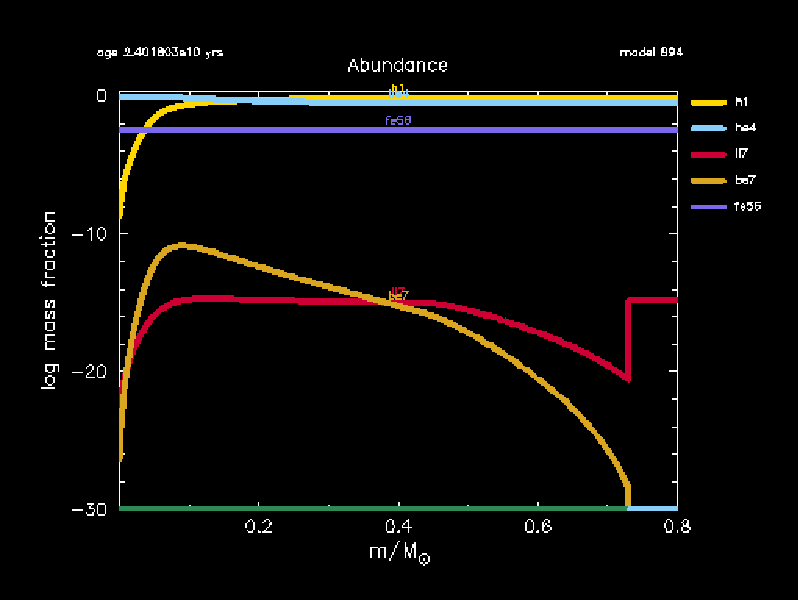
\includegraphics[width=0.5\textwidth]{img/tesis/abundances.pdf}
    \caption {Gráfica de abundancias en la que aparecen los elementos H, He, Fe, Li y Be. El eje de abscisas ha sido reescalado}
    \label{fig:abundances}
\end{figure}

Continuando con el marco físico a simular, pasamos a centrarnos en la activación de los mecanismos que, acorde a la teoría, tienen influencia en el agotamiento del Li:
\begin{itemize}
    \item Proceso de difusión
    \item Proceso de rotación
\end{itemize}

Como ya se indicaba en el apartado \ref{subsec_diffusion}:
\begin{center}
    \begin{minipage}{0.9\linewidth}
        \vspace{5pt}%margen superior de minipage
        {\small
        (MESA) calcula la difusión de partículas y la sedimentación gravitacional resolviendo las ecuaciones de Burger a través del método propuesto por Thoul \cite{Thoul1993}. El módulo de difusión trata los elementos presentes en el modelo estelar como pertenecientes a "clases" definidas por el usuario en términos de rangos de masas atómicas.
        }
        \vspace{5pt}%margen inferior de la minipage
    \end{minipage}
\end{center}

De esta información se desprende que el hecho de que al activar la difusión también activamos la sedimentación gravitacional y, de manera indirecta, el módulo \textit{mlt} encargado de calcular los coeficientes de difusión que entran en juego en proceso de mezclado producido a consecuencia de los movimientos convectivos que se produce en el interior de la estrella.\par

Cabe también mencionar el tratamiento por “clases” que realiza MESA. Los isótopos presentes en nuestra red de reacciones nucleares que tienen un peso atómico similar son tratados de forma conjunta por la rutina de difusión en lo que se refiere a su velocidad de difusión. Ésta queda determinada por el isótopo representativo de la “clase”. La agrupación en clases tiene la ventaja de que las simulaciones se ejecutan de una manera más rápida ya que se ahorran cálculos. Por otra parte, tiene el inconveniente de que los resultados pueden llegar a ser menos exactos. En este trabajo hemos optado por desactivar la agrupación en clases a costa de aumentar los tiempos de simulación.\par

En lo que se refiere a la rotación de las capas superficiales de la estrella, MESA permite especificar una velocidad en km/s, que en nuestro caso ha quedado fijada en 20 km/s al ser un valor similar al que tenemos en el Sol.\par

En el Listado \ref{lst:net_params} mostramos la configuración adicional a añadir al proyecto de MESA para poder simular los conceptos teóricos discutidos hasta este momento.
\begin{lstlisting}[language=Fortran, caption={Parametrización de los procesos relacionados con el Li y de las gráficas de salida.}, label={lst:net_params}]
&star_job
  ! Change default net in order to include 
  !reactions for Li and Be
  change_initial_net = .true.
  new_net_name = 'pp_extras.net'
  ! If enable_adaptive_network is true, 
  ! then at each step, 
  ! the system calculates a new set of isos. 
  ! This can cause significant slowdowns
  enable_adaptive_network = .true.

  ! Activate surface rotation and set velocity
  change_v_flag = .true.
  new_v_flag = .true.
  set_initial_surface_rotation_v = .true.
  new_surface_rotation_v = 20 ! km/sec 

  ! Rotation off until near ZAMS
  change_rotation_flag = .false.
  new_rotation_flag = .true.

&controls
  ! toggle element diffusion
  do_element_diffusion = .true.
  ! If true, don't lump elements into 
  ! classes for diffusion. 
  ! Instead, each isotope in the network 
  ! is treated as its 
  ! own separate class. This can cause 
  ! significant slowdowns 
  ! for large nets, so it is off by default.
  diffusion_use_full_net = .true.
  diffusion_use_cgs_solver = .false.

&pgstar
  ! show HR diagram
  ! this plots the history of L,Teff 
  ! over many timesteps
  HR_win_flag = .true.

  ! configure file output 
  HR_file_flag = .true.
  HR_file_interval = 1


  ! show the abundance profile
  Abundance_win_flag = .true.
  num_abundance_line_labels = 1

  ! set how many elements must be shown
  Abundance_num_isos_to_show = 5
  Abundance_which_isos_to_show(1) = 'li7'
  Abundance_which_isos_to_show(2) = 'be7'
  Abundance_which_isos_to_show(3) = 'h1'
  Abundance_which_isos_to_show(4) = 'he4'
  Abundance_which_isos_to_show(5) = 'fe56'

  ! set the max and min value for the y-axis
  Abundance_log_mass_frac_min = -30
\end{lstlisting}

Llegado este punto, hemos conseguido obtener una configuración de proyecto base que recoge las características esenciales de la estrella a simular en MESA, pone en marcha los procesos físicos relacionados con la evolución del Li y es capaz de informar, tanto a través de los ficheros de salida estándar como de las representaciones gráficas, sobre las abundancias de Li a lo largo de la evolución de la estrella en sus etapas de PMS y MS. Como decimos, esta configuración de proyecto y los valores arrojados por la simulación que lo utiliza, nos servirán para establecer el marco de referencia contra el que comparar los valores obtenidos en las nuevas simulaciones que extienden la funcionalidad de MESA.\par

--CONTINUAR POR AQUÍ --

\subsection{Simulaciones extendiendo el marco teórico estándar de MESA}
Una vez que hemos llegado a un punto en el que tenemos una configuración de proyecto que nos permite obtener las abundancias de Li de forma detallada, y además hemos conseguido activar los procesos de difusión y rotación superficial en nuestro modelo, damos paso a una segunda línea de trabajo consistente en extender el funcionamiento de MESA para incorporar nuestras propias rutinas de extensión al simulador. Las consideraciones previas a tener en cuenta son las siguientes:

--INCLUIR AQUÍ ENUMERACIÓN DE PASOS A GRANDES RASGOS--
\begin{itemize}
    \item Entender el ciclo de control aplicado a los pasos de simulación
    \item Extender la rutina de inicialización para incorporar nuestros parámetros
    \item Extender 
\end{itemize}

El planteamiento teórico no es especialmente difícil, lo complicado del mismo es la parte que afecta a MESA. En concreto, localizar las secciones concretas de código en las que se calcula el valor de la gravedad local que afecta a cada elemento de masa que tiene en cuenta la simulación. A esto hay que sumarle el hecho de que MESA está construido de una forma modular, así que es de esperar que no tengamos una única sección de código en el programa donde se calcule este valor de gravedad, sino que cada módulo que, de algún u otro modo, contribuya a la difusión química de los elementos tiene que ser revisado.\par

Con diferencia, el localizar dónde invocar a nuestra rutina de código es la parte más complicada de todo el presente trabajo. Tenemos que detectar los módulos implicados en la difusión de los elementos, con el riesgo que implica que nos dejemos alguno por identificar, analizar su código fuente en detalle para llegar a entender su funcionamiento y realizar la invocación en el punto exacto a nuestra rutina, para alterar así el valor de gravedad calculado por MESA para un determinado diferencial de masa. Adicionalmente, se hace totalmente necesario el revisar la bibliografía en la que se basa la implementación de las rutinas presentes en cada módulo para dotar de contexto y significado a las líneas de código. De otro modo, es casi imposible extraer el trasfondo científico que se encuentra en ellas codificado.\par

--REVISAR PARA ELIMINAR REFERENCIAS A GRAVEDAD. HACERLO GENÉRICO--

Inicialmente teníamos dos módulos candidatos por los que empezar a estudiar su implementación, el de difusión y el de mlt. Por tener éste último un menor número de líneas de código (aproximadamente unas 1800) y encontrarse la implementación restringida a un solo módulo, empezamos por él. Tras una revisión a fondo del mismo se llegó a generar una versión modificada del mismo que calculaba un nuevo valor de gravedad local relacionado con el elemento de masa diferencial. Este nuevo valor tenía en cuenta tanto la masa del planeta, como su distancia a la estrella.\par

Seguidamente pasamos a analizar el código fuente del módulo de difusión que, como mencionábamos, se basa en la implementación de las ecuaciones propuestas en el trabajo de Thoul, et al. (1994). Ya desde los primeros momentos nos dimos cuenta de que el esfuerzo de localizar dónde deberíamos de invocar a nuestra rutina se iba a complicar. La implementación de este módulo es bastante más laboriosa, larga (más de 3500 líneas) y se encuentra repartida entre varios módulos que, a diferencia de lo que ocurría con el de mlt, algunos de ellos no ofrecían la posibilidad de ser extendidos de una manera cómoda. Además de esto, la implementación que se sigue en MESA acaba generando una matriz de coeficientes de difusión en los que el efecto de la gravedad está representado de manera implícita, es decir, no se calcula un valor de gravedad local asociada a un elemento diferencial de masa en un paso previo, de forma análoga a como ocurre en el módulo de mlt, para finalmente acabar derivando el valor del coeficiente de difusión. En este caso se resuelve el sistema de ecuaciones y la contribución de la gravedad sobre el elemento de masa queda recogida en las soluciones al mismo. A la propia dificultad de entender la implementación del código, se sumaba el hecho de tener que deshacer el cálculo de los coeficientes para poder incluir el efecto de nuestra rutina, y esto era algo que se antojaba harto complicado al no disponerse del conocimiento necesario. Estábamos en un punto muerto.

--REVISAR PARA ELIMINAR REFERENCIAS A GRAVEDAD--

\subsection{Rutina de inicialización para las simulaciones}
EXPLICAR EL CONJUNTO DE PARÁMETROS QUE SE LEEN DEL INLIST, Y SIGNIFICADO. TAMBIÉN LOS FLAGS DE DEPURACIÓN
\begin{lstlisting}[language=Fortran, caption={Rutina de inicialización de las simulacions.}, label={lst:extras_ctrl}]
      subroutine extras_controls(id, ierr)
         integer, intent(in) :: id
         integer, intent(out) :: ierr
         type (star_info), pointer :: s
         ierr = 0
         call star_ptr(id, s, ierr)
         if (ierr /= 0) return
         
         original_diffusion_dt_limit = s% diffusion_dt_limit
         s% other_wind => Reimers_then_Blocker
         ! inject our torque routine
         s% other_torque => other_torque_hook

         !debug flags
         debug_use_other_torque = s% x_logical_ctrl(1)
         debug_reset_other_torque = s% x_logical_ctrl(2)
         debug_get_cz_info = s% x_logical_ctrl(3)
         debug_get_core_info = s% x_logical_ctrl(4)
         debug_new_alpha = s% x_logical_ctrl(7)
         debug_mag_field = s% x_logical_ctrl(8)
         debug_j_dot = s% x_logical_ctrl(9)

         !If true, once the radiative core is developed, report always true
         !in is_radiative_core function
         keep_on_rad_core = s% x_logical_ctrl(6)

         !eps thershold
         eps_threshold = s% x_ctrl(2)

         !disk locking
         disk_lt = s% x_ctrl(3)
         disk_omega = s% x_ctrl(4)

         !Variable MLT alpha
         var_mlt_alpha = s% x_logical_ctrl(10)
      
         ! Once you have set the function pointers you want,
         ! then uncomment this (or set it in your star_job inlist)
         ! to disable the printed warning message,
         ! Uncomment these lines if you wish to use the functions in this file,
         ! otherwise we use a null_ version which does nothing.
         s% extras_startup => extras_startup
         s% extras_start_step => extras_start_step
         s% extras_check_model => extras_check_model         
         s% extras_finish_step => extras_finish_step
         s% extras_after_evolve => extras_after_evolve
         s% how_many_extra_history_columns => how_many_extra_history_columns
         s% data_for_extra_history_columns => data_for_extra_history_columns
         s% how_many_extra_profile_columns => how_many_extra_profile_columns
         s% data_for_extra_profile_columns => data_for_extra_profile_columns  
         
         s% job% warn_run_star_extras =.false.             
      end subroutine extras_controls
\end{lstlisting}

\subsection{Rutina de par de torsión}
EXPLICAR QUE SUSTITUIMOS LA RUTINA POR DEFECTO CON LA NUESTRA
\begin{lstlisting}[language=Fortran, caption={Rutina de par de torsión.}, label={lst:torque_hook}]
      subroutine other_torque_hook(id, ierr)
         use const_def
         integer, intent(in) :: id
         integer, intent(out) :: ierr
         type (star_info), pointer :: s

         ierr = 0
         call star_ptr(id, s, ierr)
         if (ierr /= 0) return


         !If disk locking is actived & the star is younger that disk 
         !locking period &
         !star rotates faster than disk locking rotational velocitiy
         if((disk_lt>0).and.(s%star_age<disk_lt).and.(s%omega(1)>disk_omega)) then
            call other_torque_disk_lock(id, ierr)
         else
            call other_torque_mag_brk(id, ierr)
         endif
         
      end subroutine other_torque_hook
\end{lstlisting}

\subsection{Rutina de frenado magnético}
EXPLICAR QUE LOS DOS TIPOS DE RUTINAS: INTESIDAD FIJA, INTENSIDAD VARIABLE
\begin{lstlisting}[language=Fortran, caption={Rutina de frenado magnético.}, label={lst:torque_mb_hook}]
      ! This routine implements a magnetic braking effect.
      ! It distributes among the zones which conforms the convective shell the
      ! loss of angular momentum
      subroutine other_torque_mag_brk(id, ierr)
         use const_def
         integer, intent(in) :: id
         integer, intent(out) :: ierr
         type (star_info), pointer :: s
         integer :: k
         real(dp) :: B, j_dot, r_st
         type (star_zone_info), target :: sz_info, core_info
         type (star_zone_info), pointer :: sz_info_ptr, core_info_ptr
         real(dp), dimension(:), pointer :: mag_brk_jdot
         integer :: jdot_routine !how to distribute the j_dot
         !controls if jdot distribution must only affect the convective zone
         logical :: only_cz
         !controls if jdot distribution must wait till a radiative core is develop
         logical :: wait_rad_core          
         integer :: activated !signals when the jdot routine is activated
         
         !Pointer to structure which conveys information about the convectice
         !and core zones
         sz_info_ptr => sz_info
         core_info_ptr => core_info

         ierr = 0
         call star_ptr(id, s, ierr)
         if (ierr /= 0) return


         !Reset support structures
         allocate(mag_brk_jdot(s% nz))
         s% extra_jdot(:) = 0
         s% extra_omegadot(:) = 0
         activated = 0
         call reset_x_ctrl(s, idx_low_x_ctrl, idx_high_x_ctrl)
         call reset_core_info(core_info_ptr)
         call reset_convective_info(sz_info_ptr)

         !Wait till radiative core is develop?
         wait_rad_core = s% x_logical_ctrl(5)

         !Loss of angular momentum distribution method
         jdot_routine = s% x_integer_ctrl(1)
         only_cz = .true.
         if (jdot_routine /= 0) then
               only_cz = .false.
         end if

         !Get information about the convective zone
         if (only_cz) then
            !Get information about the outter convective zone
            call get_convective_info(s, sz_info_ptr)
         else
            !Get information about the outter convective zone till star surface
            call get_convective_to_surf_info(s, sz_info_ptr)
         end if

         !Get information about the core
         call get_core_info(s, core_info_ptr)


         !Calculate amount of loss of angular moment
         !Magentic field intensity
         B = s% x_ctrl(1)
         if (B < 0) then
            B = calculate_mag_field_intensity_gb(s)
            j_dot = calculate_jdot_rate_gb(s, B)
         else
            j_dot = calculate_jdot_rate_cantiello(s, B)
         end if
         

         ! The MB routine is activated under the following conditions:
         ! - use_other_torque flag is activated in inlist
         ! AND
         ! - the star is losing mass
         ! AND
         ! - the magnetic field intensitive is bigger than 0.0 (allow to 
         ! execute the routine if use_other_torque=.true.)
         ! AND
         ! (
         !   - a radiative core developed isn't required (configured in inlist)
         !   OR
         !   - a radiative core is required AND this was developed
         !)
         if ((s% use_other_torque) .and. (s% mstar_dot<0.0) .and. (B>0.0) .and. &
            (.not. wait_rad_core .or. (wait_rad_core .and. is_core_rad(s)))) then

            activated = 1

            !Distribute the loss of angular momentum
            call distribute_j_dot(s, j_dot, sz_info_ptr, mag_brk_jdot)

            !It happens that s% extra_jdot is longer than s% nz but mag_brk_jdot
            !is just defined
            !for s% nz elements
            s% extra_jdot(1:s% nz) = mag_brk_jdot
         end if
      end subroutine other_torque_mag_brk
\end{lstlisting}

\endinput
%--------------------------------------------------------------------
% FIN DEL CAPÍTULO. 
%--------------------------------------------------------------------


% !TeX root = ../libro.tex
% !TeX encoding = utf8


\chapter{Resultados de frenado magnético de intensidad fija}\label{ch:quinto-capitulo}
\section{Configuración de los modelos} \label{marco_teorico}
A COMENTAR
Parametrización de los modelos
Rango de valores a asignar a los parámetros libres
Ciclo de control
Para cada paso de simulación
- Obtenemos o calculamos la intensidad del campo magnético
- Calculamos la pérdida de momento angular inducida por el campo magnético
- Distribuimos la pérdida de momento angular entre las capas de la estrella
- Obtenemos o calculamos el valor de $\amlt$


\section{Modelos de evolución estelar}
De acuerdo con la formulación de las secciones anteriores, los dos únicos parámetros libres de nuestra implementación son $B$ y $\Omega$. Las simulaciones numéricas trazaron la historia rotacional y $A(\isotope[7]{Li})$ de una estrella 1 $\msun$ para una variedad de valores iniciales para $B$ y $\Omega$ (ver también Tabla \ref{tab:phy_mesa}). MESA utiliza el enfoque en capas (shellular) \cite{Meynet1997} para dar cuenta de los efectos hidrostáticos de la rotación en modelos estelares 1D.\par

\begin{table}
	\begin{threeparttable}
		\centering
		\begin{tabular}{ll} 
			\hline
			Parámetro & Prescripciones y valores adoptados\\
			\hline
			Abundancia Solar & $X_{\odot}=0.7154, Y_{\odot}=0.2703, Z_{\odot}=0.0142$\\
			Ecuación de estado & OPAL+SCVH+MacDonald+HELM+PC\\
			Opacidad & OPAL Tipo I para log T $\geq$ 4 \\ & Ferguson para logT $<$ 4\\
			Tasas de Reacción & JINA REACLIB\\
			Condiciones de Contorno & ATLAS12; $\tau$=100 tablas + fotoesfera\\
			Difusión & Rastreo de \isotope[1]{H}, \isotope[2]{He}, \isotope[7]{Li}, \isotope[7]{Be}\\
			Esquema de Rotación & Rotación diferencial en PMS \& MS\\ & Incluye SH\tnote{1}  , ES\tnote{2}  , GSF\tnote{3}  , SSI\tnote{4}  , DSI\tnote{5}\\
			Termohalina & $\alpha_{\textrm{th}}=666$\\
			Convección & $\alpha_{MLT}$ = 1.82 + Ledoux\\
			Semiconvección & $\alpha_{sc}=0.1$\\
			Sobreimpulso & $f_{ov,core}=0.0160$, \& $f_{ov,sh}=0.0174$\\
			Campo Magnético & B(G) prefijado con valores puntuales entre [3.0 - 5.0]\\
			Pérdida de Masa & $\Dot{M}_{\textrm{max}} = 10^{-3} \: \msun \: yr^{-1}$\\
			Périda de Momento Angular & $\Dot{J} = \frac{2}{3} \mwind \;\Omega_*\; \ralfven^2$\\
			\hline
		\end{tabular}
		\begin{tablenotes}\footnotesize
			\item (1) Solberg-Hoiland, (2) Eddington–Sweet
			\item (3) Goldreich–Schubert–Fricke, (4) Secular Shear Instability
			\item (5) Dynamical Shear Instability
		\end{tablenotes}
	\end{threeparttable}
	\caption{Resumen de la física adoptada en MESA \cite{Choi2016}[basado en][].}
	\label{tab:phy_mesa}
\end{table}



Adoptamos abundancias a escala solar y asumimos una abundancia inicial solar ($Z = Z_{\odot, \mathrm{pr} = 0.0142}$). También adoptamos los siguientes valores nominales para expresar las propiedades estelares en unidades SI, $\rsun = 6.957x10^{10}\, cm$ y $\msun = 1.988x10^{33}\, g$ que son coherentes con las resoluciones de la IAU \cite{Mamajek2015}. Para una descripción detallada de la física adoptada en este trabajo, remitimos al lector a \cite{Choi2016}. Ese trabajo se utilizó como punto de partida para el nuestro en lo que respecta a la parametrización del proyecto MESA, que se calibró para reproducir las abundancias de elementos medidas en la superficie solar.\par

Los modelos incluyeron la rotación durante la PMS ya que existen evidencias que abogan por una fuerte relación establecida entre la destrucción de Li y la rotación en esa fase (\cite{Bouvier2016,Bouvier2018}). Modelamos la rotación como AML se calcula como resultado del par aplicado a la zona de convección por un viento acoplado magnéticamente. Además, no tuvimos en cuenta ni la influencia de los campos magnéticos internos ni su existencia durante la fase T-Tauri.\par 
---CORREGIR ESTO SEGUN EL NUEVO PAPERAdoptamos un enfoque teórico sencillo y pragmático para establecer cuándo la estrella está alcanzando la fase ZAMS. El criterio elegido se basó en la existencia simultánea de una extensa capa convectiva y un núcleo radiativo. A partir de este momento, se activó la rutina MB, actuando como un mecanismo adicional a los existentes en el código evolutivo MESA que participó en el AML de la estrella. ---HASTA AQUÍ---\par

Supusimos que el campo magnético no variaba su intensidad a lo largo de la evolución de la estrella hasta alcanzar el TAMS. Además, también se consideraron otros efectos de rotación durante la evolución de los modelos: el transporte de AM desde el interior radiativo hasta la envoltura convectiva y la redistribución de AM asociada a cambios en la estructura interna durante el proceso de contracción hacia la EM.\par

Nos centramos en el papel indirecto que desempeña el MB en la destrucción del Li. Esto es consecuencia de su influencia en la historia rotacional de las estrellas de tipo solar. Nuestro principal objetivo era comprobar cómo el MB podría contribuir a explicar la evolución del Li en el Sol y en otras estrellas de tipo solar. Se ejercitaron un conjunto de escenarios diferentes con intensidades de campo magnético que oscilaban entre 3,0 y 5,0 G. Calculamos la evolución de modelos estelares 1 $\msun$ con metalicidad inicial solar y $\oomegac$ variable entre $0.0084$ y $0.0336$. Hemos adoptado el siguiente enfoque teórico para establecer cuándo la estrella está alcanzando la ZAMS: cuando tanto la fracción de masa central del \isotope[1]{H} se ha reducido en $\Delta( \isotope[1]{H})= 0.0001$ respecto a su valor inicial, como la luminosidad de la estrella ($L$) está casi totalmente ($L \geq 0.99$) generada por las reacciones nucleares del \isotope[1]{H} ocurren simultáneamente. \par

Como expresa la Ec.~\ref{eq:j_dot_mesa}, la cantidad de AML depende de $R_A$ (o alternativamente de $\eta_*$), $\Omega$ y $\Dot{M}$. Para un valor grande de $\eta_*$, la estrella experimenta una desaceleración significativa. Controlamos el valor de $\eta_*$ en los modelos variando el campo magnético ($B$) y la velocidad de rotación estelar ($\Omega$). Con respecto a $\Dot{M}$ y como se indica en la tabla \ref{tab:phy_mesa}, para calcular la pérdida de masa se utilizó la fórmula empírica desarrollada por Reimers \cite{Reimers1975} para estrellas en la rama gigante asintótica (AGB). Para una estrella de tipo solar el $\Dot{M}$ durante la EM es relativamente pequeño, alrededor de $10^{-14}\msun \, yr^{-1}$ \cite{Noerdlinger2008}. \par

\subsection{Evolución de Li sin MB}

\begin{figure}
    \centering
	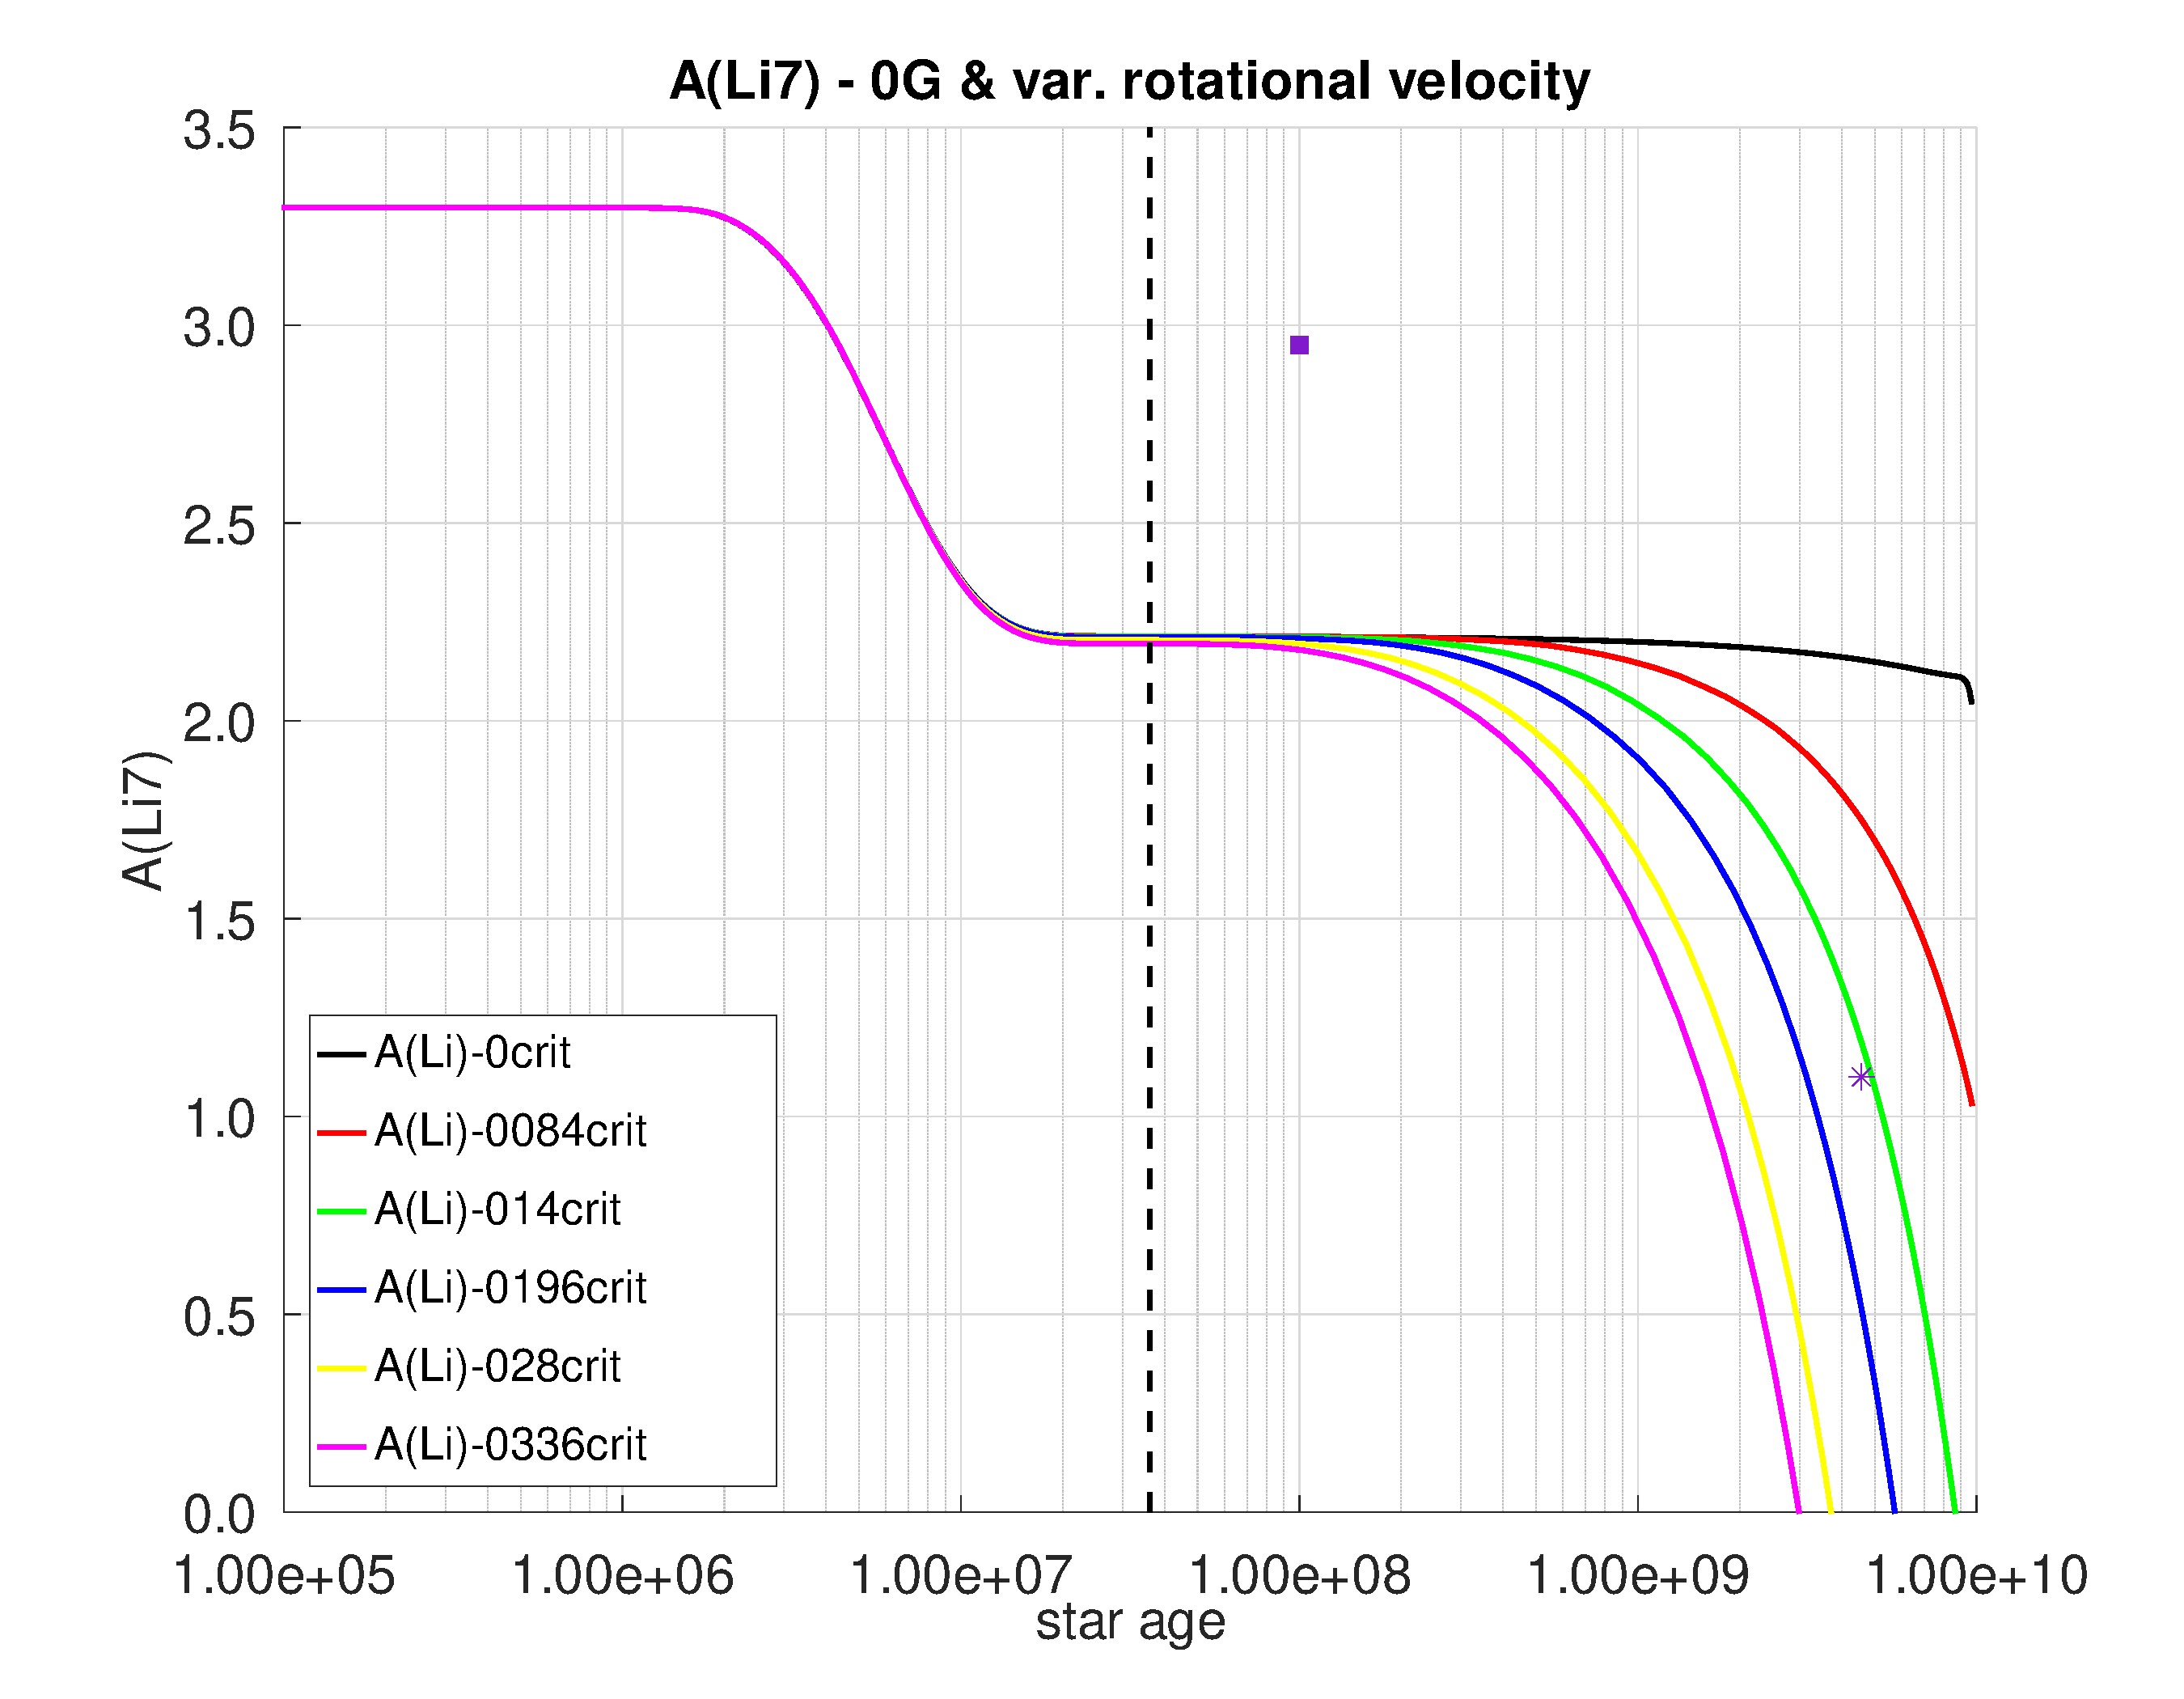
\includegraphics[width=0.7\textwidth]{img/paper1/li_var_vel_0_0g.pdf}
	\caption{La evolución de la abundancia superficial del \isotope[7]{Li} en relación con el \isotope[1]{H}, en función del tiempo para varios modelos de 1 $\msun$. La línea negra continua representa el modelo de referencia según \cite{Choi2016}. El resto de líneas son modelos que incluyen rotación PMS con $\oomegac$ entre 0.0084 y 0.0336, respectivamente. La estrella púrpura y el cuadrado son abundancias superficiales de Li para el Sol actual \cite{Asplund2009} y la media para el cúmulo de las Pléyades \cite{Sestito2005} respectivamente. La línea vertical discontinua hace referencia a la ZAMS.}
	\label{fig:li_var_vel_0g}
\end{figure}

La figura \ref{fig:li_var_vel_0g} muestra la evolución temporal de la abundancia superficial de Li para varios modelos $1\msun$ inicializados con diferentes velocidades de rotación. Las simulaciones tuvieron en cuenta los efectos de rotación y AML causados por los vientos estelares pero no los de MB. La estrella púrpura y el cuadrado son las abundancias superficiales de Li para el Sol actual \cite{Asplund2009} y para las Pléyades, respectivamente \cite{Sestito2005}.\par

Obsérvese cómo la abundancia de Li en la superficie estelar disminuyó con el tiempo para todos los modelos simulados. La línea negra continua representa el modelo de referencia que adopta los parámetros de superación de la envoltura calibrados para el Sol, como se documenta en \cite{Choi2016}. Todos los modelos quemaron demasiado Li antes de la ZAMS y, por tanto, no coincidieron con la abundancia media de Li en superficie de las Pléyades. También fue destacable el hecho de que apenas hubo diferencias entre los distintos modelos en cuanto a la abundancia de Li durante gran parte de la ZAMS. Sólo después de un millón de años se destruyó el Li en un grado acentuado, ya que antes no se alcanzó la temperatura necesaria en BCZ. Después, los diferentes modelos destruyeron el Li de forma muy similar debido a dos razones principales. Por un lado, las zonas convectivas que desarrollaron los modelos tenían tamaños muy similares, por lo que la temperatura en la BCZ era prácticamente la misma. Por otro lado, el diferencial de rotación entre el núcleo y la zona convectiva no comenzó a desarrollarse hasta que alcanzó los $ \approx 10^6$ años, alcanzando su máxima diferencia en la ZAMS alrededor de los $ \approx 10^7$ años. Fue en este momento cuando debieron aumentar los efectos combinados de la turbulencia y la diferencia rotacional, dando lugar a notables diferencias en la evolución de A(Li) (véase la figura \ref{fig:li_var_vel_0g_z1}). Posteriormente, el modelo de referencia (línea negra) no agotó eficientemente el Li en la EM y no consiguió (de nuevo) igualar la abundancia actual de Li en la superficie solar. Los otros modelos que incluían la rotación durante el PMS con valores de $\oomegac$ entre 0.0084 y 0.0336 fueron capaces de quemar Li de forma más realista. Entre ellos, sólo uno (línea verde) se aproximaba a la abundancia actual de Li del Sol, pero su velocidad de rotación era mucho mayor (véase la figura \ref{fig:rot_vel_0g}) que los $2\,\kms$ del Sol \cite{Gill2012}. \par

Durante gran parte del PMS la estrella giró como un cuerpo sólido (véase la Figura \ref{fig:rot_vel_0g}) y esto se debió a que la estrella tenía un interior totalmente convectivo. No fue hasta el final de la trayectoria de Hayashi cuando la estrella comenzó a desarrollar un núcleo radiativo. Fue en esta etapa cuando apareció una diferencia de velocidad angular entre los límites superior e inferior de las zonas radiativa y convectiva respectivamente. El grado de rotación diferencial estaba directamente influido por la $\Omega$ inicial. A medida que los modelos se inicializaban con una velocidad angular mayor, se acentuaba la diferencia de velocidad entre la BCZ y la superficie estelar; cuanto mayor era la velocidad inicial, mayor era el gradiente de velocidad entre los límites inferior y superior de la CZ. Como consecuencia, la fuerza de la turbulencia localizada en la BCZ aumentó, de modo que el Li pudo alcanzar regiones con temperaturas cercanas a $\tli$, donde finalmente se quemó y destruyó (véase la figura \ref{fig:li_var_vel_0g}). Otras investigaciones \cite{Bouvier2018, Baraffe2017} apuntan a una tendencia diametralmente opuesta a la aquí expuesta, es decir, a mayor velocidad de rotación, mayor abundancia de Li en la superficie de la estrella. \par

\begin{figure}
    \centering
    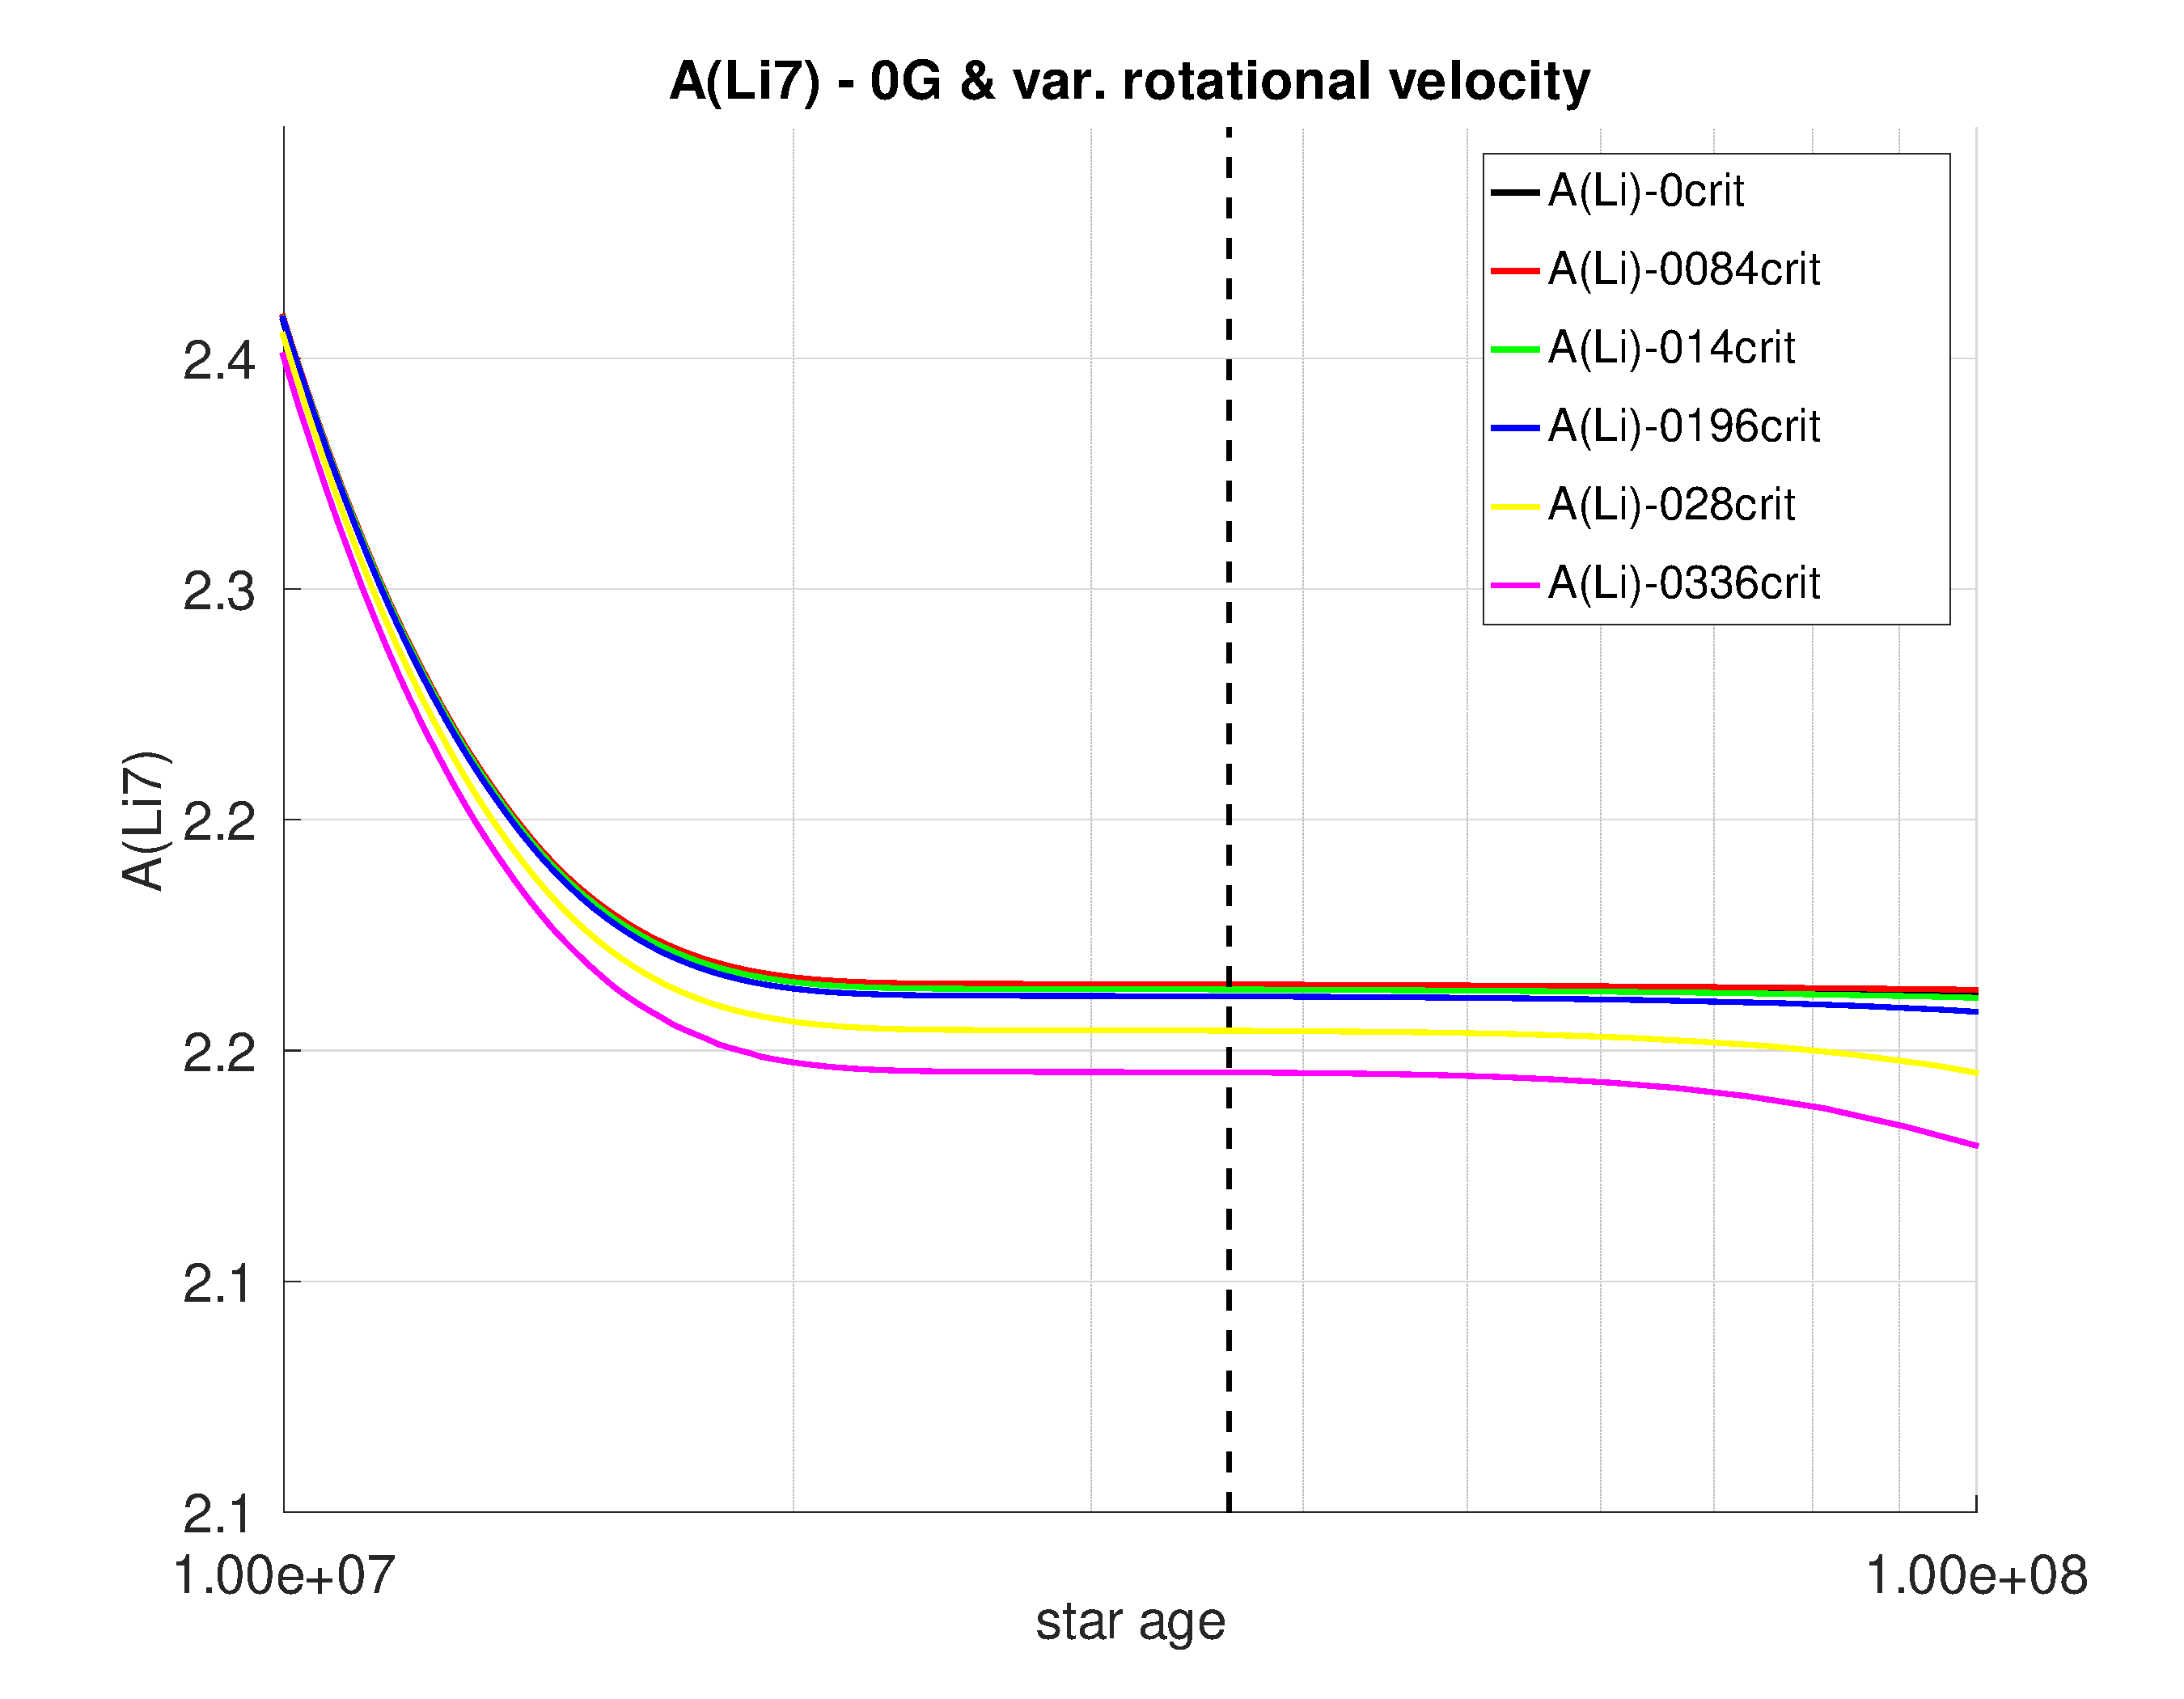
\includegraphics[width=0.7\textwidth]{img/paper1/li_var_vel_0_0g_z1.pdf}
	\caption {Similar a la Figura \ref{fig:li_var_vel_0g} pero ampliando la ZAMS. Los modelos con una mayor velocidad de rotación inicial alcanzan ya la ZAMS con una menor cantidad de medida de Li en la superficie estelar.}
	\label{fig:li_var_vel_0g_z1}
\end{figure}

\begin{figure}
	\centering
	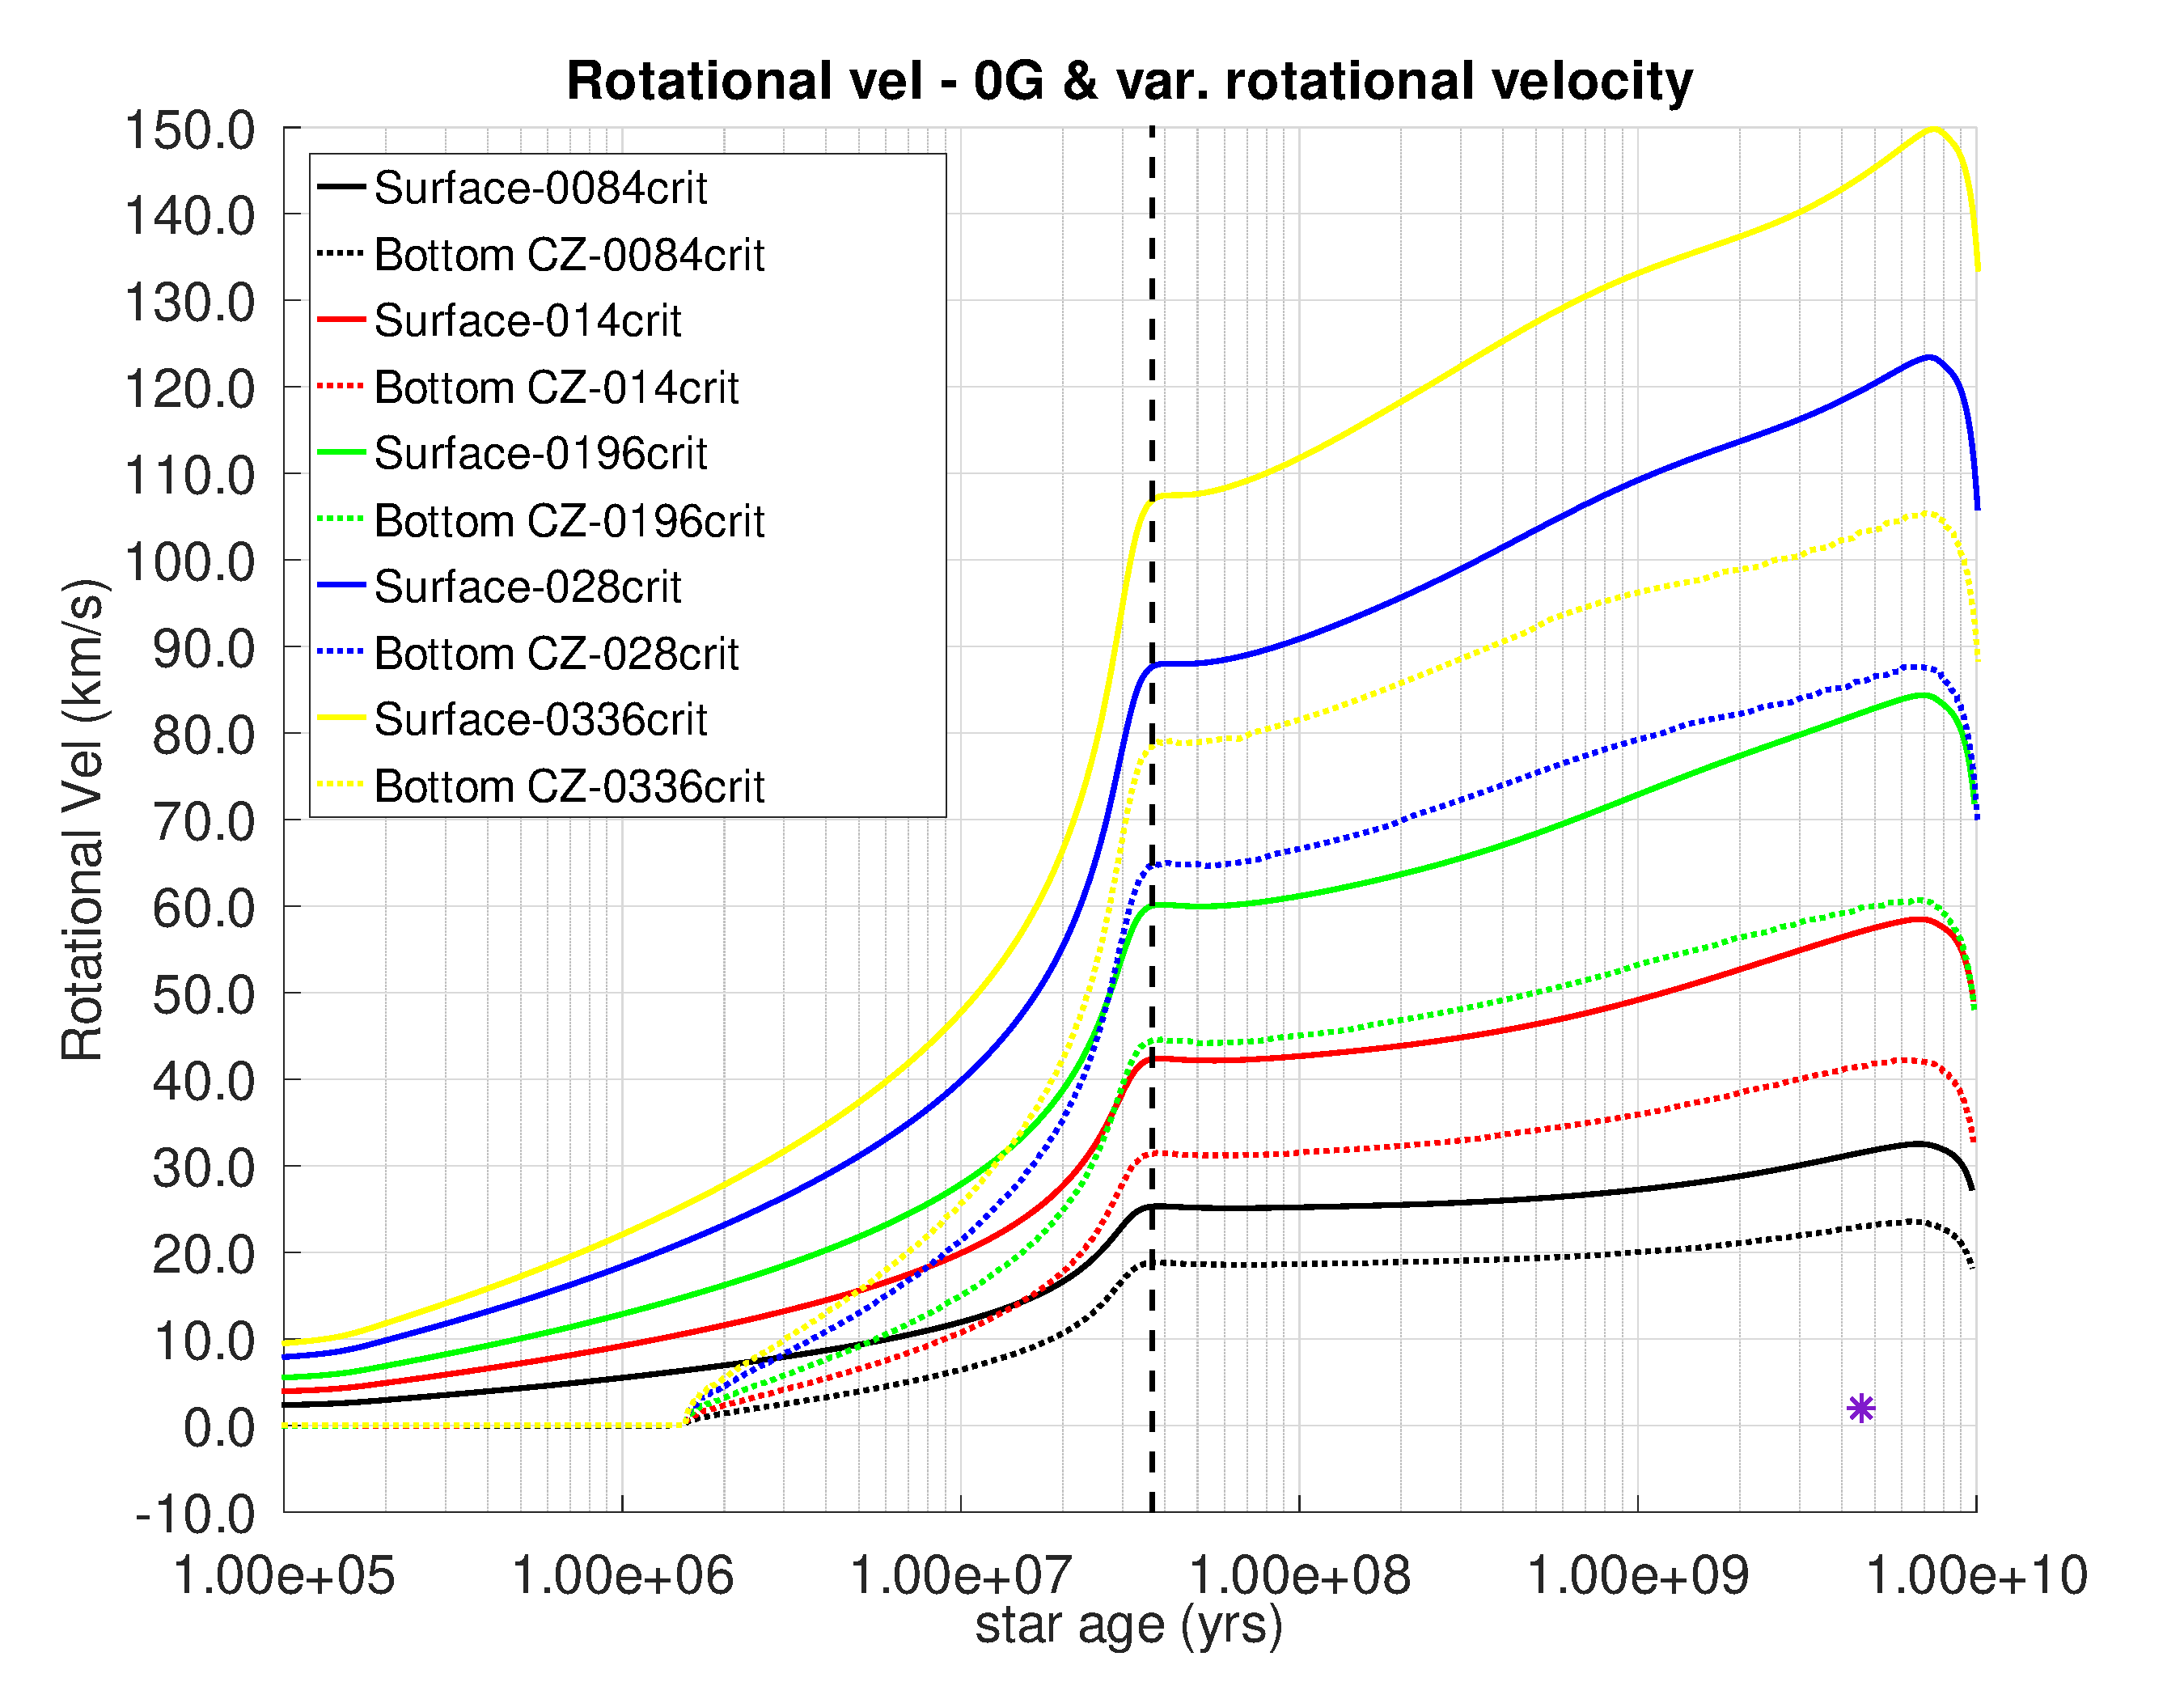
\includegraphics[width=0.7\textwidth]{img/paper1/rot_vel_var_vel_0_0g.pdf}
	\caption{Evolución de la velocidad angular en la superficie (línea continua) y en el límite inferior (línea discontinua) de la zona convectiva superior, en función del tiempo para varios modelos de 1 $\msun$. Los modelos incluyen rotación PMS con valores $\oomegac$ entre 0,0084 y 0,0336. La estrella púrpura es la velocidad angular superficial para el Sol actual \cite{Gill2012}. La línea vertical discontinua hace referencia a la ZAMS.}
	\label{fig:rot_vel_0g}
\end{figure}

Otros efectos estructurales bien conocidos de la rotación son la disminución de la temperatura efectiva ($\teff$) y, en menor medida, de la luminosidad estelar ($L$). Ambos efectos pueden observarse gráficamente en el diagrama HR de la figura \ref{fig:hr_var_vel_0g}, que muestra una vista ampliada de las trayectorias evolutivas desde la ZAMS hasta la TAMS para varios modelos $\msun$ inicializados con diferentes velocidades de rotación. Si comparamos el modelo no rotatorio (línea sólida negra) con los rotatorios podemos reconocer que al final del PMS, estos últimos alcanzan la ZAMS con un $\teff$ menor que los primeros. Estos resultados coinciden con los de estudios anteriores \cite[véase por ejemplo ][]{Eggenberger2012,Piau2001,Pinsonneault1989}.\par

\begin{figure}
    \centering
    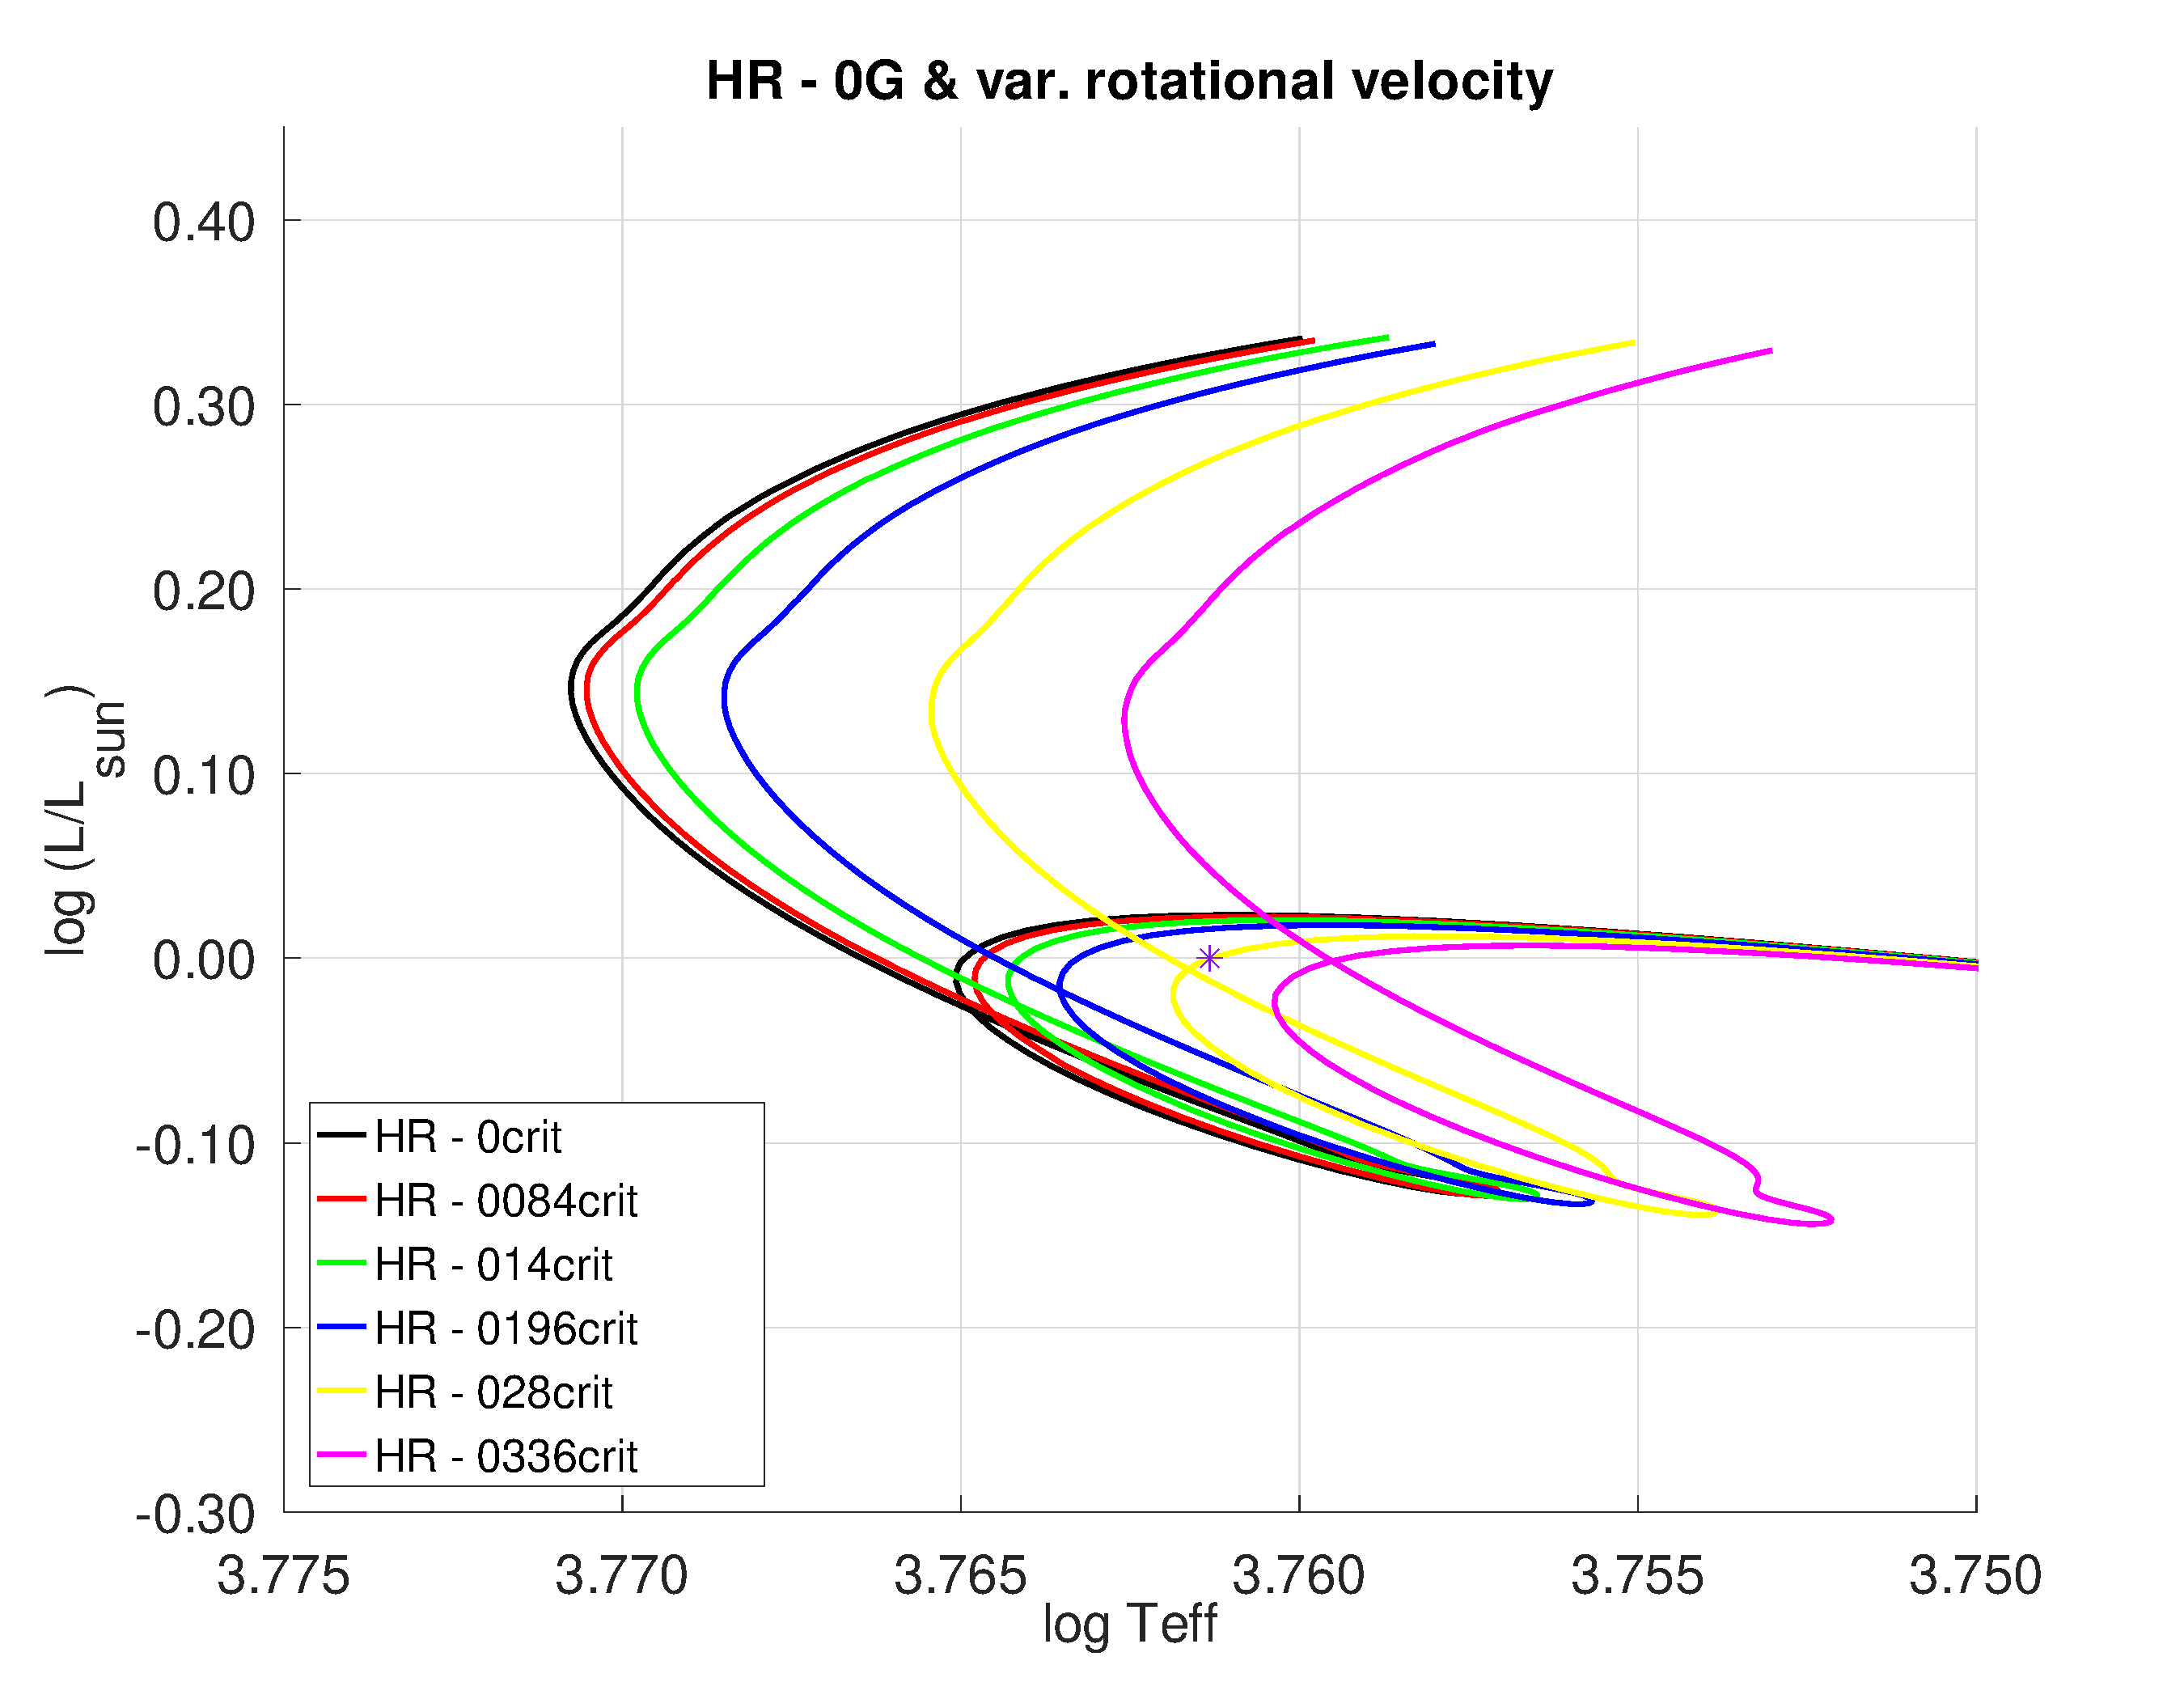
\includegraphics[width=0.7\textwidth]{img/paper1/hr_var_vel_0_0g_z1.pdf}
	\caption{Un ejemplo de cuadrícula solar de 1$\msun$ de trayectoria evolutiva estelar desde el PMS hasta el TAMS cubriendo un amplio rango de velocidades angulares. La rotación se activa en los modelos en el PMS y esos modelos llegan antes a la ZAMS y a un $\teff$ menor que el de no rotación (línea negra continua). La luminosidad se expresa en términos de $\lsun$.}
	\label{fig:hr_var_vel_0g}
\end{figure}

\subsection{Evolución del Li con MB de intensidad fija}
La figura \ref{fig:li_var_vel_4_0g} muestra la evolución temporal de la abundancia superficial de Li para varios modelos de 1 $\msun$. Estos modelos se inicializaron con diferentes velocidades rotacionales y tuvieron en cuenta los efectos del MB causado por un campo magnético de intensidad 4G. Si lo comparamos con la Figura \ref{fig:li_var_vel_0g} en la que se despreciaron los efectos del MB, observamos cómo se alteraron los perfiles de abundancia de Li durante el PMS y el MS. Durante el PMS podemos describir el efecto como modesto, algo esperado y en línea con el hecho de que el AML causado por MB (ver Ec.~\ref{eq:j_dot}) depende directamente de la tasa de pérdida de masa. Si tenemos en cuenta que para las estrellas de tipo solar los modelos predicen una tasa de pérdida de masa total modesta, ese valor es incluso mucho menor en esta fase. Por el contrario, durante la EM se observa que la AML es mucho más significativa, provocando que se destruya una menor cantidad de Li.\par

\begin{figure}
    \centering
    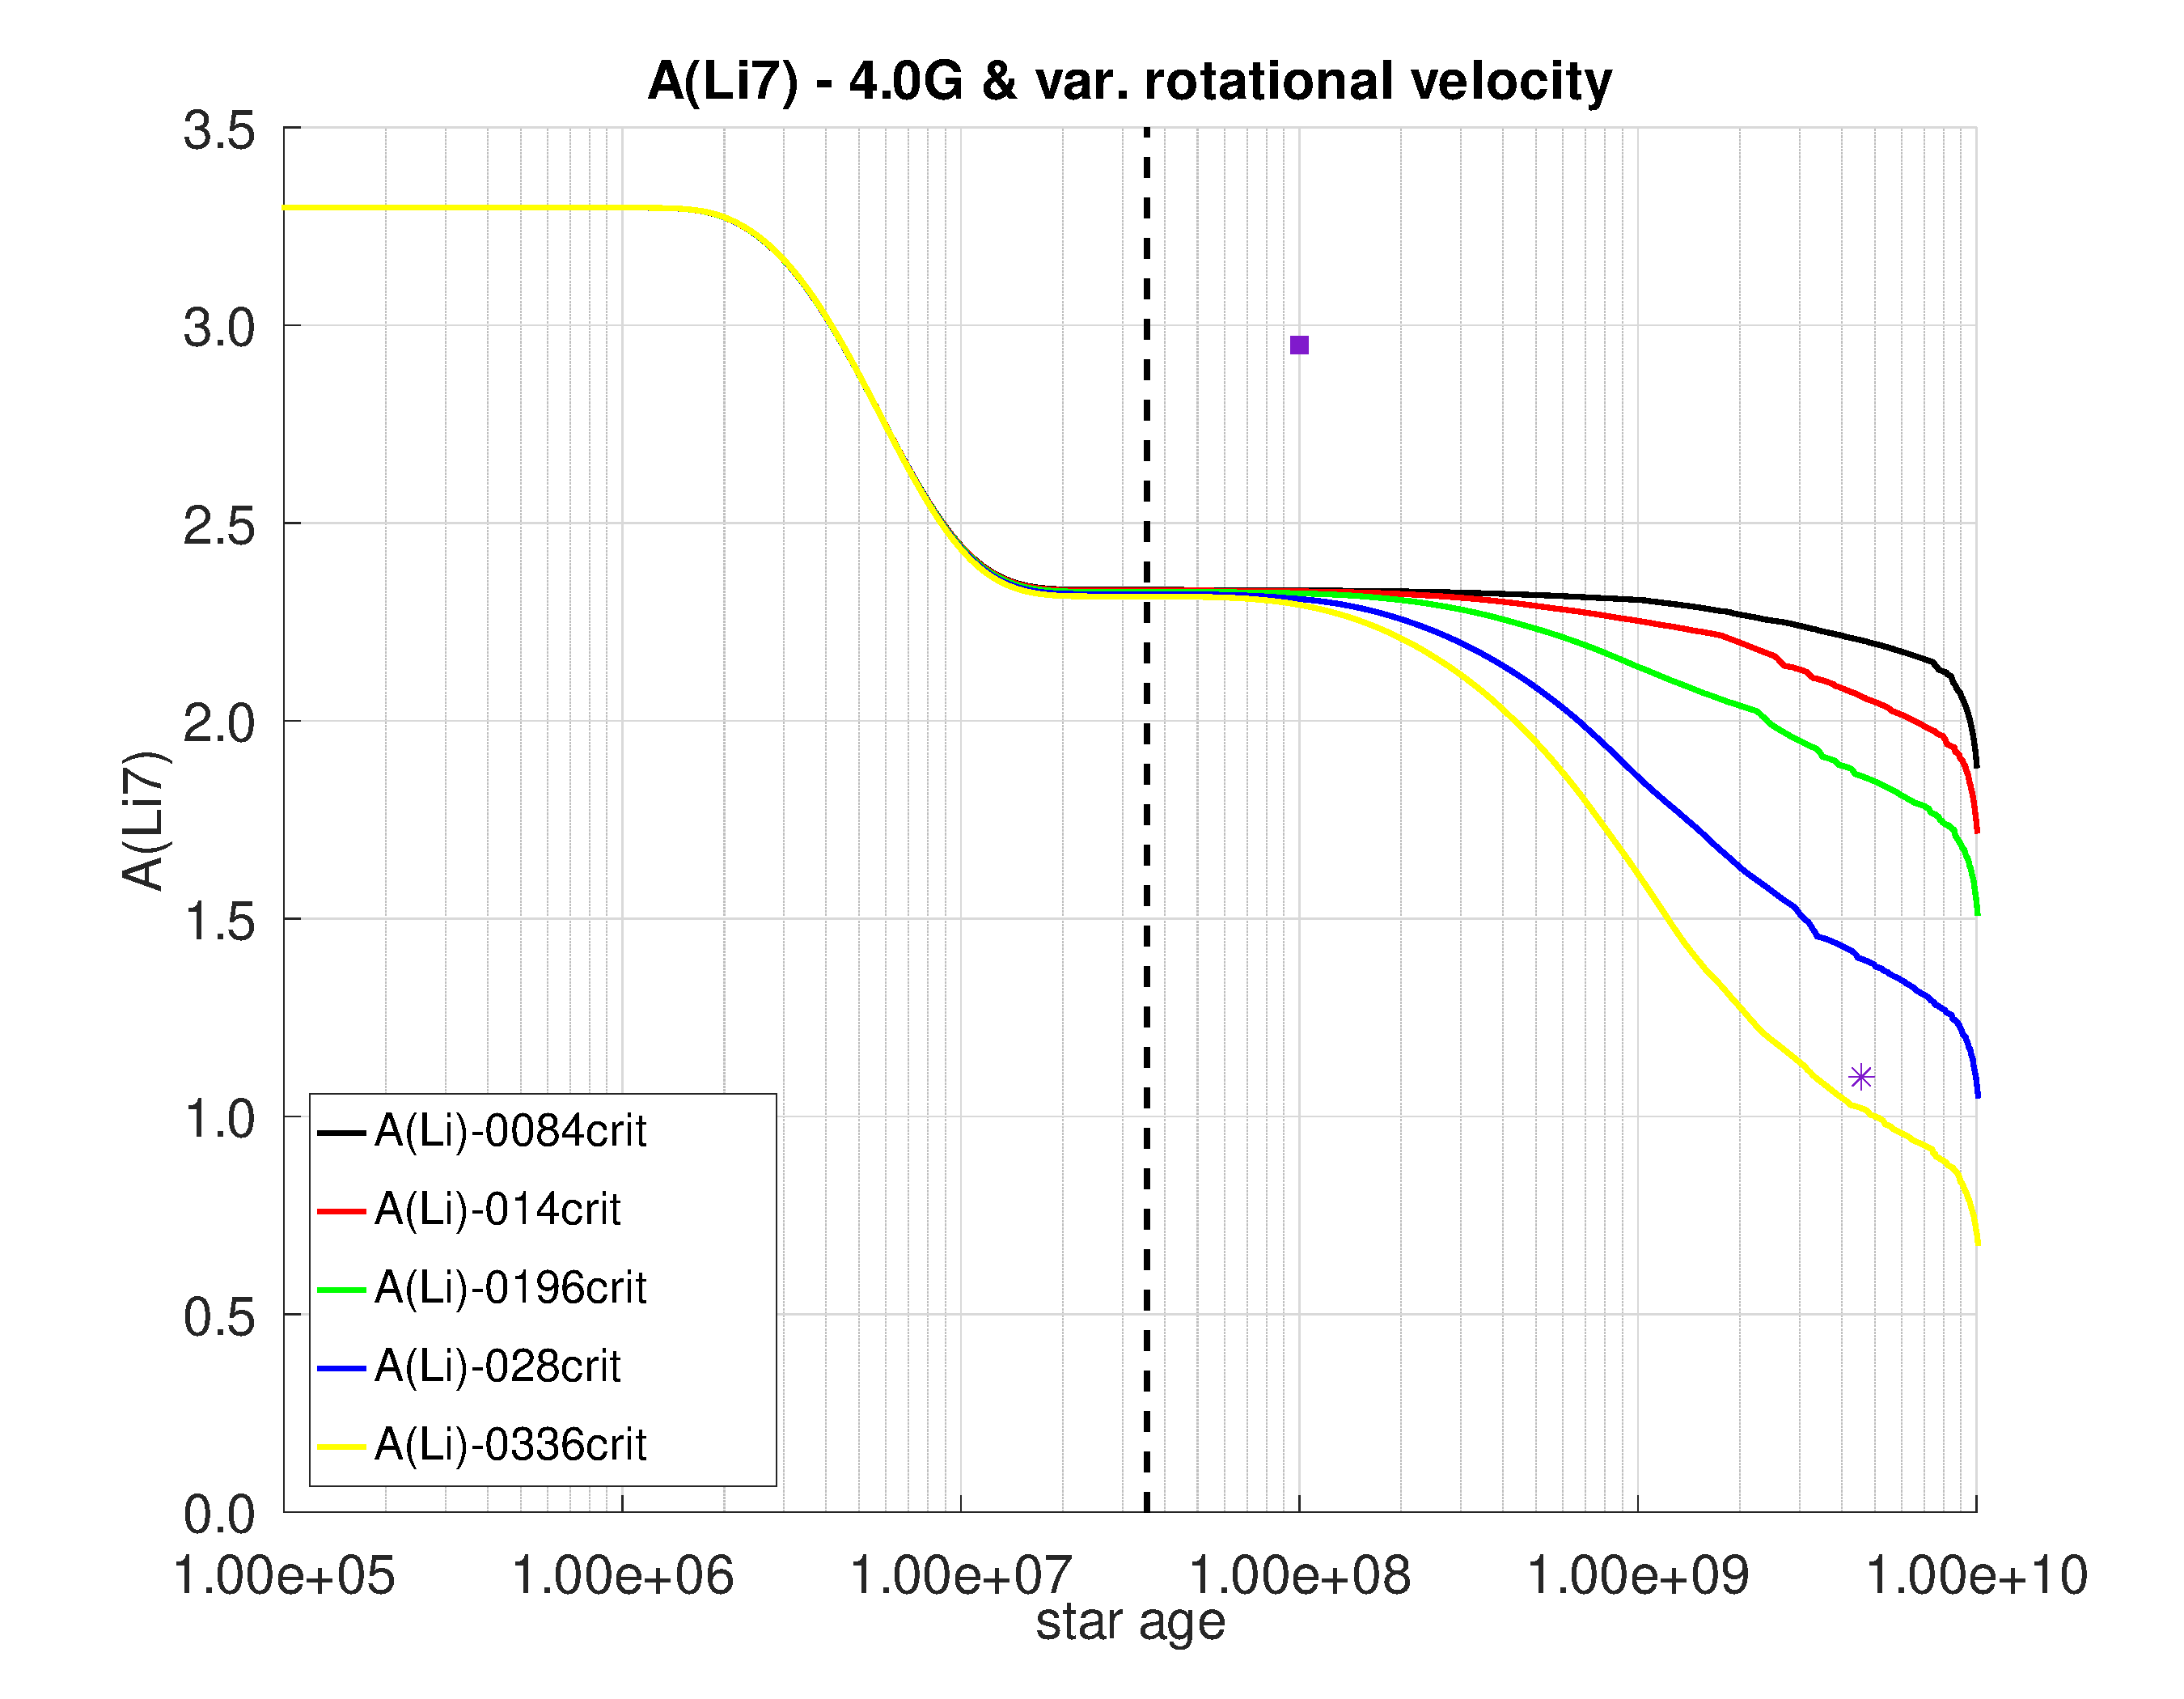
\includegraphics[width=0.7\textwidth]{img/paper1/li_var_vel_4_0g.pdf}
	\caption{Evolución de la abundancia superficial del \isotope[7]{Li} respecto al \isotope[1]{H}, en función del tiempo para varios modelos de 1 $\msun$. Los modelos incluyen un campo magnético con una intensidad de 4G y rotación PMS con $\oomegac$ entre 0,0084 y 0,0336, respectivamente. La estrella púrpura y el cuadrado son la abundancia superficial de Li para el Sol actual \cite{Asplund2009} y el cúmulo de las Pléyades \cite{Sestito2005} respectivamente. La línea vertical discontinua hace referencia a la ZAMS.}
	\label{fig:li_var_vel_4_0g}
\end{figure}

El efecto de la rutina MB puede apreciarse aún más claramente en las Figuras~\ref{fig:rot_vel_4g}, \ref{fig:rot_vel_4g_z1} \& Apéndices \footnote{Los apéndices comprenden una serie de cuadrículas en función del tiempo y para varios modelos de 1 $\msun$ en los que se muestra, por un lado, la evolución de la abundancia superficial del \isotope[7]{Li} respecto al \isotope[1]{H} tanto para intensidades de campo magnético variables como para velocidades angulares y, por otro, la evolución de la velocidad de rotación superficial.}. En estas figuras representamos los perfiles de rotación para la superficie de las estrellas y para el fondo de la envoltura convectiva. Son modelos de 1 $\msun$ inicializados con diferentes velocidades de rotación y considerando la influencia del MB. De forma similar a los perfiles de evolución de $A(\isotope[7]{Li})$ comentados en el párrafo anterior, el efecto de la rutina se hizo visible una vez alcanzada la ZAMS. Si comparamos la evolución de las curvas aquí presentadas con las de la Figura \ref{fig:rot_vel_0g} vemos como la estrella, en lugar de seguir aumentando $\Omega$, comenzó a ralentizarse tras haber alcanzado su máximo en el paso por la ZAMS. Nótese que en este punto las velocidades angulares en la superficie de la estrella y en la ZAMS alcanzaron su máxima diferencia. Por otro lado, el efecto MB hizo que las velocidades angulares entre ambas zonas de la estrella disminuyeran hasta que, para una edad cercana a la del Sol (ver Figura \ref{fig:rot_vel_4g_z1}), la estrella prácticamente rotaba como un sólido rígido. Estos resultados también eran coherentes con los obtenidos por \cite{Eggenberger2010} en cuanto al efecto del campo magnético, en particular su influencia en la pérdida de momento angular, sobre la velocidad de rotación de la estrella.\par

De forma similar, también observamos que los modelos con menor velocidad angular generalmente acababan mostrando valores más altos para la abundancia de Li en la superficie (ver Figuras~ \ref{fig:li_var_vel_4_0g}, \ref{fig:grid_li_var_vel} y \ref{fig:grid_li_var_g}). En ninguno de esos casos obtuvimos valores de Li en la superficie superiores a los mostrados por el modelo sin rotación.\par


\begin{figure}
    \centering
    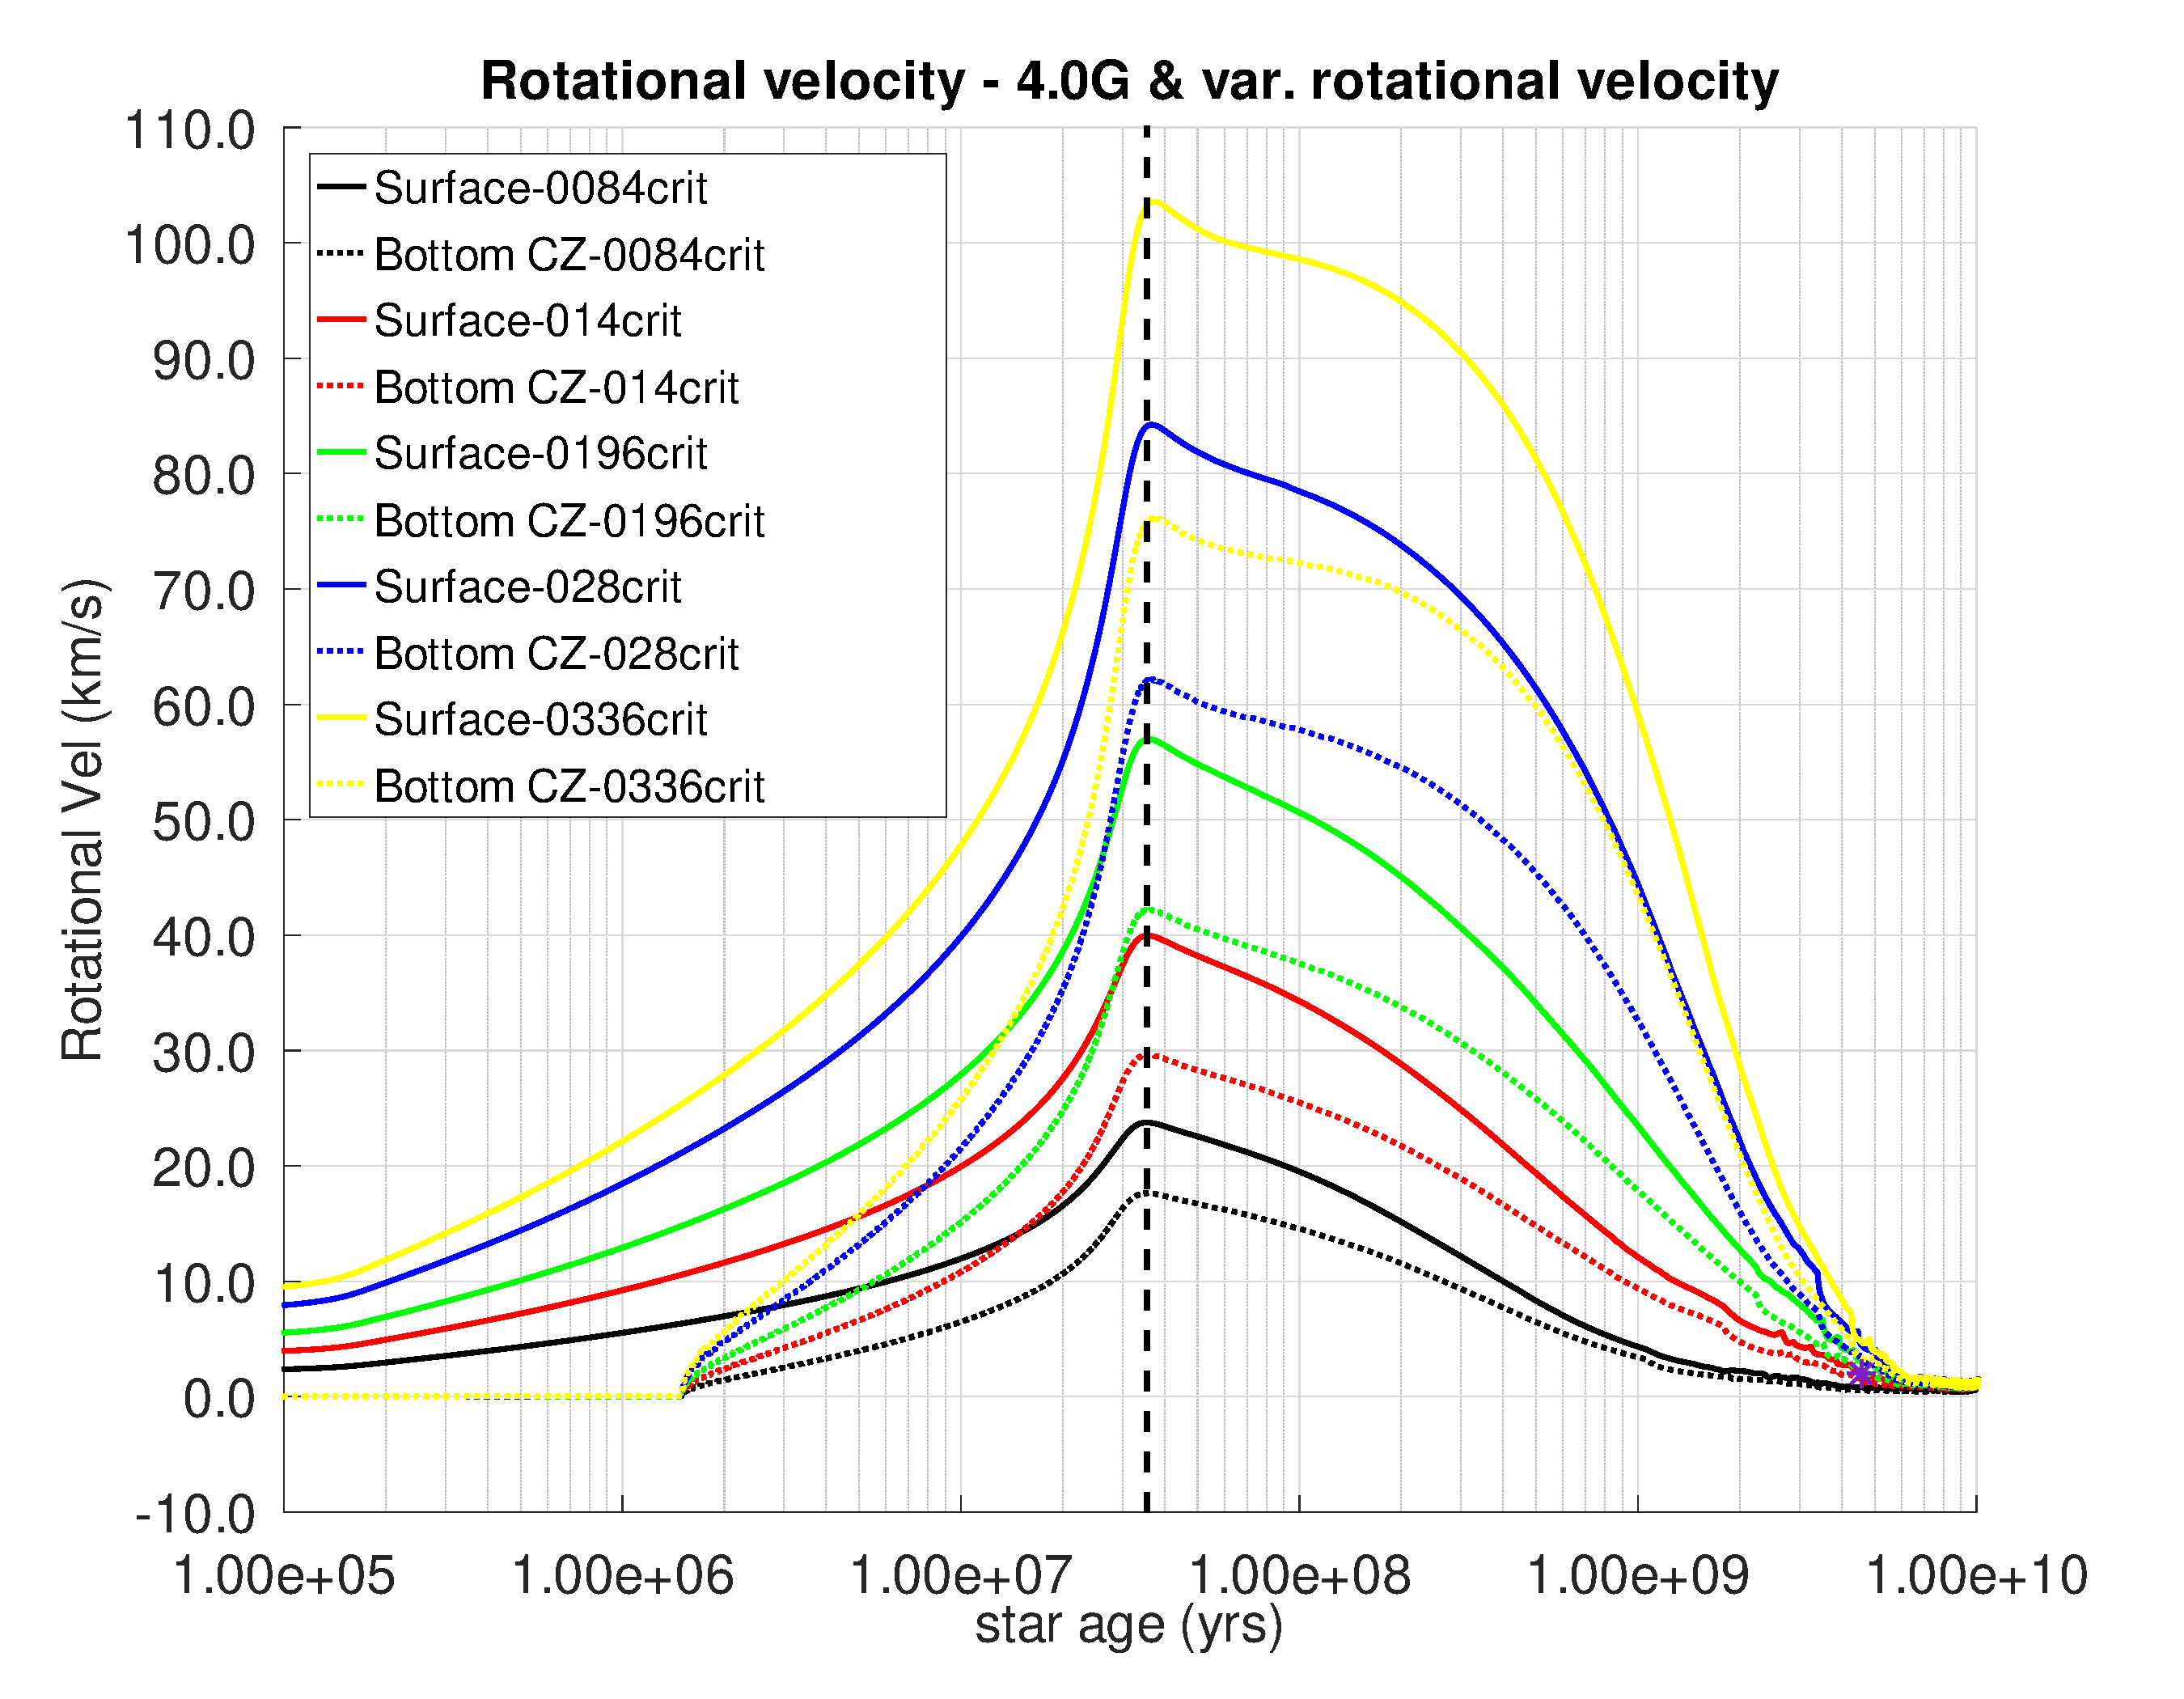
\includegraphics[width=0.7\textwidth]{img/paper1/rot_vel_var_vel_4_0g.pdf}
	\caption{La evolución de la velocidad de rotación de la superficie, en función del tiempo para varios modelos de 1 $\msun$. Los modelos incluyen un campo magnético con una intensidad de 4\,G, rotación PMS con $\oomegac$ entre 0,0084 y 0,0336, respectivamente y MB. La estrella púrpura es la velocidad angular superficial para el Sol actual \cite{Gill2012}. La línea vertical discontinua hace referencia a la ZAMS.}
	\label{fig:rot_vel_4g}
\end{figure}

\begin{figure}
    \centering
    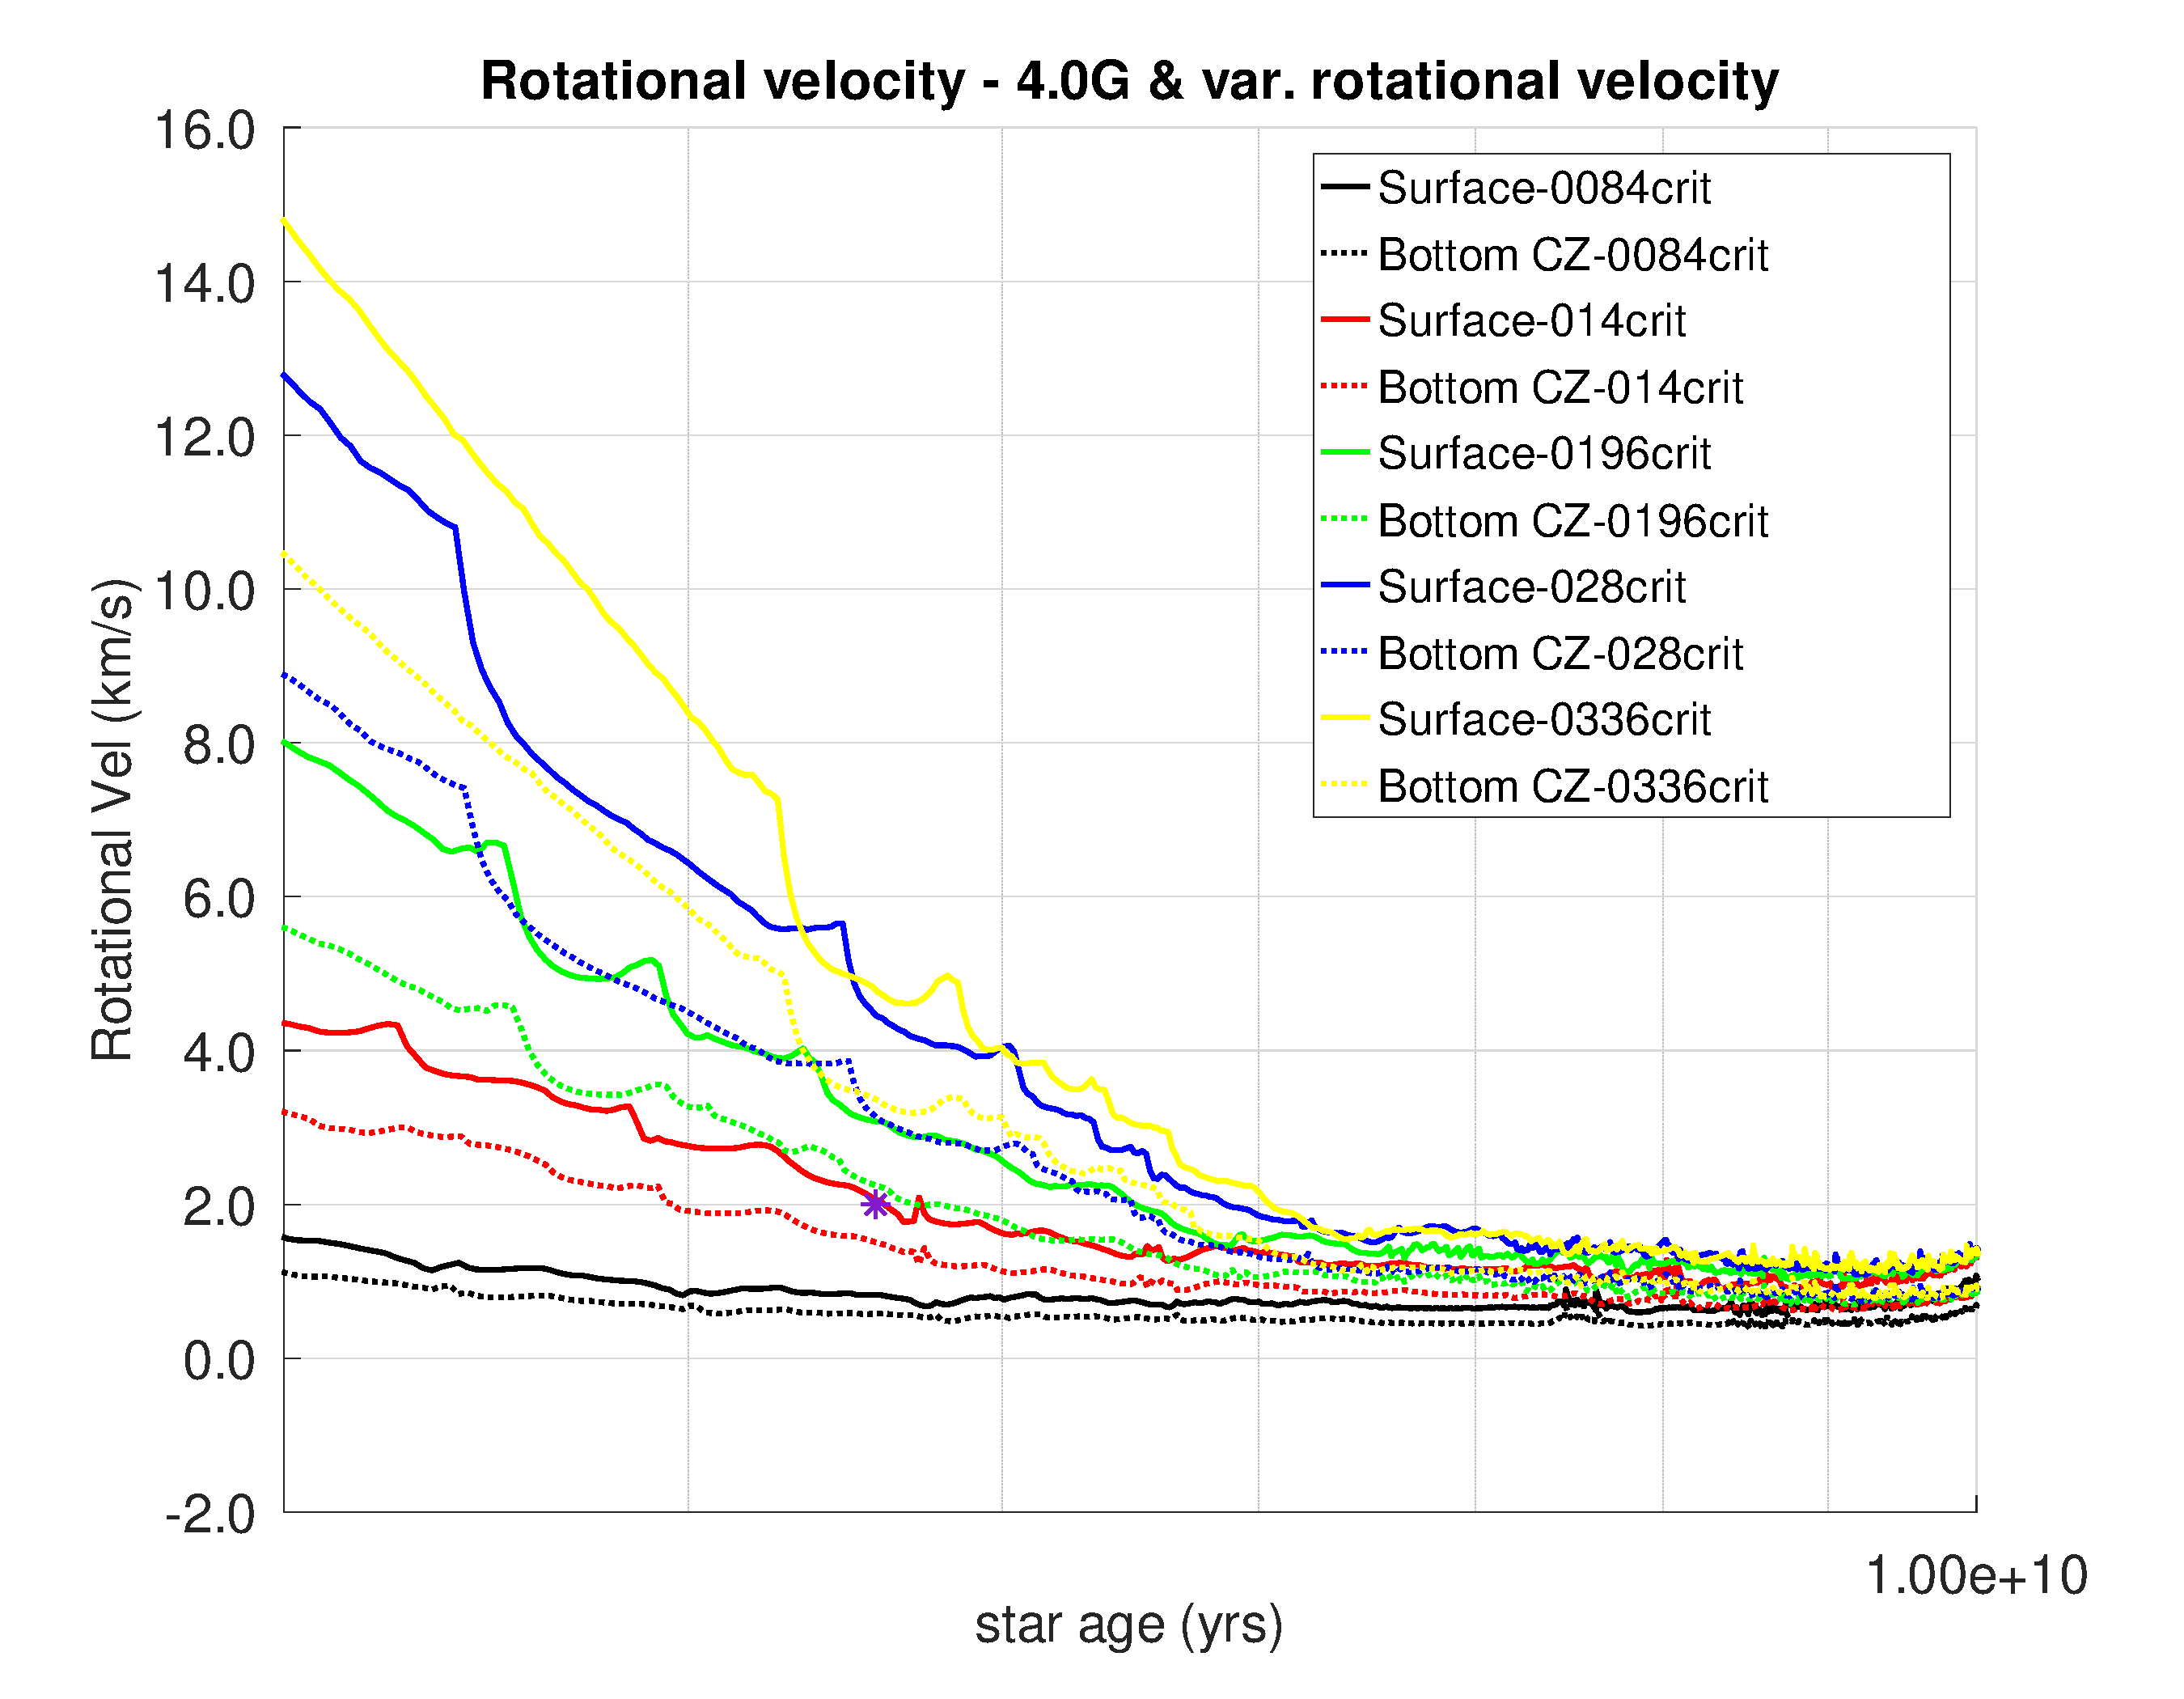
\includegraphics[width=0.7\textwidth]{img/paper1/rot_vel_var_vel_4_0g_z1.pdf}
	\caption{Similar a la Figura \ref{fig:rot_vel_4g} pero ahora mostrando en detalle la velocidad de rotación de la superficie a medida que la estrella se aproxima a TAMS.}
	\label{fig:rot_vel_4g_z1}
\end{figure}

El MB también dejó su huella en el diagrama HR afectando significativamente al $\teff$ de la estrella. Para visualizar este efecto tomamos como referencia la Figura \ref{hr_vc_0336_var_g_z1} en la que todos los modelos se iniciaron con el mismo valor $\oomegac=0,0336$ pero la intensidad del campo magnético simulado fue diferente. Obsérvese que los modelos con MB produjeron estrellas más calientes debido a su influencia. La menor velocidad con la que giraba la estrella debido al efecto MB provocó el aumento del $\teff$, siendo esta diferencia de prácticamente 95K entre los modelos simulados con 0.0G y 5.0G respectivamente para $log(\llsun)=0$.

\begin{figure}
    \centering
    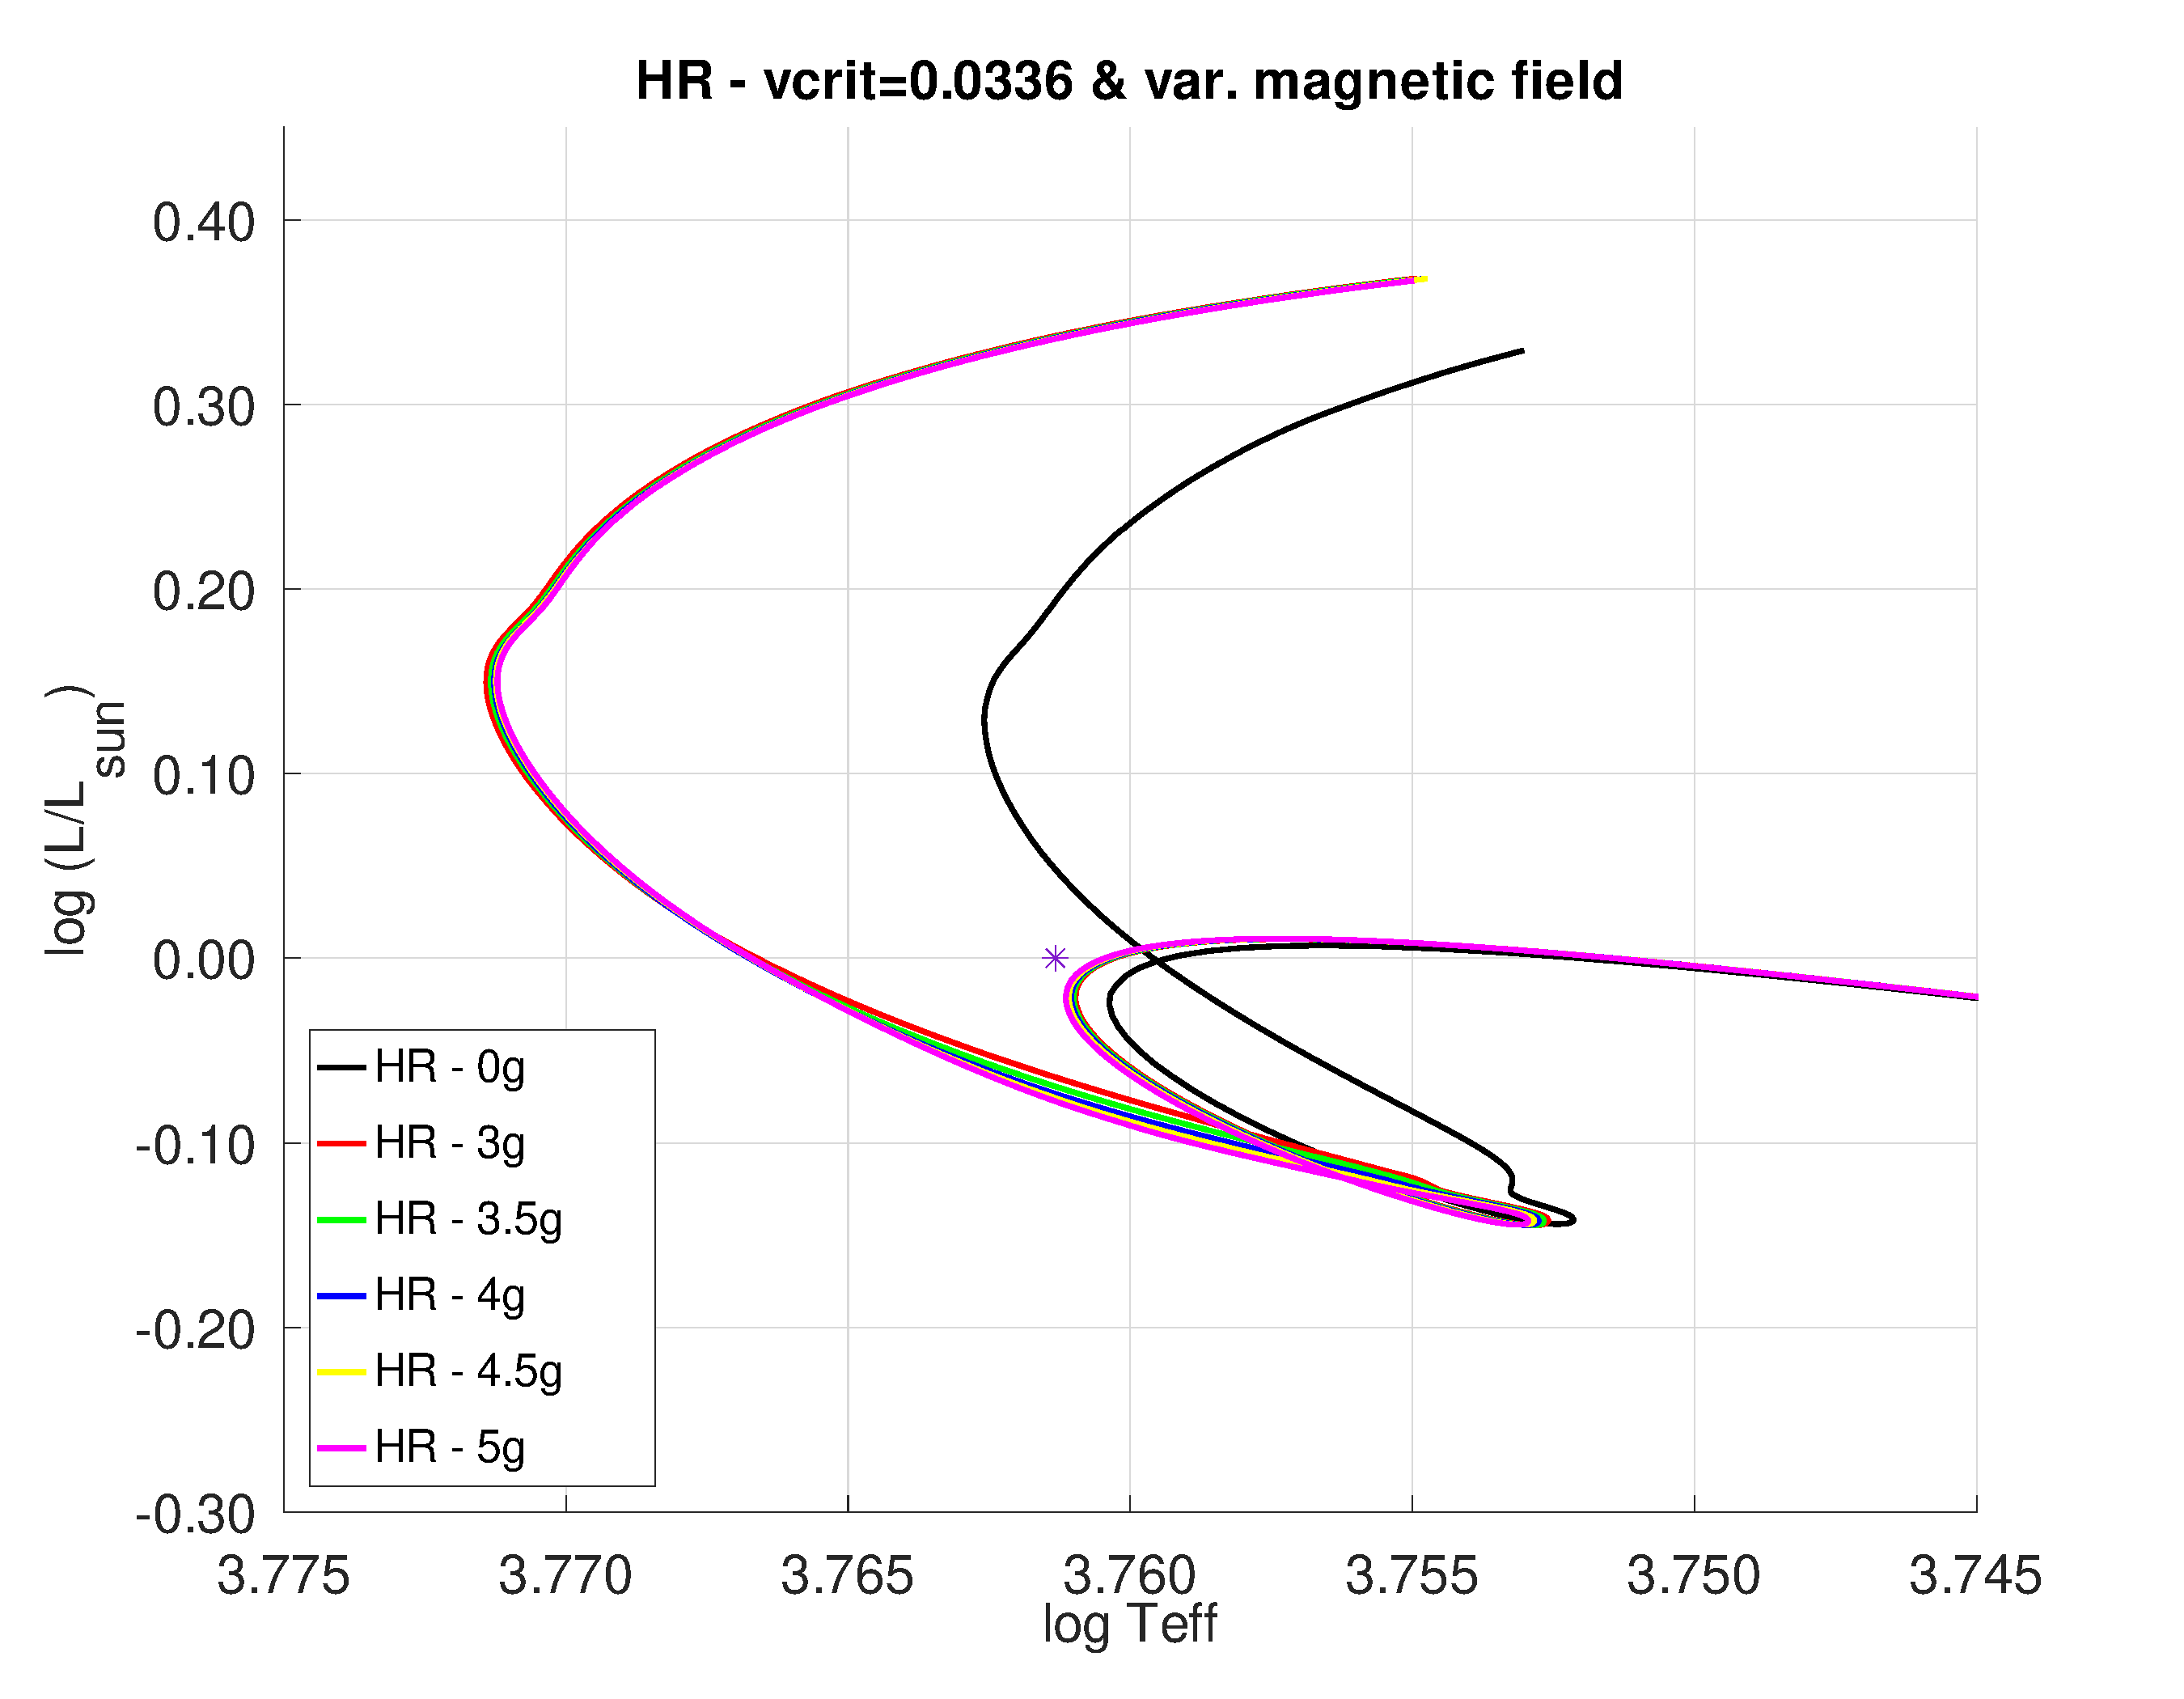
\includegraphics[width=0.7\textwidth]{img/paper1/hr_vc_0336_var_g_z1.pdf}
	\caption{Similar a la Figura \ref{fig:hr_var_vel_0g} pero ahora mostrando en detalle los efectos del frenado magnético en las trayectorias evolutivas para diferentes intensidades de campo magnético y $\oomegac=0.0336$. La presencia de un campo magnético produce estrellas más calientes debido a la influencia del frenado magnético en la velocidad de rotación de la estrella.}
	\label{hr_vc_0336_var_g_z1}
\end{figure}

Como se describe en la sección \ref{sec_mesh}, la rutina MB distribuyó la cantidad total de AML calculada según la Ec.~\ref{eq:k_jdot} entre las distintas capas que componían la CZ. En la Figura \ref{fig:cz_vc_028_var_b} podemos observar la evolución de la CZ más externa normalizada con respecto al radio de la estrella para varios modelos de 1 $\msun$. Todos los modelos se inicializaron con $\oomegac=0.0336$ e intensidades de campo magnético que variaban entre 0.0G y 5.0G. De acuerdo con los modelos establecidos de evolución estelar, en una estrella de tipo solar la CZ cubre prácticamente toda ella durante gran parte del PMS. A medida que se aproxima a la ZAMS, la CZ va disminuyendo como consecuencia de la aparición de un núcleo radiativo y mantiene un radio aproximadamente constante hasta la etapa final de la MS. En este punto aumenta significativamente como respuesta a la expansión generalizada del radio de la estrella. En cuanto al efecto deL MB sobre el tamaño de la CZ, observamos que a medida que aumentaba la intensidad del campo magnético, el tamaño de la CZ disminuía (véase la figura \ref{fig:cz_vc_028_var_b_z1_new}). El núcleo radiativo se desplazó hacia el exterior para incluir una fracción cada vez mayor de la masa estelar, haciendo que la temperatura en la base de la CZ cayera por debajo de $\tli$. Este efecto fue más evidente durante la MS. La disminución del tamaño de la CZ estuvo en consonancia con el hecho de que se destruyera menos Li haciendo que menos material estelar alcanzara zonas con temperaturas superiores a $\tli$.\par

\begin{figure}
    \centering
    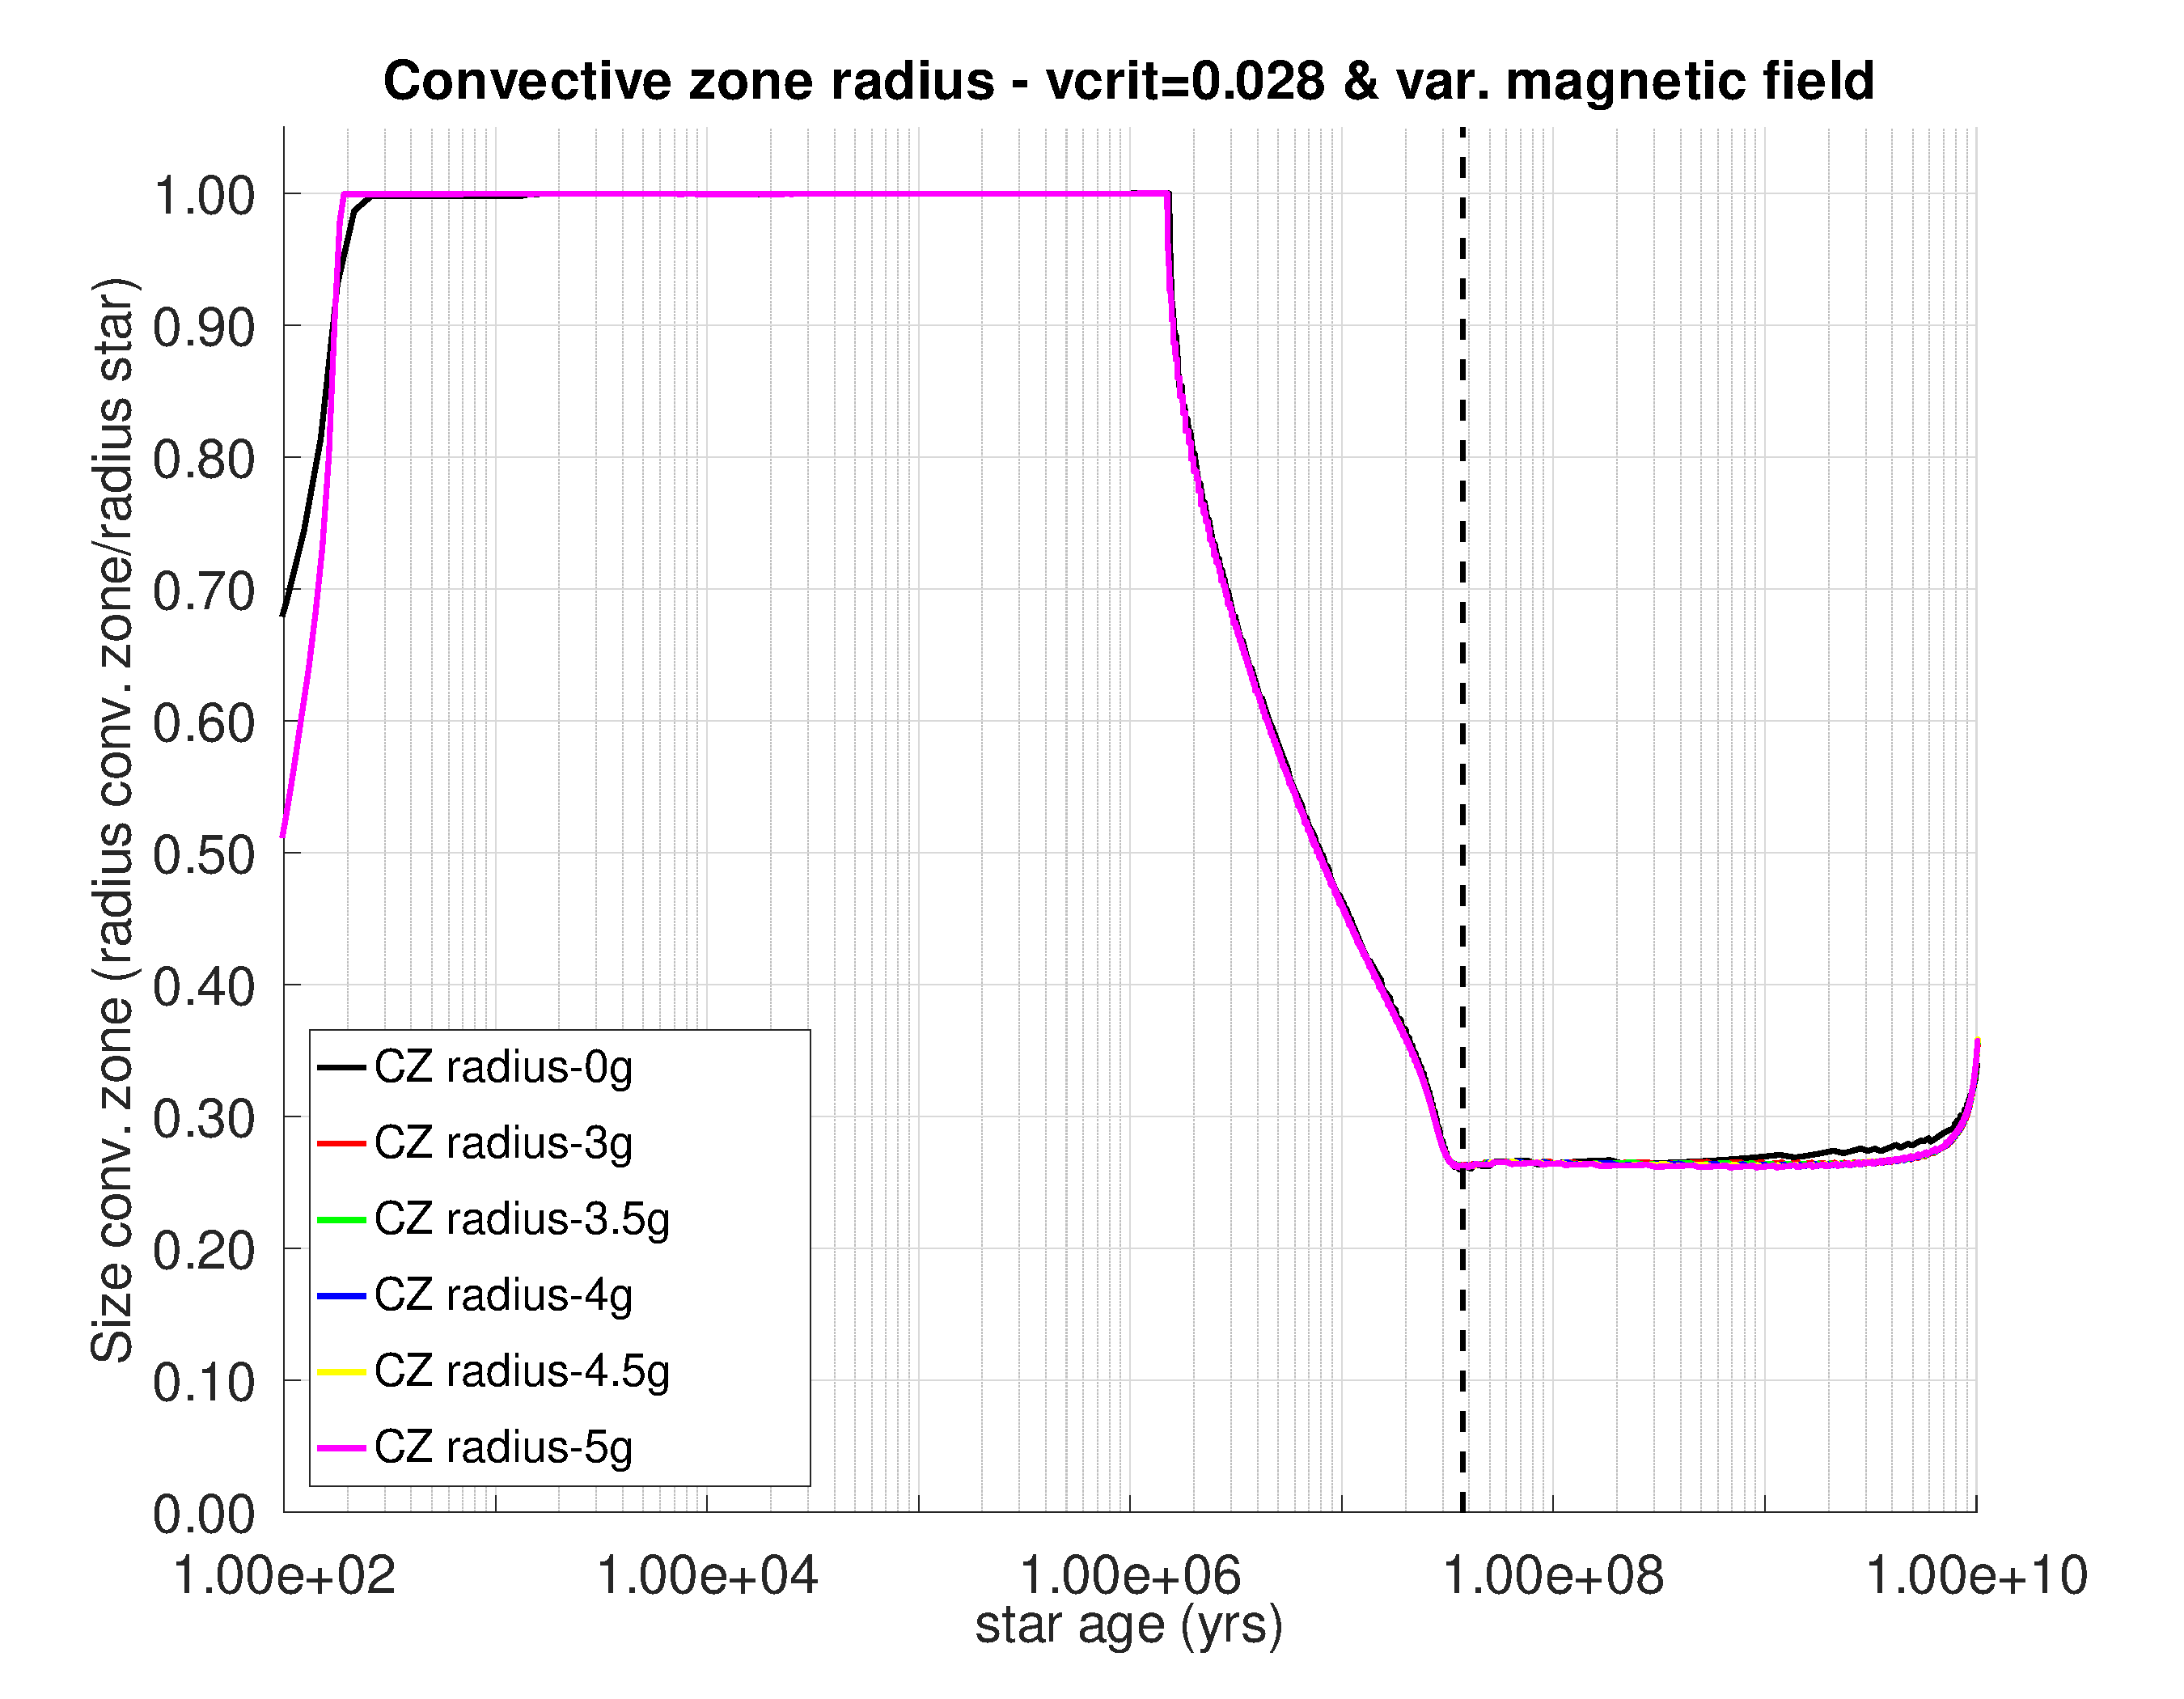
\includegraphics[width=0.7\textwidth]{img/paper1/cz_vc_028_var_g.pdf}
	\caption{Evolución del tamaño de la zona convectiva en función del tiempo para varios modelos de 1 $\msun$. Todos los modelos se inicializaron con $\oomegac=0.0336$ y las intensidades de campo magnético varían entre 0.0G y 5.0G. La línea vertical discontinua hace referencia a la ZAMS.}
	\label{fig:cz_vc_028_var_b}
\end{figure}

En la Figura \ref{fig:mdot_vc_028_var_b} podemos ver la evolución de $\Dot{M}$ durante PMS y MS para varios modelos de 1 $\msun$. Todos los modelos se inicializaron con $\oomegac=0.0336$ e intensidades de campo magnético que variaban entre 0.0G y 5.0G. En las primeras etapas del PMS fue donde se concentró la mayor pérdida de masa, que fue disminuyendo a medida que se acercaba a la ZAMS. Como la estrella también disminuyó su radio durante la PMS, aumentó $\Omega$ obedeciendo al principio de conservación del AM. Al llegar a la ZAMS, el radio estelar se mantuvo más o menos estable durante gran parte de la MS (excepto en su etapa final, véase la figura \ref{fig:mdot_vc_028_var_b_z1}), pero siguió perdiendo masa mientras aumentaba $\Omega$, aunque de forma menos agresiva si lo comparamos con la PMS. Sin embargo, como consecuencia tanto de la aparición del núcleo radiativo durante el seguimiento de Henyey como de la existencia de una CZ (véase la figura \ref{fig:mb_act_var_vel_vc_028}), se activó la rutina MB, provocando que la velocidad angular de la estrella comenzara a disminuir a lo largo de toda la MS. Cuanto más intenso es el campo magnético, mayor es el efecto de frenado.\par 

\begin{figure}
    \centering
    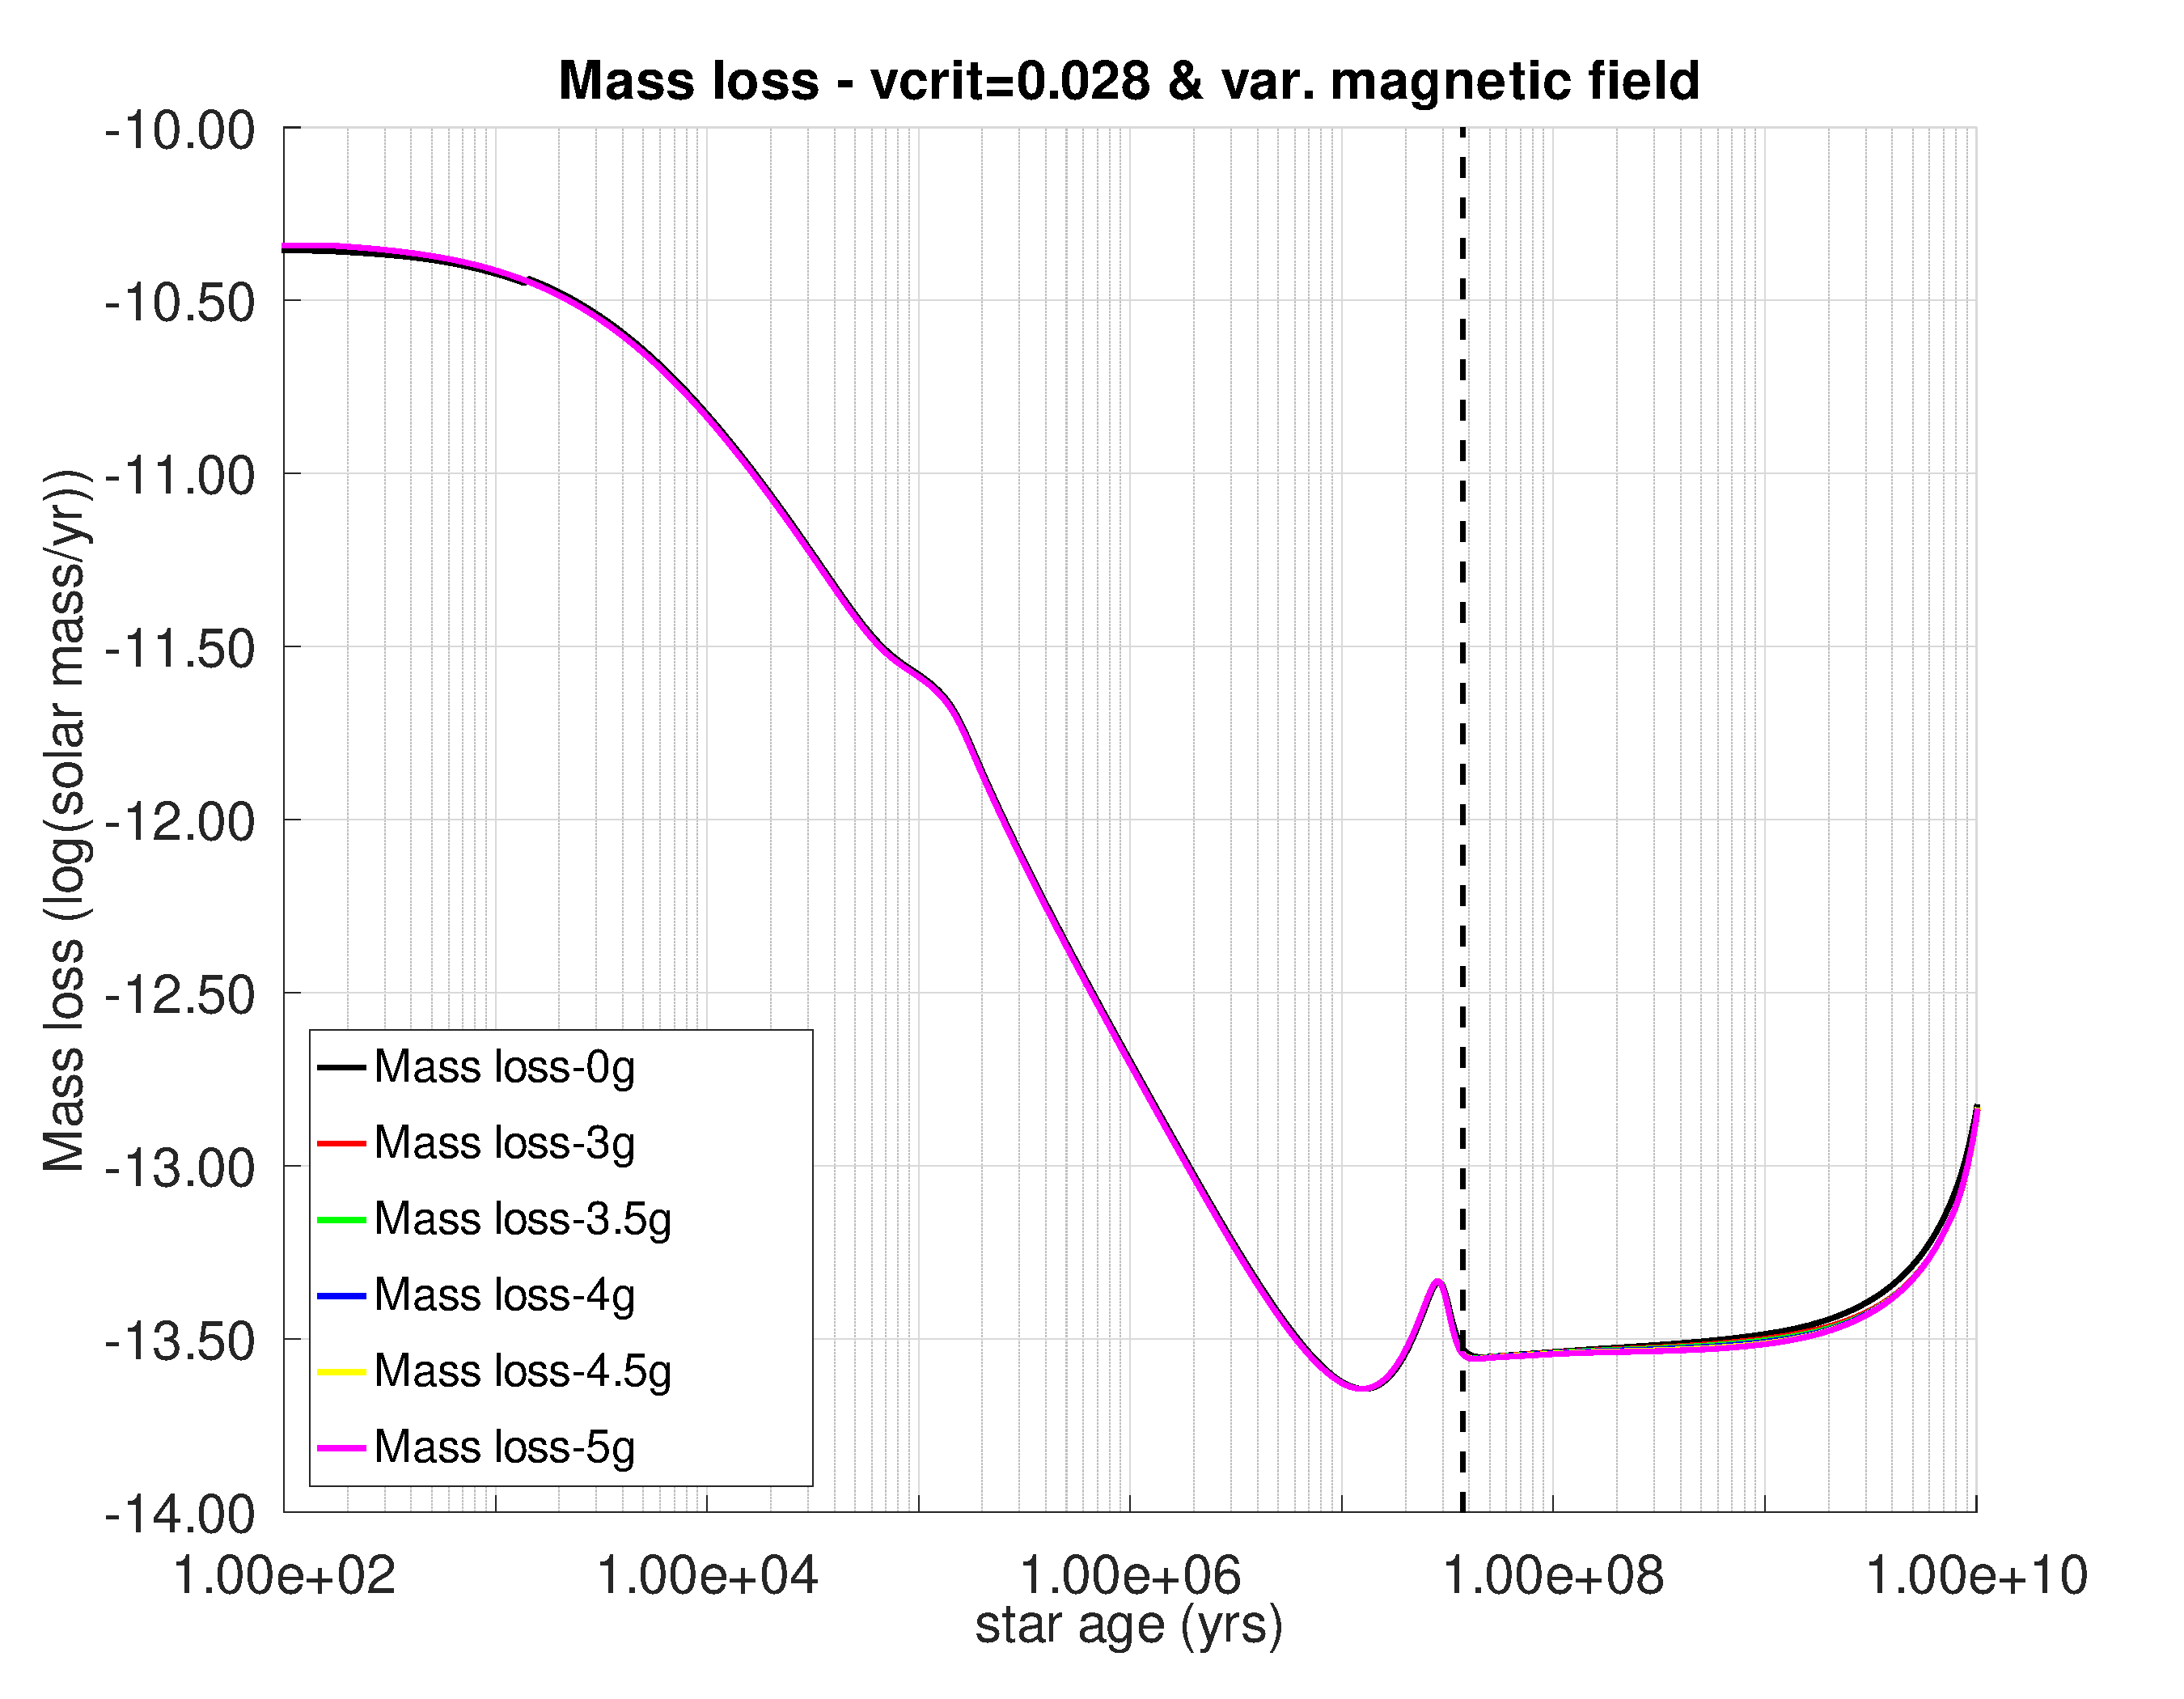
\includegraphics[width=0.7\textwidth]{img/paper1/mdot_vc_028_var_g.pdf}
	\caption{Evolución de la pérdida de masa $\Dot{M}$ en función del tiempo para varios modelos de 1 $\msun$. Los modelos incluyen diferentes intensidades de campo magnético entre 0.0G y 5.0G y rotación PMS con $\oomegac=0.028$. La línea vertical discontinua hace referencia a la ZAMS.}
	\label{fig:mdot_vc_028_var_b}
\end{figure}

\begin{figure}
    \centering
    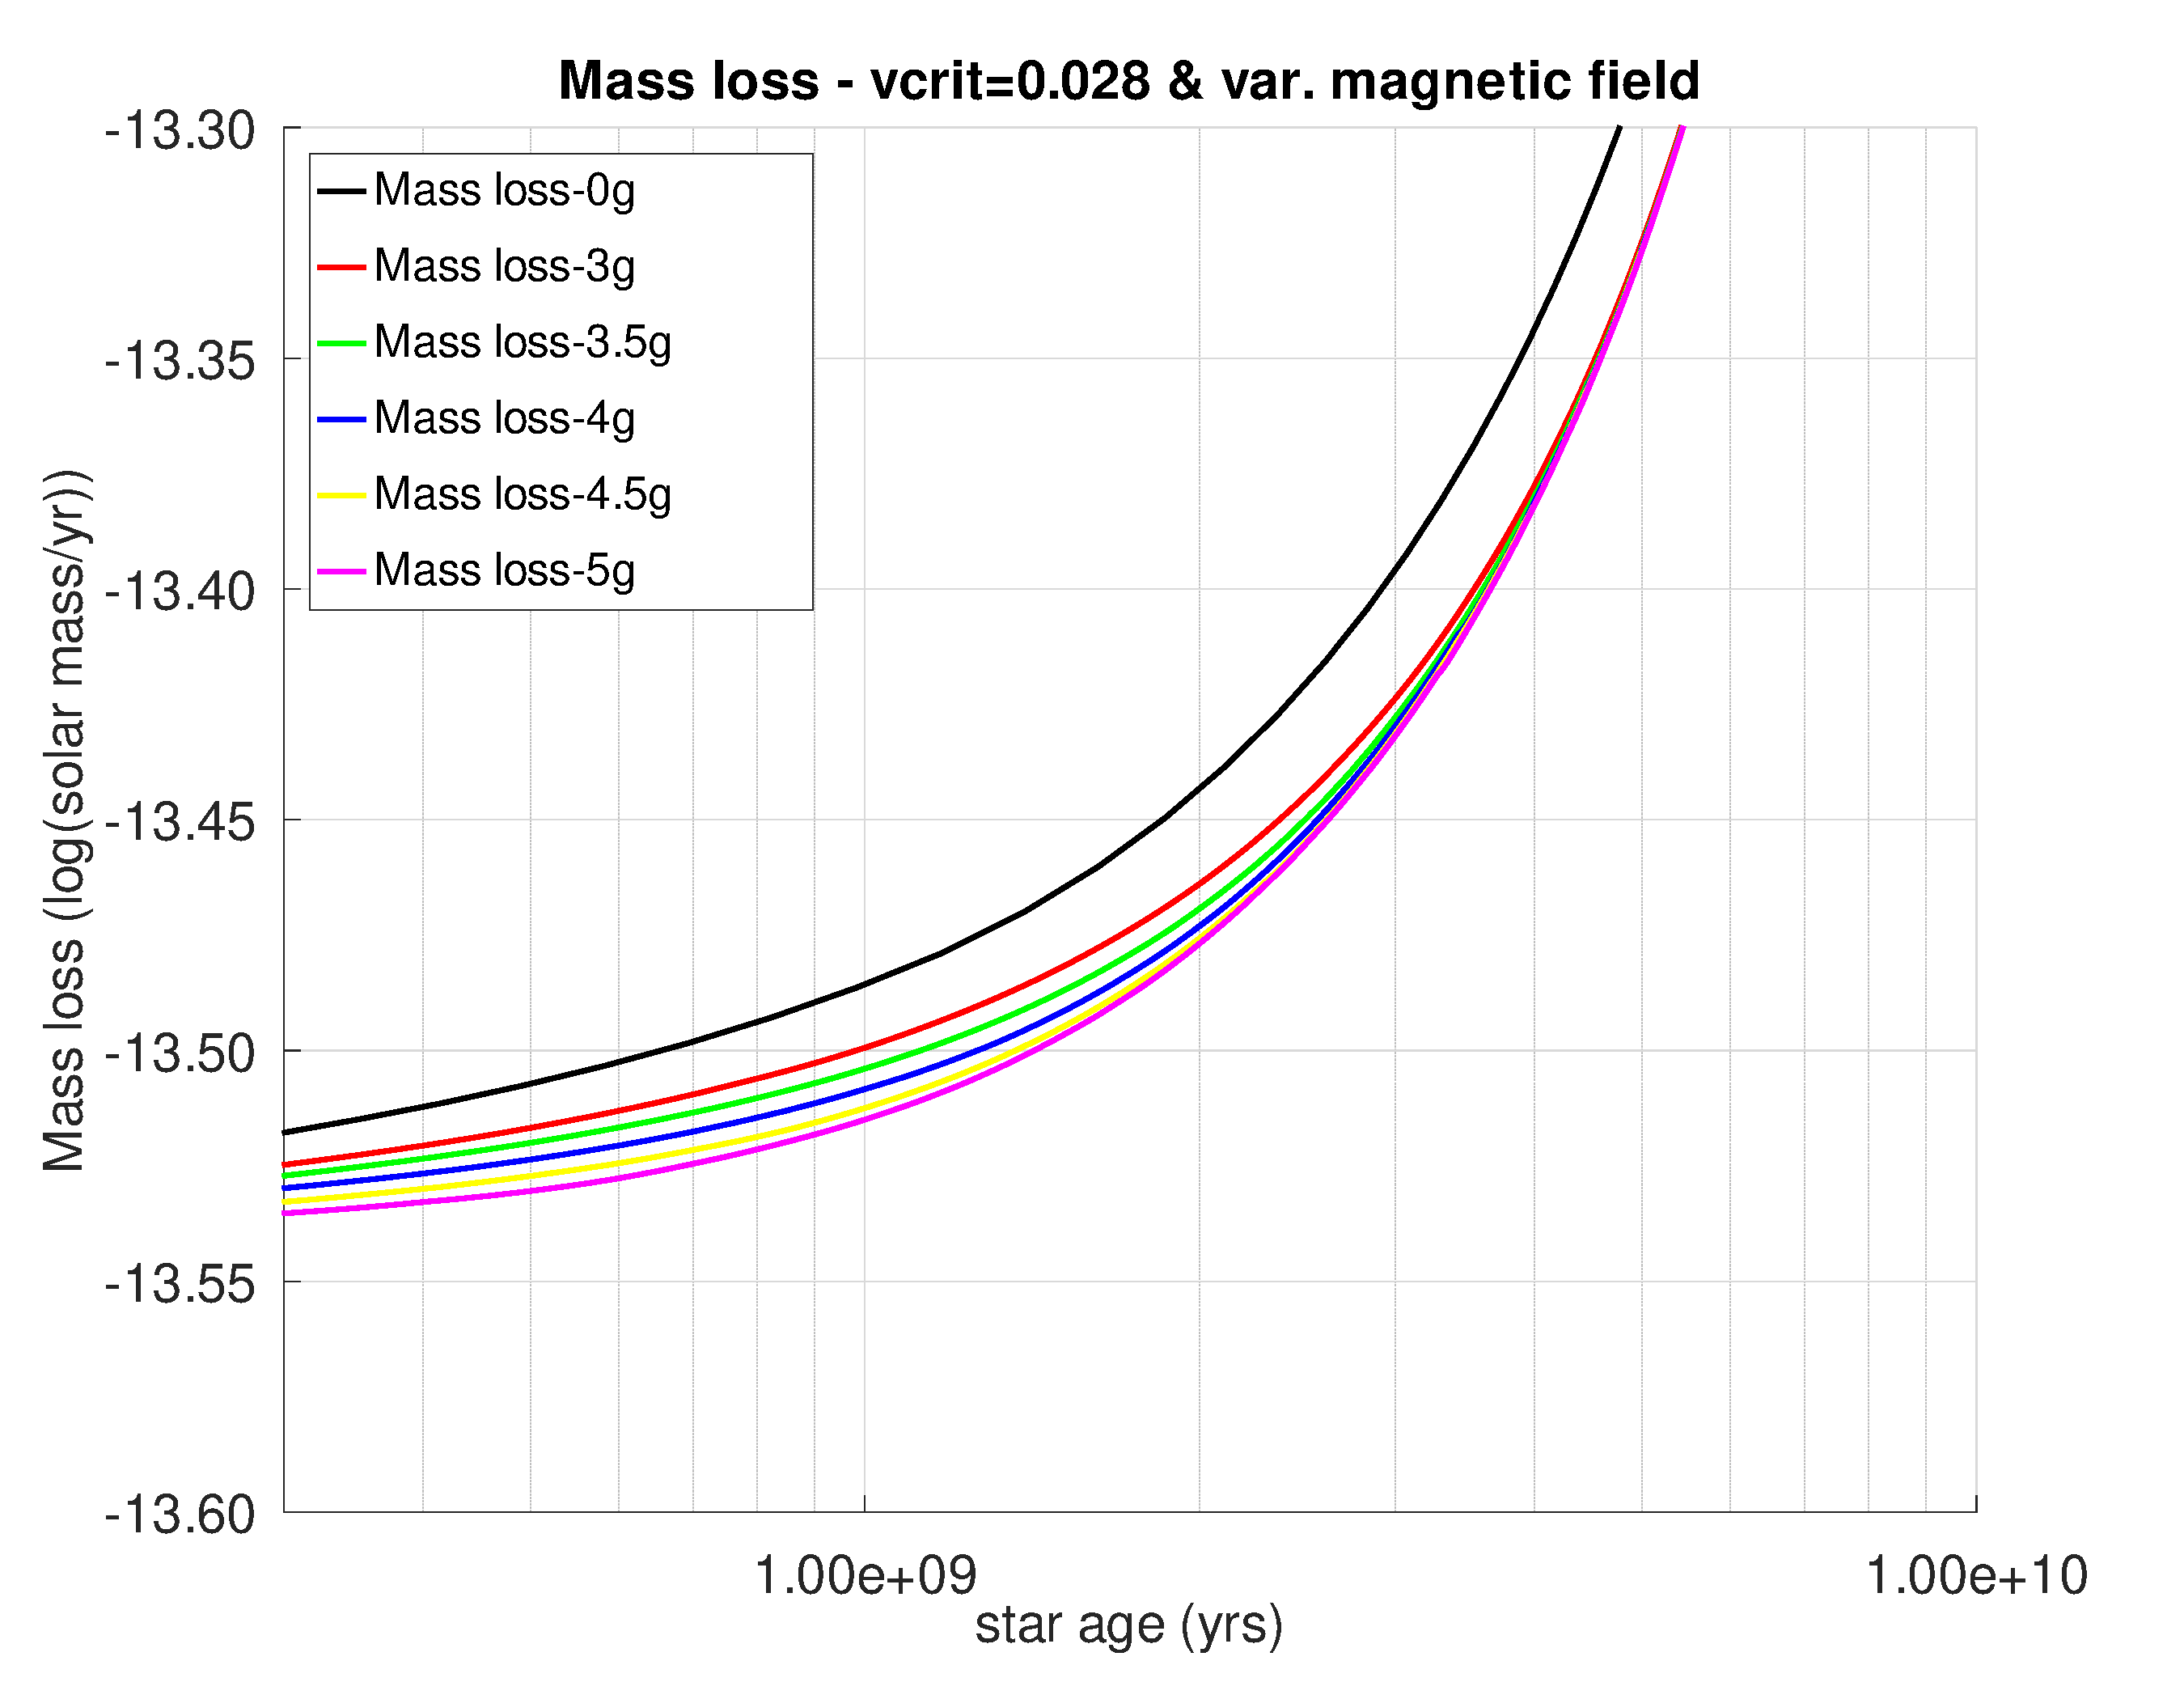
\includegraphics[width=0.7\textwidth]{img/paper1/mdot_vc_028_var_g_z1.pdf}
	\caption{La evolución de la pérdida de masa $\Dot{M}$ a medida que la estrella se acerca a TAMS, en función del tiempo para varios modelos de 1 $\msun$. Los modelos incluyen una intensidad de campo magnético variable entre 0.0G y 5.0G y rotación PMS con $\oomegac=0.028$. Cuanto más intenso sea el campo magnético, menor será $\Dot{M}$.}
	\label{fig:mdot_vc_028_var_b_z1}
\end{figure}

\begin{figure}
    \centering
    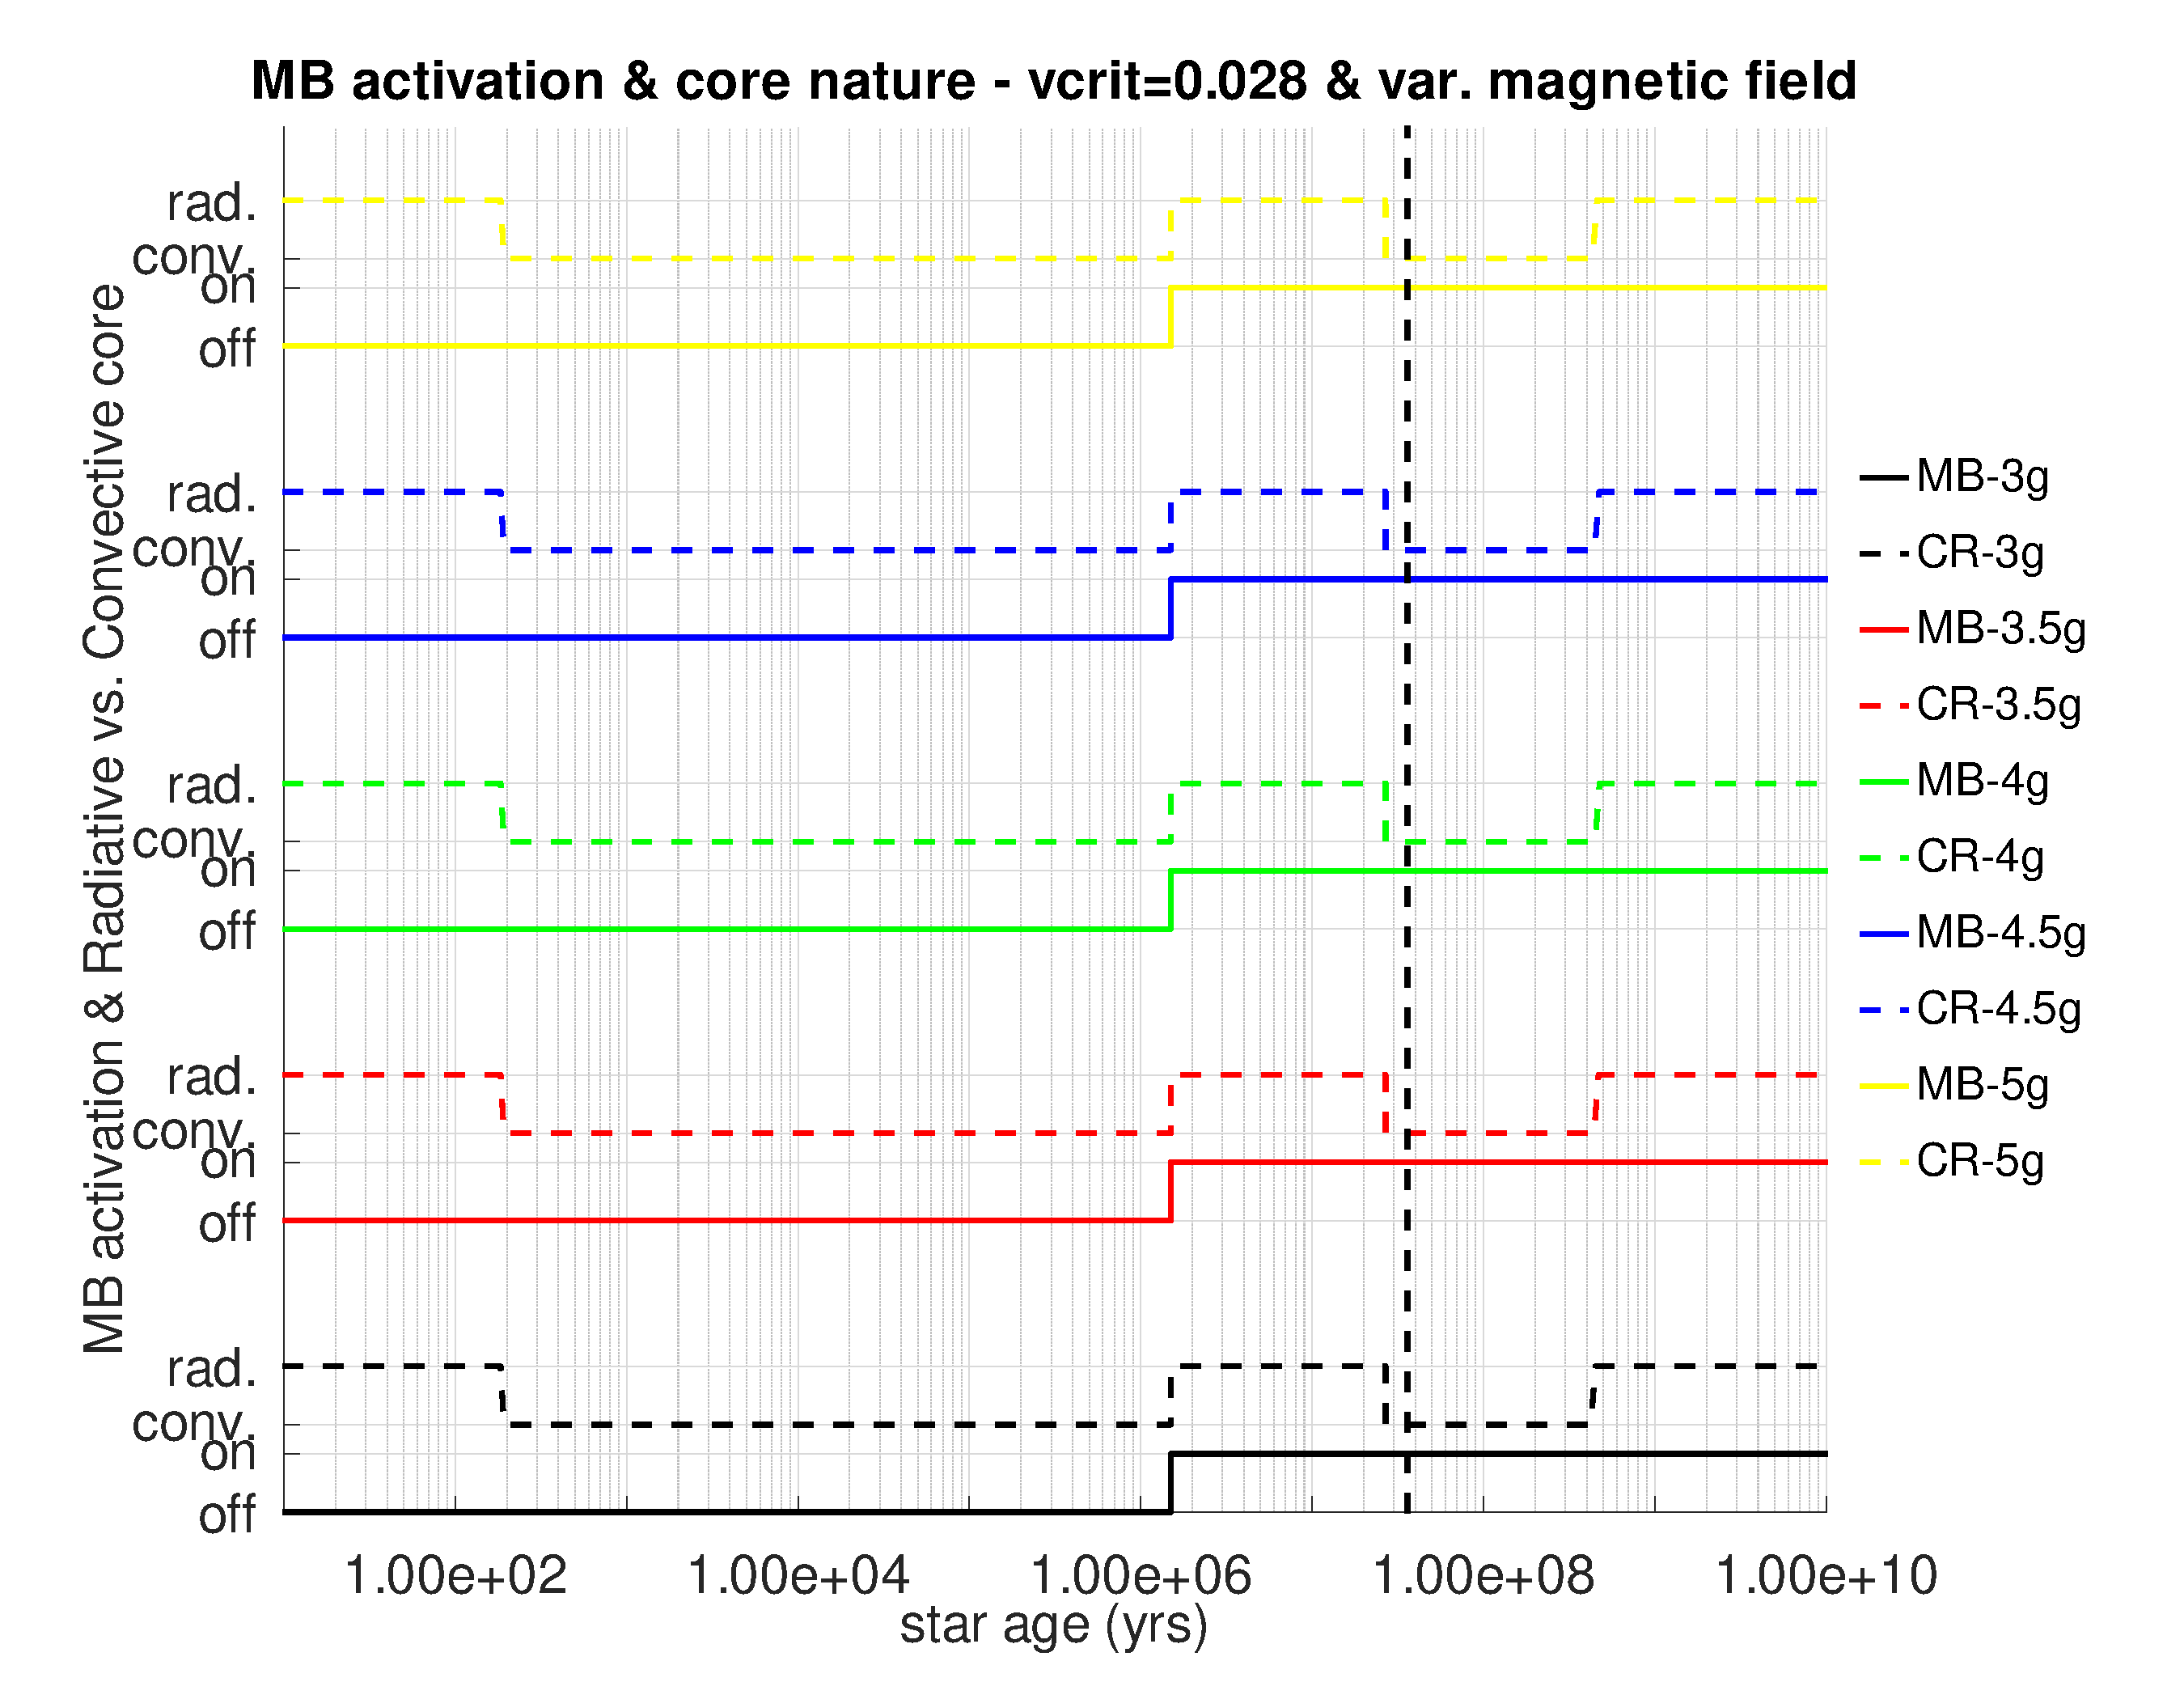
\includegraphics[width=0.7\textwidth]{img/paper1/mb_act_vc_028_var_g.pdf}
	\caption{La activación de la rutina de frenado magnético en función de la presencia de un núcleo radiativo. Los modelos incluyen un campo magnético con una intensidad comprendida entre 0.0G y 5.0G y una rotación PMS con $\oomegac=0.0228$. Las líneas continuas señalan la activación (on) y desactivación (off) de la rutina de frenado magnético. Las líneas horizontales discontinuas informan sobre la naturaleza del núcleo de la estrella: radiativo (rad) o convectivo (conv). Por decisión de implementación, una vez activada la rutina, permanece activada incluso si la naturaleza del núcleo de la estrella cambia a convectiva. La línea vertical discontinua hace referencia a la ZAMS.}
	\label{fig:mb_act_var_vel_vc_028}
\end{figure}

\subsection{Evolución alternativa del Li con MB}
Hasta este punto, las simulaciones de los diferentes modelos se basaron en la parametrización recogida en la Tabla \ref{tab:phy_mesa}, que a su vez fue adoptada de \cite{Choi2016}. Si recordamos la evolución del Li mostrada en las Figuras \ref{fig:li_var_vel_0g} y \ref{fig:li_var_vel_4_0g}, destacamos que en ambos casos se quemaba demasiado Li antes de llegar a la ZAMS y, por tanto, no coincidía con la abundancia media de Li en superficie de las Pléyades. Por otro lado, utilizando una parametrización ligeramente distinta de la empleada hasta ahora en la que los parámetros de convección y \textit{overshooting} se han reajustado según la Tabla \ref{tab:phy_alt_mesa}, las simulaciones pudieron reproducir con mayor fidelidad tanto las abundancias de Li del cúmulo de las Pléyades como las del Sol (véase la Figura \ref{fig:li_3_0g_0314vc}).\par

\begin{table}
	\centering
	\caption{Alternative MTL and overshooting parameters.}
	\label{tab:phy_alt_mesa}
	\begin{tabular}{ll} 
		\hline
		Parameter & Adopted prescriptions and values\\
		\hline
		Convection & MLT + Ledoux, $\alpha_\mathrm{MLT}$ = 1.70\\
		Overshoot & time-dependent, diffusive, $f_\mathrm{ov,core}=0.016$, \\ & $f_\mathrm{ov,sh}=0.002$\\
		\hline
	\end{tabular}
\end{table}

\begin{figure}
    \centering
    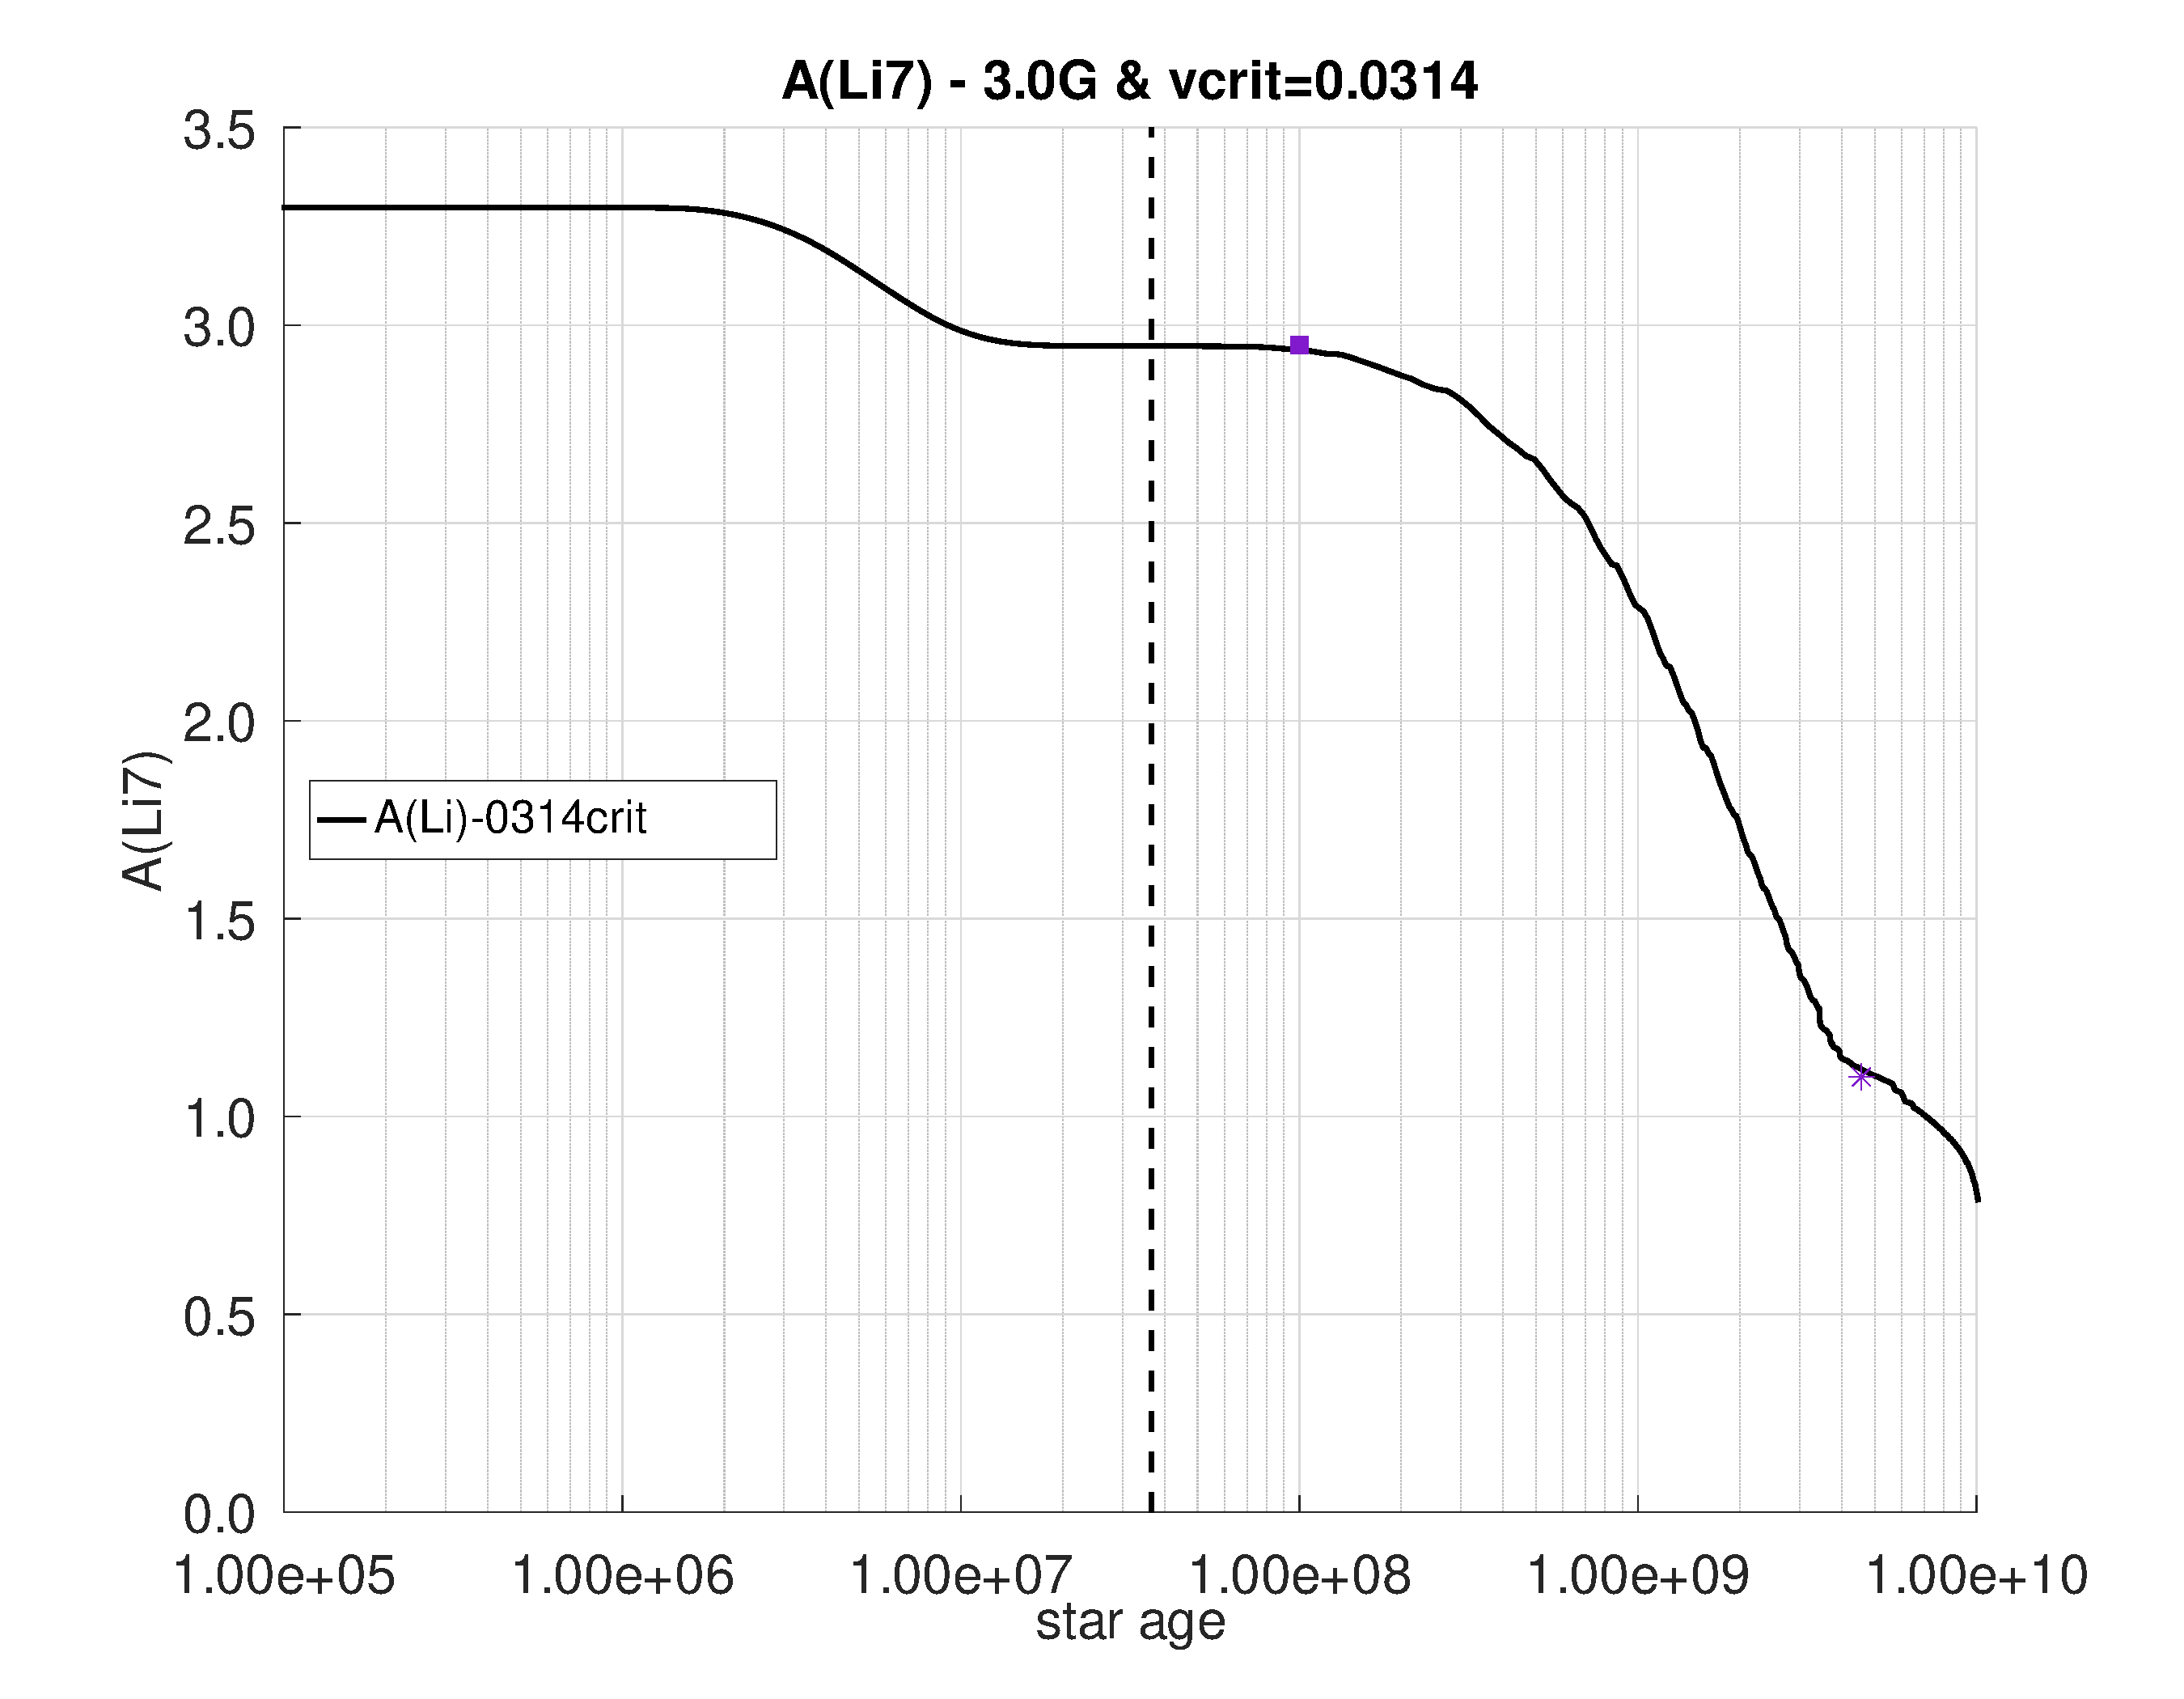
\includegraphics[width=0.7\textwidth]{img/paper1/li_3_0g_0314vc.pdf}
	\caption{La evolución de la abundancia superficial del \isotope[7]{Li} respecto al \isotope[1]{H}, en función del tiempo para un modelo de 1 $\msun$. El modelo incluye un campo magnético con una intensidad de 3G y rotación PMS con $\oomegac= 0.0314$, respectivamente. Los parámetros MLT y overshooting se han fijado en $\alpha_\mathrm{MLT}=1.70$, $f_\mathrm{ov,core}=0.016$, $f_\mathrm{ov,sh}=0.002$. La estrella púrpura y el cuadrado son la abundancia superficial de Li para el Sol actual \cite{Asplund2009} y el cúmulo de las Pléyades \cite{Sestito2005} respectivamente. La línea vertical discontinua hace referencia a la ZAMS.}
	\label{fig:li_3_0g_0314vc}
\end{figure}

Del mismo modo, la evolución de la velocidad angular para esta nueva configuración se muestra en la Figura \ref{fig:rot_vel_var_vel_mlt_3_0g}. Aquí todavía no reproducimos correctamente la velocidad angular del Sol. Se hizo evidente que la influencia de los parámetros libres, relativamente arbitrarios, asociados a MLT condicionaba significativamente la evolución de la abundancia de Li. Sin embargo, sin la inclusión de MB no fue posible ajustarlo para las Pléyades y el Sol con la misma trayectoria evolutiva. Este hecho abre la puerta a otras parametrizaciones compatibles con el Sol para reproducir las observaciones en cúmulos estelares jóvenes y para el Sol.\par

\begin{figure}
    \centering
    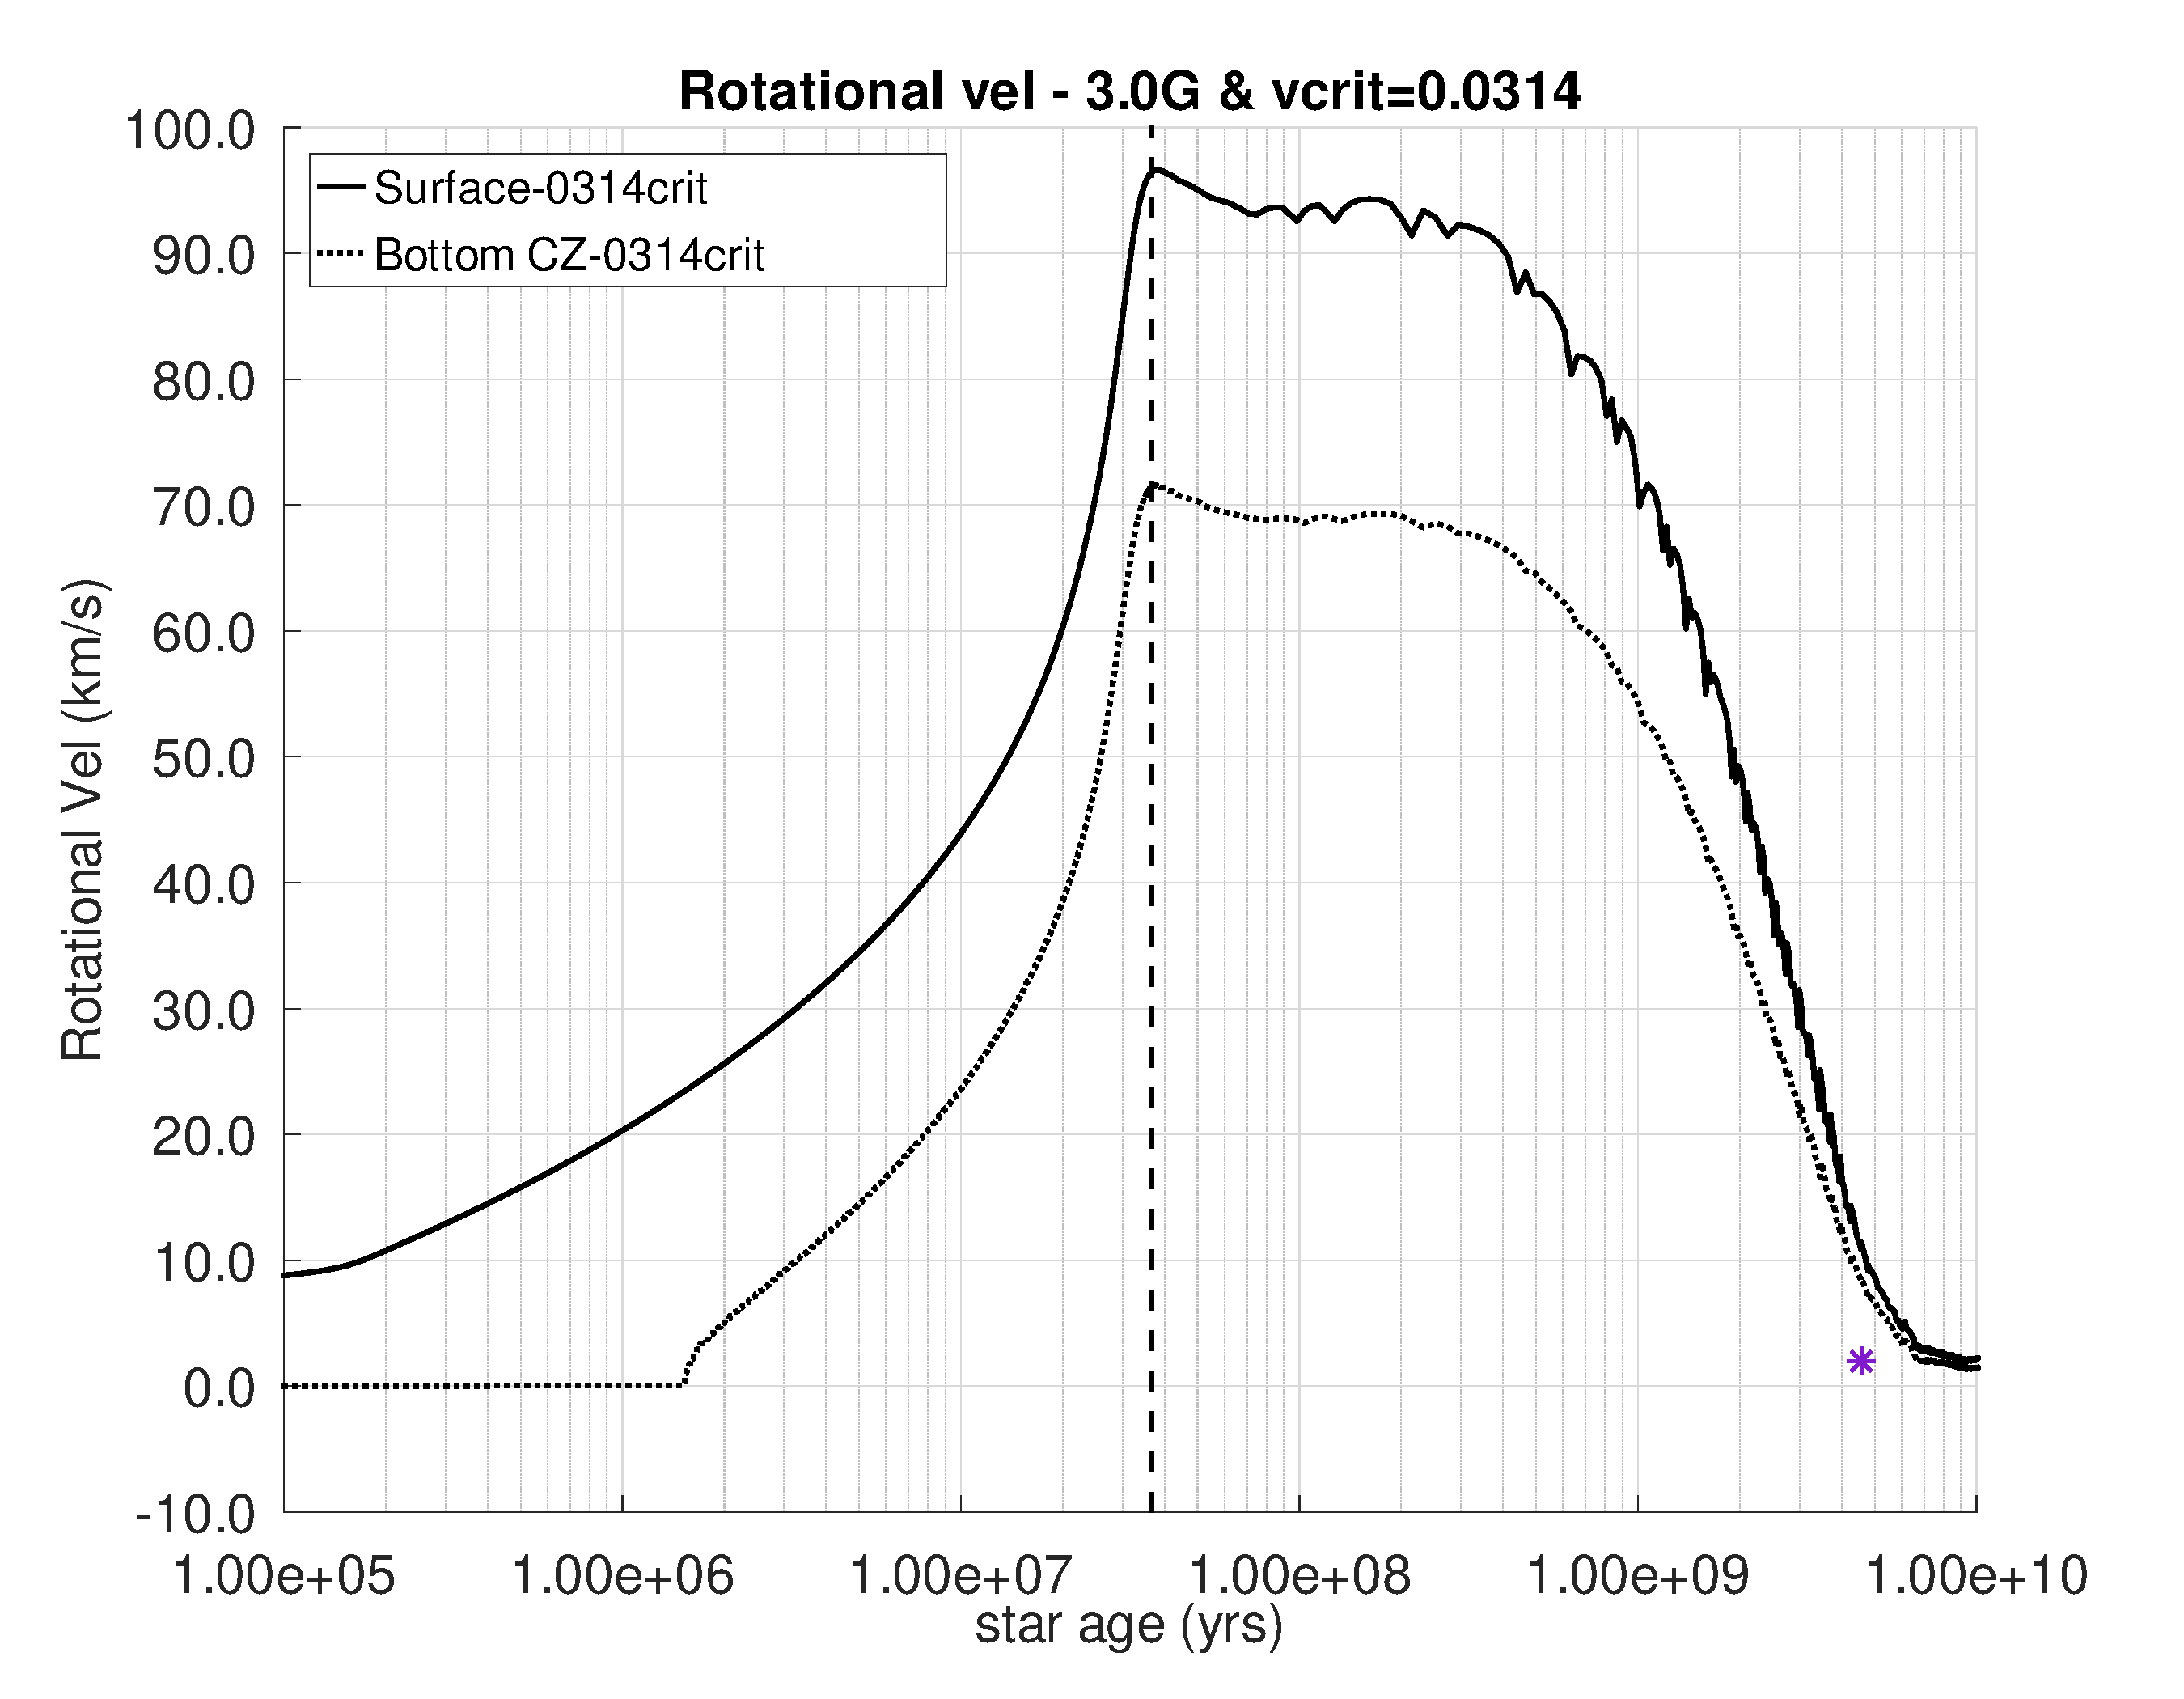
\includegraphics[width=0.7\textwidth]{img/paper1/rot_vel_3_0g_0314vc.pdf}
	\caption{La evolución de la velocidad de rotación de la superficie, en función del tiempo para un modelo de 1 $\msun$. El modelo incluye un campo magnético con una intensidad de 3G, rotación PMS con $\oomegac=0.0314$, parámetros en la Tabla \ref{tab:phy_alt_mesa} y MB. La estrella púrpura es la velocidad angular superficial para el Sol actual \cite{Gill2012}. La línea vertical discontinua hace referencia a la ZAMS.}
	\label{fig:rot_vel_var_vel_mlt_3_0g}
\end{figure}

\section{Conclusiones} \label{sec_conclusions_i}
Hemos demostrado, a través de los diferentes modelos estelares simulados, que los efectos inducidos por la combinación de ambos mecanismos de rotación y frenado magnético ofrecen una forma plausible de reconciliar los datos observacionales con los modelos teóricos. Esto último es de gran importancia tanto para el transporte de AM como para el transporte de elementos químicos. También somos muy conscientes de que aún estamos lejos de comprender los mecanismos físicos exactos que gobiernan estos procesos, por lo que es necesario seguir profundizando en estas áreas de estudio. En particular, el estudio de la evolución de los campos magnéticos durante la PMS y la MS, y su impacto en la AML. \par

Se realizarán futuras y mejoradas implementaciones de nuestra rutina para estudiar los resultados sobre las huellas, la composición superficial del Li, la rotación, etc. Es probable que en un modelo estelar en rotación simulado con MB desde el principio, la rotación diferencial sea muy reducida y, por tanto, las abundancias de Li observadas en estrellas jóvenes podrían explicarse adecuadamente. Proponemos que este resultado podría alcanzarse mediante una ley de interdependencia entre $\Omega$ y $B$. Así, durante el PMS, cuando la estrella rota más rápido, el efecto MB es más eficiente. En cambio, durante el MS, cuando el arranque se ralentiza, el MB será menos intenso. Este enfoque establecería un mecanismo de autorregulación sobre la velocidad angular de la estrella que acabaría influyendo directamente en la evolución del Li. Es igualmente importante comprender mejor el papel general de la pérdida de masa en AML y sobre todo en estrellas más frías y de baja masa. Hoy en día es un reto determinar la velocidad terminal del viento estelar para este tipo de estrellas que juega un papel clave en la AML.\par

Subrayamos también que nuestros modelos no coincidieron al mismo tiempo con la abundancia de Li solar observada y $\Omega$. Por lo tanto, no podemos asegurar que hayamos modelado correctamente la historia rotacional del Sol. En vista de estas deficiencias de nuestros modelos, debemos analizar los resultados obtenidos con cautela y no sacar conclusiones prematuras. También hemos mostrado cómo una parametrización MLT alternativa podría producir resultados acordes con las observaciones. En el transcurso de este trabajo se han apoyado las siguientes conclusiones:
\begin{enumerate}
	\item La inclusión del campo magnético conduce a modelos más fríos y a un menor agotamiento de Li en la EM.
	\item Una combinación de rotación durante la PMS y efecto MB durante la MS produce un comportamiento diferente y potencialmente más prometedor que los producidos por los modelos estándar. Así, nuestro enfoque apunta a reproducir el A(Li) observado y la velocidad de rotación solar al mismo tiempo.
	\item $\teff$ de las trayectorias evolutivas estándar representan límites superiores, ya que estos modelos no tienen en cuenta el efecto de frenado magnético ni la rotación.
	\item La extensión de la zona convectiva disminuye cuando aumenta la intensidad del campo magnético.
	\item El MB durante la PMS y/o el ajuste de los parámetros libres de exceso de MLT y $\amlt$ parece ser también necesario para explicar las abundancias de Li en cúmulos jóvenes.
\end{enumerate}

\endinput
%--------------------------------------------------------------------
% FIN DEL CAPÍTULO. 
%--------------------------------------------------------------------


\cleardoublepage
\part{Rotación y campos magnéticos de intensidad variable}
% !TeX root = ../libro.tex
% !TeX encoding = utf8

\chapter{Rotación y campos magnéticos de intensidad variable}\label{ch:sexto-capitulo}

\section{Introducción}
--ELABORAR LA INTRODUCCIÓN. REVISAR PAPER2--
Suponer que la intensidad del campo magnético de una estrella permanece constante a lo largo de su evolución es una simplificación necesaria en algunos escenarios, pero no se corresponde con las observaciones (INDICAR LAS REFERENCIAS). \par

--EXPLICAR POR QUÉ OPTAMOS POR LA INTENSIDAD VARIABLE
La segunda línea de trabajo se encaminó a extender MESA para que soportara la influencia de campos magnéticos y $\amlt$ variable en la evolución de su estrella anfitriona.
Adicionalmente a lo de la parte 1
\begin{itemize}
	\item Presencia de campo magnético de intensidad variable
	\item Evolución temporal de $\amlt$
\end{itemize}
\section{Efectos del frenado magnético - Parte II}

\subsection{Formalismo de frenado magnético de intesidad variable} 
De acuerdo a \cite{Gallet2013} la intensidad del campo magnético debería variar a lo largo de la vida de la estrella en lugar de permanecer fija durante toda su evolución. Para ello nos basamos en un formalismo que nos permite calcular una intensidad de campo magnético variable. 

\subsubsection{Frenado magnético según Gallet \& Bouvier (2013)}
Este modelo adopta una prescripción de tipo dinamo que permite establecer una relación entre $\Omega$ , $\teff$, y la intensidad del campo magnético ($B$), así como con la tasa de pérdida de masa ($\mwind$) causada por el viento estelar. Comenzaremos enumerando los aspectos más relevantes y las suposiciones realizadas en la modelización de la evolución de la intensidad del campo magnético.\par 

Un parámetro relevante para caracterizar la influencia de un campo magnético dado en el viento estelar es $\Omega$. Suponiendo que el campo magnético es generado por una dinamo, su fuerza es proporcional a alguna potencia de $\Omega$,

\begin{equation}
	f_*B_* \propto \Omega_*^b \label{eq:mf_strenght}
\end{equation}

donde $f_*$ es el factor de llenado, es decir, la fracción de la superficie estelar que está magnetizada, $B_*$ es la fuerza del campo magnético, $\Omega_*$ es la velocidad angular de la estrella en la superficie estelar, y $b$ es el exponente de la dinamo \citep{Gallet2013}. El producto de $f_*$ por $B_*$ nos permitirá obtener la intensidad del campo magnético. \par

Según este enfoque, la intensidad del campo magnético variará proporcionalmente a la temperatura efectiva ($\teff$) de la estrella de la siguiente manera: 
\begin{ceqn}
	\begin{equation}
		B_* \approx 1.13 \Beq \label{eq:mf_bstar}
	\end{equation}
\end{ceqn}

donde $B_*$ es proporcional a la intensidad del campo magnético de equipartición, quedando $\Beq$ definido como 

\begin{equation}
	\Beq = \sqrt{8\pi P_*} = \sqrt{\frac{8\pi\rho_* \boltzmann \teff}{\mu\massH}}\label{eq:mf_beq}    
\end{equation}

donde $P_*$ es la presión del gas fotosférico, $\rho_*$ es la densidad fotosférica, $\boltzmann$ es la constante de Boltzmann, $\massH$ es la masa de un átomo de hidrógeno, y $\mu$ el peso atómico medio \citep{Cranmer2011}. \par

Como se indica en \cite{Cranmer2011} $\mu$ puede estimarse utilizando las ecuaciones de estado del plasma OPAL \footnote{\url{https://opalopacity.llnl.gov/EOS_2005/}},

\begin{equation}
	\mu \approx \frac{7}{4} + \frac{1}{2} \; \textrm{tanh}\Bigg(\frac{3500-\teff}{600}\;\Bigg) \label{eq:mf_atom_weight}
\end{equation}

Finalmente, estamos en condiciones de calcular $\Beq$ y $B_*$.\par

Por otro lado, \cite{Cranmer2011} descubrió que la intensidad del campo magnético está influida principalmente por $f_*$ y no por el periodo de rotación de la estrella. Es decir, las variaciones en la velocidad angular de la estrella no alteran significativamente la intensidad de su campo magnético. Además, $f_*$ depende en gran medida del número de Rossby ($\rossby$). Para calcular $\rossby$ de una estrella determinada, es necesario conocer el tiempo de vuelta ($\turnover$),

\begin{equation}
	\rossby = \frac{\prot}{\turnover} \label{eq:mf_rossby}
\end{equation}
\begin{equation}
	\turnover = 314.24\;exp\left[-\Bigg(\frac{\teff}{1952.5}\Bigg)-\Bigg(\frac{\teff}{6250}\Bigg)^{18} \;\right]+0.002 \label{eq:mf_turnover}
\end{equation}

\cite{Cranmer2011} proporciona dos ajustes diferentes para $f_*$ que definen respectivamente los límites superior e inferior para la intensidad media del campo magnético superficial ($f_*B_*$),

\begin{align}
	\fmin &= \frac{0.5}{(1+(x/0.16)^{2.6})^{1.3}} \label{eq:fmin}\\
	\fmax &= \frac{1}{1+(x/0.31)^{2.5}} \label{eq:fmax}
\end{align}

donde x = $\rossby$/$\rossbysun$, y $\rossbysun$ = 1.96. \par

Por último, podemos calcular el factor de llenado de una estrella aplicando el ajuste realizado por \cite{Gallet2013} que reproduce más fielmente el factor de llenado medio del Sol actual ($\fsun$ = [0.001-0.01], ver \citep{Cranmer2011}),


\begin{figure}
	\centering
	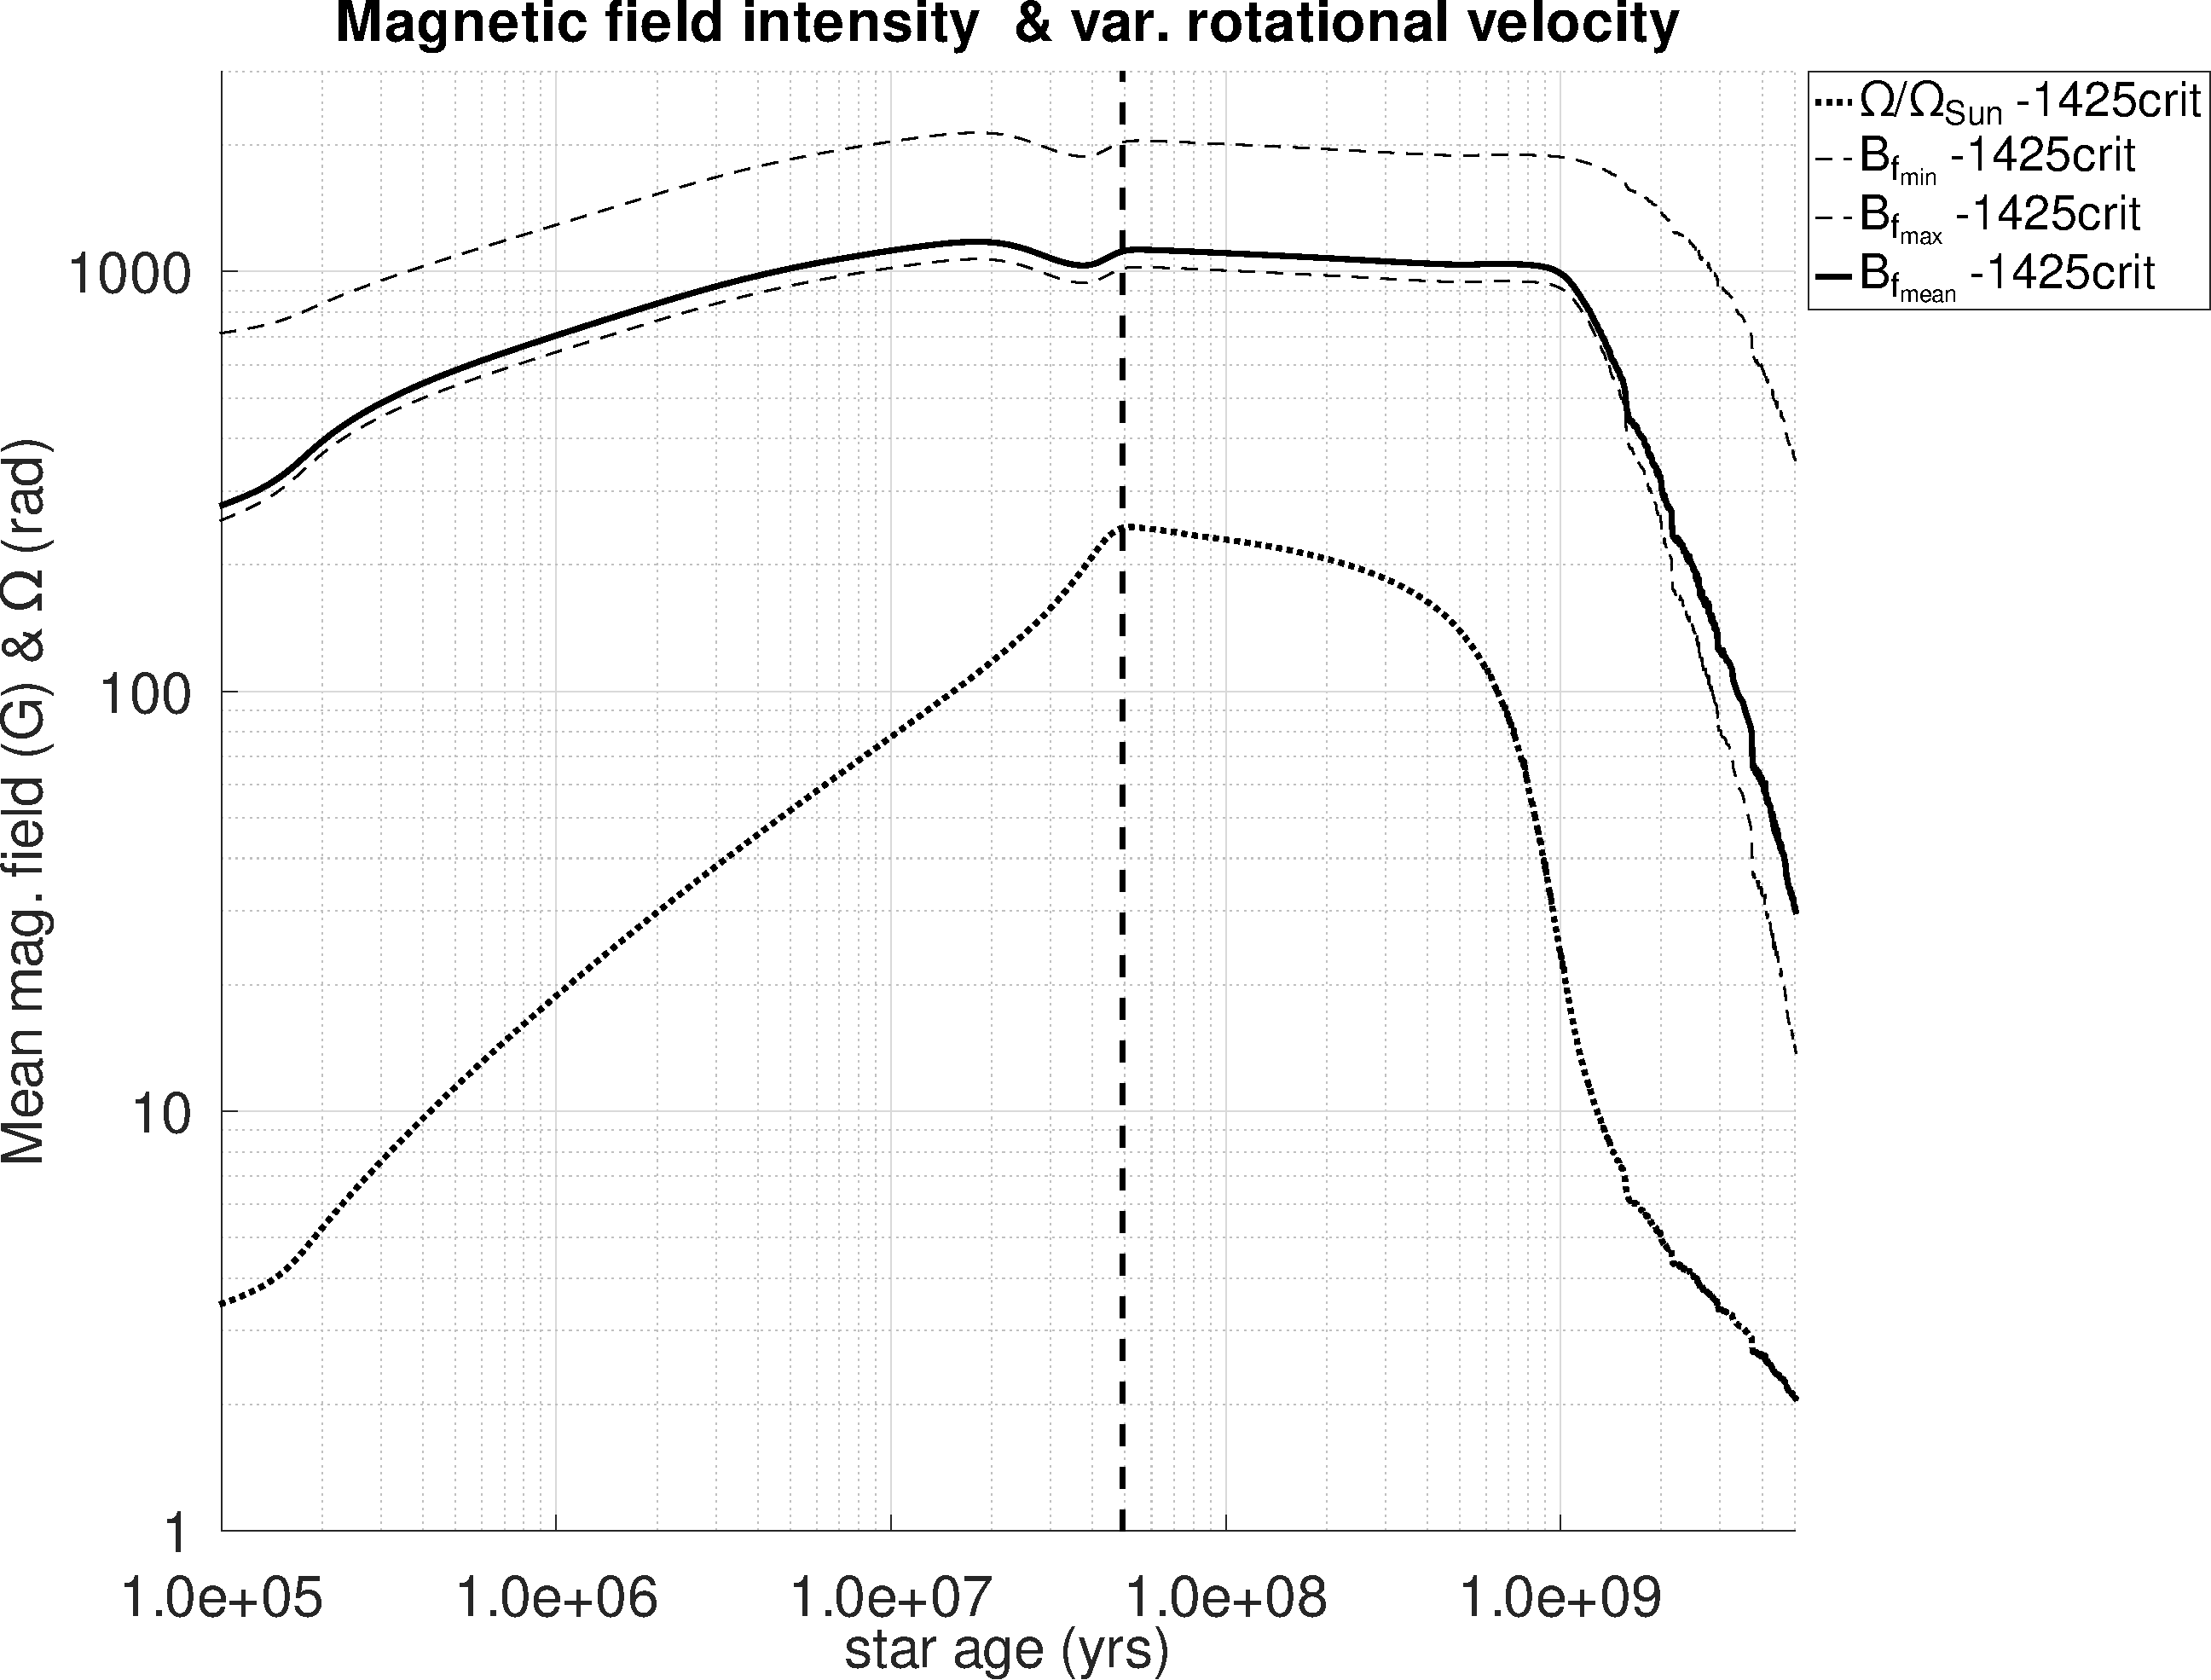
\includegraphics[width=0.5\textwidth]{img/paper2/mag_field_limits_var_vel_g3.pdf}
	\caption{La evolución de la intensidad del campo magnético y sus límites superior e inferior, en función del tiempo y $\oomegac$ para varios modelos de 1 $\msun$. El modelo incluye rotación PMS con $\oomegac$ = 0.1425. Las líneas continuas representan la intensidad del campo magnético, mientras que las líneas discontinuas representan la evolución angular de la estrella. La línea vertical discontinua hace referencia a la ZAMS.}
	\label{fig:mag_field_limits_var_vel_g3}
\end{figure}

Con este formalismo podemos calcular el campo magnético medio como una función dependiente del tiempo, de $\rho$, $\teff$, y $\Omega$. Los valores temporales de estas tres variables se obtendrán a partir de las distintas simulaciones realizadas con ayuda de MESA. \par


--QUIZAS SACARLO A UNA SECCIÓN PROPIA DE AML --
Una vez que hemos caracterizado cómo evoluciona la intensidad del campo magnético, necesitamos modelar cómo se produce la pérdida de momento angular. A medida que la estrella se contrae durante la fase de PMS hacia el comienzo de la ZAMS, su velocidad angular aumenta, lo que conduce a un aumento gradual del campo magnético medio. En nuestro análisis, observamos intensidades máximas de hasta $1.0,\mathrm{kG}$, como se muestra en la figura \ref{fig:mag_field_limits_var_vel_g3}. A continuación, entra en una fase de saturación (aunque con una tendencia descendente) hasta $1.0$ Ga, y finalmente disminuye bruscamente como resultado de la menor velocidad angular de la estrella. En el formalismo anterior utilizamos un modelo aplicable a campos magnéticos de intensidad no variable y de baja intensidad que oscilan entre unos pocos Gauss ($1.0,\mathrm{G} \leq B \leq 10.0,\mathrm{G}$). Las intensidades significativamente mayores requeridas en el presente formalismo hacen inadecuado el modelo empleado anteriormente.\par


Comencemos por enumerar los aspectos más relevantes y las suposiciones realizadas en la modelización de la evolución de la rotación, el frenado magnético y el momento angular. Si suponemos un flujo de salida esférico, el par aplicado por un viento estelar $\torquewind$ acoplado magnéticamente viene dictado por,

\begin{equation}
	\torquewind \propto \Omega_* \; \mwind \; \ralfven^{2} \label{eq:mb_torque}
\end{equation}

donde $\mwind$ es la tasa de pérdida de masa, y $\ralfven$ el valor medio del radio de Alfvén. \par

Las estrellas con masas iniciales similares, pero con diferentes ratios de pérdida de masa ($\Dot{M}$), acabarán evolucionando de forma muy diferente. Las partículas ionizadas transportadas por el viento solar no sólo contribuyen a la pérdida de masa, sino también a la pérdida de energía cinética que se deposita en el medio interestelar. Dada una estrella con un viento esféricamente simétrico, $\mwind$ se caracteriza por la siguiente expresión:

\begin{ceqn}
	\begin{equation}
		\mwind = 4\pi r^2\rho\nu \label{eq:mass_loss}
	\end{equation}
\end{ceqn}

donde $r$ es el radio estelar, $\rho$ la densidad de masa, y $\nu$ la velocidad del viento estelar.

--BLOQUE REPETIDO. HACER REFERENCIA A LA SECCIÓN ANTERIOR, INDICANDO QUE A DIFERENCIA DE ELLA, AQUÍ UTILIZAMOS R-ALVEN--
Se ha observado que las estrellas de masa intermedia fuertemente magnéticas suelen tener tasas de rotación mucho más lentas que otras estrellas de su población parental \cite{Mathys2006}. En esas estrellas, los campos magnéticos interactúan con la pérdida de masa, donde el radio Alfv'{e}n juega un papel importante. $\ralfven$ se define como el punto en el que la densidad de energía del campo magnético y la densidad de energía cinética están equilibradas. En caso de que $\ralfven$ sea mayor que el radio estelar, entonces el flujo del viento tendrá que seguir el campo magnético. Como consecuencia, el material abandona la superficie estelar con una mayor AM específica, ya que el radio de co-rotación ha aumentado y corresponde aproximadamente a $\ralfven$ que puede expresarse como \cite{Matt2012}

\begin{equation}
	\ralfven = K_1\left[\frac{\Bp^{2}\;R_*^{2}}{\mwind\;\sqrt{K_2^2\vesc^2 + \Omega_*^2R_*^{2}}\ }\right]^{m}R_*  \label{eq:mb_ralfven}
\end{equation}

donde $\Bp$ es la intensidad del campo magnético en la superficie estelar, $\vesc$ es la velocidad de escape, $m = 0.1675$, $K_1 = 1.30$ y $K_2 = 0.0506$ \citep{Gallet2013}.

\begin{align}
	\Bp &= f_*B_* \label{eq:bp}\\
	\vesc &= \sqrt{\frac{2\,G\,\mstar}{\rstar}} \label{eq:vesc}
\end{align}

Por último, tenemos que el AML puede calcularse del siguiente modo:

\begin{equation}
	\Dot{J} = \Omega_* \; \mwind \; \ralfven^{2} \label{eq:j_dot}
\end{equation}

donde $\mwind$ es la tasa de pérdida de masa. Esta expresión se implementa en MESA a partir de los valores expuestos directamente durante las simulaciones.

--HASTA AQUÍ--

\section{Efectos de la longitud de mezcla}
La teoría de la longitud de mezcla (Mixing Length Theory, MLT) introducida por \citet{BohmVit58} ha sido comúnmente adoptada para modelar la convección estelar en códigos de evolución estelar, incluyendo MESA. El parámetro libre más importante en esta teoría es la longitud de mezcla $l$ que se define como:

\begin{equation}
	l = \alpha H_p\label{eq:mixlength}
\end{equation}

donde $H_p$ es la altura de la escala de presión, y $\alpha$ un parámetro libre que se determina de antemano y se mantiene fijo durante las simulaciones de evolución estelar. \par

La influencia de los parámetros libres, relativamente arbitrarios, asociados a MLT condiciona significativamente la evolución de la abundancia de Li. Además, no existen argumentos sólidos que sugieran que el parámetro de longitud de mezcla sea el mismo en todas las estrellas y en todas las fases evolutivas \cite{Pasetto2014}. En la Sección \ref{sec:alt_mlt} mostramos cómo una parametrización alternativa de la longitud de mezcla (ML) podría producir resultados en línea con las observaciones. El ajuste del overshooting de ML y del parámetro libre $\amlt$ parece ser necesario para explicar las abundancias de litio en los OC's.\par

De manera similar a la intensidad del campo magnético, un formalismo que nos permita evolucionar a lo largo del tiempo el valor de $\amlt$ en función de determinados parámetros de la estrella, es un planteamiento razonable a la hora de eliminar una restricción relativamente arbitraria impuesta en nuestros modelos.

\subsection{MLT $\alpha$ variable según Sonoi et al. (2019)}
En \cite{Sonoi2018}, los autores introdujeron una forma de calibrar $\amlt$ para estrellas de tipo solar en la que su valor directamente proporcional a la $\gsurf$, e inversamente proporcional a la $\teff$. --CREAN UN SIMPLE EXCEL MOSTRANDO ESTO-- Calibraron diferentes valores de $\amlt$ para varios modelos 3D simulados usando el código CO$^5$BOLD \citep{Freytag2011} y los transfirieron a modelos 1D desarrollados por \cite{Ludwig1998}. La parametrización que obtuvieron fue: 

\begin{equation}
	f(x,y) = a_0 + (a_1 + (a_3 + a_5x +a_6y)x + a_4y)x + a_2y\label{eq:alpha_ml}
\end{equation}

donde

\begin{align}
	x &= \frac{\teff-5777}{1000} \label{eq:eq:alpha_x}\\
	y &= \gsurf-4.44 \label{eq:eq:alpha_y}
\end{align}

y $a_i$ son los coeficientes resultantes de la función de ajuste \ref{eq:alpha_ml} a los valores $\alpha$ calibrados para el modelo de convección MLT \citep{Sonoi2018}: $a_0=1.790295$, $a_1=-0.14954$, $a_2=0.069574$, $a_3=-0.00829$, $a_4=0.013165$, $a_5=0.080333$, $a_6=-0.03306$. \par
--COMENTAR MÁS EN DETALLE CÓMO, POR EJEMPLO, SE HACE VARIAR EN MESA. TAMBIÉN ALGO MÁS DEL FORMALISMO--



\section{Extendiendo MESA - Parte III}
\subsection{Rutina de frenado magnético de intensidad variable} \label{sec:mb_var_b}
En la Sección \ref{sec:mb_cte_b} comentamos los detalles de como MESA conserva el AM entre las diferentes celdas $k$ y les asigna un valor de AM $J_k$. Este mecanismo sigue siendo el mismo para esta nueva rutina. En este nuevo escenario la diferencia radica en la nueva rutina de MB (ver Listado \ref{lst:jdot_gb}), concretamente en la implementación de la misma según el nuevo formalismo que hemos introducido para campos magnéticos de intensidad variable, y especialmente en la rutina que calcula la intensidad del campo magnético, devolviendo (potencialmente) un valor diferente a cada paso de la simulación (ver Listado \ref{lst:jdot_mf_intensity}).\par

\begin{lstlisting}[language=Fortran, float, caption={Rutina de par de torsión para un campo magnético de intensidad variable.}, label={lst:jdot_gb}]
  real function calculate_jdot_rate_gb(s, bf_star) result(new_j_dot)
	use const_def
	type (star_info), pointer, intent(in) :: s
	real(dp), intent(in) :: bf_star
	real(dp), parameter :: k1 = 1.30
	real(dp), parameter :: k2 = 0.0506
	real(dp), parameter :: m = 0.1675
	real(dp), parameter :: omega_sun = 2.87d-6
	real(dp) :: r_st, m_st, omega_surf, j_dot
	real(dp) :: v_esc, m_dot, alfven_r, alfven_r_num, alfven_r_den
	
	!Star data
	r_st = s% r(1)
	m_st = s% m(1)
	omega_surf = s% omega(1)
	m_dot = abs(s% mstar_dot) !This in g/s
	
	v_esc = (2 * standard_cgrav * m_st / r_st)**0.5
	
	alfven_r_num = bf_star**2 * r_st**2
	alfven_r_den = m_dot*((k2**2 * v_esc**2)+(omega_surf**2 * r_st**2))**0.5
	alfven_r = k1 * (alfven_r_num / alfven_r_den)**m * r_st
	
	j_dot = omega_surf * m_dot * alfven_r**2
	
	new_j_dot = -j_dot
  end function	
\end{lstlisting}

\subsection{Rutina de cálculo de intensidad de campo magnético}
La incorporación del formalismo para calcular una intensidad de campo magnético variable representa una mejora sustancial al modelo presentado en el capítulo \ref{ch:tercer-capitulo}. Esta intensidad es funcionalmente dependiente del tiempo, de $\rho$, $\teff$, y $\Omega$, valores que podemos obtener directamente de MESA.\par

\begin{lstlisting}[language=Fortran, float, caption={Rutina de cálculo de intensidad de campo magnético.}, label={lst:jdot_mf_intensity}]
  real function calculate_mag_field_intensity_gb(s) result(new_b)
	use const_def
	type (star_info), pointer, intent(in) :: s
	
	! rossby_sun = 1.96, Eq 9 [1]
	real(dp) :: r_st, rossby_sun = 1.96, rossby, rossby_norm, m_hydrogen
	real(dp) :: p_rot, p_rot_sun = 25.38 !Carrington solar  rotation
	real(dp) :: tau_c_sun, tau_c, f_star, f_min, f_max, b_star
	real(dp) :: bf_min, bf_max, bf_star, b_equi, mu_avg
	real(dp) :: p_gas_photo, p_photo, p_rad_photo, p_photo2
	
	!tau_c -> convective turnover time (d)
	!exp ->  natural exponential function
	tau_c = 314.241*exp(-s% Teff/1952.5)*exp(-(s% Teff/6250)**18) + 0.002 
	tau_c_sun = 314.241*exp(-teffsun/1952.5)*exp(-(teffsun/6250)**18) + 0.002
	
	!Star data
	r_st = s% r(1)
	p_rot = (2*pi*r_st) / (s% v_rot_avg_surf * 86400) ! day
	
	!Rossby number = p_rot / tau_c
	rossby = p_rot / tau_c
	rossby_sun = p_rot_sun / tau_c_sun
	rossby_norm = rossby / rossby_sun
	
	!magnetic filling factor fmin & fmax
	f_min = 0.5 / (1. + (rossby_norm / 0.16)**2.6)**1.3 
	f_max = 1 / (1. + (rossby_norm / 0.31)**2.5)
	f_star = 0.55 / (1. + (rossby_norm / 0.16)**2.3)**1.22
	
	!Eq 3 [2]
	!mean atomic weight
	mu_avg = 1.75 + 0.5 * tanh((3500. - s% Teff) / 600.)
	!photospheric pressure 
	m_hydrogen = mp !proton mass       
	p_photo = s%rho(s% photosphere_cell_k)*boltzm*s% Teff/(mu_avg*m_hydrogen)
	!Equipartition magnetic filed strength
	b_equi = sqrt(8.* pi * p_photo)
	
	!Eq 7 [1], magnetic field strength b_star is proportional to the
	!equipartition magnetic field strength b_equi
	b_star = 1.13 * b_equi
	bf_min = f_min * b_star
	bf_max = f_max * b_star
	bf_star = f_star * b_star
	
	!return the min value, as it does the paper
	new_b = bf_star
  end function	
\end{lstlisting}

\subsection{Rutina de $\amlt$ variable}
Adicionalmente, y en línea con el objetivo de reducir el número de parámetros fijos, hemos procedido a calcular, para cada paso temporal de la simulación de MESA, un valor de $\amlt$, eliminando así la necesidad de prefijar su valor para toda la simulación.\par  

\begin{lstlisting}[language=Fortran, float, caption={Rutina de $\amlt$ variable.}, label={lst:var_amlt}]
  real function calculate_alpha(s) result(new_alpha)
	type (star_info), pointer, intent(in) :: s
	
	!Parameters taken from Table 2 - MTL(BV) Eddington
	
	real(dp) :: a0 = 1.790295, a1 = -0.149542, a2 = 0.069574, a3 = -0.008292
	real(dp) :: a4 = 0.013165, a5 = 0.080333, a6 = -0.033066
	real(dp) :: x, y
	
	!f(x, y) = a0 + (a1 + (a3 + a5x + a6y)x + a4y)x + a2y
	!where x = (Teff-5777)/1000 and y = log g-4.44
	!Namely, x and y represent deviation from the solar effective 
	!temperature and surface gravity, respectively.
	x = (s% Teff - 5777) / 1000
	y = s% log_surface_gravity - 4.44
	
	new_alpha = a0 + (a1 + (a3 + a5*x + a6*y)*x + a4*y)*x + a2*y
	s% x_ctrl(47) = new_alpha
  end function
	
\end{lstlisting}

MESA no proporciona un \textit{hook} particular para modificar la rutina por defecto que trae el simulador. Para poder hacer evolucionar el valor de $\amlt$ recurrimos a incorporar nuestra rutina en la que MESA ejecuta al final de cada paso de simulación. De este modo conseguimos que en la siguiente iteración, utilice el valor que hemos calculado.
\begin{lstlisting}[language=Fortran, float, caption={Rutina de MESA para ejecutar lógica adicional tras la ejecución de un paso de simulación.}, label={lst:extra_start_step}]
  integer function extras_start_step(id, id_extra)
	integer, intent(in) :: id, id_extra
	integer :: ierr
	real(dp) :: x, y, new_alpha
	type (star_info), pointer :: s
	ierr = 0
	call star_ptr(id, s, ierr)
	if (ierr /= 0) return
	extras_start_step = keep_going
	
	if (var_mlt_alpha .eqv. .true.) then
	s% mixing_length_alpha = calculate_alpha(s)
	end if
	
  end function extras_start_step
\end{lstlisting}

\endinput
%--------------------------------------------------------------------
% FIN DEL CAPÍTULO. 
%--------------------------------------------------------------------


% !TeX root = ../libro.tex
% !TeX encoding = utf8


\chapter{Resultados de frenado magnético de intensidad variable}\label{ch:septimo-capitulo}
\section{Configuración de los modelos} \label{marco_teorico_ii}

A COMENTAR
Parametrización de los modelos
Rango de valores a asignar a los parámetros libres
Ciclo de control
Para cada paso de simulación
- Obtenemos o calculamos la intensidad del campo magnético
- Calculamos la pérdida de momento angular inducida por el campo magnético
- Distribuimos la pérdida de momento angular entre las capas de la estrella
- Obtenemos o calculamos el valor de $\amlt$


\section{Modelos de evolución estelar}
Como venimos exponiendo en el capítulo anterior, con la consideración de campos magnéticos de intensidad variable ($B$) dependientes de los parámetros estelares $\Omega$ y $\teff$ llevamos nuestra línea de trabajo un paso más allá. La parametrización base utilizada es básicamente la misma que hemos utilizado al abordar los campos magnéticos de intensidad fija. La innovación fundamental radica en la introducción de una intensidad de campo magnético variable ($B$) y un parámetro $\amlt$ variable. En cuanto al tratamiento de la mezcla convectiva con sobreimpulso (overshooting), es evidente una desviación del modelo anterior; desactivamos deliberadamente esta característica en nuestro modelo actual. Esto aísla el impacto de una variable $\amlt$ en A(Li) de los efectos asociados con el sobreimpulso convectivo. En particular, la mezcla convectiva con sobreimpulso se aborda habitualmente mediante extensiones ad hoc de la Teoría de la Longitud de Mezcla (MLT), introduciendo así un parámetro libre adicional. La Tabla \ref{tab:phy_mesa_ii} enumera las similitudes y diferencias en la configuración de los modelos utilizados en \cite{Caballero2020} y en este trabajo.\par

\begin{table}
	\begin{threeparttable}
		\centering
		\begin{tabular}{ll} 
			\hline
			Parámetro & Prescripciones y valores adoptados\\
			\hline
			Abundancia Solar & $X_{\odot}=0.7154, Y_{\odot}=0.2703, Z_{\odot}=0.0142$\\
			Ecuación de estado & OPAL+SCVH+MacDonald+HELM+PC\\
			Opacidad & OPAL Tipo I para log T $\geq$ 4 \\ & Ferguson para logT $<$ 4\\
			Tasas de Reacción & JINA REACLIB\\
			Condiciones de Contorno & ATLAS12; $\tau$=100 tablas + fotoesfera\\
			Difusión & Rastreo de \isotope[1]{H}, \isotope[2]{He}, \isotope[7]{Li}, \isotope[7]{Be}\\
			Esquema de Rotación & Rotación diferencial en PMS \& MS\\ & Incluye SH\tnote{1}  , ES\tnote{2}  , GSF\tnote{3}  , SSI\tnote{4}  , DSI\tnote{5}\\
			Termohalina & $\alpha_{\textrm{th}}=666$\\
			\textbf{Convección} & $\alpha_{\textrm{MLT}}$ variable dependiente de $\teff$\\ & \& $\gsurf$ + Ledoux\\
			Semiconvección & $\alpha_{\textrm{sc}}=0.1$\\
			\textbf{Sobreimpulso} & $f_{\textrm{ov,core}}=0.0$, \& $f_{\textrm{ov,sh}}=0.0$\\
			\textbf{Campo Magnético} & B(G) variable, dependiente de $\rho$, $\teff$ \&  $\Omega$\\
			Pérdida de Masa & $\Dot{M}_{\textrm{max}} = 10^{-3} \: \msun \: yr^{-1}$\\
			Périda de Momento Angular & $\Dot{J} = \Omega_* \; \mwind \; \ralfven^2$\\
			\hline
		\end{tabular}
		\begin{tablenotes}\footnotesize
			\item (1) Solberg-Hoiland, (2) Eddington–Sweet
			\item (3) Goldreich–Schubert–Fricke, (4) Secular Shear Instability
			\item (5) Dynamical Shear Instability
		\end{tablenotes}
	\end{threeparttable}
	\caption{Resumen de la física adoptada en MESA \cite{Choi2016,Caballero2020}[basado en][]. Resaltados en negrita los parámetros con diferente configuración de los trabajos referenciados.}
	\label{tab:phy_mesa_ii}
	
\end{table}


Los modelos incluyen rotación desde el PMS. Hemos calculado la evolución de modelos estelares de $1\,\msun$ en metalicidad inicial solar con $\omegaini = \oomegac$ que varía entre $0.12$ y $0.1425$. A continuación, los resultados se comparan con las edades estelares de estrellas en OC recogidas por la misión Gaia y GES y referenciadas en la Tabla \ref{tab:oc_reduced_list}.\par

\subsection{Evolución del Li con MB de intensidad variable}
Existen evidencias que abogan por una fuerte relación establecida entre la destrucción de Li y la rotación estelar, de forma que cuanto mayor es la velocidad angular, mayor es la destrucción de Li (ver \cite{Bouvier2018, Caballero2020}). El efecto del MB en la evolución temporal de A(Li) viene dado por su capacidad para eliminar AM de la estrella, y por tanto influir en su velocidad de rotación, haciendo que la estrella rote más lentamente y destruya menos Li.\par

En la figura \ref{fig:li_var_vel_var_g_3} se muestra la evolución temporal de la abundancia superficial de Li para varios modelos de 1 $\msun$. Estos modelos se inicializaron con diferentes velocidades de rotación y tuvieron en cuenta los efectos del MB causado por un campo magnético variable. Si lo comparamos con la Figura \ref{fig:li_var_vel_0g} en la que se despreciaron los efectos del MB, observamos cómo se alteraron los perfiles de abundancia de Li a lo largo del PMS y el MS. Durante el PMS podemos describir el efecto como modesto, algo esperado y en línea con el hecho de que el AML causado por MB (ver Ec.~\ref{eq:j_dot}) depende directamente de la evolución de $\Omega$ y de la tasa de pérdida de masa. Si tenemos en cuenta que para las estrellas de tipo solar los modelos predicen una tasa de pérdida de masa total modesta, ese valor es incluso mucho menor en esta fase. Es en la fase de aproximación a la ZAMS cuando la velocidad angular alcanza su máximo. Esto, según nuestro modelo, desempeña un papel crucial tanto en la pérdida de masa como en la intensidad del campo magnético. Cuanto mayor sea $\Omega$, mayor será $\Dot{M}$ (véase la Figura \ref{fig:mdot_var_vel_g3}), y mayor será la intensidad del campo magnético (véase la Figura \ref{fig:mag_field_var_vel_g3}). Estos efectos se combinan y conducen a una acentuación del efecto de frenado magnético. Como consecuencia, se produce una ralentización de la destrucción del Li una vez que los modelos entran en el EM. Los resultados de nuestras simulaciones para esos modelos inicializados respectivamente a $\omegaini$ = 0.14 y 0.1425 reproducen A(Li) en línea con la de la abundancia del \isotope[7]{Li} de la superficie del Sol (1,1 $\pm$ 0,1 dex). Este último da un valor de 1,133 dex, lo que representaría una desviación de aproximadamente el 3\% del valor nominal (véase la Figura \ref{fig:li_var_vel_var_g_3}).\par

\begin{figure}
	\centering
	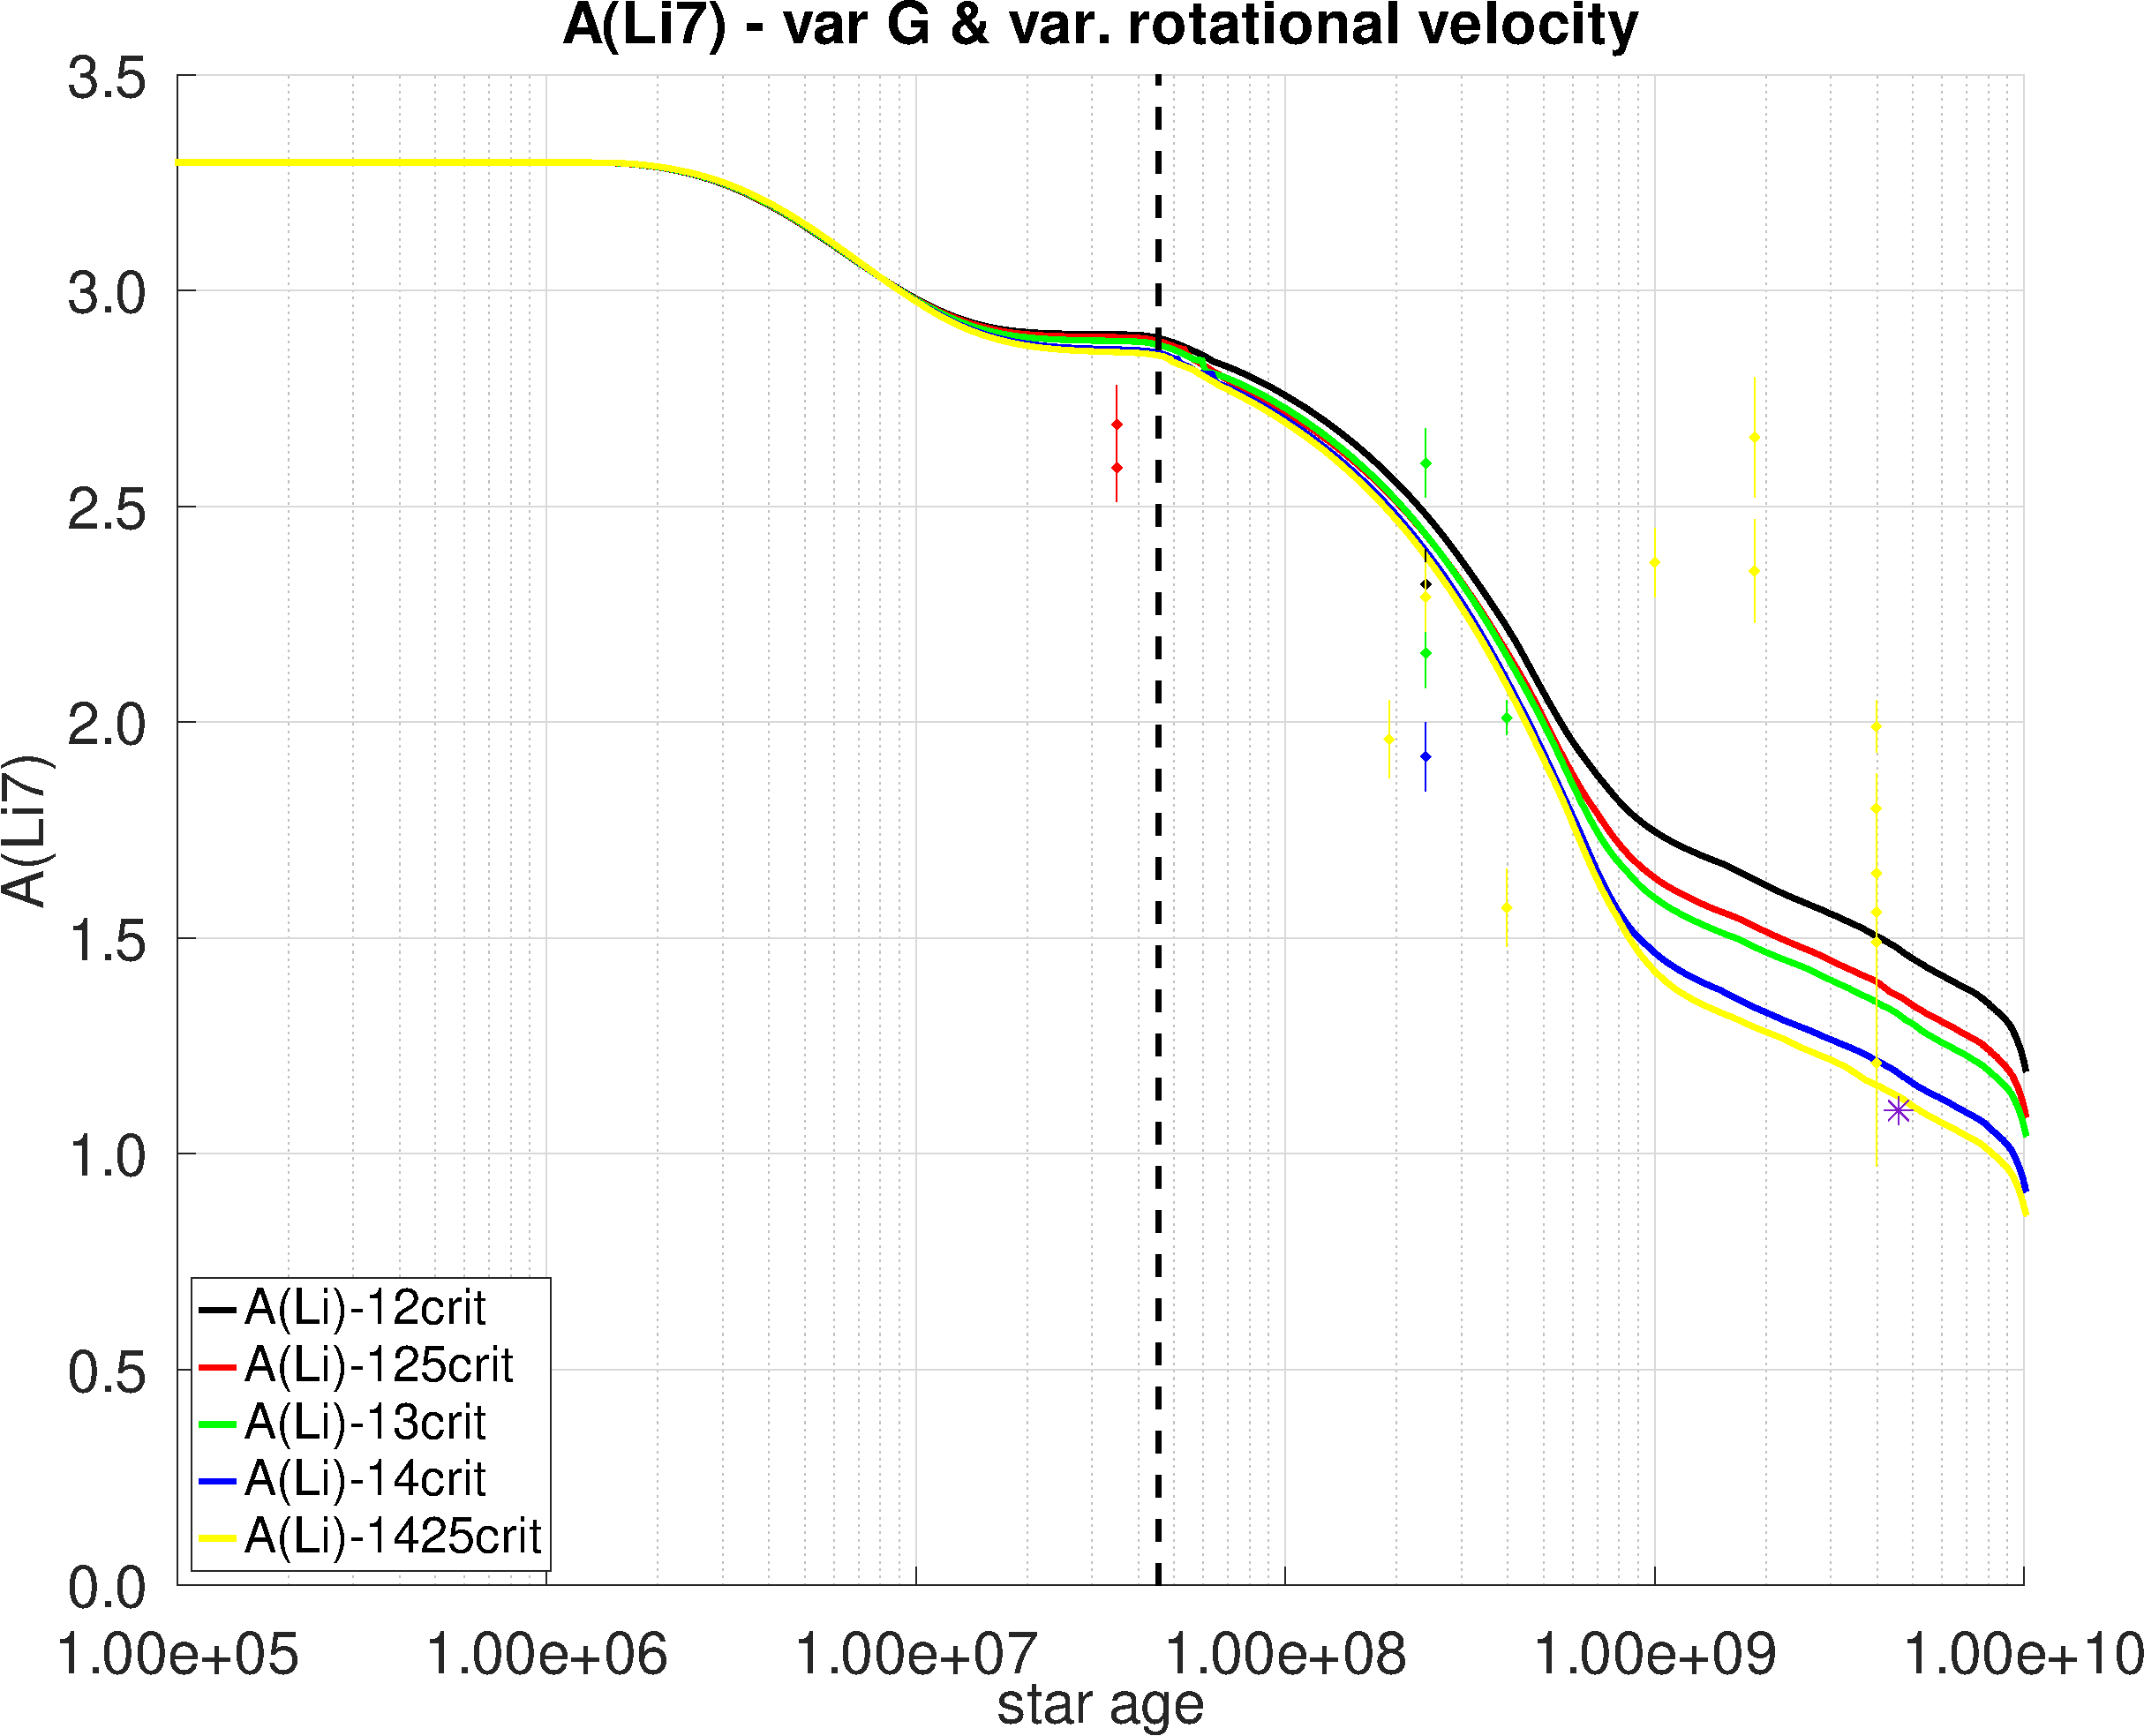
\includegraphics[width=0.7\textwidth]{img/paper2/li_var_vel_var_g_3.pdf}
	\caption{Se muestra la evolución de la abundancia relativa en superficie del \isotope[7]{Li} en comparación con el \isotope[1]{H} para varios modelos de 1 $\msun$. Éstos incluyen un campo magnético de intensidad variable, tasas de rotación iniciales que oscilan entre 0.12 y 0.1425 $\omegaini$, y MB. La estrella púrpura representa la abundancia actual de Li en la superficie del Sol \cite{Asplund2009}. Los otros puntos de color representan las abundancias superficiales de \isotope[7]{Li} para estrellas con parámetros dentro de los intervalos de selección especificados, correspondientes a la curva de evolución del mismo color. La línea vertical discontinua indica la Secuencia Principal de Edad Cero (ZAMS).}
	\label{fig:li_var_vel_var_g_3}
\end{figure}

-----------------------------------------------------------------------
----ESTA FIGURA HABRÁ QUE QUITARLA PORQUE SE INCLUYE YA ANTERIORMENTE--
-----------------------------------------------------------------------

\begin{figure}
	\centering
	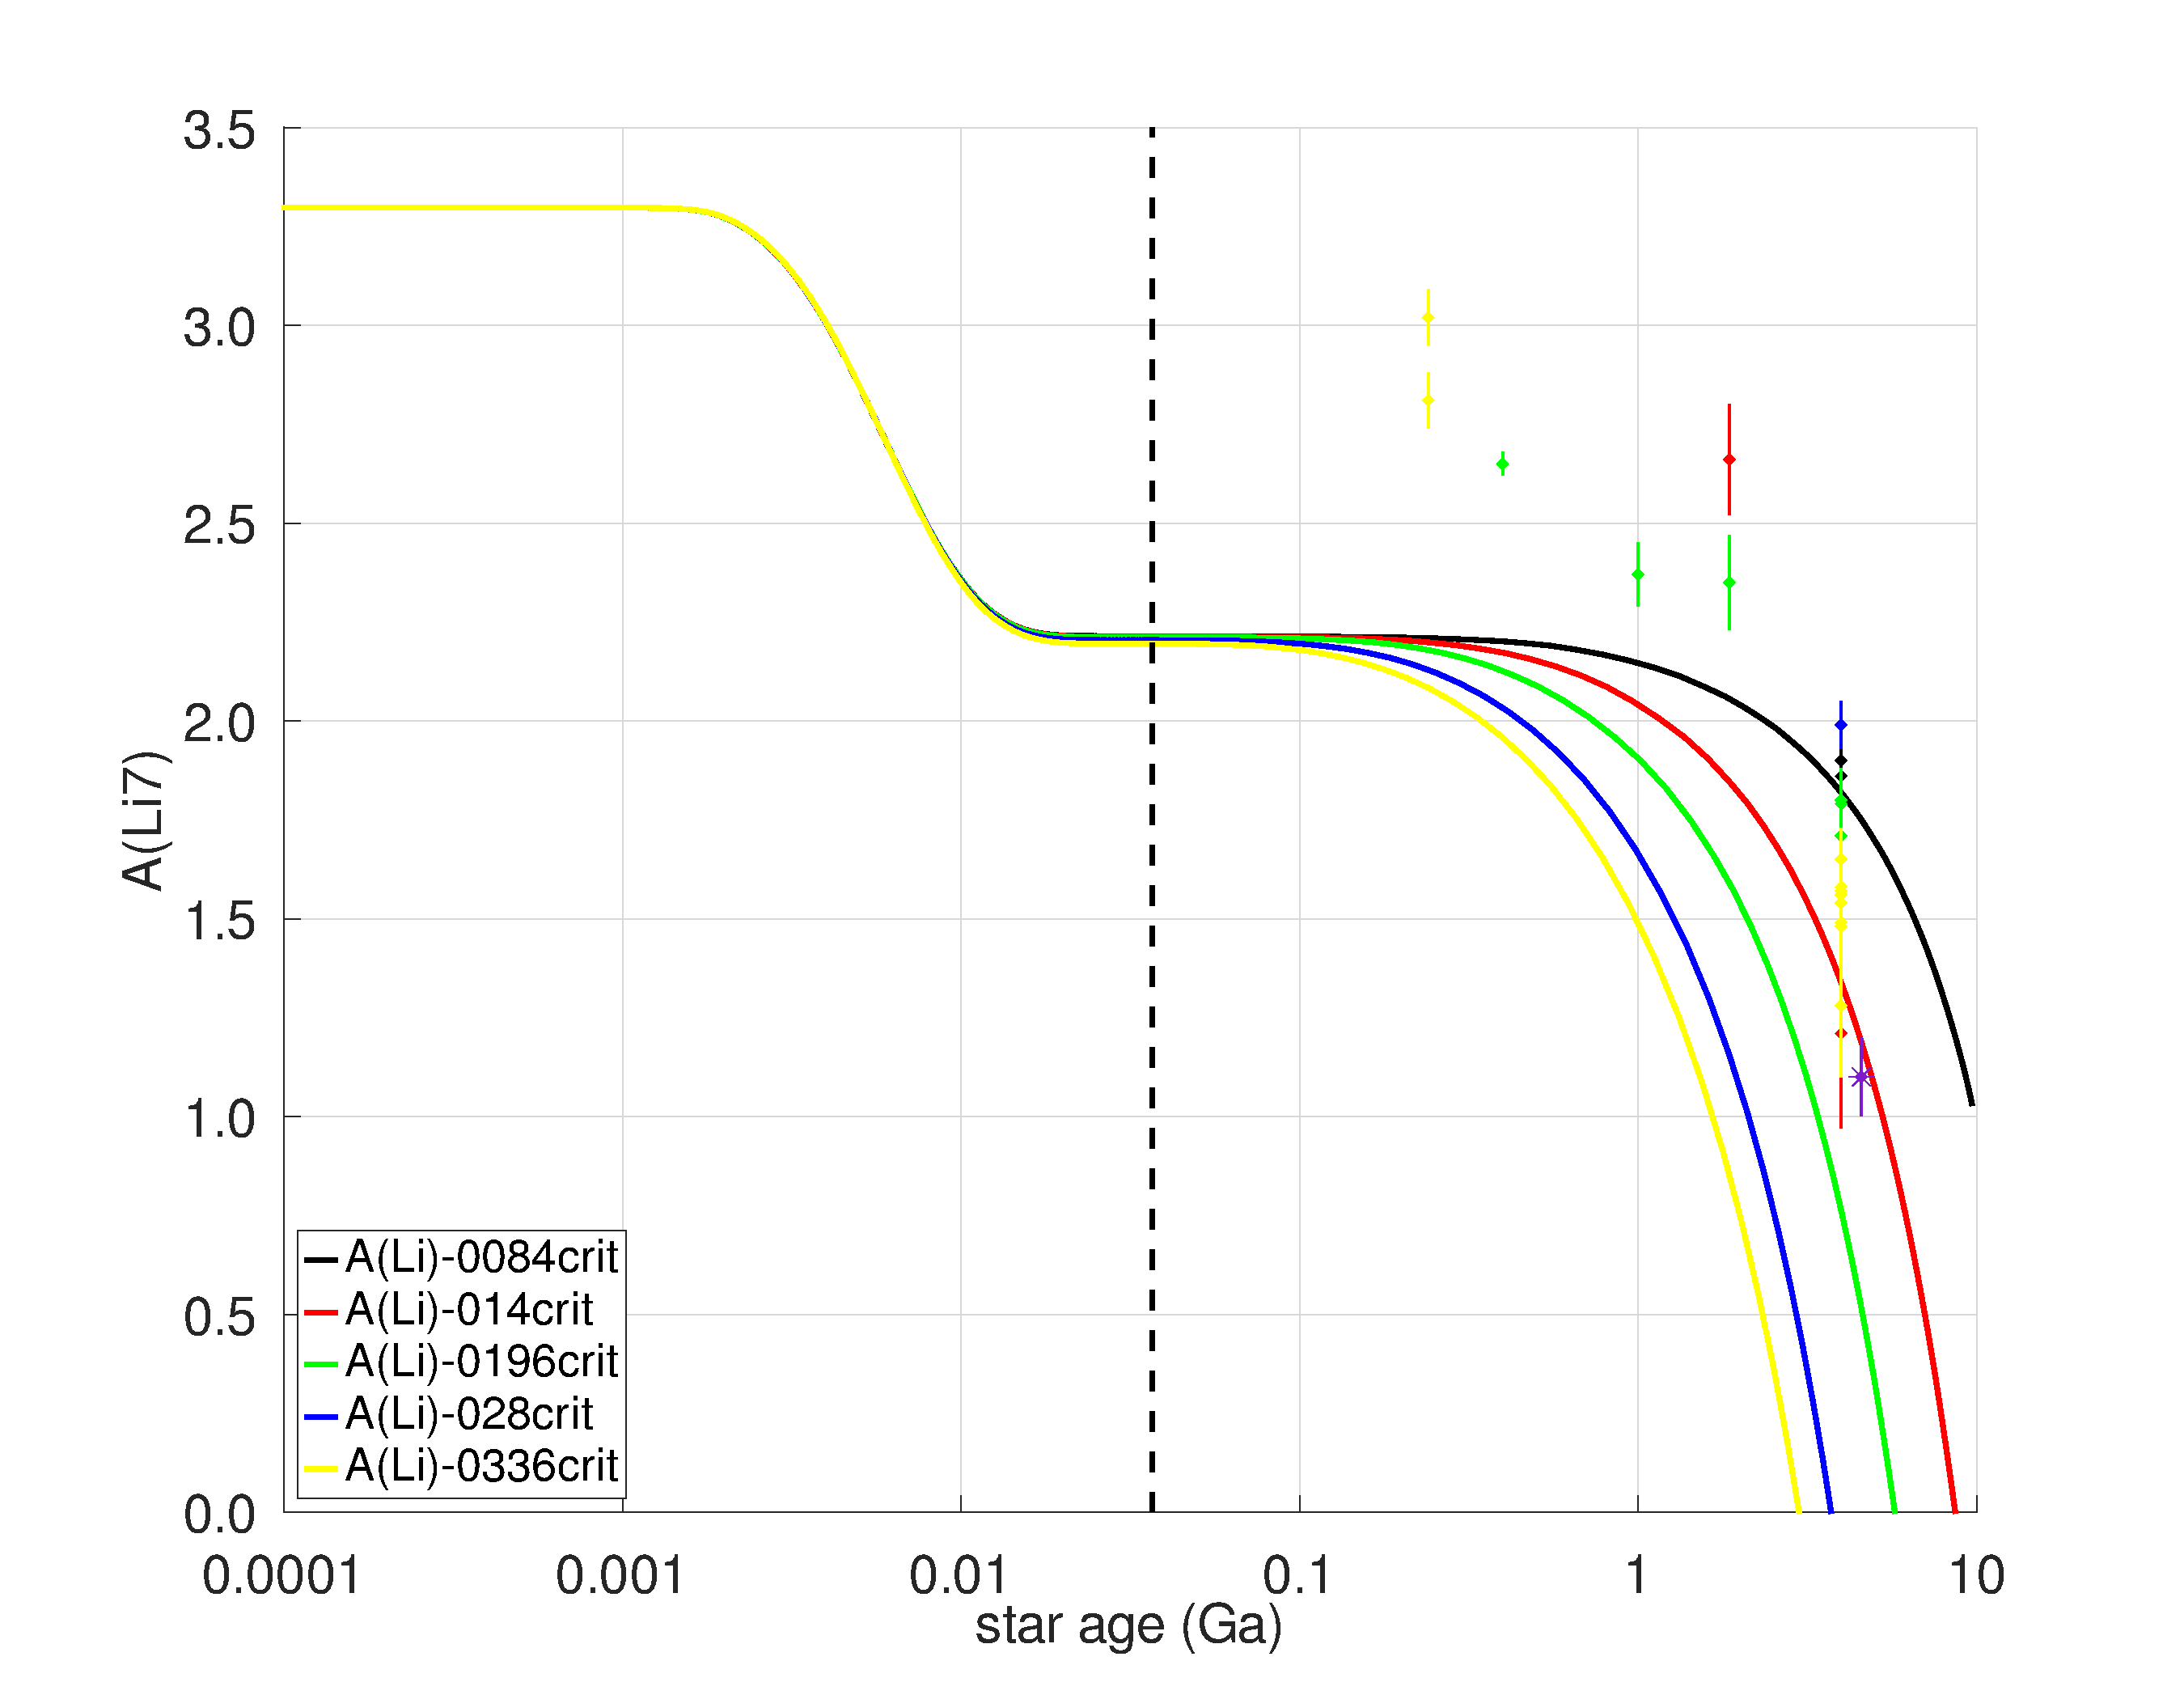
\includegraphics[width=0.7\textwidth]{img/paper2/li_var_vel_0_0g_0.pdf}
	\caption{Se representa la relación entre la abundancia superficial del isotope[7]{Li} y el isotope[1]{H} en función del tiempo para varios modelos de 1 $\msun$ sin campo magnético. El modelo de referencia, propuesto por \cite{Choi2016}, está representado por la línea negra continua. Los modelos adicionales con tasas de rotación iniciales que van de 0.0084 a 0.0336 se ilustran con las líneas restantes. Las abundancias superficiales de Li para el Sol actual, indicadas por una estrella púrpura, se basan en el estudio de \cite{Asplund2009}. La línea vertical discontinua corresponde a la Secuencia Principal de Edad Cero (ZAMS).}
	\label{fig:li_var_vel_0g_ii}
\end{figure}

\begin{figure}
	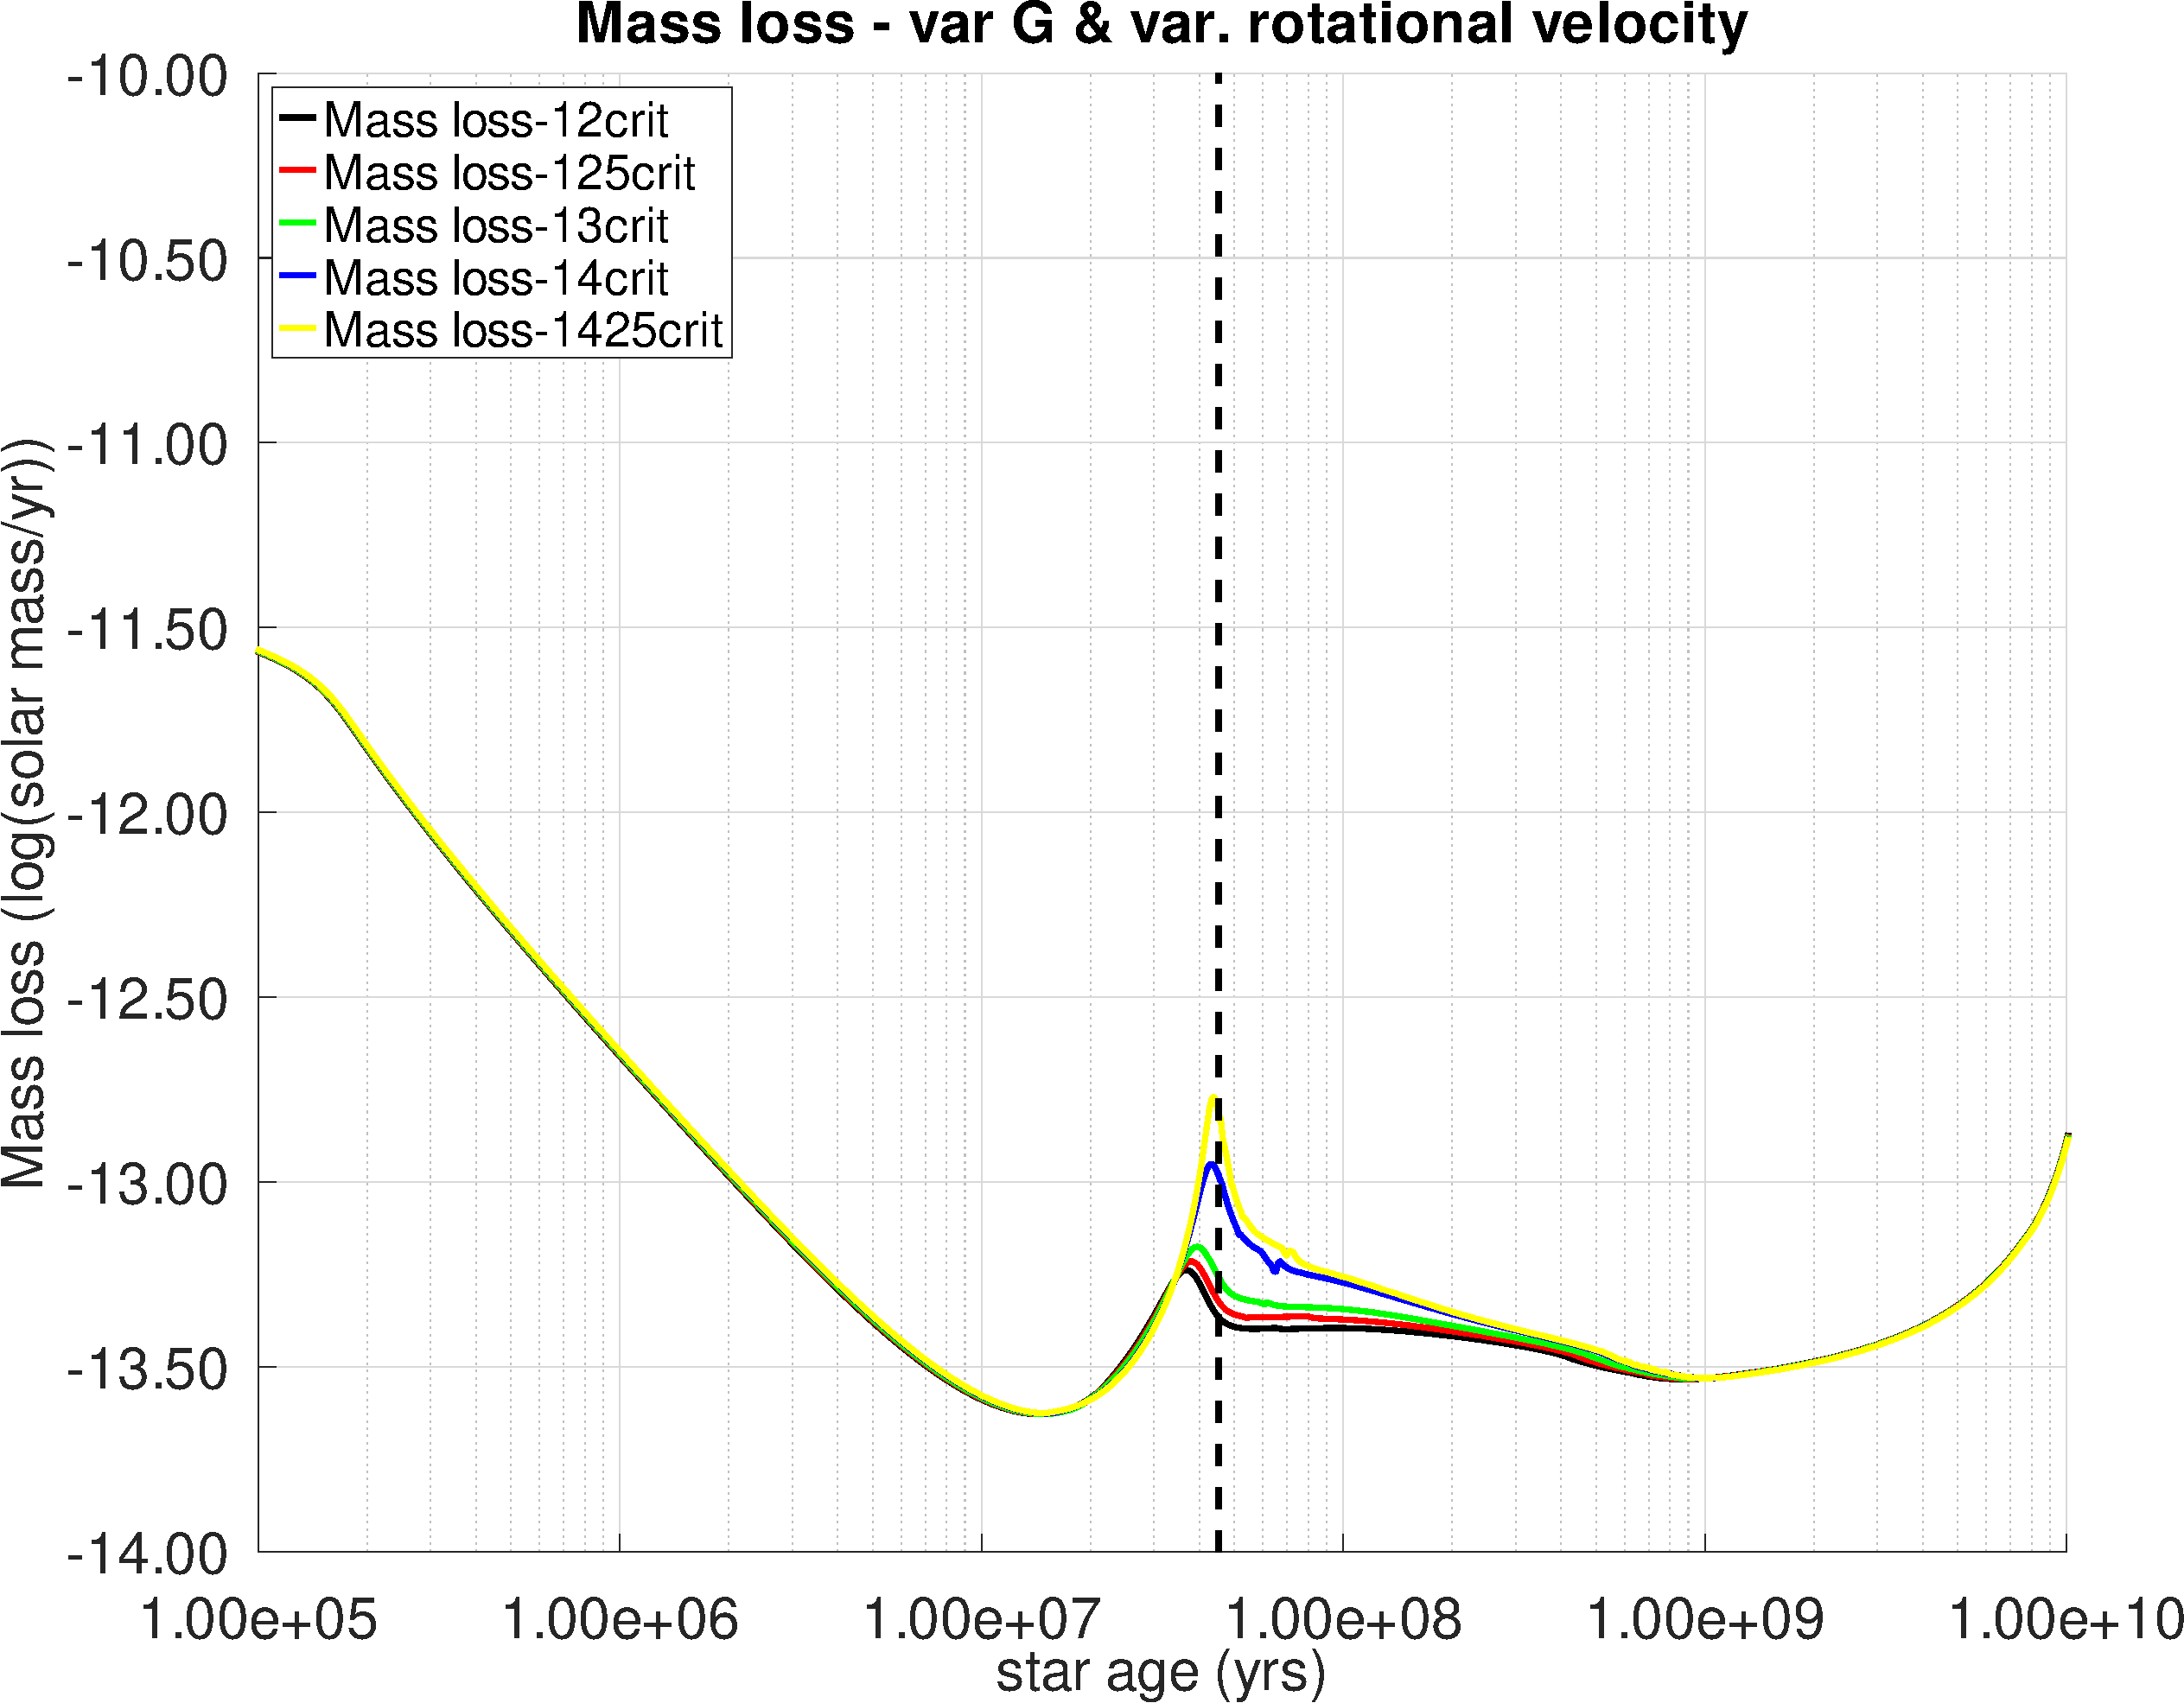
\includegraphics[width=0.7\textwidth]{img/paper2/mdot_var_vel_g3.pdf}
	\caption{Evolución de la pérdida de masa $\Dot{M}$ en función del tiempo para varios modelos de 1 $\msun$. Los modelos incluyen intensidad de campo magnético variable y rotación inicial con $\omegaini$ entre 0.12 y 0.1425. La línea vertical discontinua hace referencia a la ZAMS.}
	\label{fig:mdot_var_vel_g3}
\end{figure}


\begin{figure}
	\centering
	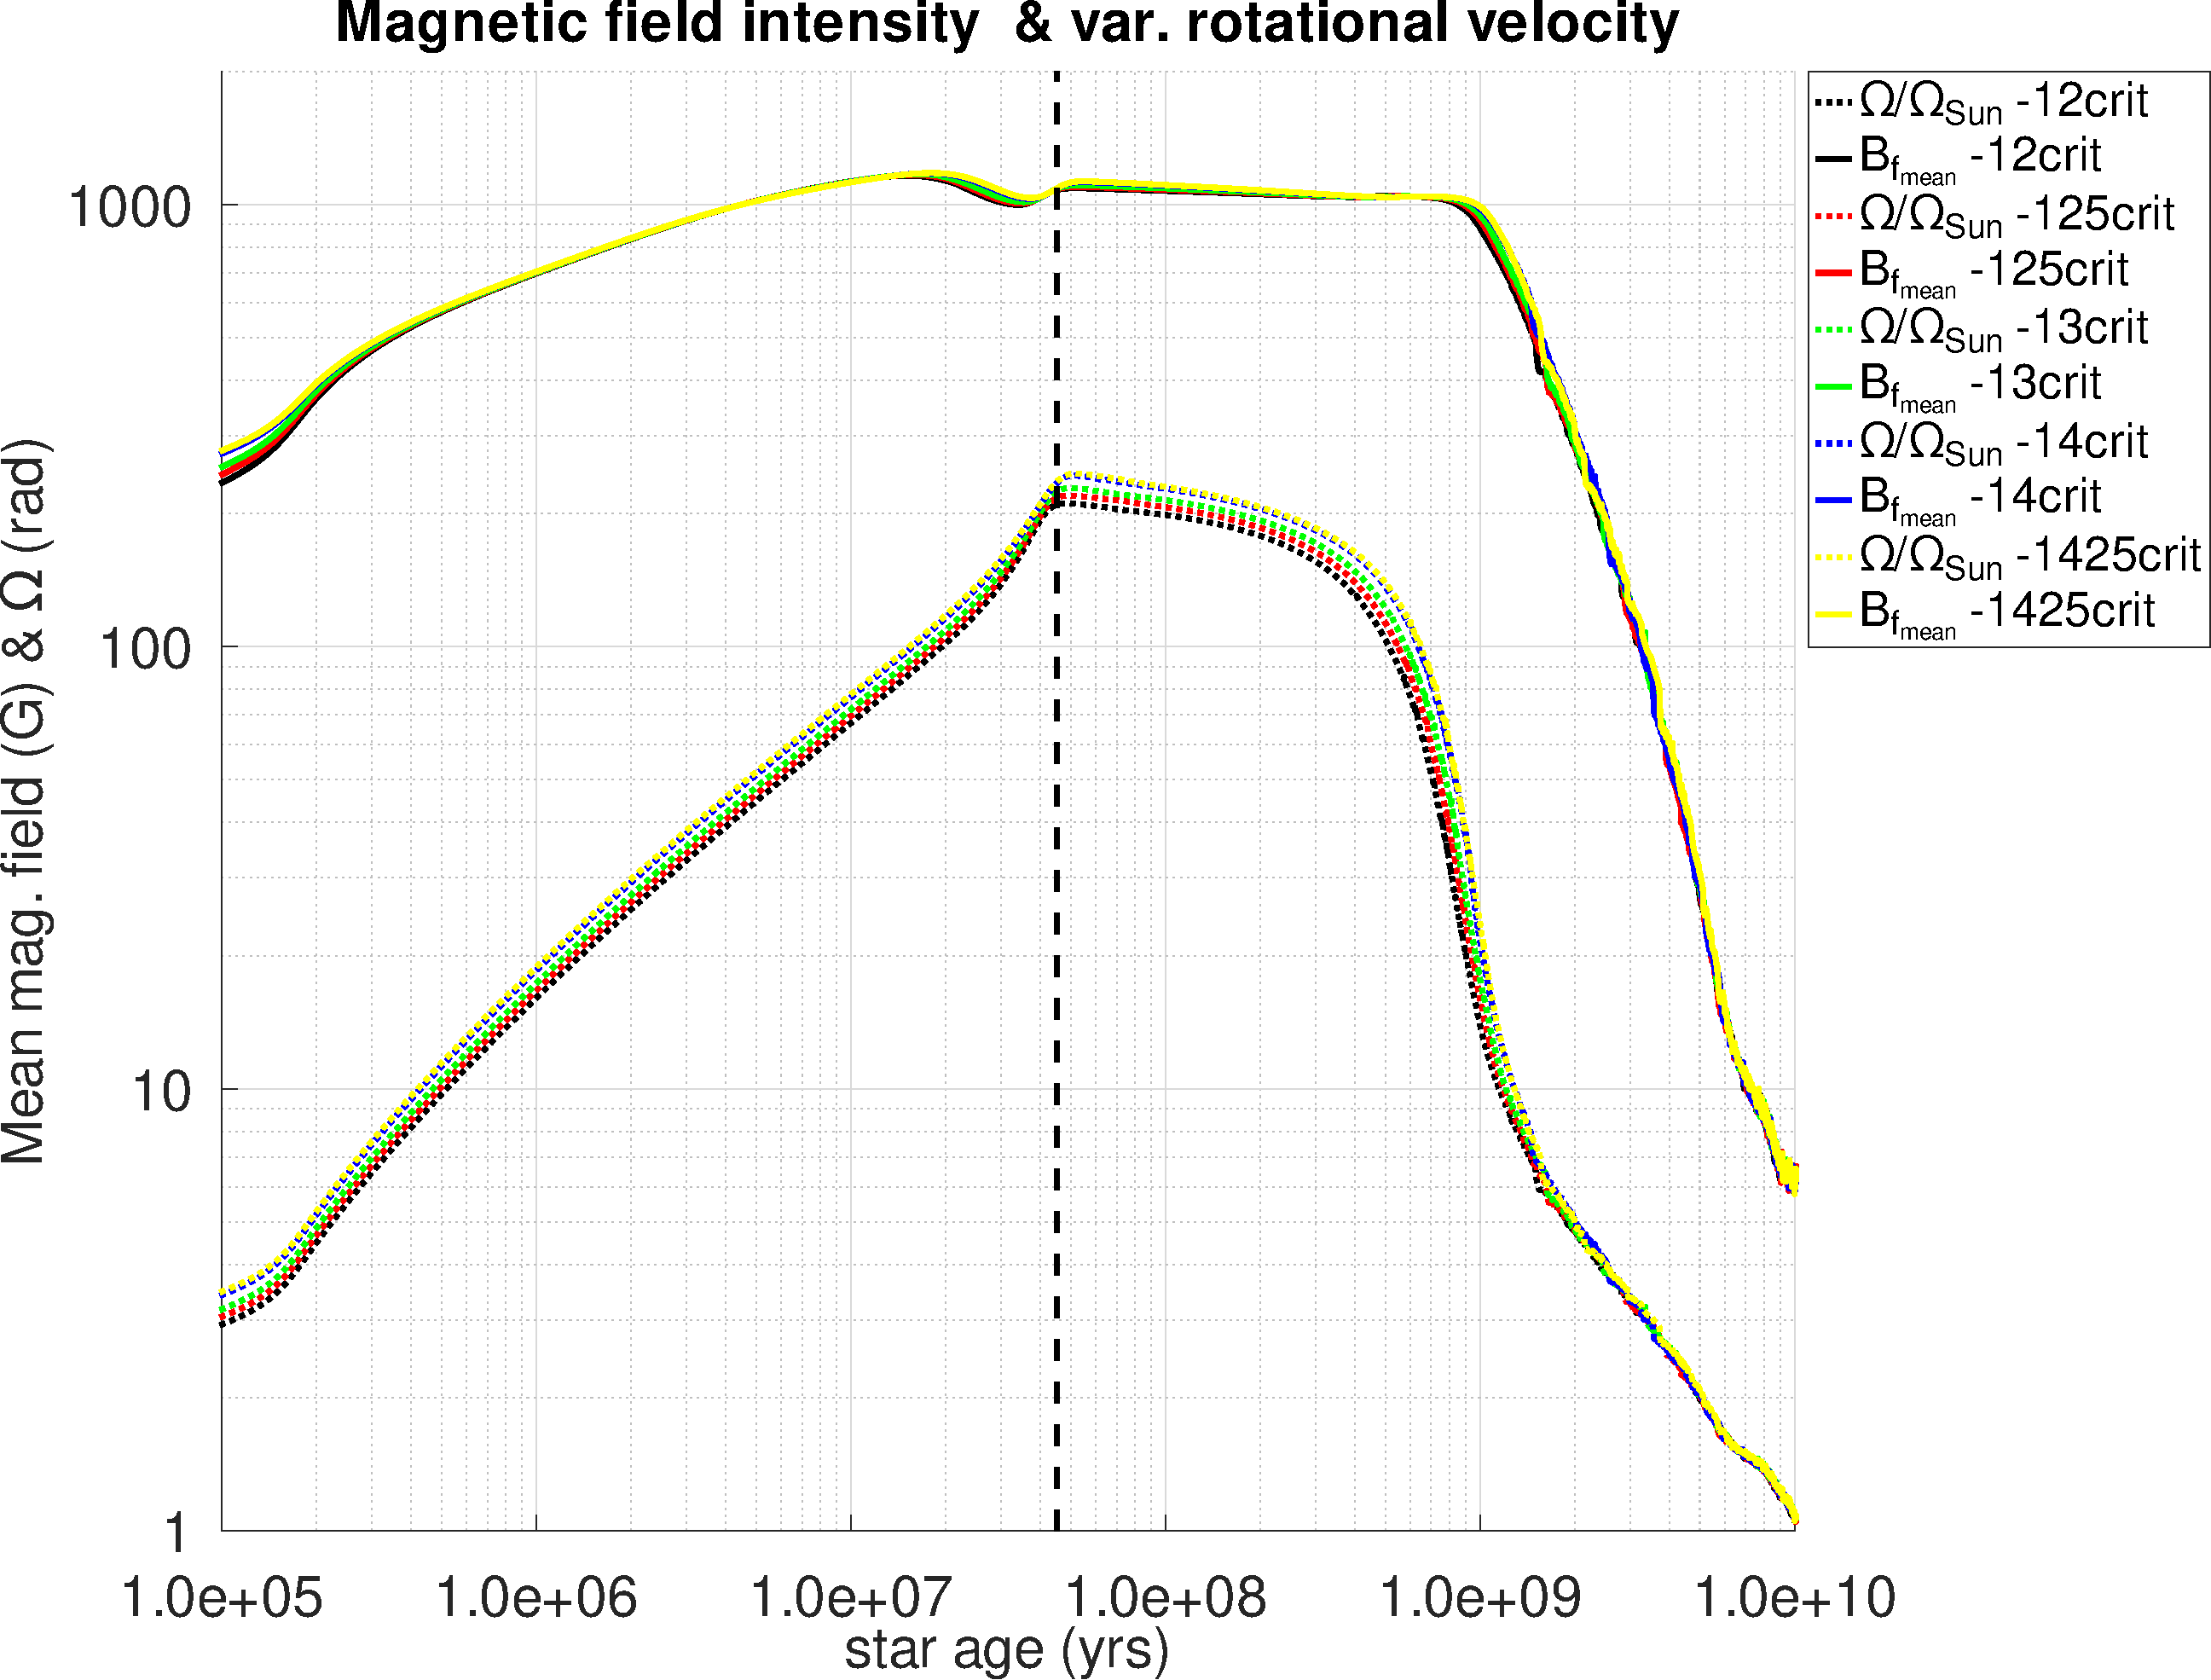
\includegraphics[width=0.7\textwidth]{img/paper2/mag_field_var_vel_g3.pdf}
	\caption{La evolución de la intensidad del campo magnético, en función del tiempo y $\omegaini$ para varios modelos de 1 $\msun$. Los modelos incluyen una rotación inicial con $\omegaini$ entre 0.12 y 0.1425. Las líneas continuas representan la intensidad del campo magnético, mientras que las líneas de puntos representan la evolución angular de la estrella. La línea vertical discontinua hace referencia a la ZAMS.}
	\label{fig:mag_field_var_vel_g3}
\end{figure}

En la Figura \ref{fig:rot_vel_var_vel_var_g3} se representan los perfiles de rotación de las estrellas para la superficie y para el fondo de la envoltura convectiva. Muestra cómo la velocidad angular aumenta de valor a medida que la estrella disminuye de radio a lo largo del PMS. Durante esta etapa de su evolución, la estrella tiene una estructura casi convectiva, como puede verse en la figura \ref{fig:cz_var_vel_var_g3}. A medida que se acerca a una edad de $\approx 10^6$ años, la zona convectiva de la estrella comienza a reducir su tamaño y el núcleo de la estrella alcanza las condiciones de temperatura, presión y densidad necesarias para desarrollar un núcleo radiativo. A su vez, la diferencia en las velocidades angulares de los distintos modelos se hace más evidente, siendo mayor en aquellos que fueron inicializados con una velocidad angular inicial más alta. Este hecho implica que la pérdida de masa también es mayor en aquellas estrellas que rotan más rápido. Como hemos descrito anteriormente, una mayor pérdida de masa implica también una mayor pérdida de momento angular. Los efectos combinados de los aumentos de la temperatura efectiva, la velocidad angular y la pérdida de masa hacen que la intensidad del campo magnético alcance su máximo en la fase de aproximación de la ZAMS (véase la figura \ref{fig:mag_field_var_vel_g3}). Observamos que los modelos con menor velocidad angular generalmente terminan exhibiendo valores más altos para la abundancia de Li en la superficie (ver Figuras~ \ref{fig:li_var_vel_var_g_3}, \ref{fig:grid_li_var_vel} \& \ref{fig:grid_li_var_g}).\par

Para los modelos en los que obtenemos valores de A(Li) en sintonía con los del Sol ($\omegaini$ = 0.14 y 0.1425), tenemos en cambio medidas para el $\Omega$ y $B$ que no están en sintonía con los solares respectivos. La velocidad de rotación de la superficie del Sol es de 2km/s con un error mínimo de 3m/s, y la intensidad media del campo magnético es de 1G. Para la simulación con $\omegaini$=0.1425, obtenemos una velocidad de rotación en el ecuador de 4.72 km/s. Aunque se trata de una medida del mismo orden de magnitud, representa una desviación del 235\%. Para la intensidad media del campo magnético tenemos 36.9G, muy lejos del valor de referencia.\par

Como se describe en la sección \ref{mod_mb}, la rutina MB, que se activa cuando la estrella desarrolla un núcleo radiativo y una zona convectiva sobre él (ver Figura \ref{fig:mb_act_var_vel_g3}), distribuyó la cantidad total de LMA calculada según la Ec.~\ref{eq:k_jdot} entre las distintas capas que componían la CZ. En la Figura \ref{fig:cz_var_vel_var_g3} podemos observar la evolución de la CZ más externa normalizada con respecto al radio de la estrella para varios modelos de 1 $\msun$. De acuerdo con los modelos establecidos de evolución estelar, en una estrella de tipo solar la CZ cubre prácticamente en su totalidad gran parte del PMS. A partir de la ZAMS, su tamaño comienza a disminuir gradualmente en una primera fase y luego se hace más pronunciado en torno a los $4.0x10^8$ años de edad. Como puede verse en la figura \ref{fig:rot_vel_var_vel_var_g3}, la estrella, tras alcanzar su velocidad angular máxima al pasar por la ZAMS, comienza a desacelerar debido al frenado magnético.\par

Es la presencia del MB la que impide que la estrella siga aumentando su velocidad angular. De este modo, la destrucción del Li se ve atenuada por una menor velocidad de rotación. Los modelos comienzan a desacelerarse gradualmente una vez superada la ZAMS y durante el periodo inicial de su estancia en la EM. La intensidad del campo magnético se mantiene cerca de su máximo, disminuye ligeramente y luego se reduce de forma más acusada. Su comportamiento refleja el de la evolución de la velocidad angular, consecuencia de los efectos de la MB. El proceso de desaceleración continúa progresivamente hasta que, en torno a la edad actual del Sol, se obtienen valores de velocidad angular muy similares a los del Sol. La desaceleración conduce a un menor efecto de las fuerzas centrífugas, lo que permite una contracción del radio de la estrella y, por tanto, un menor tamaño del CZ. Además, una menor velocidad angular tiene un efecto sobre la intensidad del campo magnético, como puede verse en la Figura \ref{fig:mag_field_var_vel_g3}. El acoplamiento entre la velocidad angular, la intensidad del campo magnético y el radio de la estrella es evidente y coherente.\par

\begin{figure}
	\centering
	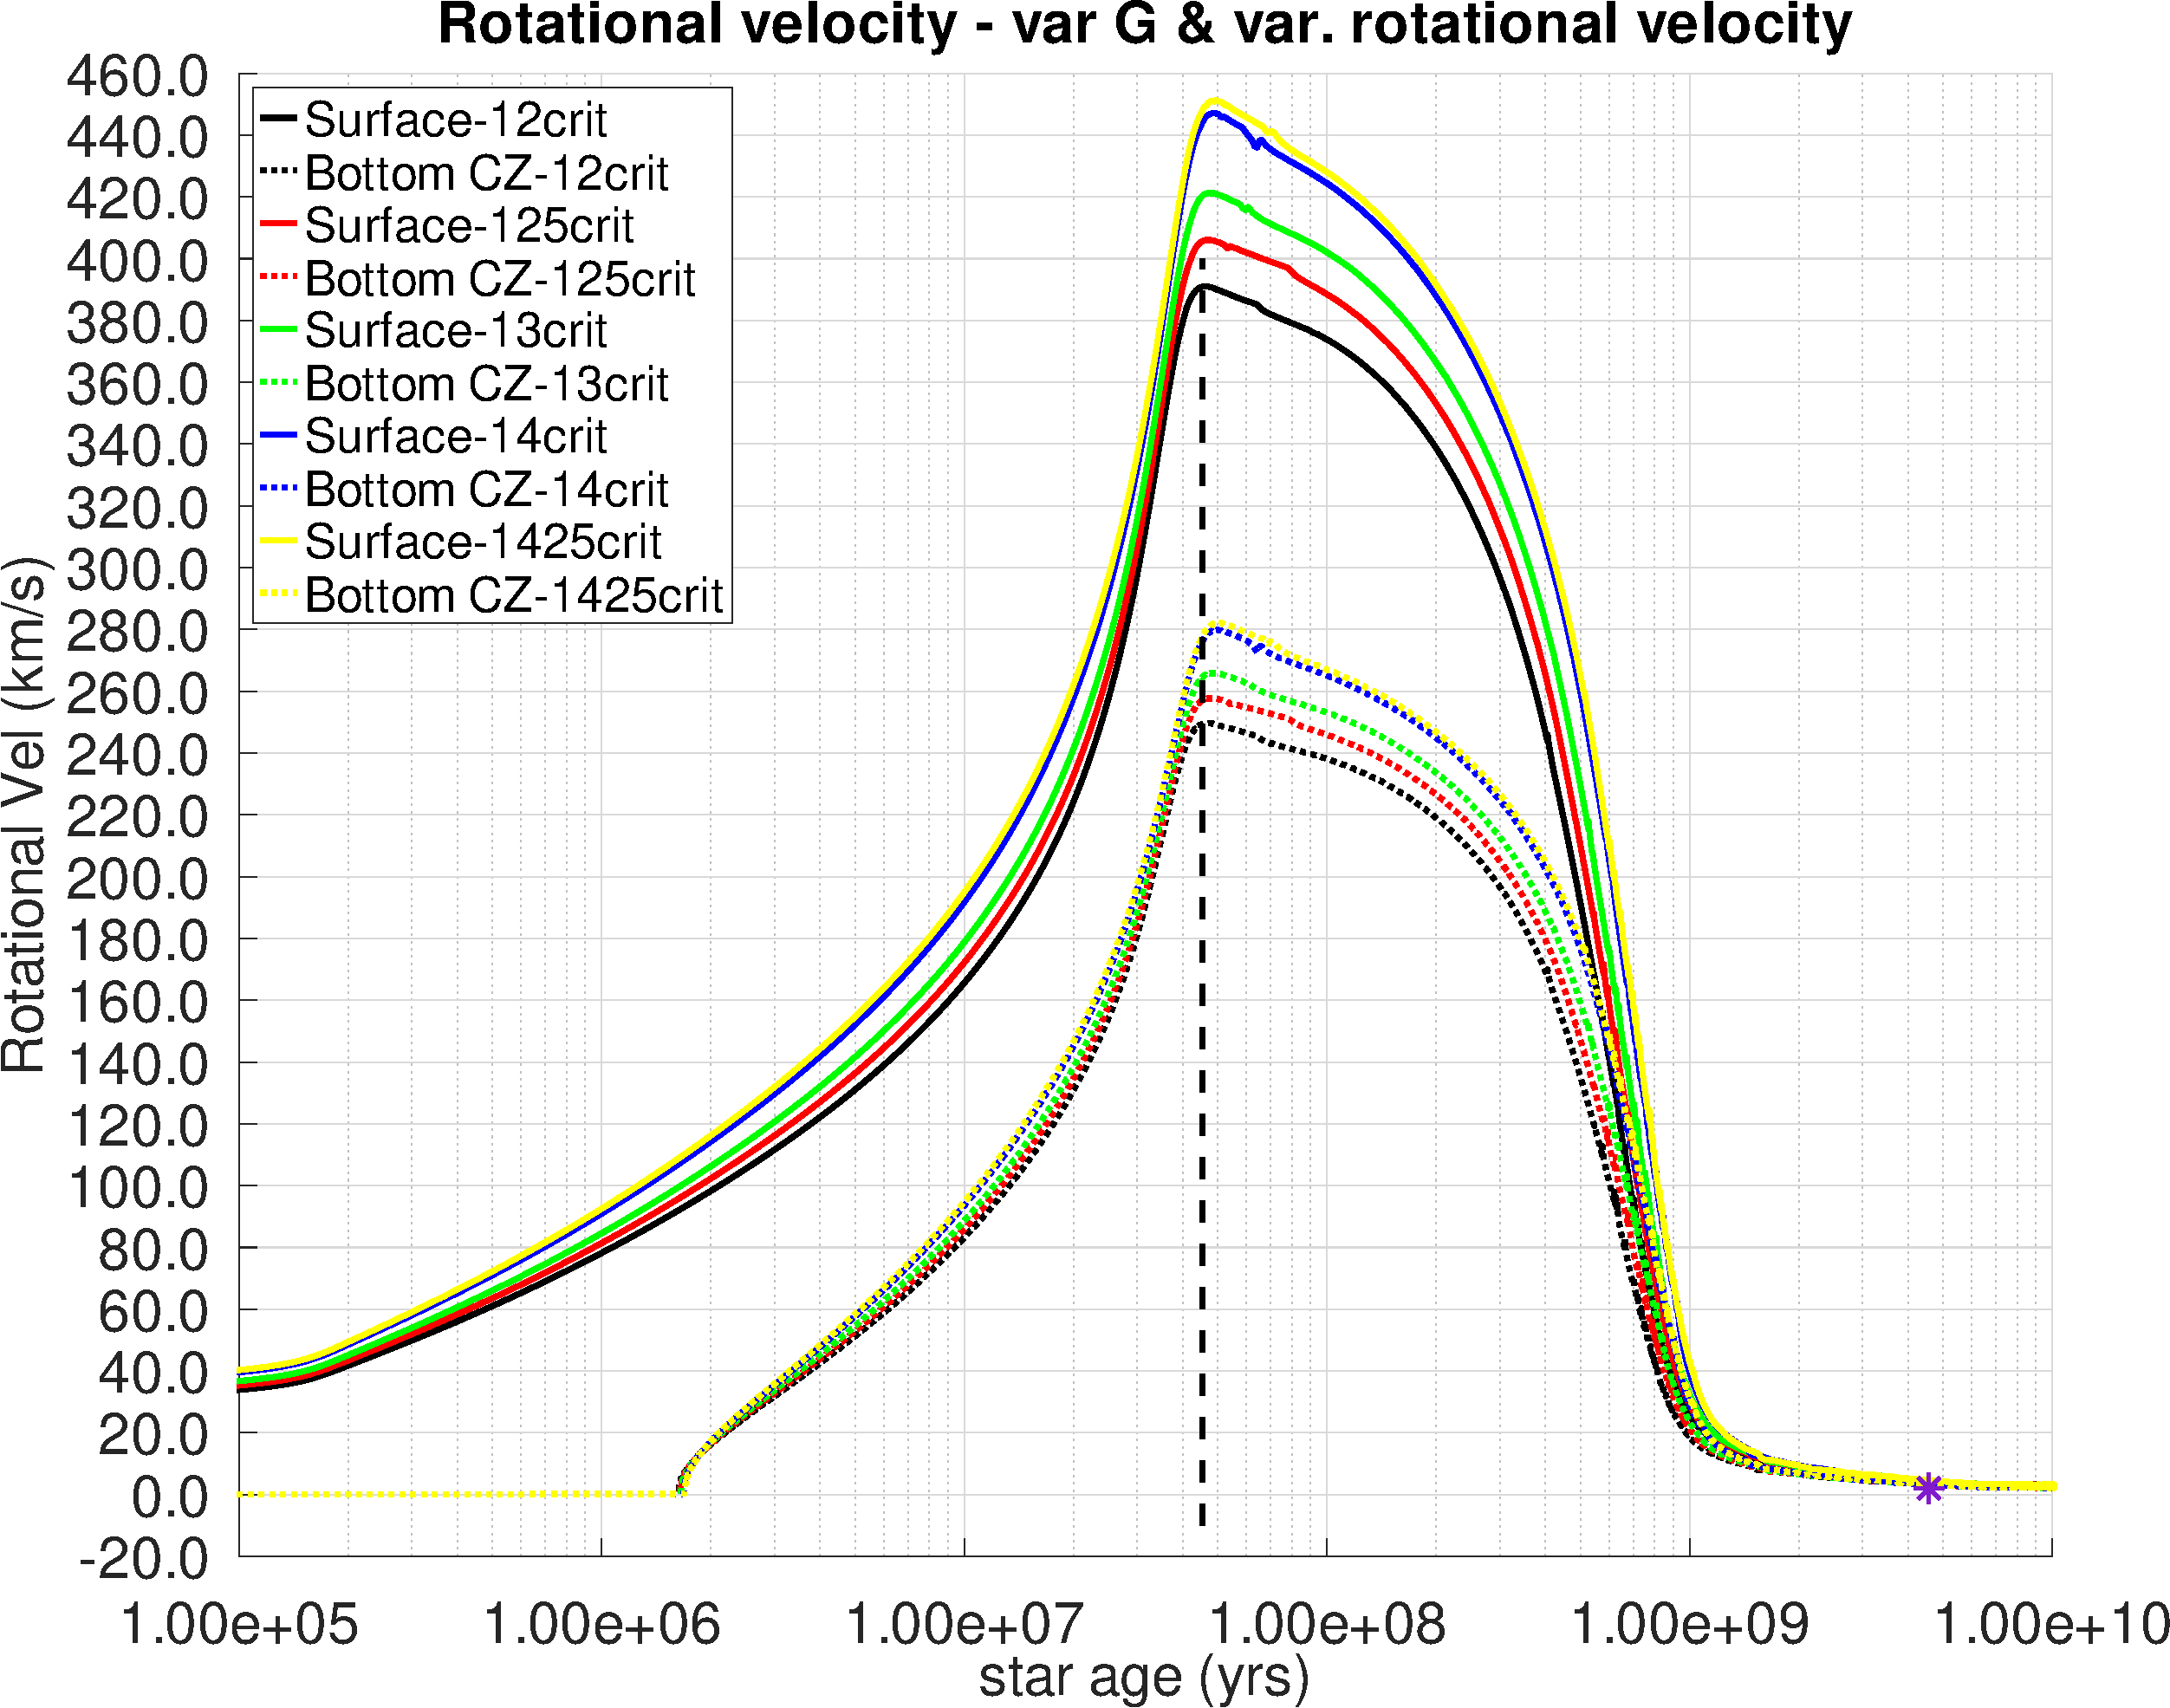
\includegraphics[width=0.7\textwidth]{img/paper2/rot_vel_var_vel_var_g3.pdf}
	\caption{La evolución de la velocidad de rotación de la superficie, en función del tiempo para varios modelos de 1 $\msun$. Los modelos incluyen un campo magnético de intensidad variable, rotación inicial con $\omegaini$ entre 0.12 y 0.1425, respectivamente y MB. La estrella púrpura es la velocidad angular superficial para el Sol actual \cite{Gill2012}. La línea vertical discontinua hace referencia a la ZAMS.}
	\label{fig:rot_vel_var_vel_var_g3}
\end{figure}

\begin{figure}
	\centering
	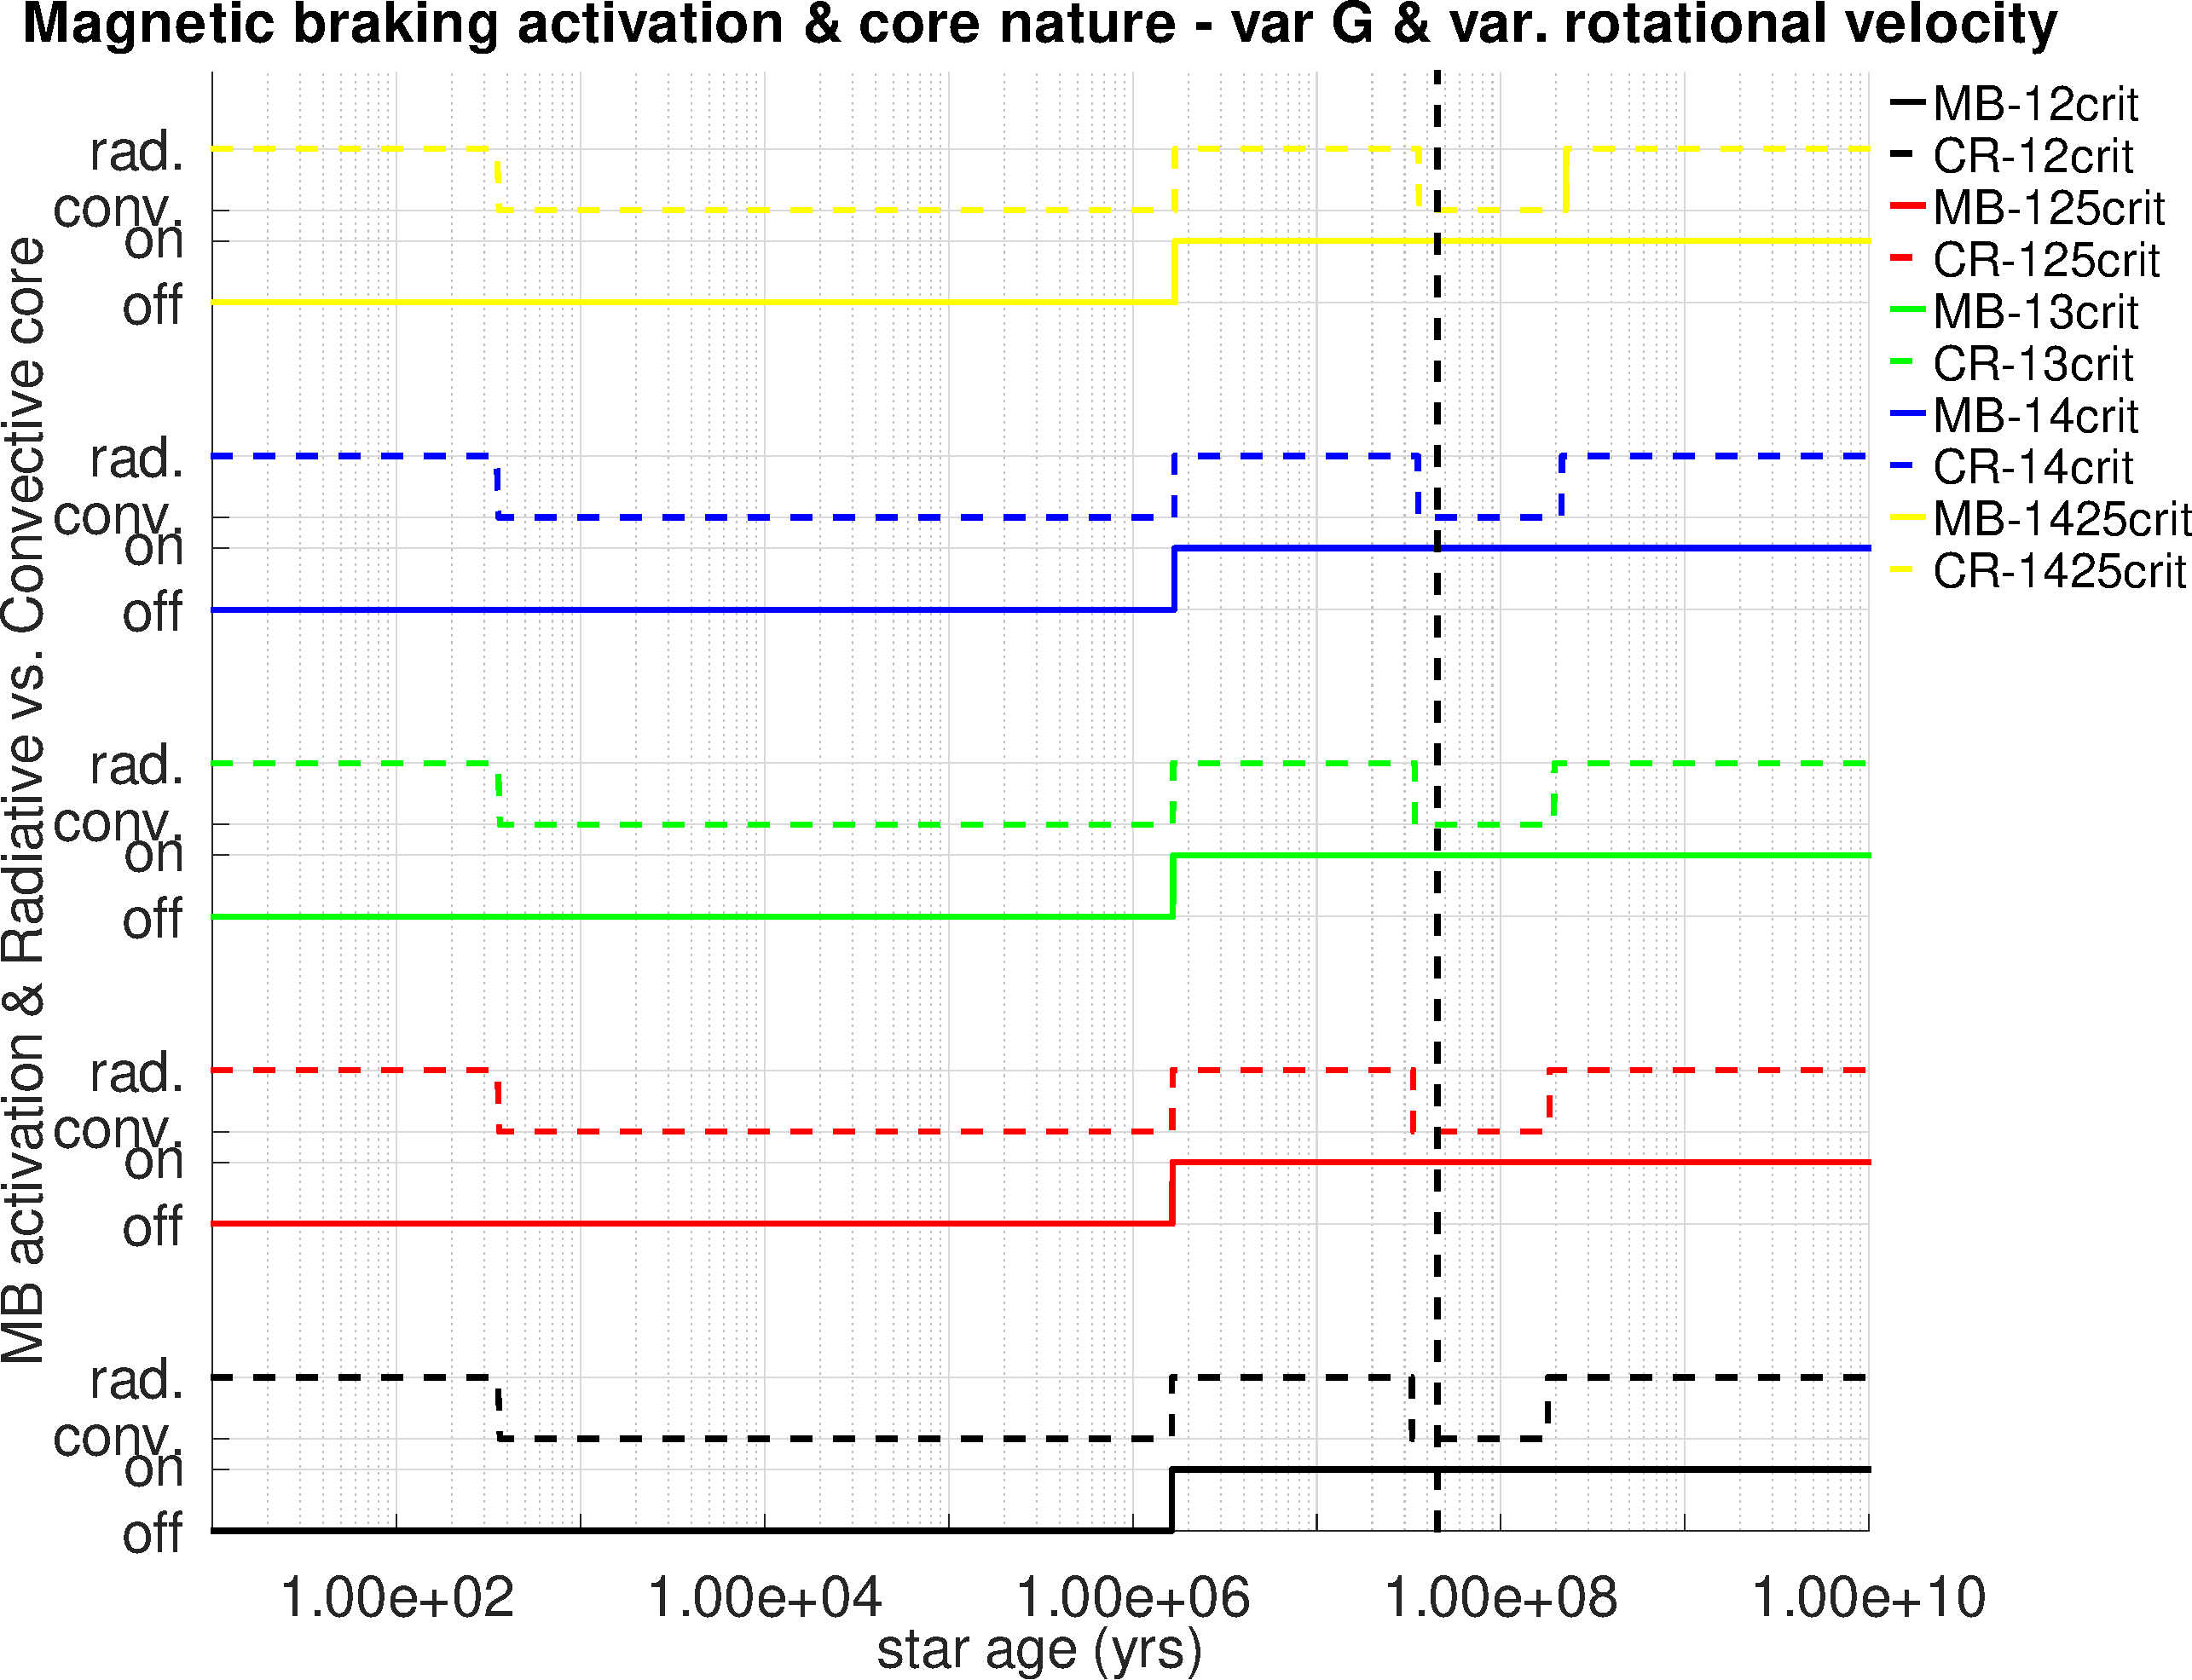
\includegraphics[width=0.7\textwidth]{img/paper2/mb_act_var_vel_g3.pdf}
	\caption{La activación de la rutina de frenado magnético en función de la presencia de un núcleo radiativo. Las líneas continuas señalan la activación (on) y desactivación (off) de la rutina de frenado magnético. Las líneas horizontales discontinuas informan sobre la naturaleza del núcleo de la estrella: radiativo (rad) o convectivo (conv). Por decisión de implementación, una vez activada la rutina, permanece activada incluso si la naturaleza del núcleo de la estrella cambia a convectiva. La línea vertical discontinua hace referencia a la ZAMS.}
	\label{fig:mb_act_var_vel_g3}
\end{figure}

\begin{figure}
	\centering
	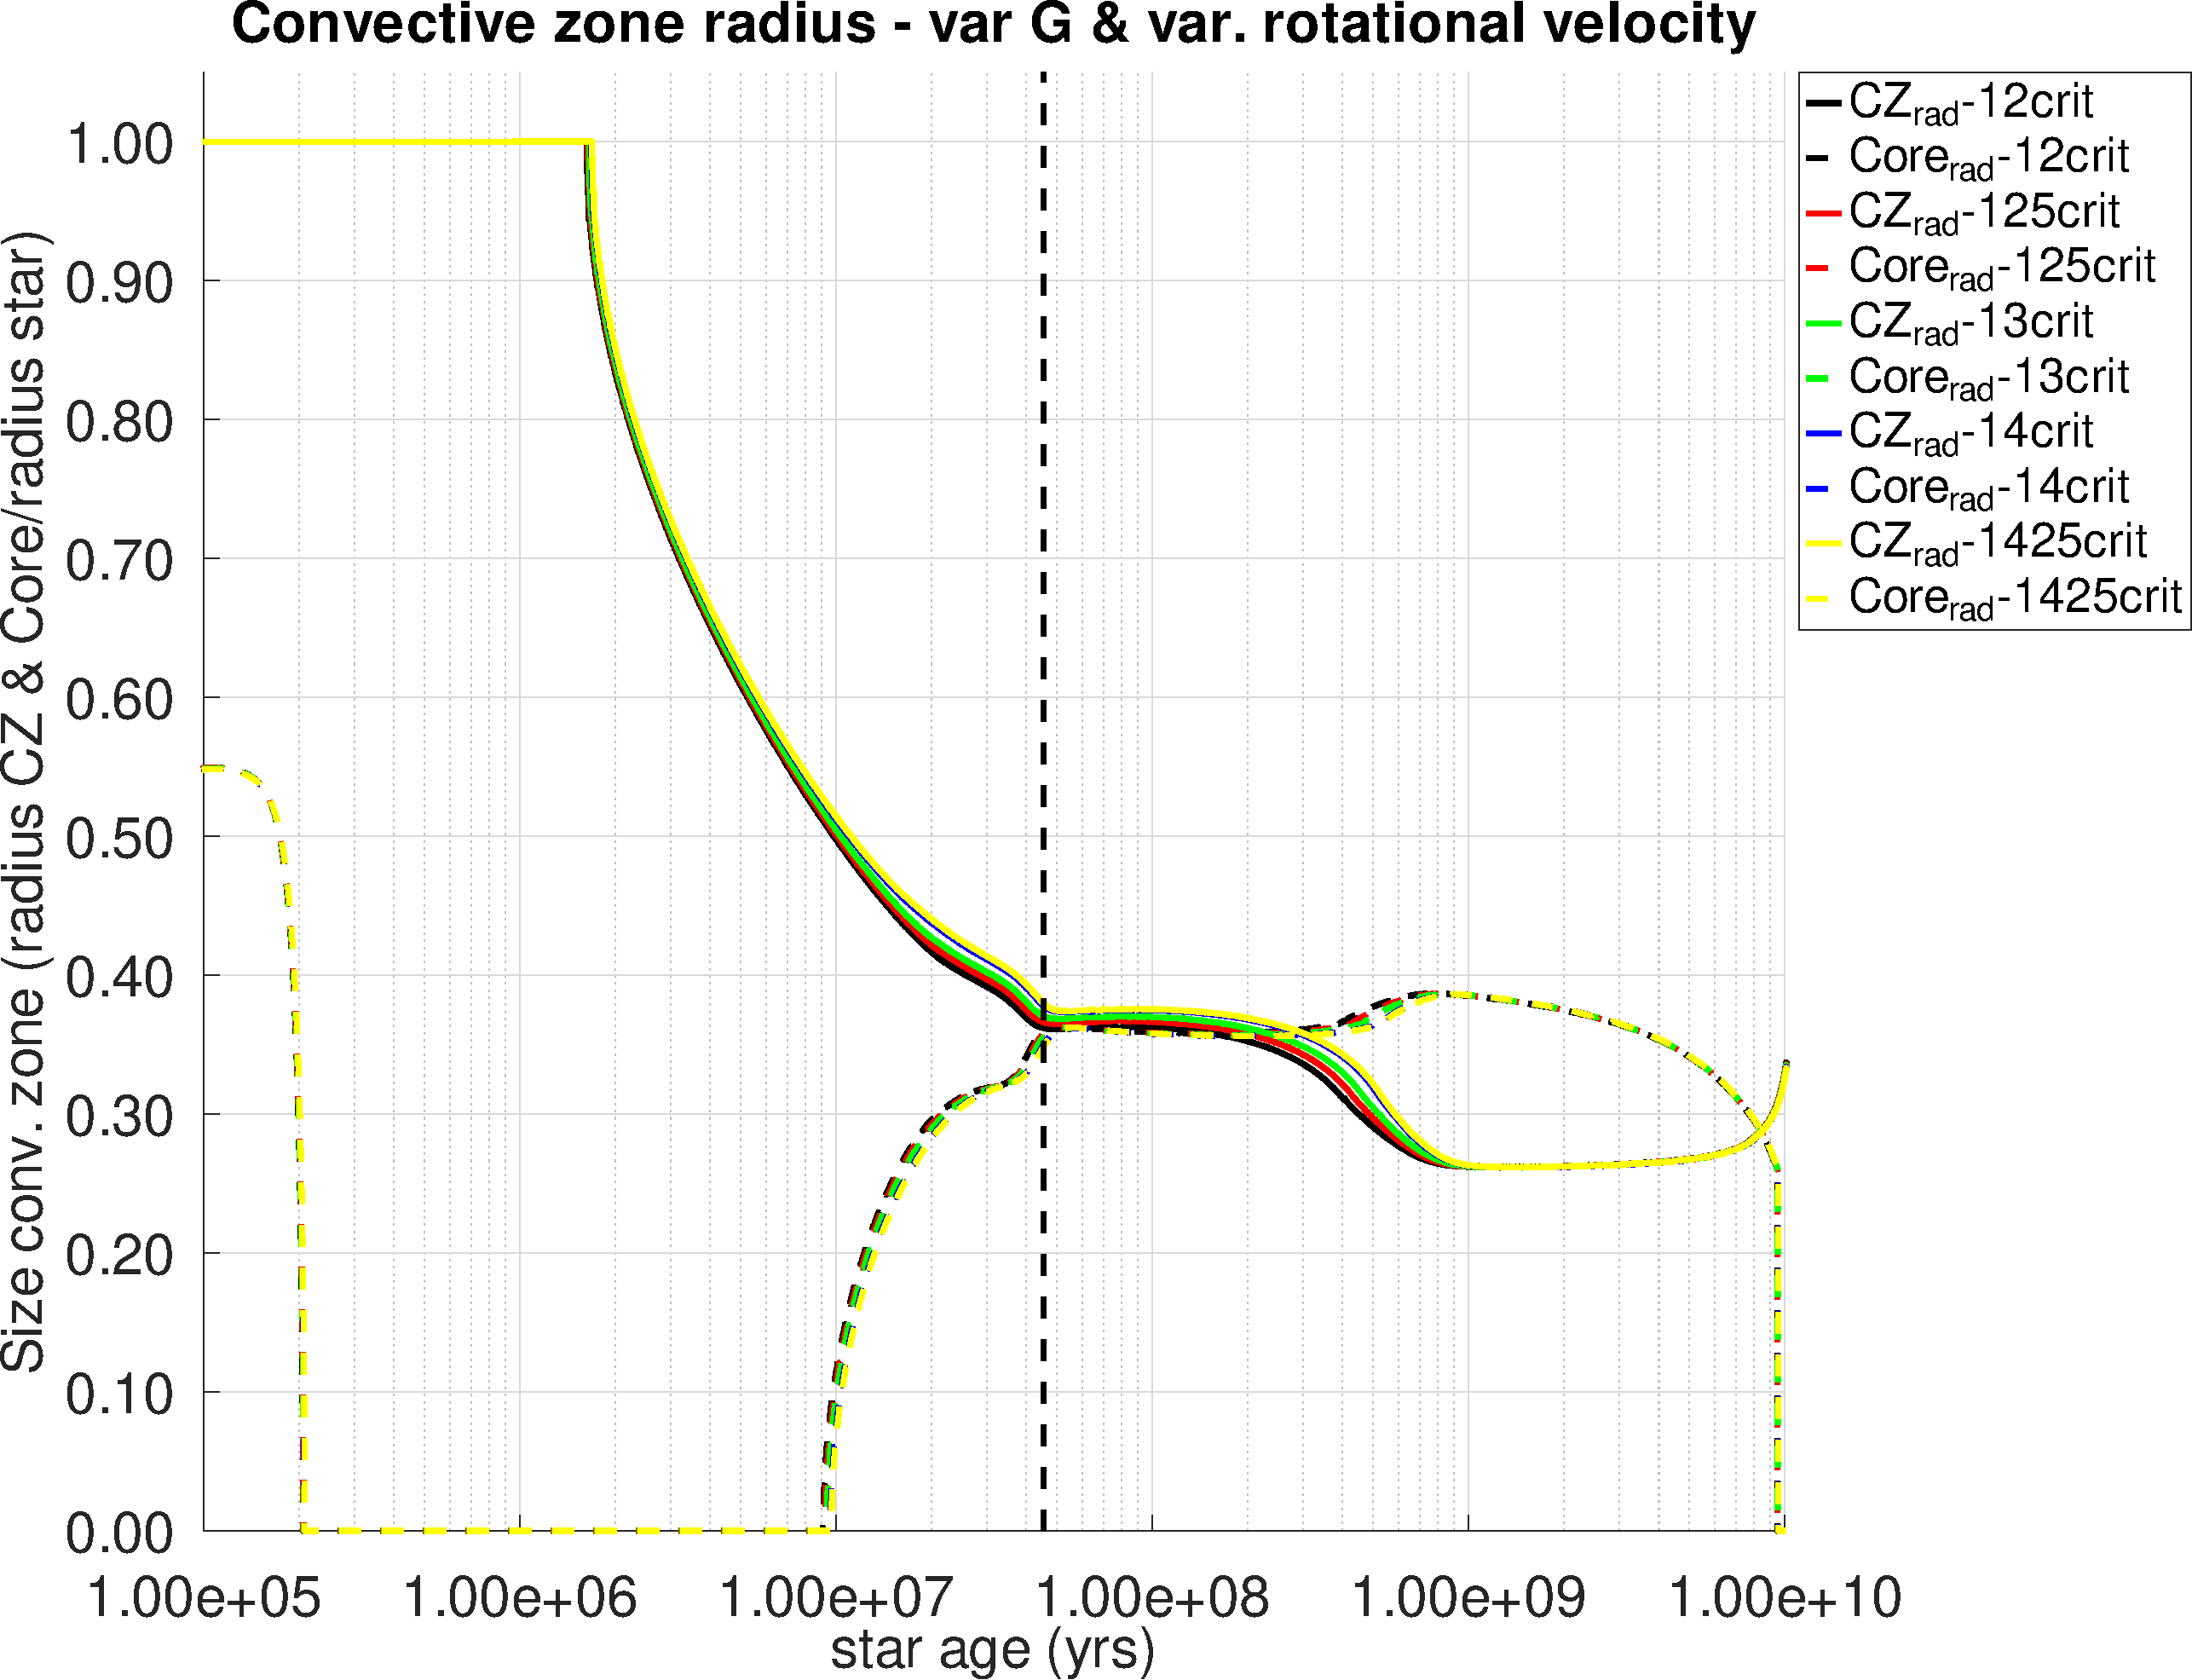
\includegraphics[width=0.7\textwidth]{img/paper2/cz_var_vel_var_g3.pdf}
	\caption{SUSTITUIR POR GRÁFICA MOSTRANDO SOLO LA CZ. Evolución del tamaño de la zona convectiva en función del tiempo para varios modelos de 1 $\msun$. El tamaño se expresa en términos de $\rsun$. Los modelos incluyen un campo magnético de intensidad variable, rotación inicial con $\omegaini$ entre 0.12 y 0.1425. La línea vertical discontinua hace referencia a la ZAMS.}
	\label{fig:cz_var_vel_var_g3}
\end{figure}


\subsection{Evolución del Li con MB de intensidad y $\amlt$ variables}
Los efectos de la rotación y el frenado magnético también pueden observarse en el diagrama H-R y en la evolución del $\amlt$. La inclusión de la rotación implica la aparición de fuerzas centrífugas que afectan tanto a la estructura de la estrella como a la composición química de los distintos estratos que la componen, así como a su temperatura y luminosidad. La rotación diferencial entre los límites del núcleo radiativo y las capas convectivas provoca efectos de mezcla en la denominada tacoclina. Los efectos de esta mezcla y de sus efectos hidrostáticos se rigen por la MLT, en la que el $\amlt$ desempeña un papel fundamental. Como ya se ha dicho, la MLT adolece de la arbitrariedad del valor de $\amlt$. La figura \ref{fig:alpha_mlt_var_vel_g3} muestra cómo evoluciona el parámetro $\amlt$ con el tiempo.\par 

\begin{figure}
	\centering
	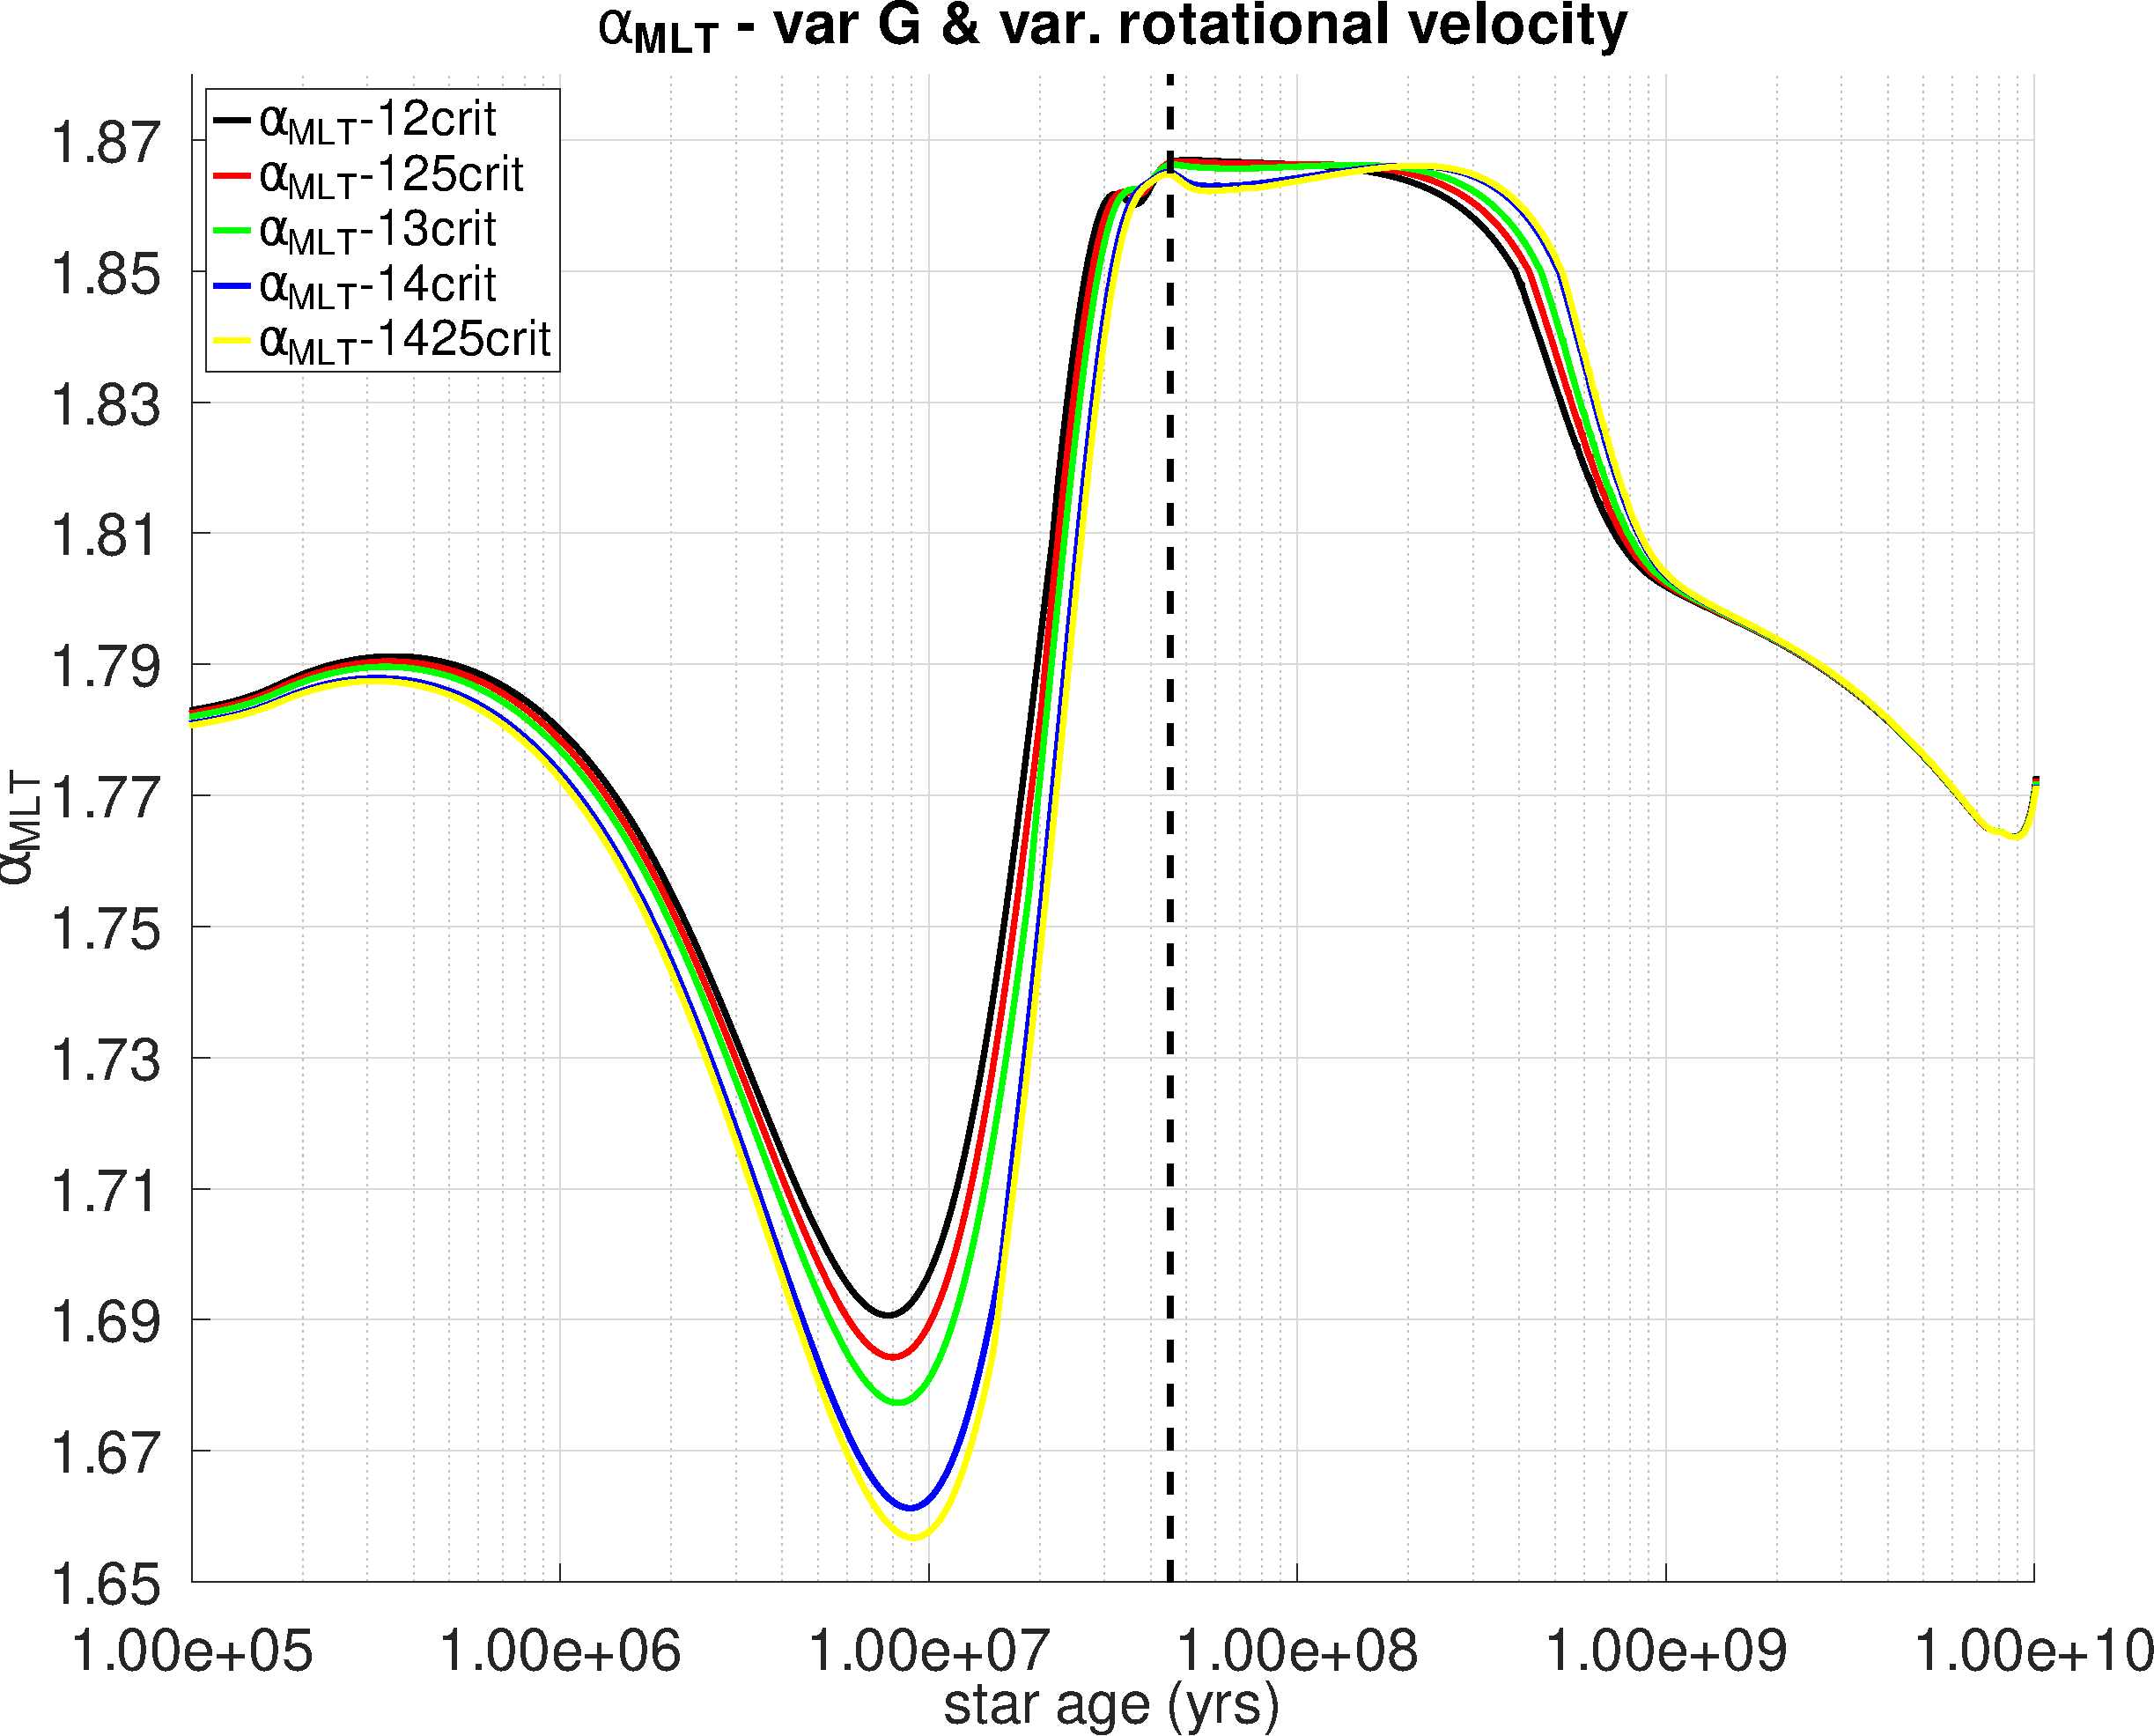
\includegraphics[width=0.7\textwidth]{img/paper2/alpha_mlt_var_vel_g3.pdf}
	\caption{La evolución de $\amlt$, en función del tiempo y $\omegaini$ para varios modelos de 1 $\msun$. Los modelos incluyen una rotación inicial con $\omegaini$ entre 0.12 y 0.1425. La línea vertical discontinua hace referencia a la ZAMS. La estrella púrpura y el rombo son los $\amlt$ dados por \cite{Sonoi2018} y \cite{Samadi2005}, respectivamente.}
	\label{fig:alpha_mlt_var_vel_g3}
\end{figure}

Además, estas mismas fuerzas centrífugas, acentuadas en estrellas con mayor velocidad angular, refuerzan también el oscurecimiento gravitatorio \cite[véase por ejemplo ][]{Eggenberger2012,Paxton2019,Gossage2021}. La fuerza centrífuga hace que la estrella desplace su masa hacia fuera con respecto al eje de rotación, siendo el efecto más pronunciado en las regiones ecuatoriales que en los polos. La consecuencia es que la presión ($\gsurf$) a la que está sometido el gas es menor en las primeras que en las segundas. Este efecto hace que las estrellas que rotan a gran velocidad aparezcan menos densas ($\rho$), menos luminosas ($L$) y, por tanto, con una temperatura efectiva ($\teff$) más baja a medida que se acercan a la ZAMS (véase la figura \ref{fig:hr_var_vel_var_g_z13}). Si comparamos el modelo no rotatorio (línea sólida negra en la Figura \ref{fig:hr_var_vel_0g}) con los rotatorios, podemos reconocer que al final del PMS, estos últimos alcanzan la ZAMS con un $\teff$ menor que los primeros. Esto también repercute en la evolución de $\amlt$ ya que, como se ha comentado anteriormente, en nuestro modelo su valor depende proporcionalmente de $\teff$ y $\gsurf$. Ambos parámetros son comparativamente menores en las estrellas que giran más rápido que en las que lo hacen más despacio. Como consecuencia $\amlt$ arroja un valor menor en su evolución temporal en aquellas fases en las que la estrella rota más rápido, siendo este efecto más acentuado en la aproximación ZAMS.\par

\begin{figure}
	\centering
	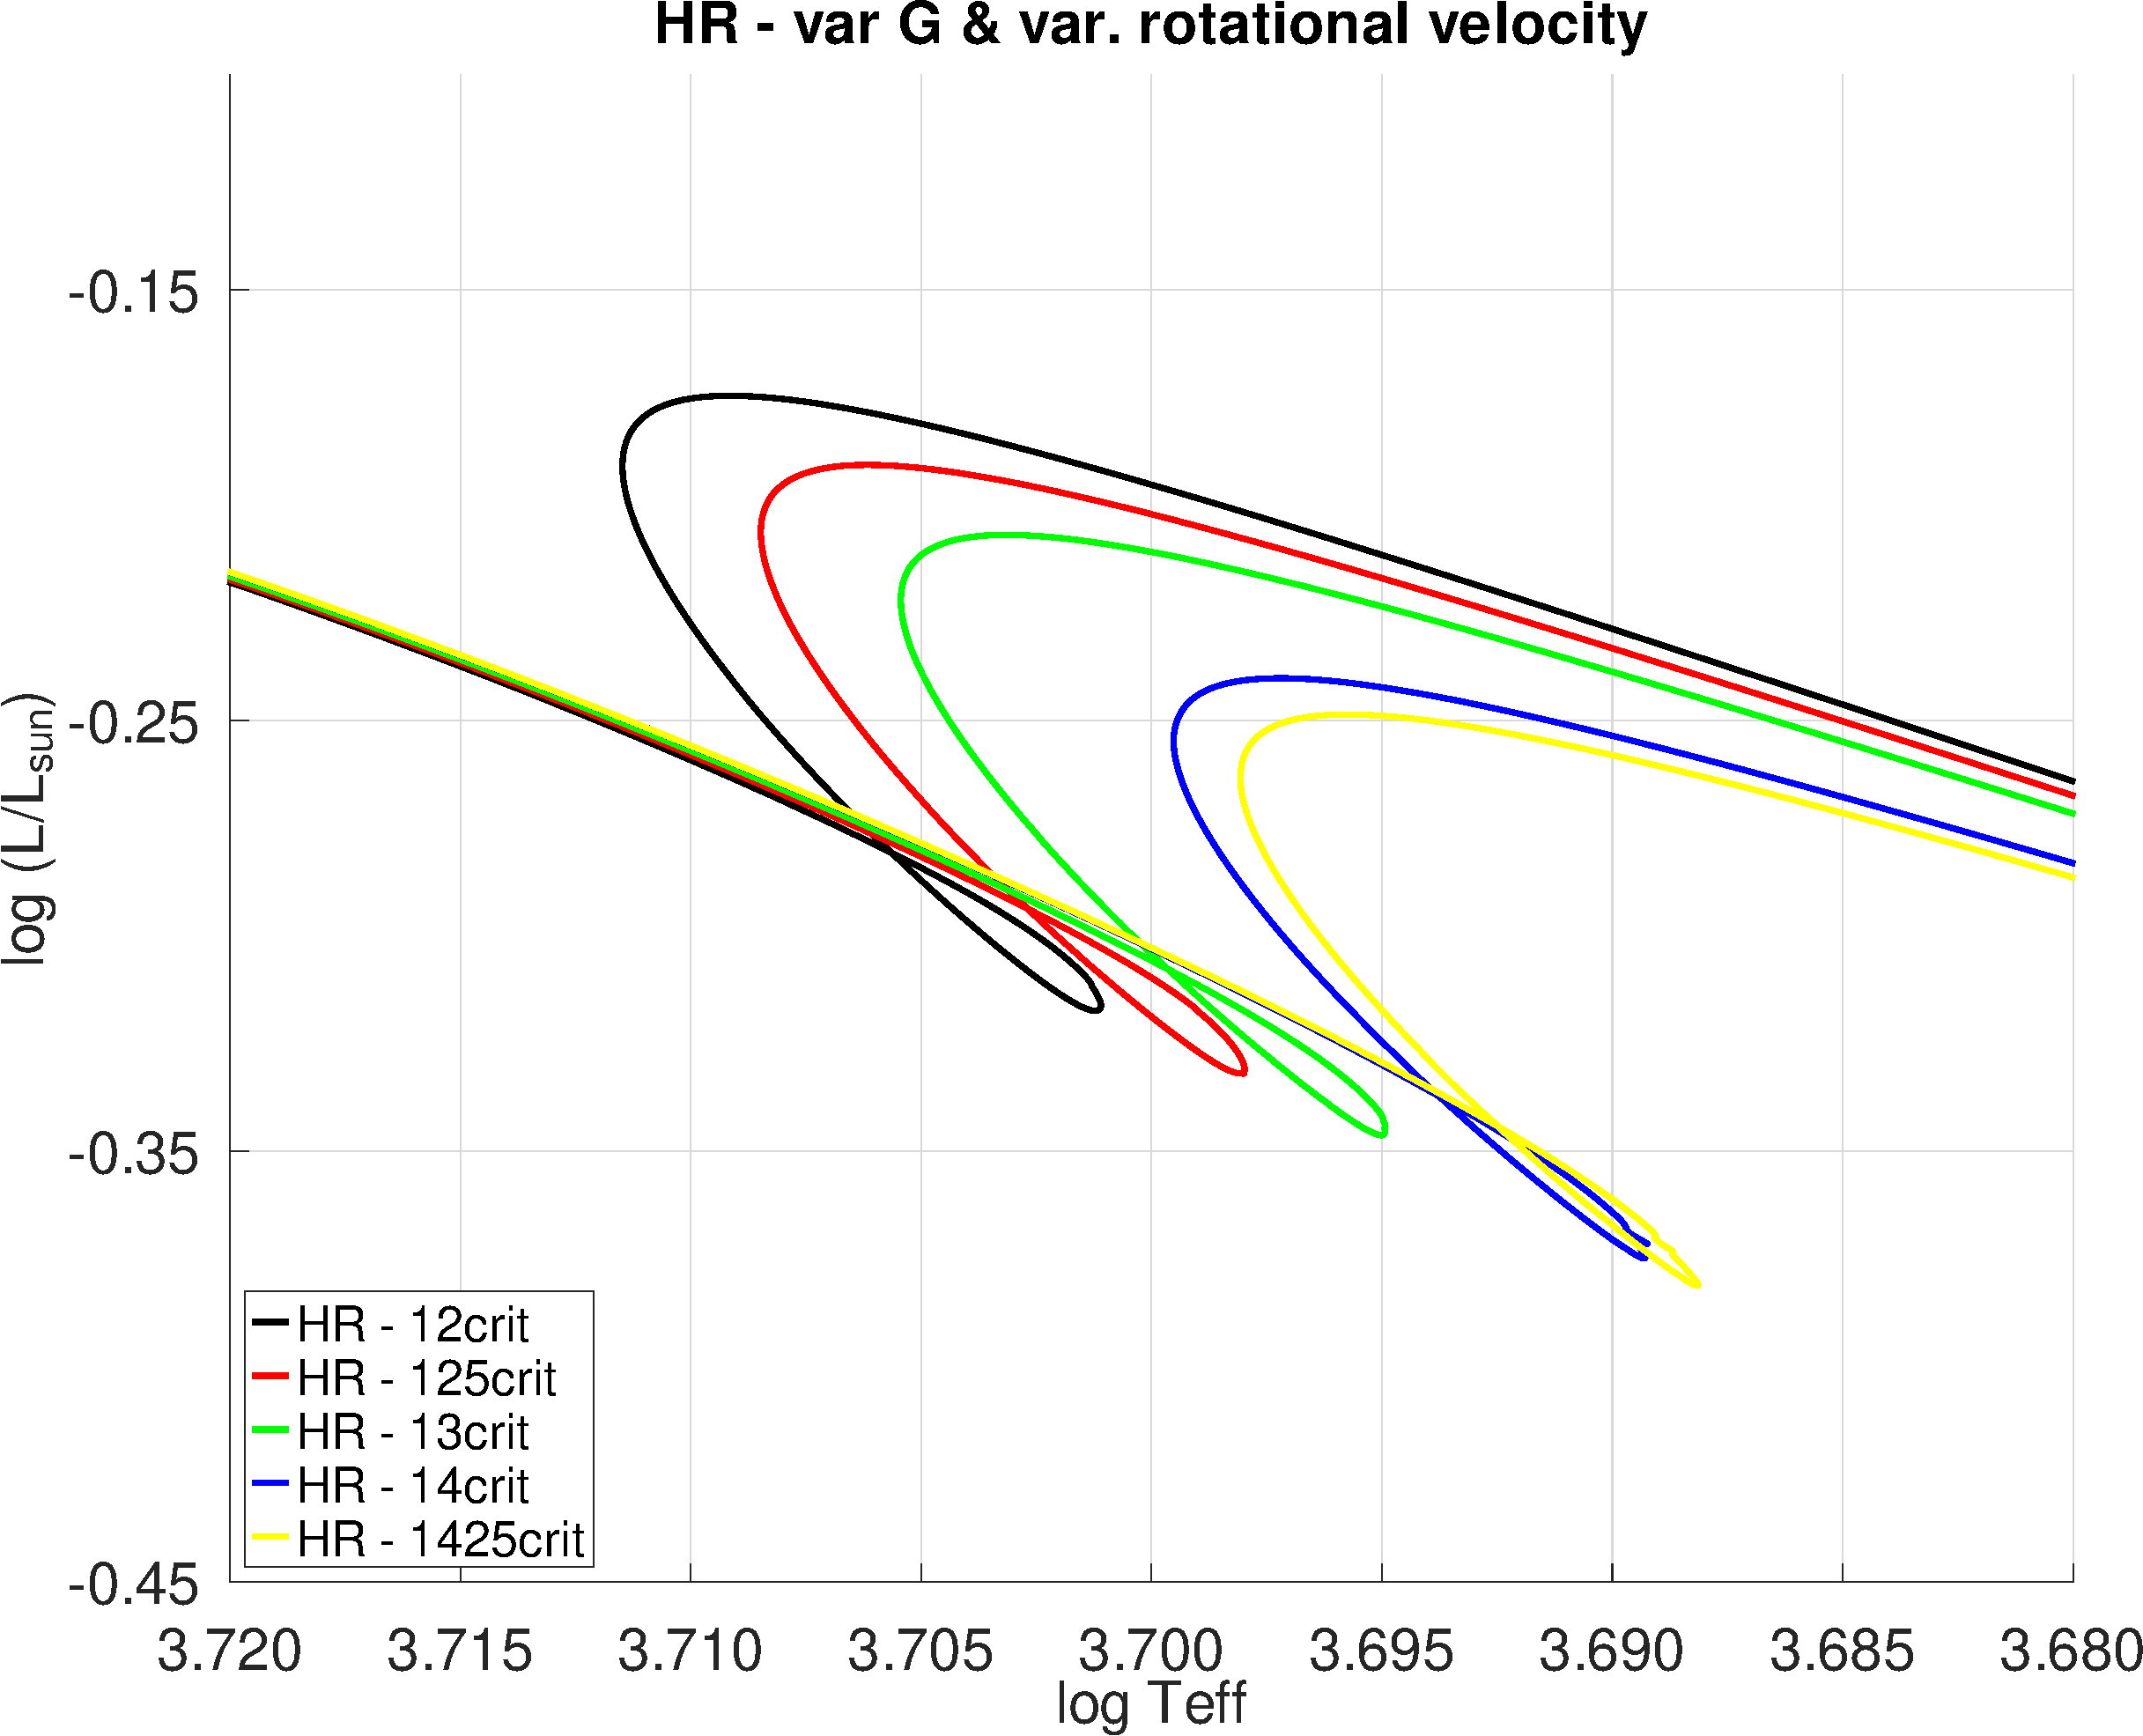
\includegraphics[width=0.7\textwidth]{img/paper2/hr_var_vel_var_g_z13.pdf}
	\caption{Un ejemplo de cuadrícula solar de 1$\msun$ de huellas evolutivas estelares que cubre un rango de velocidades angulares. Muestra en detalle los efectos combinados del oscurecimiento gravitatorio y el frenado magnético en las huellas evolutivas. Los modelos incluyen un campo magnético de intensidad variable, rotación inicial con $\omegaini$ entre 0.12 y 0.1425. La presencia de un campo magnético produce estrellas más calientes debido a la influencia del frenado magnético en la velocidad de rotación de la estrella.}
	\label{fig:hr_var_vel_var_g_z13}
\end{figure}

\begin{figure}
	\centering
	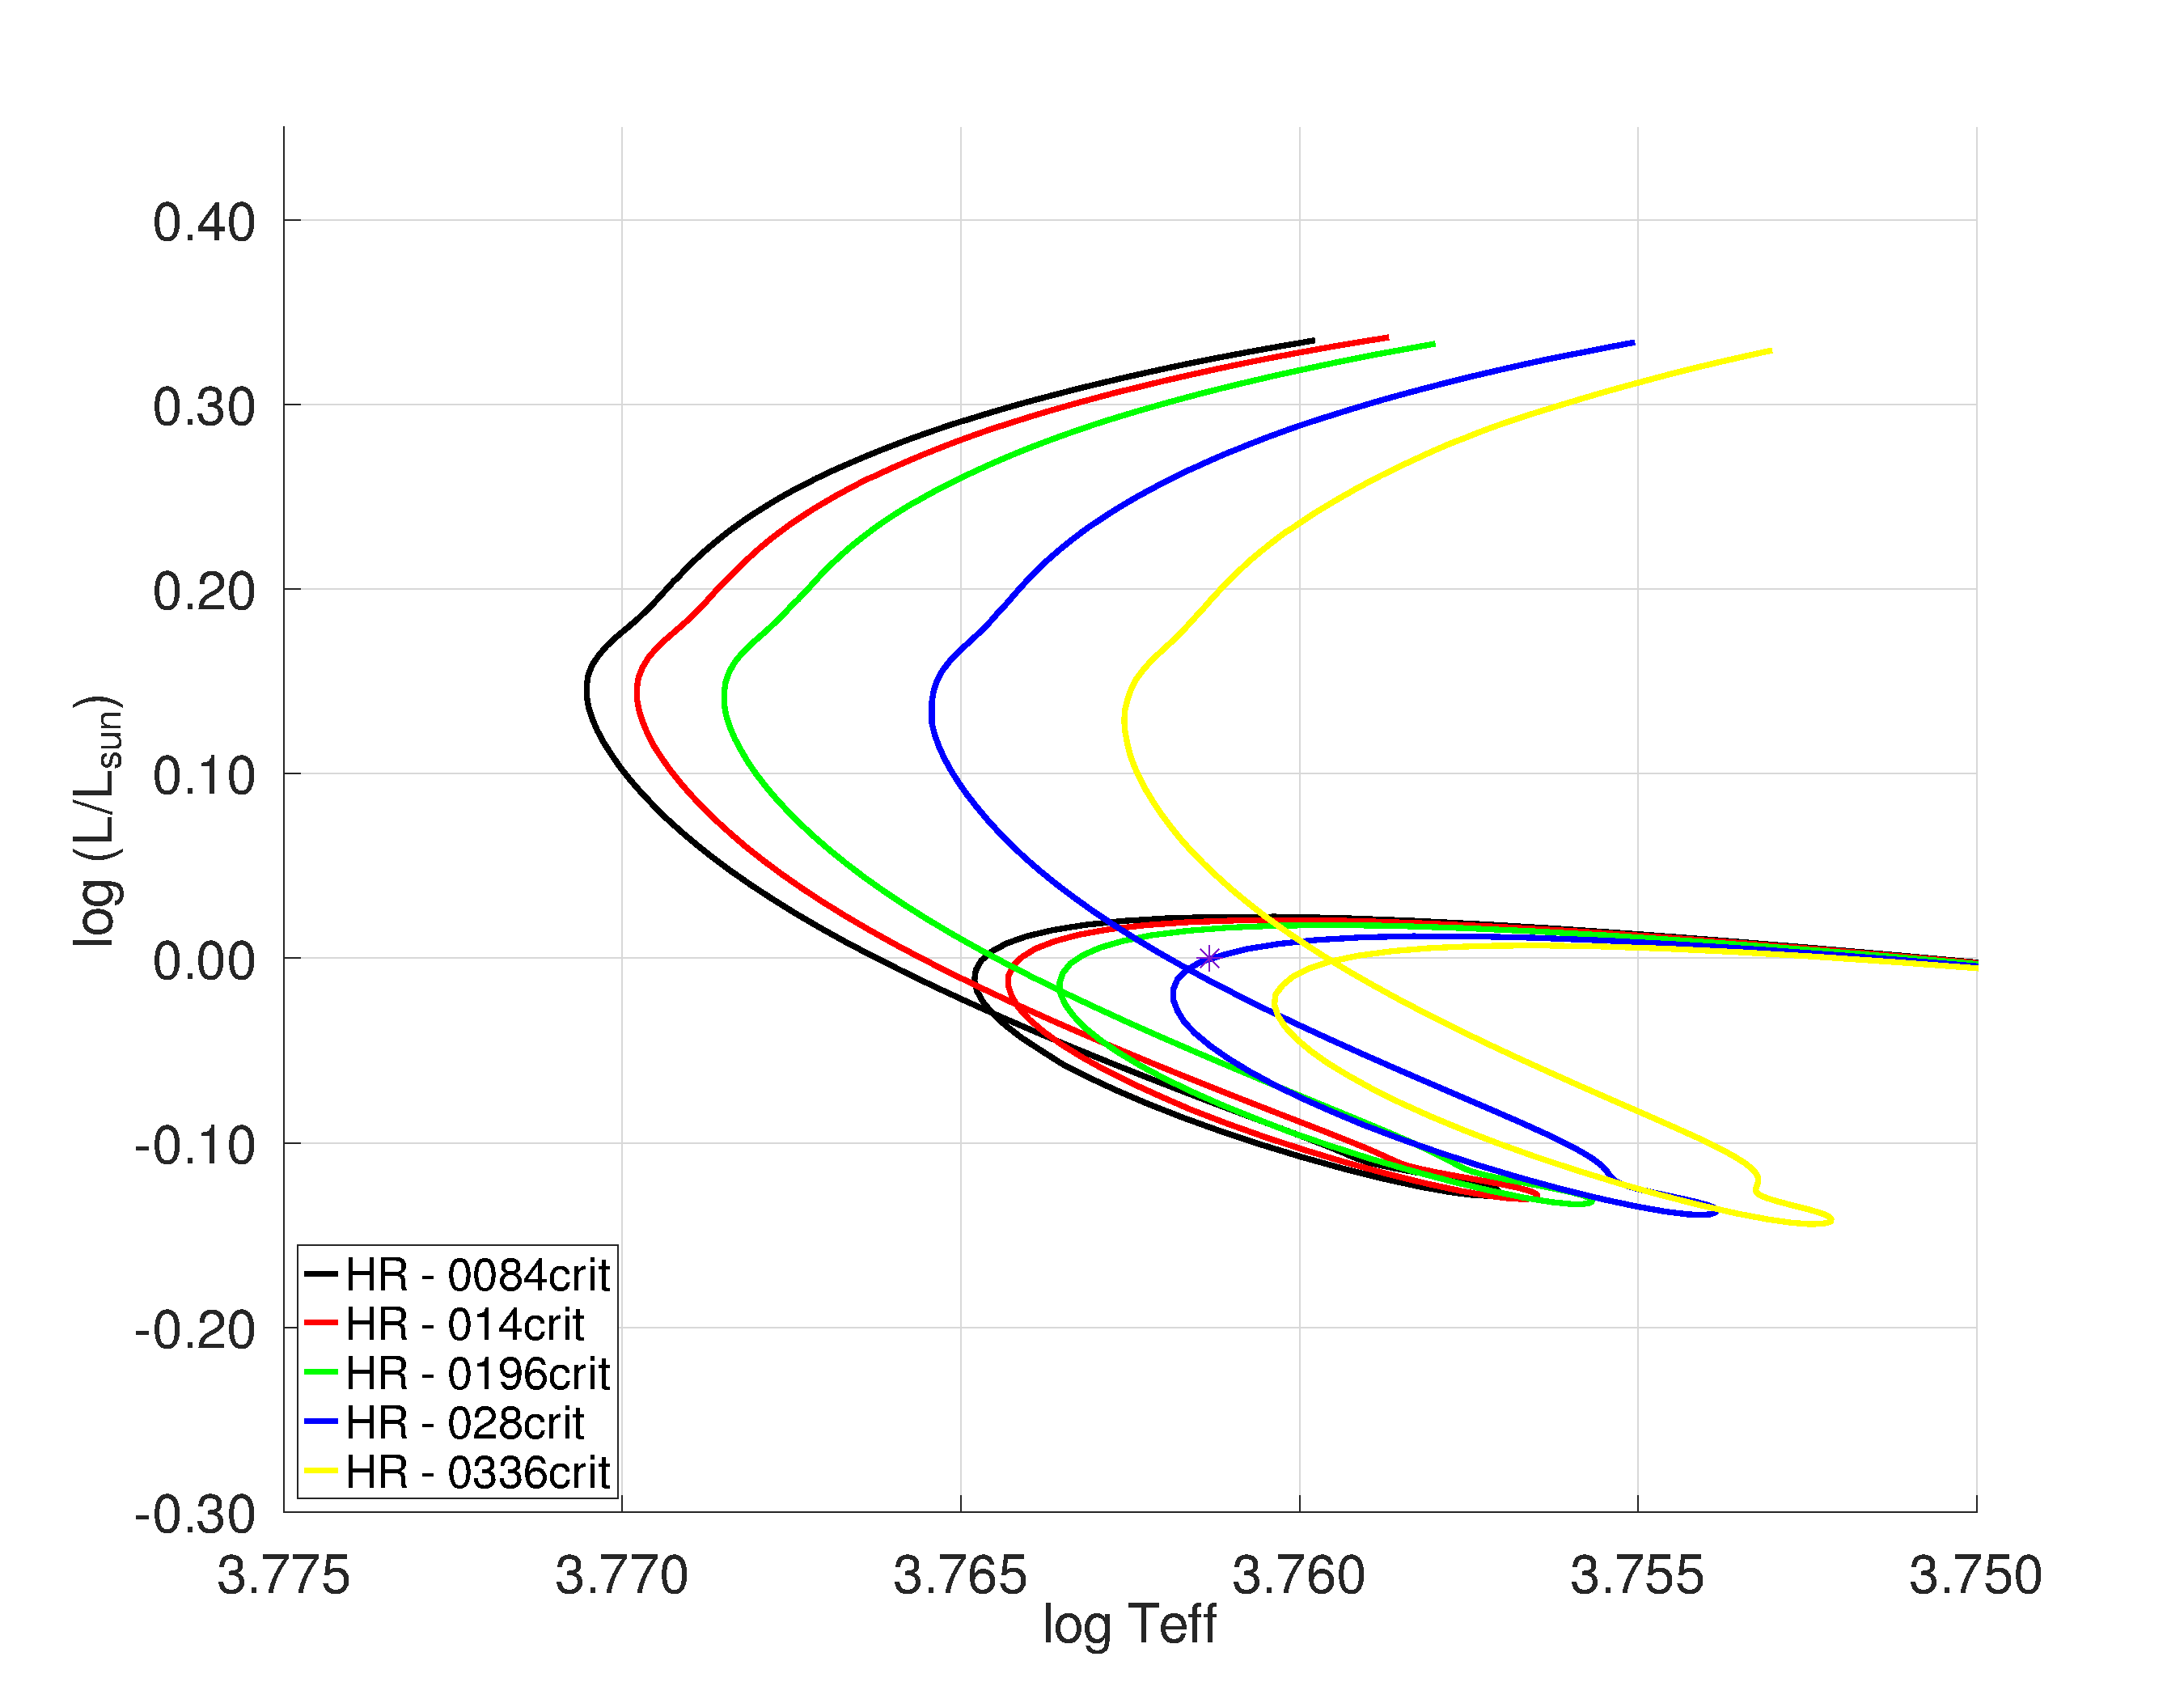
\includegraphics[width=0.7\textwidth]{img/paper2/hr_var_vel_0_0g_z10.pdf}
	\caption{Similar a la Figura \ref{fig:hr_var_vel_var_g_z13} pero mostrando ahora las trayectorias evolutivas estelares en ausencia (0G) de un campo magnético. La rotación se activa en los modelos en el PMS y esos modelos llegan antes a la ZAMS y a un $\teff$ menor que el que no rota (línea negra sólida). La luminosidad se expresa en términos de $\lsun$. $\lsun$ = 3.761. (Figura tomada de \cite{Caballero2020}.)}
	\label{fig:hr_var_vel_0g}
\end{figure}

La figura \ref{fig:teff_logg_var_vel_g3} muestra cómo se comportan $\teff$ y $\gsurf$ a lo largo de la evolución de los modelos. Para aquellos con una mayor velocidad de rotación, observamos que tanto su temperatura como su gravedad superficial son menores que en los modelos de rotación más lenta, en consonancia con el oscurecimiento de la gravedad. Cabe destacar que en la fase de aproximación ZAMS observamos para el modelo de rotación más rápida (amarillo) que su gravedad superficial es mayor que la del resto de modelos más lentos. Esto puede explicarse observando la Figura \ref{fig:lograd_var_vel_g3}, que muestra la evolución del radio estelar para los distintos modelos, en función del tiempo y $\omegaini$. Alrededor del intervalo de $2.5x10^{7}$ y $3.5x10^{7}$ Ga (delimitado por las líneas cian) y después de la ZAMS, desde alrededor de $5.4x10^{7}$ a $11.2x10^{7}$ Ga (delimitado por las líneas magenta) el radio estelar del modelo más rápido es menor que el del resto, produciendo un $\gsurf$ mayor, y esto a su vez significa una menor pérdida de masa (véase la Fig. \ref{fig:mdot_var_vel_g3}). Durante este período el modelo más rápido lo hace a un ritmo menor y expone una gravedad superficial mayor. Recordemos que el radio estelar tiene una influencia inversamente cuadrática en el valor de $\gsurf$. Esta "anomalía" desaparece en cuanto el radio estelar vuelve a ser mayor para el modelo más rápido.\par


\begin{figure}
	\centering
	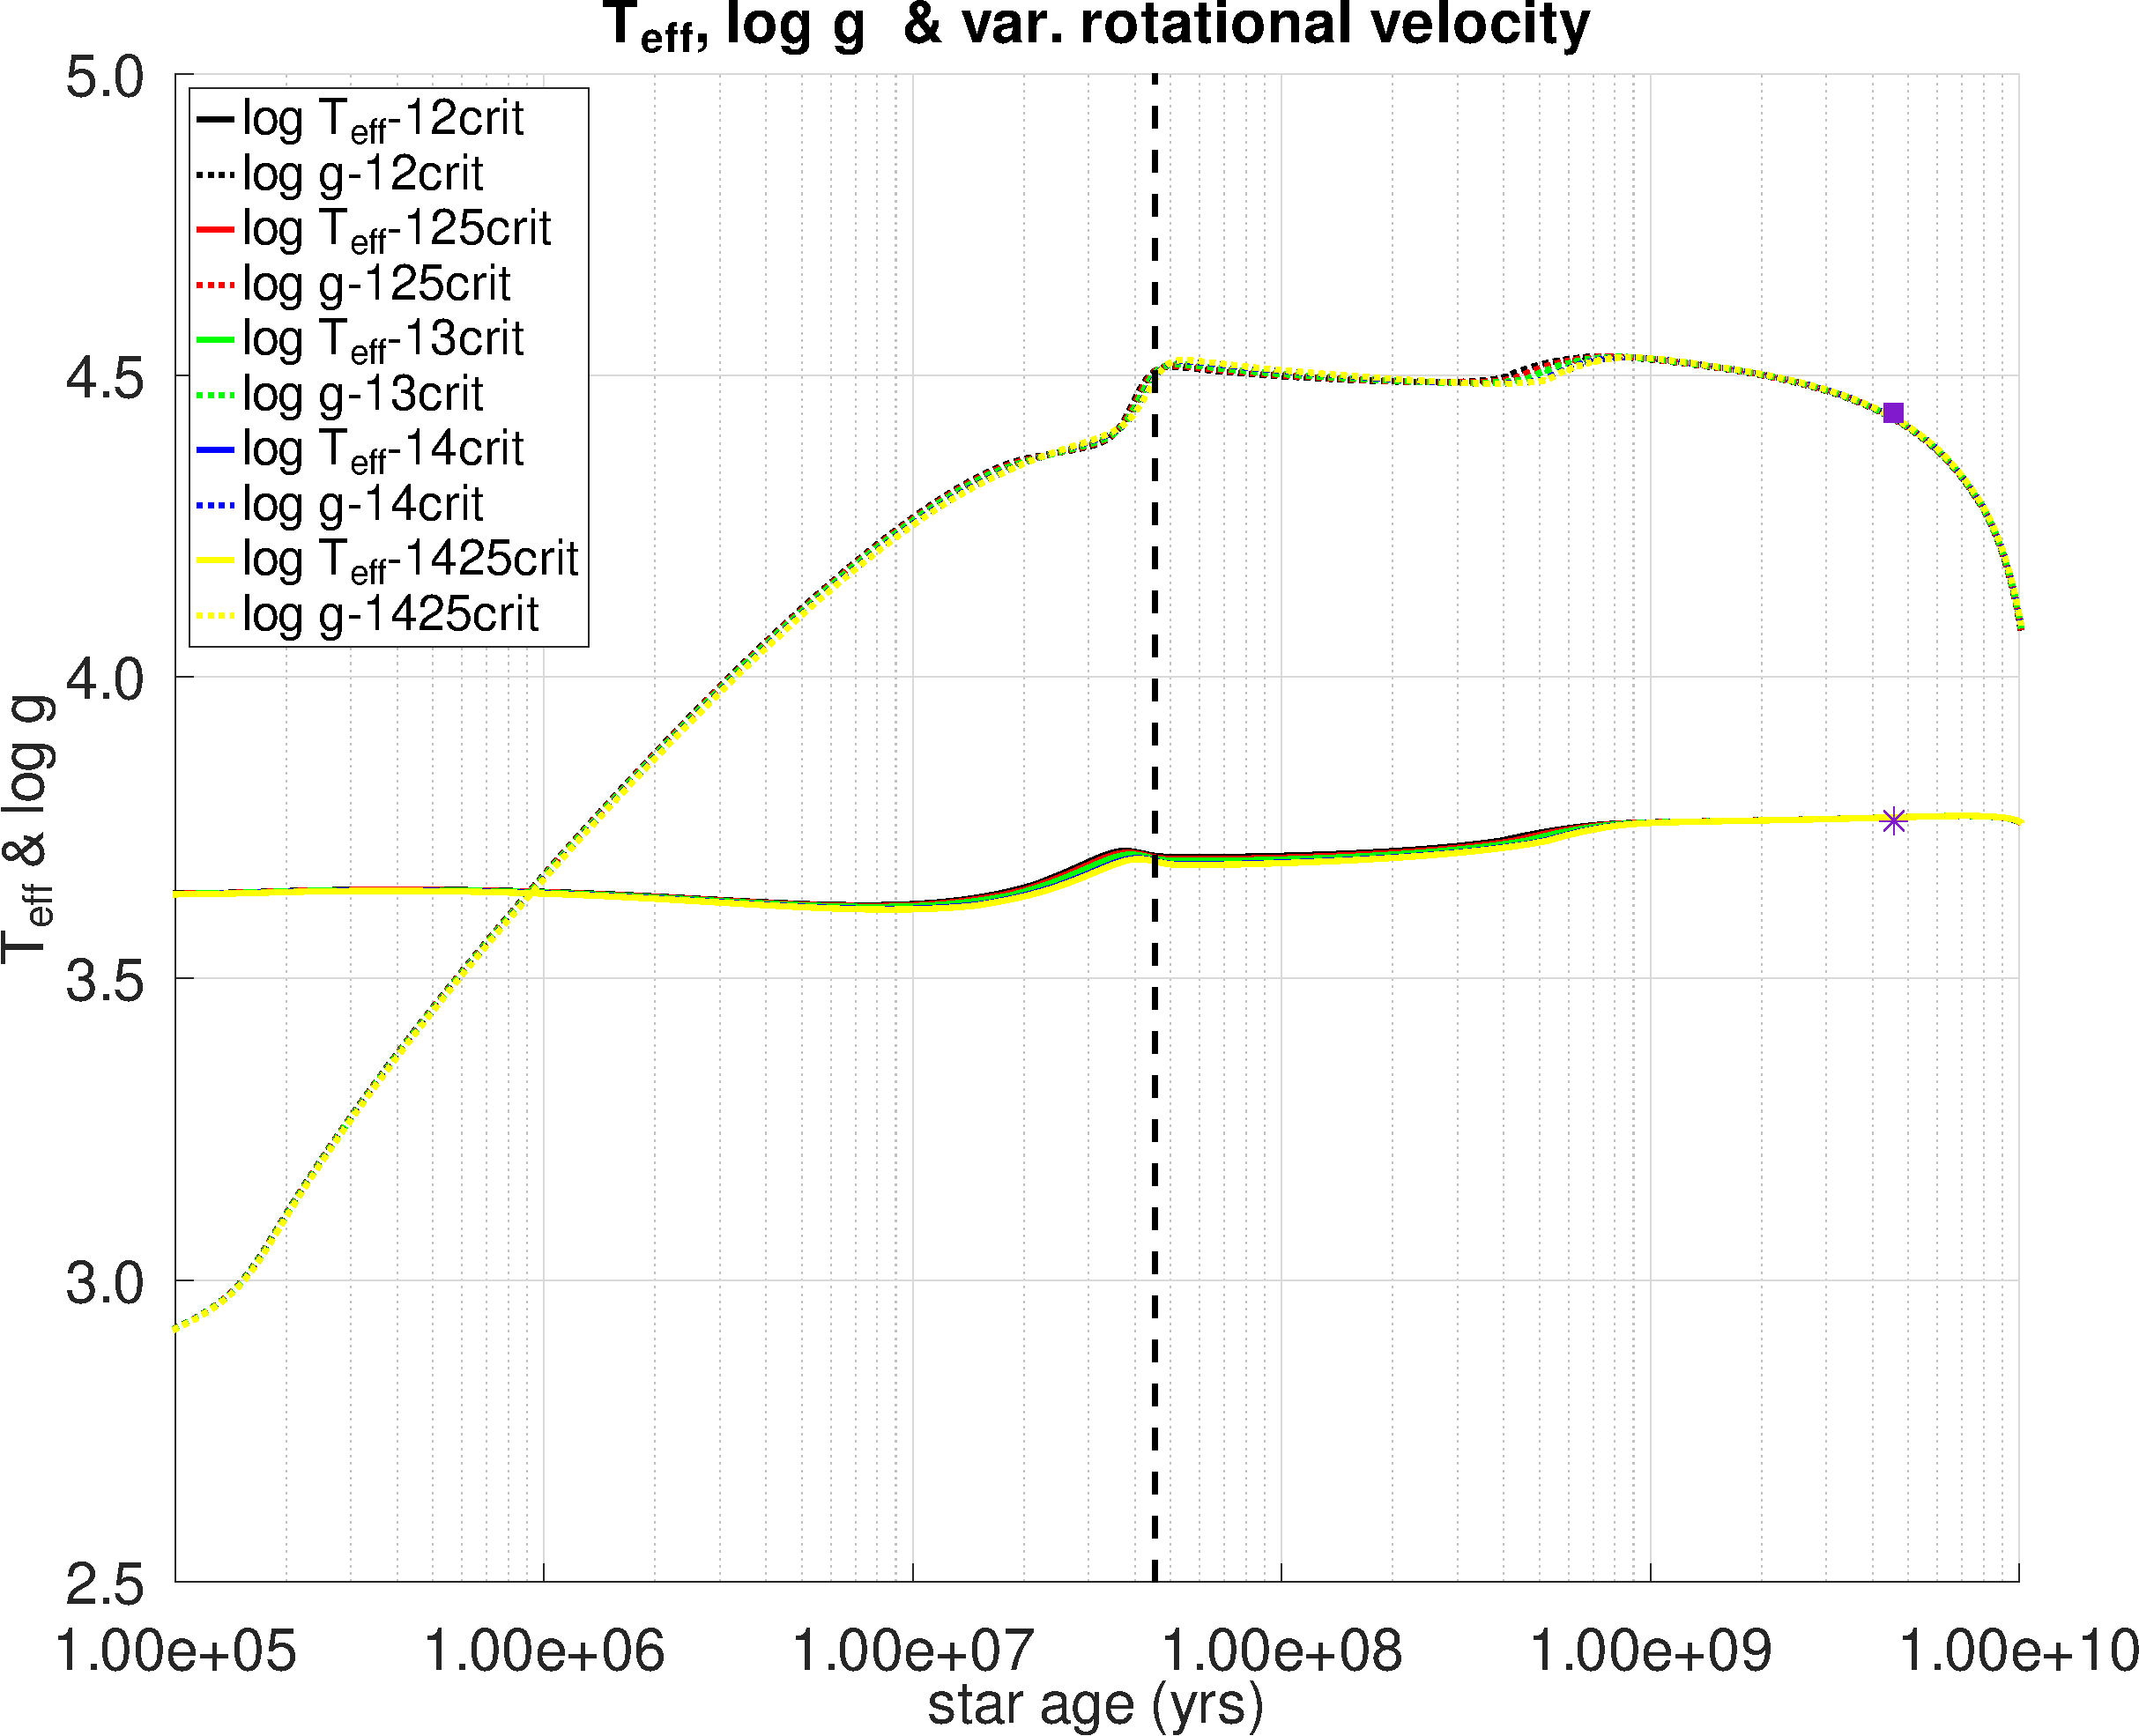
\includegraphics[width=0.7\textwidth]{img/paper2/teff_logg_var_vel_g3.pdf}
	\caption{La evolución de $\teff$ y $\gsurf$, en función del tiempo y $\omegaini$ para varios modelos de 1 $\msun$. Los modelos incluyen una rotación inicial con $\omegaini$ entre 0.12 y 0.1425. Los intervalos de edad [$2.5x10^{7},3.5x10^{7}$] Ga y [$5.4x10^{7},11.2x10^{7}$] Ga, delimitados por las líneas cian y magenta respectivamente, destacan periodos en los que el modelo más rápido con $\omegaini$=0,1425 expone una gravedad superficial superior a la del resto de los más lentos. La estrella morada es el $\teff$, y el cuadrado morado es la $\gsurf$ para el Sol actual \cite{Gill2012}. La línea vertical discontinua hace referencia a la ZAMS.}
	\label{fig:teff_logg_var_vel_g3}
\end{figure}

\begin{figure}
	\centering
	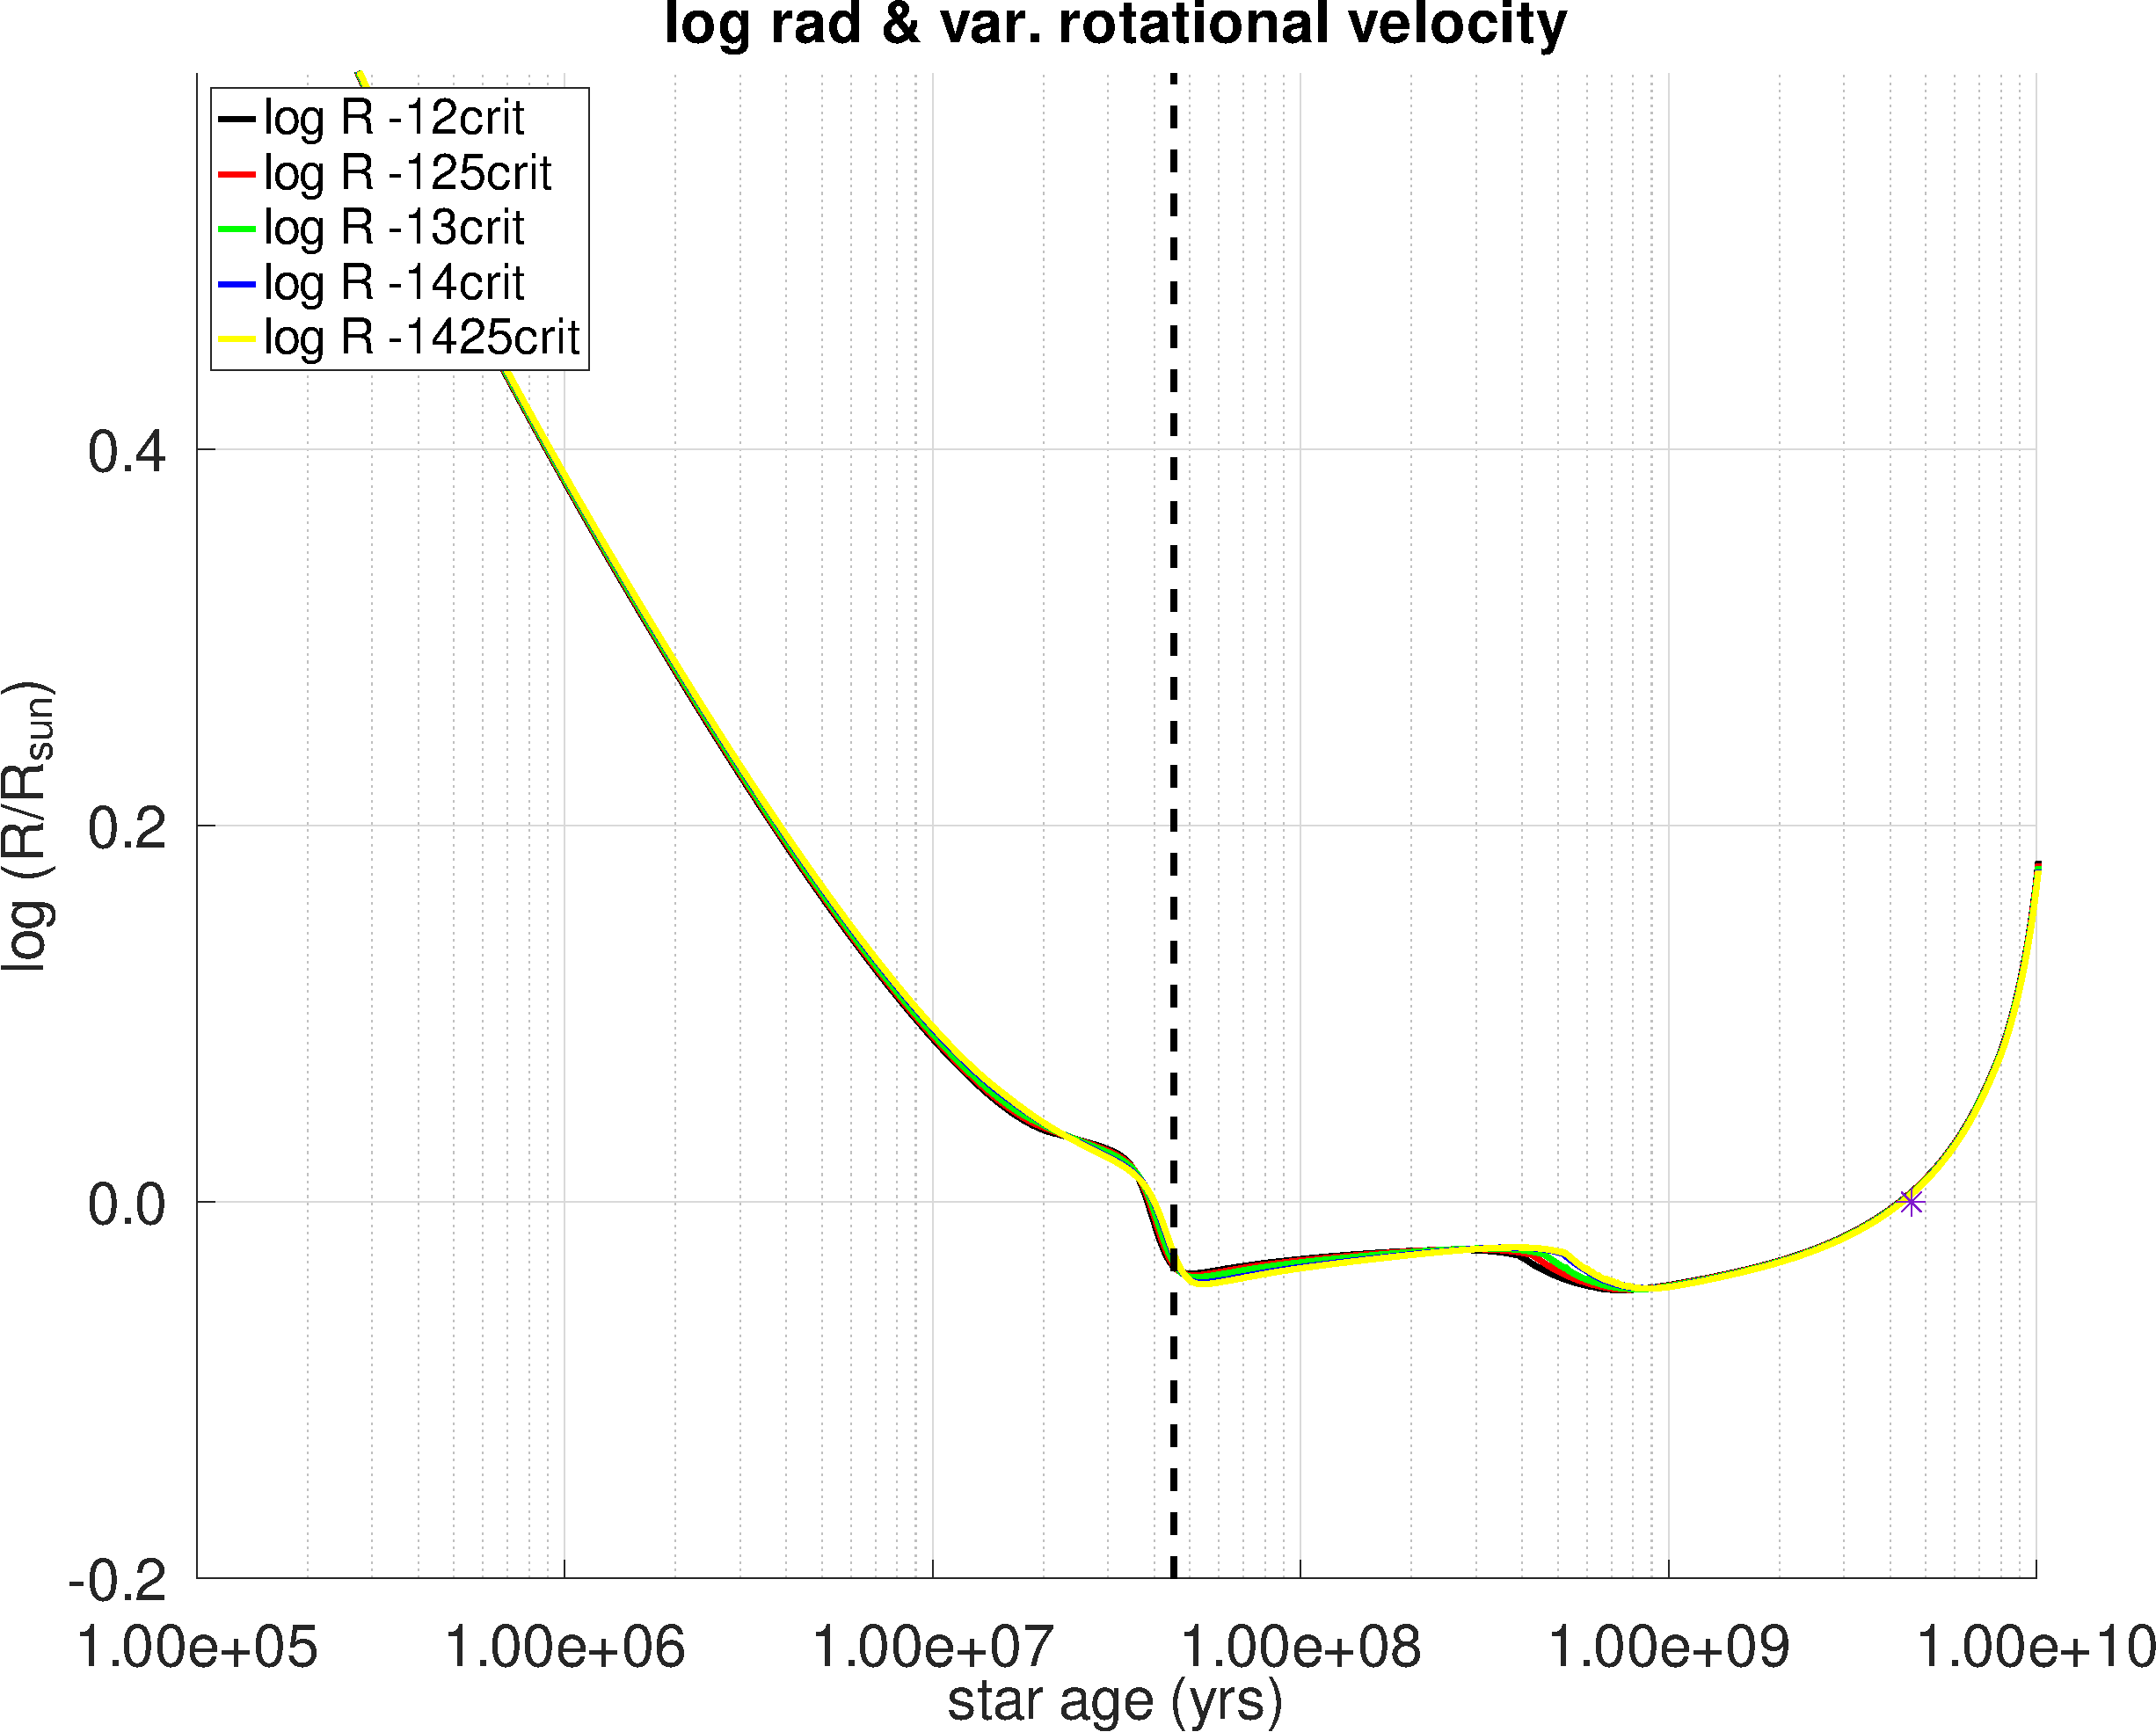
\includegraphics[width=0.7\textwidth]{img/paper2/lograd_var_vel_g3.pdf}
	\caption{La evolución del radio estelar, en función del tiempo y $\omegaini$ para varios modelos de 1 $\msun$ y sus. Los modelos incluyen rotación inicial con $\omegaini$ entre 0.12 y 0.1425. La estrella púrpura es el radio para el Sol actual \cite{Gill2012}. La línea vertical discontinua hace referencia a la ZAMS.}
	\label{fig:lograd_var_vel_g3}
\end{figure}


\section{Comparativa MB intensidad fija vs variable}
\section{Conclusiones}

\endinput
%--------------------------------------------------------------------
% FIN DEL CAPÍTULO. 
%--------------------------------------------------------------------



% -------------------------------------------------------------------
% APPENDIX: Opcional
% -------------------------------------------------------------------
\appendix % Reinicia la numeración de los capítulos y usa letras para numerarlos
\pdfbookmark[-1]{Apéndices}{appendix} % Alternativamente podemos agrupar los apéndices con un nuevo \part{Apéndices}

% !TeX root = ../libro.tex
% !TeX encoding = utf8

\chapter{Primer apéndice}\label{ap:apendice1}

Los apéndices son opcionales.

Archivo: \texttt{apendices/apendice01.tex}

\endinput
%------------------------------------------------------------------------------------
% FIN DEL APÉNDICE. 
%------------------------------------------------------------------------------------

% Añadir tantos apéndices como sea necesario 

% -------------------------------------------------------------------
% GLOSARIO: Opcional
% -------------------------------------------------------------------
\printglossary[type=\acronymtype, title=Acrónimos, toctitle=Acrónimos]
\printglossary[title=Glosario, toctitle=Glosario]

%% !TeX root = ../libro.tex
% !TeX encoding = utf8

\chapter*{Glosario}
\addcontentsline{toc}{chapter}{Glosario} % Añade el glosario a la tabla de contenidos

La inclusión de un glosario es opcional.

Archivo: \texttt{glosario.tex}

\begin{description} 
  \item[$\mathbb{R}$] Conjunto de números reales.

  \item[$\mathbb{C}$] Conjunto de números complejos.

  \item[$\mathbb{Z}$] Conjunto de números enteros.
\end{description}
\endinput
 

% -------------------------------------------------------------------
% BACKMATTER
% -------------------------------------------------------------------

\backmatter % Desactiva la numeración de los capítulos
\pdfbookmark[-1]{Referencias}{BM-Referencias}

% BIBLIOGRAFÍA
%-------------------------------------------------------------------

\bibliographystyle{alpha-es.bst} 
\begin{small} 
  \bibliography{library.bib}
\end{small}


\end{document}
